\documentclass[UTF8,openany,11pt,a4paper]{ctexbook}
\usepackage[margin=2.25cm,headheight=15pt]{geometry}
\usepackage{amsmath,amssymb,amsthm,bm,mathtools}
\usepackage{graphicx,booktabs,tabularx,longtable,multirow,array,calc}
\usepackage{float,subcaption,caption,xcolor}
\usepackage{xurl,hyperref,cleveref}
\usepackage{fancyhdr,enumitem,listings}
\usepackage{siunitx,etoolbox,tikz}
\usetikzlibrary{arrows.meta,positioning,shapes.geometric,fit,calc}
\IfFontExistsTF{Noto Serif CJK SC}{\setCJKmainfont{Noto Serif CJK SC}[AutoFakeSlant=0.15]}{\setCJKmainfont{FandolSong-Regular}}
\IfFontExistsTF{Noto Sans CJK SC}{\setCJKsansfont{Noto Sans CJK SC}}{\setCJKsansfont{FandolHei-Regular}}
\IfFontExistsTF{Noto Sans Mono CJK SC}{\setCJKmonofont{Noto Sans Mono CJK SC}}{\setCJKmonofont{FandolFang-Regular}}
\IfFontExistsTF{Linux Libertine O}{\setmainfont{Linux Libertine O}}{\setmainfont{TeX Gyre Termes}}
\IfFontExistsTF{DejaVu Sans}{\setsansfont{DejaVu Sans}}{\setsansfont{TeX Gyre Heros}}
\IfFontExistsTF{DejaVu Sans Mono}{\setmonofont{DejaVu Sans Mono}[Scale=0.83]}{\setmonofont{Latin Modern Mono}[Scale=0.83]}
\definecolor{navy}{RGB}{22,52,83}
\definecolor{teal}{RGB}{0,97,104}
\definecolor{lightgray}{RGB}{245,247,249}
\hypersetup{colorlinks=true,linkcolor=navy,urlcolor=teal,citecolor=teal,pdftitle={机器学习及其在天文与物理中的应用},pdfauthor={教材编写工作稿}}
\sisetup{detect-all,output-decimal-marker={.}}
\setlength{\emergencystretch}{2em}
\setlength{\parindent}{2em}
\setlength{\parskip}{2.5pt plus 1pt}
\linespread{1.20}
\setlist{itemsep=1pt,topsep=3pt}
\captionsetup{font=small,labelfont=bf}
\lstset{language=Python,basicstyle=\ttfamily\small,keywordstyle=\color{navy}\bfseries,commentstyle=\color{teal},stringstyle=\color{red!55!black},breaklines=true,frame=single,rulecolor=\color{black!20},backgroundcolor=\color{lightgray},numbers=left,numberstyle=\tiny\color{black!45},showstringspaces=false,tabsize=4,columns=fullflexible,keepspaces=true,aboveskip=8pt,belowskip=8pt}
\newcounter{worked}[chapter]
\newcommand{\worked}[1]{\refstepcounter{worked}\subsubsection*{例\thechapter.\arabic{worked}\quad #1}}
\BeforeBeginEnvironment{lstlisting}{\par\noindent\begin{minipage}{\linewidth}}
\AfterEndEnvironment{lstlisting}{\end{minipage}\par}
\newcommand{\keypoint}[1]{\par\noindent\textbf{核心理解：}#1\par}
\newcommand{\scientificnote}[1]{\par\noindent\textbf{科学数据注意：}#1\par}
\newcommand{\chaptergoal}[1]{\section*{本章学习目标}\addcontentsline{toc}{section}{本章学习目标}#1}
\newcommand{\chapterpractice}[1]{\section*{本章实践与交付}\addcontentsline{toc}{section}{本章实践与交付}#1}
\newcommand{\chapterexercise}{\section*{练习与讨论}\addcontentsline{toc}{section}{练习与讨论}}
\newcommand{\fig}[3][0.83]{\begin{figure}[htbp]\centering\includegraphics[width=#1\linewidth]{figures/#2}\caption{#3}\end{figure}}
\providecommand{\real}[1]{#1}
\setcounter{secnumdepth}{2}
\setcounter{tocdepth}{1}
\hypersetup{bookmarksdepth=2}
\pagestyle{fancy}
\fancyhf{}\fancyhead[LE,RO]{\small\nouppercase{\leftmark}}\fancyfoot[C]{\thepage}
\renewcommand{\headrulewidth}{0.4pt}
\raggedbottom
\begin{document}
\frontmatter
\begin{titlepage}
\centering\vspace*{4cm}
{\sffamily\bfseries\Huge 机器学习及其在天文与物理中的应用\par}
\vspace{1.1cm}{\Large 面向非计算机专业本科生的概念、经典算法与实践\par}
\vspace{3cm}{\large 概念与案例教学修订版\par}
\vspace{1cm}{\large 2026年11月\par}
\vfill{\small 广州大学天体物理中心 王锋\par}
\end{titlepage}
\chapter*{前言}

物理学和天文学通过观测、实验与理论研究认识自然。在这一过程中，数据分析承担着连接测量与科学认识的重要任务：从观测量中识别天体类型，根据实验条件预测物理量，在多维数据中寻找共同特征，以及发现值得进一步研究的特殊对象。这些问题具有不同的专业背景，却往往涉及相似的分析过程：明确研究目标，组织测量数据，建立模型，检验结果，并结合专业知识作出解释。机器学习为这一过程提供了一组重要的方法。

本书面向物理学、天文学及相关理科专业本科生，介绍机器学习的基本概念、经典算法及其应用。全书以理解模型和解决问题为主线，着重回答三个问题：模型依据什么作出判断，学习算法怎样从数据中建立模型，以及怎样评价模型在实际任务中的表现。通过学习，读者应当能够把一个专业问题转化为明确的建模任务，选择适当的方法，完成数据处理与模型比较，并解释结果的意义。

理解算法需要直观认识，也需要必要的数学表达。本书从具体问题和小规模数据出发，通过定义、图示、逐步计算和对照实验建立概念之间的联系。例如，从预测误差引出损失函数，从参数更新理解梯度下降，从候选划分的比较理解决策树，再通过模型组合认识随机森林和梯度提升。对于能够解释模型行为的推导，正文给出主要步骤；较长的证明和进一步的理论讨论安排在选学内容中。数学表达与程序实验相互配合，帮助读者理解方法的依据及其实际效果。

全书共17章，分为四个部分。第一部分介绍机器学习任务、数据表示与准备、损失函数与优化，以及模型评价和泛化，为后续学习建立共同基础。第二部分介绍线性回归、逻辑回归、近邻方法、决策树、随机森林、梯度提升、支持向量机和多层感知机，涵盖主要的经典监督学习方法，并由此进入神经网络的学习。第三部分讨论主成分分析、聚类和异常检测，研究如何在缺少目标标签时分析数据的表示与结构。第四部分围绕模型解释、误差分析和科学结论，组织天文与物理综合项目，将前面的知识用于完整的分析任务。

案例按照由熟悉数据到专业问题的顺序展开。入门阶段使用鸢尾花测量、葡萄酒化学分析和区域住房统计等数据，分别建立分类与回归的基本认识。同一组数据会在不同章节中反复使用，使读者能够在熟悉的问题上比较模型的机制和表现。随后引入手写数字图像、天体目录和物理实验数据，逐步增加特征选择、测量误差、样本划分和专业解释等方面的要求。每个案例都从研究对象、数据含义和分析目标出发，使算法学习始终与具体问题相联系。

实验采用Python编程语言，以scikit-learn作为主要的机器学习工具，并使用Pandas整理表格、NumPy进行数值计算、Matplotlib绘制图形。各章实验与原理讲解相互对应：读者先根据模型机制判断可能出现的现象，再运行程序，通过改变特征、参数或训练条件检验自己的理解。实验分析既关注评价指标，也关注错误样本、结果波动和模型失效的情形。配套习题包括概念辨析、数值计算、结果解释和专业迁移，帮助读者逐步从复现示例走向独立分析。

本书适合首次系统学习机器学习的理科本科生。读者应具备基础的高等数学、线性代数、概率统计和Python编程知识，学习中需要用到的数学与程序概念会结合具体内容进行回顾。全书可用于64学时课程，教师可以根据学生基础选择课堂重点，将部分推导、提高练习和综合项目安排在课外。独立阅读时，建议先理解例题中的计算过程，再完成程序实验，并用自己的语言说明每一步的目的与结果。

机器学习的应用能力，体现在从问题到结论的整个过程之中。一个合适的模型，需要与明确的目标、可靠的数据和合理的评价方法共同发挥作用；一个有价值的结果，则需要结合观测条件、实验背景和专业知识加以理解。希望读者通过本书的学习，既掌握经典机器学习方法，也逐步形成提出问题、检验证据和解释结果的习惯，为进一步的课程学习与科学研究打下基础。

\tableofcontents
\mainmatter
\part{机器学习基础}
\chapter{机器学习的基本概念与任务}
\label{chap:concepts}
\chaptergoal{学完本章，应能从一张具体数据表中指出样本、输入特征和目标；用自己的话解释模型、训练与预测；区分监督学习与无监督学习，以及分类、回归、聚类和降维任务。阅读本章不需要预先认识任何机器学习算法。}

假设实验室已经记录了不同输入信号下传感器的输出。现在输入一个新的信号，我们希望在测量之前估计传感器将给出什么数值。又假设已经测量了一批花的尺寸，并由专家确定了它们的物种；面对一朵尚未辨认的花，我们希望根据尺寸判断其物种。这两个问题的对象不同，但都希望借助已有记录，对新对象作出判断。

本章从这些具体问题开始。我们先读懂数据，再为其中的对象和操作命名。代码只是把思路交给计算机的表达方式；在知道数据是什么、要解决什么问题之前，不需要急于训练一个模型。

\section{从天文与物理问题到机器学习任务}
\subsection{什么是机器学习}
\textbf{机器学习（machine learning）是利用已有数据，按照明确的学习目标建立或调整计算规则，以完成预测、识别或数据结构分析的一类方法。}这里的“学习”不是计算机理解了对象的全部含义，而是规则的某些部分由数据确定，而非全部由人逐条写出。

例如，人可以先规定“输入信号每增加一个单位，预测输出增加两个单位”。这是一条人工给定的规则。另一种做法是收集输入与输出的配对记录，让计算程序寻找一条较贴近这些记录的直线。后一种方法中，直线的斜率和截距由数据决定，是本书讨论的数据学习过程。选择什么形式的规则、依据什么标准认为它合适，仍需要人作出规定。

一组为某项分析整理在一起的数据记录称为\textbf{数据集（dataset）}。数据集可以是表格、图像集合或一系列测量曲线。本书首先使用表格：一行记录一个分析对象，一列记录对象的一项信息。表格的含义由任务决定，不是所有列都要送入模型。

\subsection{先说清要完成什么工作}
在天文学中，可以根据天体在不同波段的亮度判断它是恒星还是星系。恒星是类似太阳的发光天体，星系则由大量恒星、气体等构成；这里希望预测的是一个类别。在物理实验中，可以根据气流速度、声波频率等条件预测测得的声压级；这里希望预测的是一个数值。还可以只观察一批测量记录，寻找彼此相似的群体，而不预先告诉程序每条记录属于哪一类。

这些不同的要求称为\textbf{任务}。预测类别、预测数值和寻找群体不是同一个任务，所需数据和评价方式也不同。暂时不必记住所有算法名称；首先把问题写成一句能检查的陈述，例如：“输入一朵花的四项尺寸，输出三个已知物种中的一个。”

物理理论和机器学习可以共同服务于研究。理论模型通常依据物理假设写出关系；数据模型依据已有记录确定预测规则。两者都需要检查适用范围。即使一个规则能够预测观测结果，也还需要另外的证据才能把它解释为物理机制。本章先学会建立预测问题，科学解释在第16章展开。

\subsection{把科学问题改写成可以检验的任务}
“研究恒星”是研究方向，还不是一个机器学习任务；“从一段光变曲线判断是否具有某类周期变化”才逐渐接近可以实施的问题。要继续说明曲线在什么时段获得、包含多少个测量点、参考类别怎样确定，以及以后遇到的新对象与现有对象有何关系。\textbf{任务的精确程度，决定了后面每一个技术选择是否有意义。}

以温度传感器为例，我们有两种不同需求。需求甲是根据传感器电压估计参考温度，部署时能测到电压，但不能总是使用昂贵的参考仪器。需求乙是根据已知温度、输入电压和仪器编号预测输出，检查设备是否偏离正常工作状态。两者都涉及相似的测量表，但预测目标不同，能够使用的输入也不同。不能因为表格相同，就沿用同一个任务描述。

\worked{一个可执行的任务说明}
假设实验室已在20件传感器上测量电压和参考温度，每件重复测量10次。现要给\emph{新的传感器}标定。样本表虽然有200行，独立设备只有20件；输入为部署时可得到的电压和环境温度，输出为参考仪器测得的温度。评价应让某些整件设备不参与建模，再检查对这些设备的预测。这是一个人为设定的任务，不是本书的真实仪器实验。

若目的改成给\emph{同一件已经见过的传感器}预测下一次测量，就可能使用该设备过去的记录。前者检查跨设备迁移，后者检查同设备上的重复应用。没有任何一种划分天然适用于两种目标。读者此时无需掌握具体拆分函数，但应能发现“样本到底是什么”和“将来会预测谁”是方法的一部分。

\subsection{预测关系不等于物理关系，二者仍可以协作}
一个模型可以先用物理分析构造有意义的输入，再用数据估计未知系数。例如运动学提示位移可能与时间和时间平方有关，回归程序负责估计相应系数。反过来，数据残差的系统变化也可以提示某个物理假设不充分。机器学习并不要求放弃专业知识，也不保证从未经整理的原始表中自动找到研究对象的本质。

本书区分三个层次。\textbf{预测层次}问新样本结果是否准确；\textbf{描述层次}问现有数据中哪些变量一起变化；\textbf{解释层次}问改变某个物理条件是否会导致结果改变，以及机制是什么。三者可能相互支持，但需要的证据不相同。例如仪器编号帮助识别设备，未必意味着编号本身决定测量值。后续章节中的模型分数首先属于预测层次。

\section{样本、特征、标签与目标变量}
\label{sec:iris-intro}
\subsection{先认识一组花的测量记录}
我们从\textbf{鸢尾花测量数据集（Iris dataset，后文简称鸢尾花数据）}开始。Iris 是这一数据集的英文名称，不是算法。数据中有150条花的测量记录，来自三个物种，每个物种50条；每条记录有四项尺寸测量，单位均为厘米。三个物种以 \textit{Iris setosa}、\textit{Iris versicolor} 和 \textit{Iris virginica} 记录。无需记忆拉丁名称，只需把它们看作三个不同类别。数据规模、字段与类别对应关系见官方数据说明\textsuperscript{[2,26]}。

四项尺寸是萼片长度、萼片宽度、花瓣长度和花瓣宽度。萼片与花瓣是花的两类结构；本例只需要理解它们被分别测量，不要求植物学知识。表\ref{tab:iris-records}摘取了三条实际记录。这里的“记录行号”仅用于找到这条记录，不是花的一项尺寸。

\begin{table}[htbp]\centering\small
\caption{鸢尾花数据中的三条记录。四项尺寸的单位均为厘米；编号为随书数据的零起始位置。}\label{tab:iris-records}
\begin{tabular}{rrrrrl}\toprule
记录行号&萼片长&萼片宽&花瓣长&花瓣宽&已知物种\\\midrule
0&5.1&3.5&1.4&0.2&setosa\\
50&7.0&3.2&4.7&1.4&versicolor\\
100&6.3&3.3&6.0&2.5&virginica\\\bottomrule
\end{tabular}
\end{table}

读第一行时，可以把它说成一句话：“这朵花的萼片长5.1厘米、宽3.5厘米，花瓣长1.4厘米、宽0.2厘米，已知物种为setosa。”表格中的数字和物种不是彼此独立的清单：它们属于同一朵花，必须保持对应。

\subsection{给数据表中的角色命名}
\textbf{样本（sample）}是本次分析中的一条对象记录。在本例中，一朵花的测量记录是一个样本，150行就是150个样本。\textbf{特征（feature）}是用于作出预测的输入信息；这里四项尺寸是四个特征。\textbf{目标变量（target）}是希望模型预测的量；这里希望预测物种，所以物种是目标。对于这种类别目标，本书也称其为\textbf{类别标签（class label）}。

“特征”和“目标”不是一个字段永远不变的属性，而是它在当前任务中的角色。如果问题改为根据其他尺寸预测花瓣长度，花瓣长度就成为目标，不再同时作为该任务的输入。每次建模都应先确定任务，再分开输入与目标。

用 $\mathbf x_i$ 表示第 $i$ 条记录的四个输入，第一行可写为
\[
\mathbf x_1=(5.1,3.5,1.4,0.2),\qquad y_1=\text{setosa}.
\]
这里下标1表示书写中的第一个样本，与表中零起始的程序行号0对应。把所有样本的输入逐行排列，得到\textbf{特征矩阵} $X$；把对应目标依次排列，得到目标序列 $y$。若有 $n$ 个样本、$p$ 个特征，$X$ 有 $n$ 行、$p$ 列，记作 $X\in\mathbb R^{n\times p}$。鸢尾花数据的输入形状就是 $(150,4)$，而不是 $(150,5)$；类别列不包含在输入矩阵中。

\subsection{数字编码不改变字段的含义}
程序可以把三个物种编码为0、1、2。它们只表示类别身份，不表示第三类比第一类“多两单位”，也不意味着类别1位于类别0与类别2之间。预测类别时，应核对数字与名称的对应关系，不能仅根据数字形式就把目标当作连续测量量。

一张专业表还可能有编号、测量时间和质量说明。编号用来识别对象，质量说明用来判断测量是否可靠，它们不一定作为预测输入。一个天体有三次观测时，表中可能出现三行，但只有一个科学对象。第一次读表就应知道“一行代表什么”，更复杂的分组问题留到第4章。

\subsection{一行数据与一个对象：重复测量为什么需要单独登记}
数据中的一行可以代表一件对象，也可以代表对象的一次测量。在天体目录中，\texttt{object\_id}可以识别天体，\texttt{observation\_id}识别一次观测；两者不能互相代替。一个对象被观测多次时，这些行可能共享几乎相同的真实物理性质。把所有行数直接当作独立对象数，会夸大数据提供的新信息。

第一次建立数据表时，可以让每行同时带有“行标识”和“对象标识”。前者用于追踪程序中的预测，后者用于识别相关测量。它们都不必自动进入模型。程序需要这些字段来保证可追踪性，模型则只接收任务允许的输入。\textbf{保存一列与把一列作为特征，是两个不同决定。}

\worked{把表格写成输入与目标}
用一个人工三行例子练习符号：三次测量的输入电压为1、2、3 V，环境温度为20、20、25摄氏度，参考输出为2.1、4.0、6.2 V。若预测参考输出，则
\[
X=\begin{pmatrix}1&20\\2&20\\3&25\end{pmatrix},\qquad
\mathbf y=\begin{pmatrix}2.1\\4.0\\6.2\end{pmatrix}.
\]
矩阵是三行两列，所以$n=3,p=2$。第2行的输入为$(2,20)$，不能与第3行目标6.2拼成一对。数据排序、删除缺失行或合并表格时，必须保持这种配对。机器学习程序通常无法从数值本身判断配对是否已经错位。

此时还没有学习模型。矩阵只是一种组织输入的方式；同一个$X$可以交给不同模型。把矩阵写出来有助于检查数据形状，但不会替代对每列的单位和含义的说明。

\section{模型、训练、预测与泛化}
\subsection{模型是一条可以计算的规则}
\textbf{模型（model）}是从输入产生输出的可计算规则。比如，给定一个长度 $x$，直线规则 $\hat y=ax+b$ 会给出一个预测值。给定一朵花的尺寸，一组条件判断也可以给出一个预测物种。帽子符号 $\hat y$ 表示预测结果；不带帽子的 $y$ 表示数据中用于对照的目标。

\textbf{模型参数（parameter）}是规则内部可由数据确定的量。直线中的斜率 $a$ 和截距 $b$ 就是两个参数。先规定使用直线，再改变这两个数，可得到不同的具体模型。不要把参数与输入混淆：输入是要预测的对象提供的信息，参数则是模型已经学到并保存的规则组成。

\textbf{算法（algorithm）}是完成某项计算的一组步骤。学习算法说明怎样根据数据确定模型，训练后的模型则是可用于新输入的具体规则。比如“用最小二乘计算直线系数”描述算法，求得系数后的一条具体直线描述模型。统一的软件接口不表示所有算法采用同一种学习过程。

\subsection{训练、预测和评价是三种操作}
\textbf{训练（training，也称拟合）}是学习算法根据训练数据确定模型的过程。\textbf{预测（prediction）}是把新输入交给已经确定的模型，计算它的输出。\textbf{评价（evaluation）}是按事先规定的标准比较预测与参考信息，检查模型完成任务的程度。

可以把过程想成“看例题建立做题方法，然后独立做新题，最后核对答案”。这个类比只用于区分数据的用途：模型并不像人一样理解题意，它依照规定的计算程序工作。

\begin{table}[htbp]\centering\small
\caption{以花的物种判断为例，训练与预测使用的信息不同。}
\begin{tabularx}{\linewidth}{p{0.12\linewidth}XX}\toprule
操作&程序使用的信息&产生的结果\\\midrule
训练&一批花的四项尺寸和对应的已知物种&确定一套判断规则\\
预测&待判断花的四项尺寸&给出预测物种\\
评价&保留记录的预测物种及参考物种&统计判断正确或错误的情况\\\bottomrule
\end{tabularx}\end{table}

\textbf{泛化（generalization）}指模型对未参与学习、且属于目标应用范围的新样本完成任务的能力。记住150条已有记录，并不自动意味着能判断第151朵花。为了初步检查这一点，我们可以把部分已知记录保留下来，训练时不使用它们，预测时也不把其物种交给模型；直到评价时才用这些物种核对答案。

图\ref{fig:supervised-intro}把输入、目标和模型的角色分开。图中的“参考目标”进入训练与评价环节，但不作为待预测对象的输入。第3章介绍怎样寻找参数，第4章介绍怎样划分和评价数据。
\begin{figure}[htbp]\centering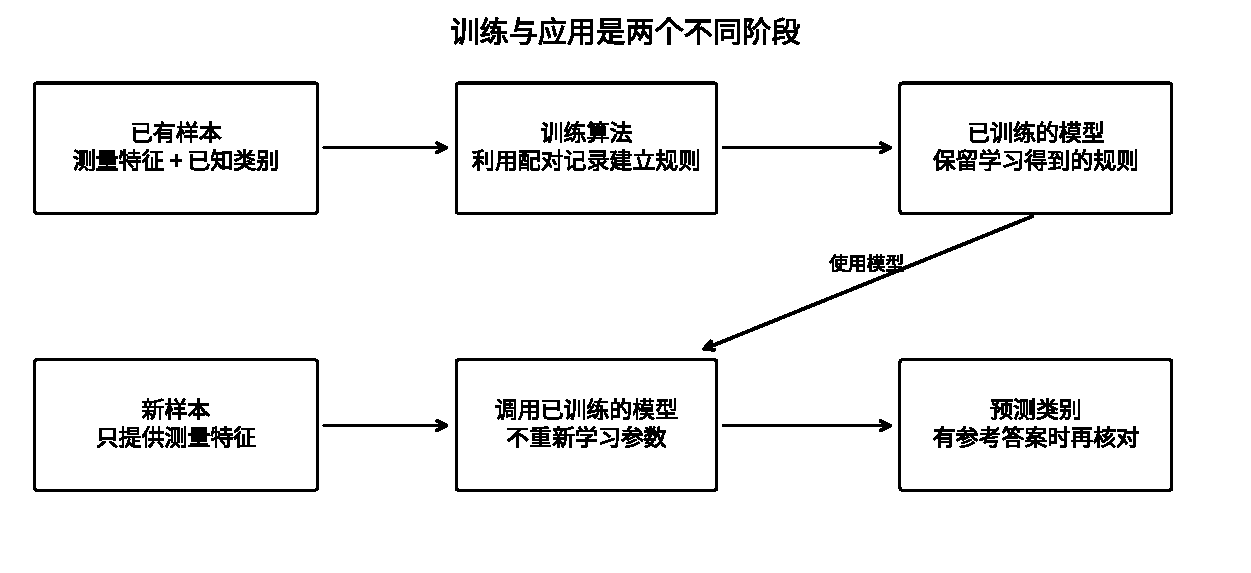
\includegraphics[width=0.92\linewidth]{figures/v2_supervised_flow.pdf}\caption{监督预测的学习与应用过程。标签在训练时提供学习依据，在评价时用于核对，不作为新样本预测的输入。}\label{fig:supervised-intro}\end{figure}

\subsection{学到规则和记住记录的区别}
设训练记录只有输入1、2、3，目标分别为3、5、7。规则甲保存三条记录，遇到完全相同的输入就返回对应目标；规则乙采用$\hat y=2x+1$。两者在已有记录上的预测相同，但对$x=2.5$，规则甲还需要额外规定如何处理，规则乙给出6。\textbf{训练数据上的一致表现，不足以唯一决定新输入上的行为。}

任何模型都包含关于新情况如何延续的假设。直线模型假设关系可以用固定斜率描述；近邻模型假设附近输入往往有相似目标；树模型假设可以通过若干阈值把输入空间分成较简单的区域。这类方法倾向在后面逐章解释。先认识到“数据告诉了什么”和“方法另外假设了什么”，才能理解为什么不存在对所有任务都最好的模型。

对于完全相同的输入却有不同目标的记录，模型也无法逐条区分。例如两条记录都是$x=2$，目标却是4和6，任何只看$x$的确定性规则都只能给出一个数。这可能来自测量噪声，也可能因为输入遗漏了重要条件。增加优化次数不会自动创造缺失的信息。第3章讨论怎样在这些目标之间折中，第16章讨论怎样区分噪声和可改善的模型误差。

\section{监督学习中的分类与回归}
\label{sec:supervised-definition}
\subsection{“监督”来自哪里}
\textbf{监督学习（supervised learning，也称有监督学习）是利用输入与已知目标成对出现的训练记录，学习从输入到目标的预测关系的一类方法。}“监督”指目标提供了学习所依据的信息，不是有人在程序运行时逐次指导，也不要求训练过程的每一步由人干预。

在花的例子中，程序同时获得尺寸与物种。它可以据此确定哪些特征组合有助于区分类别。我们已经知道部分答案，是为了学习以后怎样判断尚不知道答案的对象。训练时有目标与预测时目标未知并不矛盾，正是两个阶段的分工。

第8章的树模型根据类别组成选择划分规则；第6章的概率模型根据预测与目标之间的差异调整参数。它们都是监督学习，但内部学习过程不同。监督与否取决于训练使用的信息，不取决于是否调用某个软件函数，也不取决于是否使用梯度下降。

\subsection{分类：目标是类别}
\textbf{分类（classification）}是从一组已定义的类别中，为输入样本预测类别的任务。鸢尾花例子有三个可能物种，属于多分类。只区分“某物种”与“不是该物种”，就是二分类。类别之间可以有自然顺序，也可以没有；本书首先学习没有大小次序的类别识别。

一条记录的分类结果可能正确，也可能错误。后面的概率分类器还会输出对不同类别的支持程度，但此时先理解最基本的结果：预测物种与参考物种是否相同。

\subsection{回归：目标是数值}
\textbf{回归（regression）}是预测数值目标的任务，例如根据输入信号估计传感器输出。目标有大小和差值的意义，预测2.1与2.2的差别可以用相应单位解释。回归并不特指直线拟合，也不要求目标没有测量噪声。

本书采用\textbf{加州住房价值数据集（California Housing）}作为主要回归案例。每条记录对应一个人口普查街区组，即由若干住户构成的统计区域，而不是一套房屋。输入描述区域收入、住房、人口和位置；目标是该区域住房价值的中位数，数值以十万美元为单位。例如目标2.0表示20万美元。数据来自历史人口普查，用于学习建模，不是当前房价资料。具体字段在第5章逐项介绍\textsuperscript{[10]}。

如果模型给某区域预测2.2而参考目标为2.0，预测偏高0.2，即2万美元。这与把物种代码2预测为0不同：前者有可解释的数值差，后者是类别判断错误。任务类型要依据目标的含义判断，不能只看目标列是否存成数字。

\subsection{目标标签从哪里来，为什么也需要检查}
“已知目标”表示在当前数据中提供了可用于学习的参考，不表示参考一定无误。花的物种可以由人工鉴定给出，实验温度可以由参考仪器测量，天体类别可以由已有目录提供。每种获取方式都有适用条件和可能的误差。只有理解标签来源，才能知道模型实际上在学习什么。

例如，把已有分类程序的结果当作标签，新的模型首先是在学习复现该程序的判定，而不是直接获得了独立的物理真相。它可能具有速度或使用成本上的价值，但验证时应区分“与原程序一致”和“与独立可靠身份一致”。同样，把两种参考测量拼接成目标时，要检查单位、零点和量程是否一致。

\worked{同一测量量，可以导出不同任务}
考虑目标温度$T$。直接预测$T$是回归；把$T<0$定义为“低于冰点”、其余为“未低于冰点”，则变成二分类。二者都可以采用监督学习，但评价不同：回归关心偏差多少度，分类关心是否跨过指定界限。一次从$-0.1$预测成$0.1$摄氏度的误差很小，却可能改变类别；从30预测成32摄氏度误差更大，却未必改变这个二分类结果。

因此，不能脱离任务讨论一个误差是否严重。选择分类有时便于决策，但同时丢掉了数值差别；选择回归保留更多数值信息，却需要另外规定行动阈值。这是问题定义阶段应作出的判断，不是某个算法名称自动决定的。

\section{无监督学习中的聚类与降维}
\label{sec:unsupervised-definition}
\textbf{无监督学习（unsupervised learning）是在训练时不使用与样本配对的目标标签，而根据输入数据及事先规定的准则寻找结构或学习表示的一类方法。}它不是“没有任何规则地让程序随意探索”。分析者仍要决定使用哪些特征、怎样衡量相似、希望获得怎样的输出。

\subsection{同一数据，可以提出不同问题}
现在仍然使用花的四项尺寸，但把已知物种列暂时放在一旁，不交给算法。我们问：“哪些花在尺寸上相似，能否把它们组成几个群体？”根据相似关系形成群体的任务称为\textbf{聚类（clustering）}，所得群体称为\textbf{簇（cluster）}。

监督分类利用已定义的物种学习判断规则；聚类没有利用物种作为训练答案，而是依据输入的相似结构分组。因此，聚类中的“第0组”只是一组样本的编号，不天然对应物种代码0。即便分成三组，也不能直接断定它们就是三个物种。完成聚类后，可以把原有物种拿回来作对照，但这一步与训练时使用标签不同。

\subsection{降维：用较少变量重新表示样本}
每个样本的输入变量数称为其特征\textbf{维数}。四项尺寸给出四维表示。如果其中某些尺寸随花的整体大小一起改变，我们可能希望用少量组合变量概括主要变化。\textbf{降维（dimensionality reduction）}就是把数据变换为较少变量的表示，同时尽可能保留与所选目标有关的信息。

例如把四项尺寸变成两个组合值，便于在平面上画出样本分布。聚类回答“哪些样本应分在一起”，降维回答“怎样用更少的变量表示样本”，两者不能互换。第13章介绍一种具体的降维方法，第14章介绍聚类方法。

\begin{table}[htbp]\centering\small
\caption{学习方式与任务的区别。前者说明训练使用什么信息，后者说明希望输出什么。}
\begin{tabularx}{\linewidth}{p{0.16\linewidth}p{0.24\linewidth}XX}\toprule
学习方式&训练信息&任务例子&输出\\\midrule
监督学习&输入与对应目标&花的物种判断&一个已定义的类别\\
监督学习&输入与对应目标&区域住房价值预测&一个数值\\
无监督学习&不使用目标标签的输入&按花的尺寸寻找群体&群体划分\\
无监督学习&不使用目标标签的输入&压缩尺寸的表示&较少的组合变量\\\bottomrule
\end{tabularx}\end{table}

\subsection{没有标签时，怎样知道分析是否有用}
无监督学习没有提供唯一的参考答案，评价必须更紧密地联系用途。若希望压缩图像，可以检查重构图像丢失了哪些结构；若希望发现观测群体，可以检查相似分组在改变样本或测量误差后是否仍然存在，还可以检查没有参与分组的物理量是否呈现一致关系。

例如把花按尺寸分成两组，可以得到“大花与小花”的描述；分成三组可能更接近物种，也可能仍然混合。仅仅让算法返回更多组，会使每组内部更相似，却不代表科学解释更好。后面的聚类章节会明确区分“数学准则较好”和“符合我们关心的结构”。

已有标签仍然可以用作事后对照。关键是不要反复用这些标签调节无监督参数，然后仍声称标签从未影响分析。如果已经这样选择参数，整个流程就利用了标签信息。学习方式应按完整的信息流描述，而不是只按最后一个函数的名称分类。

\section{半监督、自监督与强化学习概览}
\textbf{半监督学习（semi-supervised learning）}同时利用少量有标签记录和较多没有标签的记录。例如，只辨认了一部分花的物种，但测量了更多花的尺寸；方法可以同时利用两部分数据。无标签记录怎样帮助学习，依赖额外假设，并非加入它们必然改善结果。

\textbf{自监督学习（self-supervised learning）}从数据自身构造学习目标。例如，遮住一幅图像的一部分，利用保留部分预测被遮住的内容。目标由已有数据产生，不需要人为逐条提供类别；但训练仍然有明确的预测任务和比较标准。

\textbf{强化学习（reinforcement learning）}研究行动者通过与环境交互，学习怎样行动以获得较大的长期累计奖励。行动者称为智能体，行动结果影响后续环境状态。例如一个简化的移动控制任务中，程序选择移动方向，环境返回位置和奖励；问题不仅是判断固定记录，还包括行动怎样影响以后能够获得的信息和结果。

这三类方法仅作概览，不是本课程的算法主线。它们可以在同一应用中组合，名称并不总是相互排斥。判断一段学习过程时，先看实际提供了什么信息、优化什么目标，再使用术语描述。

\section{一次完整机器学习任务的基本流程}
\subsection{先把过程讲清，再看软件}
对花的分类，一个完整入门实验可以按以下顺序进行：先明确输入为四项尺寸、目标为物种；检查记录与标签的对应；把一部分样本留作评价；用其余样本建立判断规则；只根据保留样本的尺寸预测物种；最后核对预测与参考物种，记录正确和错误的例子。代码应当能逐步对应这些操作。

本书使用\textbf{scikit-learn}，这是一个提供机器学习算法及数据处理、评价工具的Python软件包。在Python中导入它时使用模块名 \texttt{sklearn}；两种写法指向同一个工具。它与“监督学习”等方法概念不同，也与“鸢尾花数据”等具体资料不同。\texttt{load\_iris()} 是取得鸢尾花记录的函数，名称中的 \texttt{load} 表示读取；调用它不等于已经训练模型\textsuperscript{[26,30]}。

\begin{lstlisting}[caption={只读取已介绍的鸢尾花数据，不进行训练}]
from sklearn.datasets import load_iris
flowers = load_iris(as_frame=True)
X = flowers.data
y = flowers.target
print(X.shape, y.shape)
\end{lstlisting}

\noindent 上面代码中的输入对象在第2章将完整读入为表格。这里先用最少的读取语句区分“取得数据”和“根据数据学习”：创建变量 \texttt{flowers} 只是保存返回结果；\texttt{flowers.data} 是尺寸表。目标保存在 \texttt{flowers.target} 中，类别名称保存在 \texttt{flowers.target\_names} 中。表格操作及输出解释都在下一章展开，暂时不需要记忆所有接口。

\fig{ch01_workflow.pdf}{机器学习任务的完整流程概览。图中的模型选择是比较候选规则，最终评价是在规则确定后检查保留数据；具体操作将在第4章解释。}

\subsection{用一句完整的话描述你的任务}
一个可以开始实施的任务至少说清四件事：一条样本代表什么；预测时能获得哪些输入；希望输出什么；怎样检查输出是否有用。以花的例子为模板：“每条样本是一朵花；输入为四项尺寸；输出为物种；用训练时未使用的花检查物种判断是否正确。”

接触科学数据时，继续补充输入和目标的来源。例如，根据多波段亮度判断天体类别时，不同波段指不同波长范围内的亮度测量；参考类别可以来自更详细的光谱分析。此时就要区分用于预测的信息与用于提供参考答案的信息，而不是把表中每一列都投入模型。

\subsection{第一次完成一个小任务，不必立即理解所有算法}
下面的实验只使用已经认识的鸢尾花尺寸，先比较两个能读懂的判断规则。规则一对每朵花都报告训练部分中更常见的二分类结果；规则二规定“花瓣长度小于2.5厘米时报告setosa，否则报告非setosa”。后一阈值在这里是\emph{预先规定的教学规则}，不是通过本次验证数据寻找的最优值，也不作为正式的物种鉴定结论。

随书脚本先按固定随机种子保留30朵花作最终测试，不读取其结果；120朵开发样本中用90朵作训练、30朵作本次验证。训练部分确定多数类基线。实际运行中，验证30条里基线判断对20条，预先规定的长度规则判断对30条。这个结果说明该尺寸在这一小任务中有区分作用，但没有证明阈值2.5对所有新地区或新测量都有效。

\begin{lstlisting}[caption={把已有规则应用到新的输入，类别信息只用于最后核对}]
petal_length = X_val["petal length (cm)"].to_numpy()
predicted = petal_length < 2.5
reference = (y_val.to_numpy() == 0)
number_correct = (predicted == reference).sum()
print(number_correct, len(reference))
\end{lstlisting}
这段代码中的\texttt{X\_val}和\texttt{y\_val}来自随书完整实验的固定划分。比较发生在预测之后：条件判断只读取花瓣长度，参考物种没有进入判断条件。第4章解释划分方法，第8章把人工规定阈值改成由训练数据选择阈值。这样，已有经验规则、简单基线与学习算法之间的联系就清楚了。

\subsection{检查本章是否真正学会}
读完本章，应该能把任一案例分成三层：现实对象是什么；为完成任务把它表示成哪些数字；程序根据这些数字做什么。没有读懂第一层时，不应急于讨论第三层的算法参数。能够在纸上画出训练与预测的信息流，比提前记住十个模型缩写更重要。

\chapterpractice{先读表\ref{tab:iris-records}，逐项说出样本、输入与目标。再用同一数据描述分类和聚类两个任务，明确哪一步使用类别信息。最后任选一个熟悉的实验或天文问题，写出样本、输入、预期输出及一个检查结果的方法；这一任务只要求定义问题，不要求提前实现算法。}
\chapterexercise
\begin{enumerate}
\item 一张表有150行、4列尺寸和1列物种。用于物种分类的特征矩阵有几行几列？为什么不把物种列同时作为输入？
\item 训练时已经知道花的物种，为什么仍然需要学习分类规则？训练、预测、评价各使用什么信息？
\item 把三个物种编码为0、1、2，是否就变成了回归问题？请说明目标含义与存储形式的区别。
\item 同一批尺寸记录，怎样分别用于分类和聚类？聚类组号为什么不能直接当作物种编号？
\item 在实验记录中，一行是一件材料还是一次测量，为什么需要先说明？写出一个完整的任务定义。
\end{enumerate}

\section*{深化练习与方法检验}
本组题强调解释、计算与验证；D编号在本章内独立计数。计算题应写出所用定义和中间步骤，实验题保留实际输出，包括不支持预期的结果。
\begin{enumerate}[label=D\arabic*.]
\item 某表记录同一传感器在不同输入电压下的读数。任务甲根据输入电压估计输出电压，任务乙根据输出曲线判断传感器是否故障。两者的样本单位、输入和目标是否必然相同？各写一份没有信息泄漏的任务定义。
\item 两个对象的全部输入完全相同，但参考类别不同。一个确定性的分类模型能否同时把两条记录都分对？这说明提高算法复杂度能够解决什么、不能解决什么？
\item 算法先把图像的一部分遮住，学习预测被遮住的像素，再利用少量物种标签进行分类。分别说明两个阶段的学习目标、目标来源，以及两个阶段是否都可以有数值损失。
\item 把鸢尾花物种标签随机打乱后，仍能得到一张格式正确的数据表。此时数据形状检查与科学含义检查分别能发现什么？设计一个不需要复杂算法的核对步骤。
\end{enumerate}

\chapter{数据表示、探索与准备}
\label{chap:data}
\chaptergoal{能够读懂一张样本表，说明每列的含义与用途；使用Pandas读取、选择和检查数据；解释缺失值、类别编码和标准化；区分从训练数据确定处理规则与把规则应用到新数据。}

上一章已经认识了花的尺寸与物种记录。本章把“读懂数据”落实为可以执行的操作。重点不是记忆许多命令，而是让每一步都有明确对象：读入什么、改变什么、保留什么，以及处理后的表是否仍然对应原来的样本。

本章使用两个已经分工明确的例子：鸢尾花数据用于练习表格与散点图；接下来介绍的葡萄酒化学分析数据用于观察多种测量量的尺度。先理解记录的含义，再学习读取函数。

\section{从科学记录到样本表}
\subsection{数据表不只是一个数字矩阵}
\textbf{样本表}把记录按行排列，把字段按列排列。字段是有名称的一项记录内容，可以是测量值、类别、编号或质量说明。\textbf{字段字典}则是解释字段的附表，至少说明名称、含义、单位、数据类型和本次任务中的用途。它相当于实验记录本中对各列的说明，不能由程序自动猜出。

\textbf{CSV}是“逗号分隔值”（comma-separated values）的缩写，是一种用文本保存表格的文件形式。通常第一行写列名，后续每行写一条记录，相邻数值以逗号分隔。例如一份人为构造的长度测量表可以写为：
\begin{lstlisting}[language={},caption={用于理解CSV格式的人工三行示例，长度单位为厘米}]
record_id,length_cm,width_cm,class_id
A01,5.1,3.5,0
A02,7.0,3.2,1
A03,6.3,3.3,2
\end{lstlisting}
这只是格式示例，不能当作完整的鸢尾花数据。CSV文件可以保存数字和文字，但文件后缀不会自动告诉我们单位、物种映射或测量方法。因此，表格和字段字典需要一起保存。

\subsection{葡萄酒化学分析数据是什么}
\label{sec:wine-intro}
现在考虑第二个问题：\textbf{能否根据葡萄酒的化学测量指标，区分它来自三种葡萄栽培品种中的哪一种？}本例采用\textbf{葡萄酒化学分析数据集（Wine dataset，简称葡萄酒数据）}。Wine是数据集名称，不是模型。数据由同一意大利地区、三种葡萄栽培品种酿成的葡萄酒样本的分析结果组成，共178条记录，每条有13个数值特征。任务是类别识别，不是品质评分或价格预测\textsuperscript{[2,27]}。

表\ref{tab:wine-fields}列出全部字段。原始来源的变量表未系统给出各字段的单位，本书保留这一限制，不根据日常常识自行补成百分比或浓度单位。我们仍能比较数据中的数值尺度，但不能把标准化实验写成未经核验的化学计量结论。
\begin{longtable}{p{0.40\linewidth}p{0.49\linewidth}}
\caption{葡萄酒数据的13项特征。英文名对应程序列名；单位以原来源说明为准，此处未擅自补写。}\label{tab:wine-fields}\\
\toprule 程序字段&中文含义\\\midrule\endfirsthead
\toprule 程序字段&中文含义\\\midrule\endhead
\texttt{alcohol}&酒精相关测量指标\\
\texttt{malic\_acid}&苹果酸指标\\
\texttt{ash}&灰分指标\\
\texttt{alcalinity\_of\_ash}&灰分碱度指标（保留源字段拼写）\\
\texttt{magnesium}&镁指标\\
\texttt{total\_phenols}&总酚指标\\
\texttt{flavanoids}&类黄酮指标（保留源字段拼写）\\
\texttt{nonflavanoid\_phenols}&非类黄酮酚指标\\
\texttt{proanthocyanins}&原花青素指标\\
\texttt{color\_intensity}&颜色强度\\
\texttt{hue}&色调指标\\
\texttt{od280/od315\_of\_diluted\_wines}&稀释酒样在280与315纳米处的光密度比值\\
\texttt{proline}&脯氨酸指标\\\bottomrule
\end{longtable}

三个类别在sklearn中编码为0、1、2，对应59、71、48条记录。原UCI文件使用1、2、3，数字偏移不改变类别本身，但合并资料时必须核对映射\textsuperscript{[2,27]}。类别编号没有高低品质的含义。学本例不要求化学专业知识；至少要知道每条记录是酒样分析、各列是不同测量指标、目标是来源类别。

下面再读三条实际记录。表\ref{tab:wine-records}只选取三个测量字段，完整输入仍是13项。第一行表示一份酒样的酒精指标为14.23、镁指标为127、颜色强度为5.64，类别为0；它不是“价值14.23”或“质量为0”。在没有核实原测量单位之前，只按源数值与明确的字段含义读取。
\begin{table}[htbp]\centering\small
\caption{葡萄酒数据的三条实际记录摘录。行号为零起始位置，类别列不是输入；数值按来源保留，未擅加单位。}\label{tab:wine-records}
\begin{tabular}{rrrrr}\toprule
行号&酒精指标&镁指标&颜色强度&来源类别\\\midrule
0&14.23&127&5.64&0\\
59&12.37&88&1.95&1\\
130&12.86&122&4.10&2\\\bottomrule
\end{tabular}\end{table}

\subsection{宽表、长表和样本单位的选择}
同一组物理测量可以有不同表形。若每个天体在五个波段各测一次，可以用一行表示一个天体、五列表示五个波段；也可以用五行表示五次测量，增加波段名称列。前者常称宽表，后者常称长表。两者存储的信息可能相近，但普通表格模型的样本定义不同。

在预测天体类别时，五个波段通常共同描述同一天体，把它们作为五个独立样本会丢失波段之间的关系。若研究的是随时间变化的亮度，时间和对象标识又必须保留。选择表形应从任务出发，不宜为了适应某个函数随意改变样本单位。

\worked{合并表格时，顺序不能代替身份}
输入表按A、B、C存储三个对象，标签表按C、A、B存储目标30、10、20。直接把目标列贴到输入表末尾，会得到A对应30、B对应10、C对应20，三行都错了。按标识合并，才得到A对应10、B对应20、C对应30。程序如下：
\begin{lstlisting}
features = pd.DataFrame({"id": ["A", "B", "C"], "x": [1., 2., 3.]})
labels = pd.DataFrame({"id": ["C", "A", "B"], "target": [30., 10., 20.]})
joined = features.merge(labels, on="id", validate="one_to_one")
assert joined["target"].tolist() == [10., 20., 30.]
\end{lstlisting}
\texttt{validate}检查合并键是否满足一对一关系。若一个对象确实有多次观测，需要明确使用一对多结构，不能简单删除重复键。合并前后都应记录行数及没有匹配成功的对象数。行数增加可能来自预期的多次观测，也可能来自错误的多对多连接。

标识字段要无损保存。很长的整数标识不宜先转成浮点数再转回整数；浮点数的有限精度可能改变末尾数字。可以根据来源使用64位整数、可空整数或字符串。标识并不参与数值距离，所以保存为字符串通常不会妨碍建模。

\section{使用Pandas与sklearn读取数据}
\subsection{表格对象与软件工具}
\textbf{Pandas}是Python中的表格处理软件包。它提供的\textbf{DataFrame}可以理解为带行索引和列名的二维表；\textbf{Series}是带索引的一列数据。索引用来定位表中行，并不自动等于科学对象编号。代码常写 \texttt{import pandas as pd}，其中 \texttt{pd} 只是约定俗成的简称。

scikit-learn负责提供模型和相关工具，其中的 \texttt{load\_wine()} 用于读取刚介绍的葡萄酒数据。设置 \texttt{as\_frame=True}，表示希望把主要数据以Pandas表格形式返回。返回对象同时包含特征、目标和说明，这几部分需要区分。
\begin{lstlisting}[caption={先读取葡萄酒数据，再检查表格角色}]
from sklearn.datasets import load_wine
import pandas as pd

wine = load_wine(as_frame=True)
X = wine.data.copy()
y = wine.target.copy()
table = X.assign(class_id=y)
print(X.shape)
print(table[["alcohol", "magnesium", "color_intensity", "class_id"]].head(3))
print(table.groupby("class_id").size())
\end{lstlisting}

\texttt{X.shape} 返回 \texttt{(178, 13)}，表示178条样本、13列输入。\texttt{table} 在输入表上附加类别，因此有14列；调用 \texttt{assign} 不会把原输入表里的列自动变成目标。\texttt{head(3)} 只显示前三行，\texttt{groupby("class\_id").size()} 按类别统计行数。\texttt{copy()} 创建可单独修改的数据副本，避免在探索中无意改变原对象。

\subsection{CSV与DataFrame之间的转换}
\begin{lstlisting}[caption={把同一数据保存为CSV后重新读入}]
table.to_csv("wine_table.csv", index=False)
reloaded = pd.read_csv("wine_table.csv")
X_again = reloaded.drop(columns="class_id")
y_again = reloaded["class_id"]
print(X_again.shape, y_again.shape)
\end{lstlisting}
\texttt{index=False} 表示不把Pandas行索引额外写成一列。\texttt{drop(columns=...)} 在这里移除目标列，得到输入；方括号选择目标列。读入后要检查列名和顺序，尤其不能因为CSV多出一个索引列，就把它当作第14个测量特征。

\subsection{读取成功之后，先做三个一致性检查}
程序没有报错只说明文件在语法上可读取，并不说明内容符合任务。首先检查行数和列名；其次检查各列的数据类型与缺失数量；最后抽看几条记录，按字段字典解释其含义。训练代码应在这些检查通过之后运行。

例如长度列可能被读成字符串，因为其中混有“未测得”文字；目标列可能包含前后空格，使本应相同的标签被认为是不同类别；保存CSV时附带的旧行索引可能成为一列\texttt{Unnamed: 0}。这些情况不能靠模型自动纠正。将字符串转成数字时，如果允许无法转换的内容变为缺失值，还应统计新增了多少缺失，避免悄悄丢失数据。

\begin{lstlisting}[caption={读取一个已说明字段含义的CSV后检查数据}]
df = pd.read_csv(path)
print(df.shape)
print(df.dtypes)
print(df.isna().sum())
required = {"record_id", "target"}
if not required.issubset(df.columns):
    raise ValueError("Required fields are missing")
if df["record_id"].duplicated().any():
    raise ValueError("Record IDs are not unique")
\end{lstlisting}
实际数据的必需字段名应按对应字典修改。检查规则不应该机械复制到不同任务；一个时间序列表的对象标识可以重复，但记录标识仍应能够区分每次测量。明确报错比继续训练后得到难以解释的结果更安全。

\section{数据划分与预处理的信息边界}
\subsection{为什么先把部分记录留出来}
在改变数值之前，先回忆第1章的要求：要检查模型对未参与学习的对象是否有效。为此，把可用于反复试验的一部分称为\textbf{开发数据}，另留一部分供最后检查，称为\textbf{最终测试数据}或保留数据。开发数据中又可以区分用于学习的训练部分和用于比较方案的验证部分，第4章系统解释。

\textbf{预处理（preprocessing）}是模型训练之前对数据表示进行准备的过程，例如填补缺失值、把类别写成可用的数值列、调整特征尺度。有些操作只执行固定规则，有些则要从数据估计一个数。计算填补均值、计算标准差都属于后者：虽然没有训练分类器，这些操作也已经从数据获得了信息。

\begin{lstlisting}[caption={先确定开发部分和最终保留部分}]
from sklearn.model_selection import train_test_split
X_dev, X_hold, y_dev, y_hold = train_test_split(
    X, y, test_size=0.2, stratify=y, random_state=42
)
print(len(X_dev), len(X_hold))
\end{lstlisting}
这里 \texttt{test\_size=0.2} 指约20\%的记录留出；\texttt{stratify=y} 尽量保持两部分的类别比例。

\noindent 参数\texttt{random\_state=42} 固定一次随机拆分，便于重复。42没有特殊科学意义，换其他整数也可形成合法拆分。代码把同一行的输入与目标一起划分，不能先分别打乱二者。

\subsection{固定处理规则，再用于新记录}
假设训练部分某列有三个有效值10、12、14，我们选择用其均值12填补缺失。验证样本如果这一列缺失，也应填入12，而不是先把验证样本的其他数值合并进去重新计算均值。因为要模拟的正是“学习完规则以后遇到新记录”。

把用于检查的数据提前参与规则确定，称为\textbf{数据泄漏（data leakage）}的一种情形。先知道正常操作，再检查是否越界：固定规则依据训练范围确定，验证和测试只应用该规则。这里只建立这个原则，第4章把它推广到模型比较和交叉验证。

\subsection{为什么无标签的预处理也会使用数据的信息}
标准化虽然不读取目标，却读取特征分布。假设训练测量为0、1，未来验证测量为100。只用训练数据中心化时，均值是0.5，新值100位于训练中心很远处；把三条合起来计算时，均值约33.667，训练表示已经受到未来极端值影响。模型在真正部署前通常拿不到未来整批数据，因而后一操作改变了所模拟的信息条件。

有时这种改变对某个算法的最终分数影响很小，甚至没有影响，但不能据此认为所有预处理越界都无害。特征筛选、降维和缺失模式估计可能产生更明显影响。正确规则是：凡是从数据中学习出来的处理参数，都应依据当前训练范围确定。固定的单位换算，例如厘米换米，不需要估计总体参数，通常可以在划分前完成，但也要保存换算说明。

\worked{中位数填补的信息来源}
训练列为$(1,2,\text{缺失},4)$，训练非缺失中位数为2，所以训练缺失值填成2。后来验证列有$(100,\text{缺失})$，验证缺失也填2，而不是根据100重新决定填100。这个处理没有恢复真实未知值，只是保证模型接收到由训练规则规定的数值。模型以后是否受这种近似影响，需要通过相同流程的验证来判断。

交叉验证时，“当前训练范围”会随折改变。因此不能先在全部开发数据上填补和标准化，再把变换后的矩阵交给交叉验证。第4章的流水线将每轮的拟合重新放在正确位置。这里先理解信息来源，再使用自动化接口。

\section{特征矩阵、目标变量与数据类型}
\subsection{形状与逐行对应}
若选择葡萄酒数据的两个字段，可写 \texttt{X[["alcohol", "magnesium"]]}，得到178行、2列的表。若只使用一个字段，双层方括号仍返回一列表格，形状为 $(178,1)$；单层方括号一般返回一维Series。两者数值可以相同，但传给接口时形状不同。

\begin{lstlisting}[caption={用表格列选择理解一个特征和一个样本}]
one_feature = X[["alcohol"]]
one_sample = X.iloc[[0]]
print(one_feature.shape)  # (178, 1)
print(one_sample.shape)   # (1, 13)
\end{lstlisting}
\texttt{iloc}按整数位置选行，双层方括号保留二维结构。第一种表示178个样本各一个特征，第二种表示一个样本有13个特征，不能互换。目标序列的第 $i$ 项必须对应特征表第 $i$ 行。

\subsection{存储类型与科学含义}
\textbf{数据类型}说明计算机如何保存和运算某列，例如整数、浮点数、布尔值或文字。浮点数用于近似表示带小数的数值，布尔值通常为真或假。\texttt{dtypes}可检查各列类型，但“整数”不等于“具有可比较大小的物理量”：物种代码也是整数。

编号、分组字段、质量字段、输入、目标应分别记录角色。对于重复观测，一列对象编号可用于把同一天体的记录放在同一组，而不作为预测特征。特别长的整数编号不宜转换为浮点数，因为浮点表示可能不能精确保留每一个末位数字；可以保持整数或字符串。

\subsection{列顺序、形状与运算方向}
矩阵$X\in\mathbb R^{n\times p}$把样本放在行、特征放在列。对每列求均值使用沿样本方向的汇总；对每行求向量长度则是在特征方向汇总。以三行两列$X=((1,10),(2,20),(3,30))$为例，列均值是$(2,20)$，行均值是$(5.5,11,16.5)$，两者回答不同问题。

\texttt{axis=0}和\texttt{axis=1}容易被记忆口诀弄混，最好先问输出应当有几个数。每个特征一个中心值，应得到$p$个数；每条记录一个距离，应得到$n$个数。代码运行成功并不保证轴选对，因为错误方向也可能得到合法数组。

一个样本仍需要二维输入：\texttt{X.iloc[[0]]}保留一行多列，而\texttt{X.iloc[0]}通常返回一维序列。向模型提交多个特征时，应保存列名称及顺序。即使两份表包含同样的数，把酒精列与镁列互换也会改变模型含义。不同数据源合并后应显式选择约定列序，而不是依赖文件原始列顺序。

\subsection{有序类别和无序类别}
有序类别具有大小关系，例如人工规定的低、中、高等级；无序类别如仪器A、B、C，没有自然的数值间距。给有序类别编码0、1、2，也只是规定了顺序，并不自动证明从低到中的变化等于从中到高。模型怎样处理这一编码，需要与任务假设一起考虑。

目标类别的数字编码用于表示身份，输入类别的编码则影响算法如何计算关系。两个问题应分开处理。对于输入仪器型号，独热编码允许模型为每种型号使用独立的系数；对于目标物种，分类器会把0、1、2看作不同类别。不要把两种编码都称为“把文字变数字”而忽略其统计作用。

\section{训练数据的统计描述与可视化}
\subsection{用一个小例子理解统计量}
考虑人为给出的四个读数1、2、3、10。\textbf{均值}是总和除以记录数，为4；\textbf{中位数}是排序后处于中间位置的值，偶数个记录时取中间两项平均，因此为2.5。读数10把均值明显拉高，却没有同样幅度地改变中位数。这说明“典型值”不是唯一的计算定义。

\textbf{方差}描述数值围绕均值的平方偏离；\textbf{标准差}是方差的平方根，与原量具有相同单位。\textbf{分位数}表示排序后某个比例位置的值，例如四分位数帮助观察中间一半记录的范围。\texttt{describe()}提供这些摘要，但具体分位数插值与方差分母应以所用函数为准；手算比较时要采用一致约定。

\begin{lstlisting}[caption={检查开发数据，不把汇总数字当作背景解释的替代}]
print(X_dev.dtypes)
print(X_dev.isna().sum())
print(X_dev.describe().T[["mean", "std", "min", "max"]])
\end{lstlisting}
\texttt{isna()}把缺失位置标为真，按列 \texttt{sum()} 得到缺失数量。一个变量的最小值、最大值异常，并不自动说明该记录错误；先检查单位、录入、筛选规则和真实的对象差异。

\subsection{先学会读坐标再解释图形}
\textbf{散点图}把每条记录画成一个点，横纵坐标分别是两个字段。图\ref{fig:iris-data}展示鸢尾花的两项尺寸：看一个点，就是同时读这朵花的两个测量值。点的类别标记来自已知物种，不是由图自动推断的。多个点形成带状结构，可能说明两个尺寸一起变化；仅凭散点图不能判定其中一个造成另一个。
\begin{figure}[htbp]\centering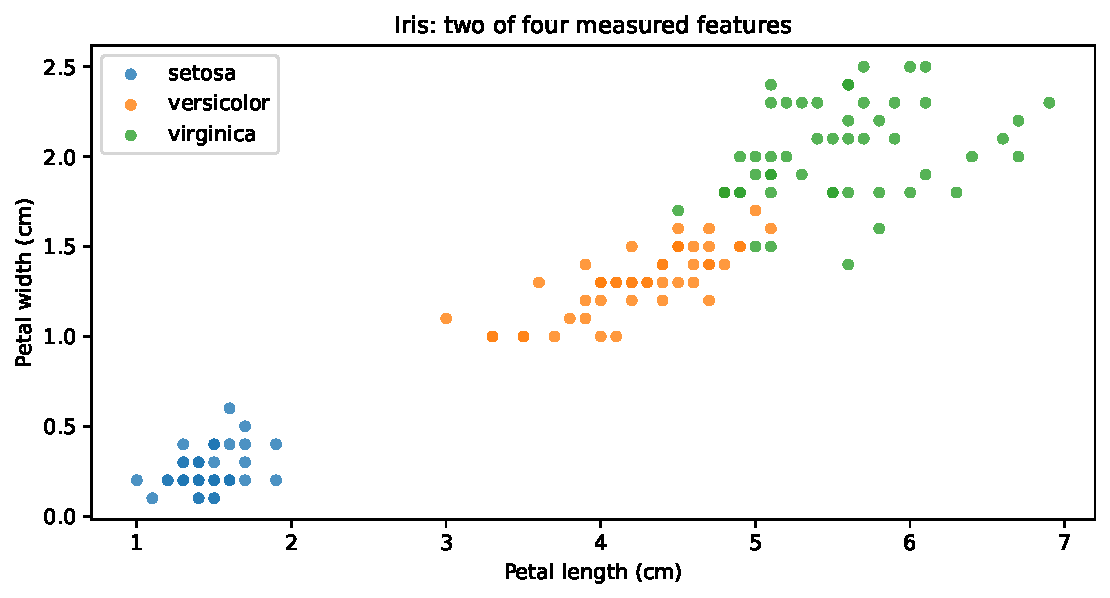
\includegraphics[width=0.83\linewidth]{figures/ch02_iris_scatter.pdf}\caption{鸢尾花两个尺寸的散点图。横纵坐标仅显示四项输入中的两项，不代表已经完成全特征分类。}\label{fig:iris-data}\end{figure}

\textbf{直方图}把一个变量的取值范围分为若干区间，统计各区间记录数，用于观察分布是否集中、偏斜或存在多个峰。画图时应标字段、单位和样本范围，不能只写 \texttt{x}、\texttt{y} 却让读者猜其含义。

\subsection{用分位数和散点图寻找值得追问的记录}
平均值容易受到极端记录影响，中位数表示排序后的中间位置，分位数描述分布的不同部分。四分位距是第75百分位与第25百分位之差，常用于概括中间一半数据的跨度。它们是描述工具，不是自动清洗规则。

例如某个长度列大多数记录在1到10厘米之间，却有一条为500。至少存在三种解释：对象确实很大、该行使用毫米、录入发生错误。只凭“离均值很远”不能确定是哪一种。应回到单位、原始记录和其他相关字段，再决定保留、转换、标记或排除。自动删除极端记录可能恰好删除最值得研究的对象。

相关系数描述两个变量的线性共同变化。两个变量即使相关系数接近零，也可能存在弯曲关系。例如对对称分布的$x$，$y=x^2$可能没有线性相关，却完全由$x$确定。散点图能够补充单个汇总数字看不到的形状。后面线性模型的残差图也采用相同思路：先看模式，再考虑是否需要变换特征或更换模型。

\subsection{缺失和质量字段也有分布}
缺失不是纯粹的软件问题。弱信号可能更难测到某个波段，极端实验条件可能更容易失败。若只保留全部测量齐全的样本，最终研究对象的范围可能发生改变。应记录每一步筛选前后的样本数量，并比较保留与排除记录已有字段的分布。

这不要求初学者立刻掌握复杂的缺失机制模型，但必须学会提出问题：缺失是否与类别、信号强弱或设备条件有关？只有在了解这些关系后，才知道均值填补和删行分别可能造成什么影响。第16章会把这种检查与模型的适用范围联系起来。

\section{缺失值处理与类别编码}
\subsection{缺失不是数值零}
\textbf{缺失值}表示某项记录没有可用值，可能因为未测量、记录丢失或质量不合格。在Pandas中，数值缺失常以 \texttt{NaN} 表示。零是一个具体数值，不能未经解释就代替缺失。原始葡萄酒数据没有缺失；本章Notebook人工遮去少量值，只是为了演示处理步骤，并保留未改动的原表。

\textbf{填补（imputation）}按规定规则为缺失位置提供用于后续计算的替代值。假设训练列为1、缺失、3、8，用已有值的中位数3填补，就得到1、3、3、8。这个3不是恢复出的真实测量，只是一个处理规则的结果。规则所需的中位数从训练数据确定，再应用于验证和测试。

下面同时使用\textbf{NumPy}，这是Python的数值数组工具包，程序中通常简写为\texttt{np}。\textbf{数组}是按固定形状排列的一组数，\texttt{np.nan}表示缺失数值，而不是零。示例先人为制造一个缺失值，用来核对填补步骤，不代表原始葡萄酒数据已有缺失。

\begin{lstlisting}[caption={先手算，再用软件核对中位数填补}]
import numpy as np
from sklearn.impute import SimpleImputer
values = np.array([[1.0], [np.nan], [3.0], [8.0]])
imputer = SimpleImputer(strategy="median")
print(imputer.fit_transform(values).ravel())
print(imputer.statistics_)  # learned replacement: 3
\end{lstlisting}

\subsection{输入类别的独热编码}
假设另一个人工测量表记录仪器类型A、B、C，它们没有数值大小。可以把仪器类型改写为三列：A对应 $(1,0,0)$，B对应 $(0,1,0)$，C对应 $(0,0,1)$。这种表示称为\textbf{独热编码（one-hot encoding）}，每列表示是否属于某类别。它避免把A、B、C直接写成0、1、2后引入并不存在的等间距关系。

这里处理的是\textbf{输入中的类别型特征}，与目标类别用0、1、2保存是不同问题。编码规则也要保存，以便新数据使用相同列顺序。遇到训练时没有出现的仪器类型，需要明确处理办法，而不是临时改动输入列数。

\subsection{填补会改变分布，缺失指示可以保留部分信息}
假设一列四个可用训练值为0、2、4、6，另有四个缺失。用均值3填补后，新增的四个数都落在中心，样本的离散程度变小了。模型看见的表比原始测量更集中，但这并不表示实验精度提高。这是填补规则引入的结构。

可以另外增加一个“原来是否缺失”的二值字段，让模型知道哪些数来自测量、哪些来自填补。这种缺失指示并不一定改善预测，也不能修复偏差，但它避免把估计值与真实测量完全混为一谈。使用时应检查部署数据是否具有类似缺失机制，否则模型可能学到一条只适用于旧设备的数据获取规则。

\subsection{训练中没有见过的类别}
训练只有仪器A和B，应用中出现C时，编码器应按预先规定的策略处理。直接临时增加一列会改变后续模型输入维数；把C强行改成A又会伪造含义。可以使用允许未知类别的编码器、专门的其他类别，或拒绝给出预测并要求补充标定。采取哪一种策略取决于任务，而不是统一越宽松越好。

下面的编码器把已知类别学成固定列，并让未知类别在这些列上为零。零向量仅表示“这些已知指示列都不成立”，不表示新仪器与旧仪器行为相同。后面的线性模型还会叠加截距，所以未知类别仍可能产生一个数值预测，但这个数值的可靠性需要单独检查。
\begin{lstlisting}
from sklearn.preprocessing import OneHotEncoder
encoder = OneHotEncoder(handle_unknown="ignore", sparse_output=False)
encoded_train = encoder.fit_transform([["A"], ["B"], ["A"]])
encoded_new = encoder.transform([["C"]])
print(encoder.categories_, encoded_new)
\end{lstlisting}

\section{特征尺度、标准化与处理流程}
\label{sec:standardization}
\subsection{标准化究竟改变什么}
\textbf{尺度}指变量数值变化的量级。葡萄酒的某些指标取值接近个位数，另一些可达到数百甚至上千。如果算法依据数值差计算距离，较大的尺度可能支配结果。长度由米换成毫米也会放大数字，却没有改变对象本身，这提示我们要区分测量含义和数值表示。

\textbf{标准化（standardization）}在本书指用训练均值 $\mu$ 减去中心，再除以训练标准差 $s$：
\[
z=\frac{x-\mu}{s}.
\]
$z$表示某个值高于或低于训练均值多少个标准差。对训练值1、2、3，采用分母为3的方差约定，$\mu=2$，$s=\sqrt{2/3}\approx0.8165$，变换后约为 $-1.225,0,1.225$。一个后来出现的值4应使用同一个均值和标准差，得到约2.449，不能单独对这个新值重新计算中心和尺度。\texttt{StandardScaler}使用的方差分母为训练记录数，其零方差列另有安全处理\textsuperscript{[31]}。

\fig{ch02_wine_scales.pdf}{葡萄酒部分测量字段在原始与标准化表示中的尺度。标准化使单位尺度可比较，不保证任意分类方法的效果都会提高。}

\subsection{fit与transform分别完成什么}
\begin{lstlisting}[caption={把学习尺度和应用尺度分成两步}]
from sklearn.preprocessing import StandardScaler
scaler = StandardScaler()
scaler.fit(X_dev)
X_dev_scaled = scaler.transform(X_dev)
# Do not fit the scaler again on the held-out records.
X_hold_scaled = scaler.transform(X_hold)
print(scaler.mean_[:3], scaler.scale_[:3])
\end{lstlisting}
对这个变换器，\texttt{fit}只从输入计算均值和尺度，没有学习类别；\texttt{transform}按已保存的规则改变数值。\texttt{fit\_transform}把两步合并，适用于学习规则的训练数据，不应在测试数据上重新调用来得到另一套尺度。

\textbf{流水线（Pipeline）}把若干处理步骤按顺序连起来。例如“填补缺失—标准化—分类模型”是一个整体：训练时前面的步骤学习处理规则，后面的模型学习预测规则；预测时所有步骤应用已经保存的规则。第4章将用它在每次验证中重新建立训练流程。先理解这里的手动两步，再理解流水线为什么能减少漏做或错用步骤的风险。

\textbf{归一化}在不同资料中含义不完全一致，有时指缩放到固定区间，有时指把整个样本向量缩放为固定长度。本书不把它作为所有尺度处理的统称；报告中写明实际公式或所用变换器。标准化也不能修复错误标签或补全测量信息，它只改变数值表示。

\subsection{尺度变换怎样改变距离和参数含义}
考虑两维输入：长度以米计，质量以千克计。两点的欧氏距离平方写成$(\Delta x_1)^2+(\Delta x_2)^2$，把长度换成毫米后，第一项放大一百万倍。物理对象没有改变，但默认距离的相对权重改变了。标准化相当于先给每个方向规定一个比较尺度，再计算距离，因此需要与“相似”的含义一起考虑。

对线性预测$\hat y=b+wz$，若$z=(x-\mu)/s$，则
\[
\hat y=\left(b-\frac{w\mu}{s}\right)+\frac{w}{s}x.
\]
所以标准化坐标中的系数不是原始单位下的斜率。可以通过这个代换把参数还原，不必把变换后的模型看成无法解释的对象。若有多个特征，对每列分别换算并把所有截距修正加总即可。这个关系会在第5章系数解释中使用。

标准化不能保证分布变成正态分布。一个明显偏斜、有两个峰或含极端值的分布，减均值除标准差以后仍可能保留相同形状。它也不等于把所有值限制在$[0,1]$，验证记录完全可以超过训练均值很多个标准差。\textbf{处理公式决定它改变什么，名称不能代替公式。}

\subsection{一次可以复核的数据准备实验}
随书实验在葡萄酒训练数据中，人工遮去8个酒精测量值，并保存原位置清单。它先用训练中位数填补，再用训练均值和标准差缩放，最后把同一流程应用到验证数据。实验没有修改原始公开数据文件，也没有宣称这些缺失来自真实采样。

训练变换后的各列均值接近零，这是标准化的定义结果；验证列均值通常不等于零，这是合理现象，因为验证记录与训练记录不同。不要为了让验证均值也恰好为零，再在验证数据上拟合一个新的缩放器。检查时应核对处理规则是否一致，而不是要求所有数据都出现同样的统计数字。

\subsection{怎样组织不同类型字段的处理}
实际表格可能同时含有数值字段与类别字段。数值字段可以依次填补、缩放，类别字段可以填补后独热编码。\texttt{ColumnTransformer}按列把这些不同流程并行组织起来；\texttt{Pipeline}再把合并后的特征送给模型。两者不是额外的机器学习算法，而是保存数据处理顺序和字段角色的工具。

初次练习时可以手动完成一列变换，等每一步含义清楚后再组合。最终提交应保存字段顺序、已学习的中位数或类别表、缩放参数及模型。只保存最后一组模型系数，往往不足以在新数据上重现同样的预测。

\chapterpractice{用葡萄酒数据完成读取、保存CSV、重新读入和字段角色检查；手算本章的中位数填补和标准化例子，再用代码核对；在开发数据上计算字段统计量和绘图；说明保留数据为什么只应用处理规则。算法性能比较留到第4章以后。}
\chapterexercise
\begin{enumerate}
\item 葡萄酒数据中，一行表示什么？13项输入与类别列各承担什么角色？为什么这不是品质评分任务？
\item \texttt{X[["alcohol"]]}与\texttt{X.iloc[[0]]}在形状和含义上有什么不同？
\item 对训练值2、4、6，采用分母为3的方差进行标准化；再将新值8按训练规则变换。写出各步结果。
\item 缺失值与零有什么不同？中位数填补能否恢复没有测到的真实数值？
\item 为什么在测试部分重新调用\texttt{fit\_transform}可能改变模型实际看到的特征含义？
\end{enumerate}

\section*{深化练习与方法检验}
本组题强调解释、计算与验证；D编号在本章内独立计数。计算题应写出所用定义和中间步骤，实验题保留实际输出，包括不支持预期的结果。
\begin{enumerate}[label=D\arabic*.]
\item 主表有对象A、B两行，辅助表中A出现三次、B出现一次。按对象编号合并后有几行？怎样检验原本期望的一对一关系，为什么直接在合并后随机拆行可能产生问题？
\item 对训练列 $(1,3,5)$ 用分母为3的方差标准化，并把新值7变换到同一坐标。再说明：把训练值与新值合并后重新计算均值，得到的是不是同一个预测流程？
\item 一个输入字段缺失时，仪器往往处于低信噪比状态。只用中位数填补可能遗漏什么信息？设计一种保留“是否缺失”的表示，并说明它可能在哪种部署变化下失效。
\item 长度从米改为毫米后，原始欧氏距离、标准化后的距离、按单特征顺序划分的训练分组分别可能怎样变化？解释为什么“单位改变没有物理变化”不等于所有算法自动保持数值结果。
\end{enumerate}

\chapter{模型如何学习：损失函数与优化}
在前两章中，我们已经把一个预测问题整理成了样本、特征和目标，也学会了用表格保存数据。接下来遇到的问题是：把这些数据交给一个模型之后，究竟发生了什么？程序为什么能够从一条位置不合适的直线，得到一条更贴近数据的直线？软件中的 \texttt{fit} 看起来只有一行，但要正确使用模型，需要知道这一行在解决什么问题。

本章所说的\textbf{优化}，是按照已经规定的数值目标寻找更合适参数的过程；目标变小表示这个训练准则得到改善，不自动表示模型在新数据上更可靠。

本章围绕一条直线回答这些问题。我们先说明哪些量可以调整，再用损失函数规定调整的方向，最后通过梯度下降观察参数怎样一步步变化。采用简单模型，是为了让预测、误差和更新之间的关系都可以直接看见。今后处理多个特征、概率输出或多层神经网络时，这条思路仍然有用；具体的模型表达、目标函数和求解方法则会改变。

本章有两类教学材料。一类是人为规定的单参数损失函数，用来观察学习率；另一类是程序人工生成的直线数据，用来观察完整训练过程。它们都不是物理测量或天文观测。真实科学问题还涉及测量不确定性、样本选择、对象之间的关联以及适用范围，不能由一幅漂亮的拟合图替代。本章先集中解决``模型怎样学到参数''，第4章再系统讨论``学到的模型表现怎样''。

\section*{学习目标}

学完本章，应能完成以下工作：

1. 指出一个简单模型的输入、输出和可学习参数，区分模型表达、训练目标与优化方法。

2. 从预测误差构造损失，解释经验损失与正则化项各自的作用。

3. 根据梯度完成一两步参数更新，解释学习率、特征尺度和停止条件对训练过程的影响。

4. 区分全批量、随机和小批量更新，区分模型参数与超参数，并提交可复现的参数记录与损失曲线。

\section{模型表达与可学习参数}

\subsection{从一个输入到一个预测}

设我们希望用一个数值输入 \(x\) 预测一个连续目标 \(y\)。例如，在某个有限的工作范围内，可以尝试用输入信号预测传感器的输出。开始建模时，需要先提出一个可计算的关系。本章选择最简单的直线：

\[\widehat{y} = f(x;a,b) = ax + b.\]

这里，\(x\) 是输入特征，\(\widehat{y}\) 是模型给出的预测值，\(a\) 是斜率，\(b\) 是截距。帽子符号提醒我们，\(\widehat{y}\) 是计算结果，不是数据中已经给出的目标 \(y\)。斜率决定输入改变一个单位时预测改变多少，截距决定 \(x = 0\) 时的预测。若输入和目标有物理单位，斜率和截距也随之具有相应单位；本章人工数据中的两个变量均为无量纲量。

表达式 \(ax + b\) 定义了一族可能的直线，还没有确定具体使用哪一条。取不同的 \(a\) 和 \(b\)，就会得到不同的预测关系。模型训练的任务，是依据训练数据和预先规定的准则，在这些可能的直线中寻找合适的一条。这里能够通过训练调整的量 \(a\)、\(b\)，称为\textbf{模型参数}。为了方便书写，可把它们合在一个二维参数向量中，记为 \(\mathbf{\theta} = (a,b)^{\mathsf{T}}\)；上标 \(\mathsf{T}\) 表示转置，使其写成列向量。

改变参数和改变模型形式是两种不同操作。调整 \(a\) 或 \(b\)，所得曲线仍然是一条直线；如果改用二次多项式，就引入了新的表达能力和新的参数。训练不能让一个坚持使用直线的模型自动变成任意弯曲的函数。因此，当数据关系明显弯曲而模型始终只能画直线时，仅仅增加训练次数并不能消除表达能力的限制。

\subsection{数据在训练中的位置}

用 \(\left( x_{i},y_{i} \right)\) 表示第 \(i\) 条训练记录，其中 \(i = 1,2,\ldots,n\)，\(n\) 是训练记录数。给定一组参数后，模型对这条记录的预测是 \({\widehat{y}}_{i} = ax_{i} + b\)。训练期间，数据中的 \(x_{i}\) 和 \(y_{i}\) 保持不变，变化的是参数和由它们计算出来的预测。把目标列也放进输入，或者为了让曲线更好看而修改目标值，都不属于这里讨论的参数学习。

在第1章的任务分类中，这属于\textbf{有监督学习中的回归任务}：训练记录同时给出输入和数值目标。无监督学习没有同样的监督目标列，但仍可能学习某种结构，并通过自己的目标函数进行拟合。因此，``有损失函数''不等于``必然有监督''，``使用梯度下降''也不能用来判断一个任务属于监督还是无监督。本章只选择有监督回归作为解释训练机制的起点。

图3-1给出了同一批人工训练记录和几条候选直线。灰黑色散点始终相同，改变的是直线的位置。观察这些直线时，可以先凭直觉判断哪一条更贴近数据，再思考怎样把这个判断交给程序。人眼能看二维散点，程序却需要一个明确的数值准则；下一节的损失函数就是连接这两者的工具。

\begin{figure}[htbp]\centering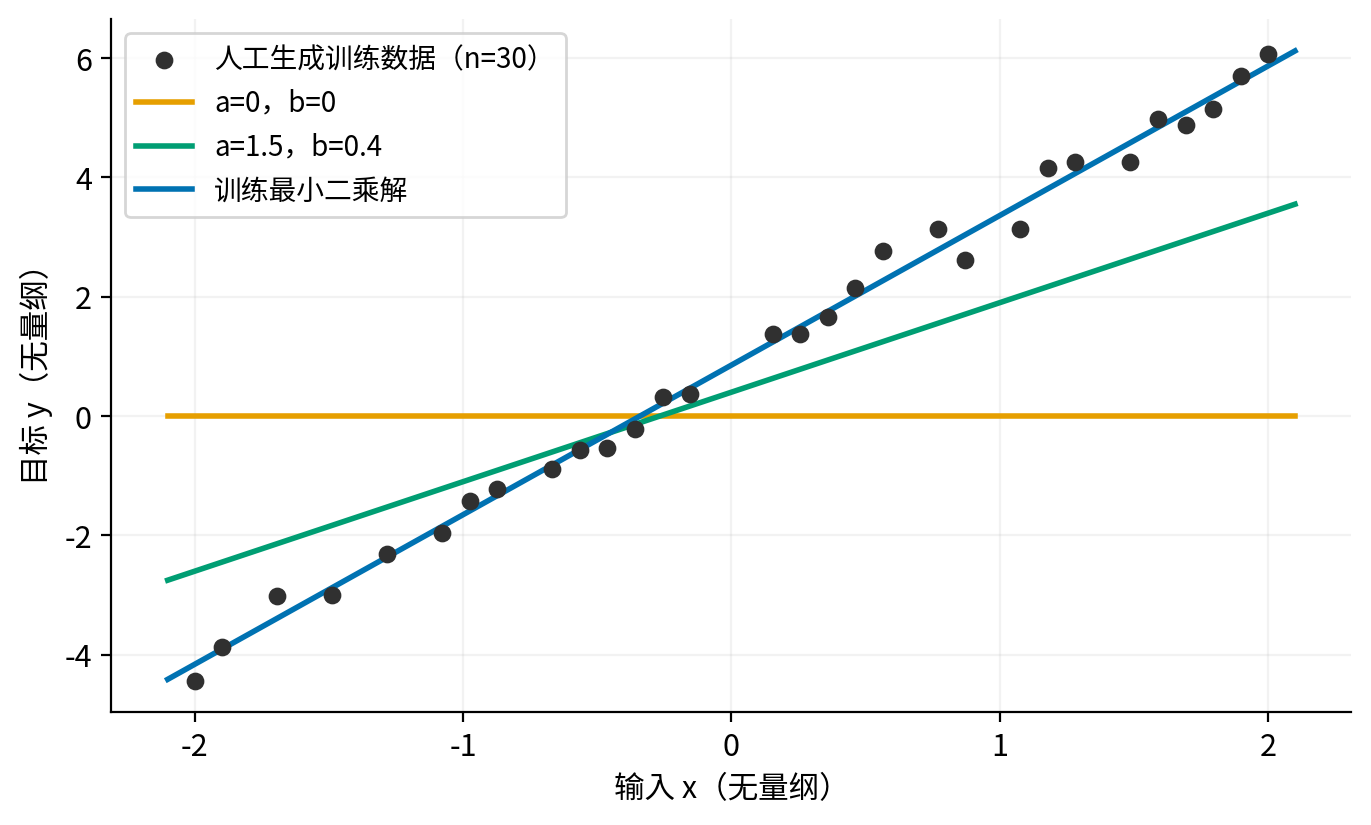
\includegraphics[width=0.92\linewidth]{figures/ch03_figure_1.png}\caption{人工生成数据中固定的30条训练记录，输入与目标均无量纲。三条直线属于相同模型形式。图中的训练最小二乘解仅作为后续求解的参照，未使用其余10条保留记录。}\end{figure}

\subsection{模型、目标和优化方法各回答什么}

在讨论一个学习算法时，最好把三个问题分别说清楚。模型表达回答``怎样从输入得到预测''；训练目标回答``怎样衡量当前参数是否合适''；优化方法回答``怎样寻找使目标较小的参数''。表3-1把本章的选择放在一起，后续章节会逐步替换其中的内容。

表3-1 本章训练问题的三个组成部分

\begin{longtable}[]{@{}
  >{\raggedright\arraybackslash}p{(\columnwidth - 4\tabcolsep) * \real{0.1441}}
  >{\raggedright\arraybackslash}p{(\columnwidth - 4\tabcolsep) * \real{0.3314}}
  >{\raggedright\arraybackslash}p{(\columnwidth - 4\tabcolsep) * \real{0.5245}}@{}}
\toprule\noalign{}
\begin{minipage}[b]{\linewidth}\raggedright
\textbf{组成部分}
\end{minipage} & \begin{minipage}[b]{\linewidth}\raggedright
\textbf{本章的具体选择}
\end{minipage} & \begin{minipage}[b]{\linewidth}\raggedright
\textbf{它规定的事情}
\end{minipage} \\
\midrule\noalign{}
\endhead
\bottomrule\noalign{}
\endlastfoot
模型表达 & \(\widehat{y} = ax + b\) & 给定输入与参数后怎样预测 \\
训练目标 & 训练数据上的半均方误差 & 怎样比较不同参数的拟合程度 \\
优化方法 & 梯度下降 & 怎样依据当前参数计算下一步参数 \\
\end{longtable}

同一个模型可以有不同的求解方法；同一种优化方法也能用于不同模型。梯度下降属于优化方法，不能与逻辑回归、决策树等预测模型放在同一层级上理解。sklearn 的官方说明也特别区分了随机梯度下降与由它训练的模型。{[}1{]} 到第5章，我们会比较线性回归的求解路径；到第6章，模型输出将与类别概率联系起来，但``模型---目标---求解''的区分仍然成立。

\subsection{模型形式、目标函数与求解方法是三个选择}
对同一批直线数据，可以保持模型$\hat y=ax+b$不变，分别最小化平方误差和绝对误差；也可以保持平方误差目标不变，分别采用直接最小二乘求解和梯度下降。前一种比较改变了“什么参数算好”，后一种比较改变了“怎样找到这些参数”。若两者同时改变，结果差异就不能仅归因于优化器。

这个区分解释了为什么一个软件接口只有一行，背后却有多层选择。\texttt{fit}是统一的操作名称，输入包括数据和配置，输出是已拟合状态；它不承诺内部一定执行固定次数的梯度更新。近邻方法保存并组织训练记录，决策树比较候选划分，普通最小二乘可以用矩阵分解。后面每章都需要分别回答模型、目标与学习过程这三个问题。

\section{从预测误差到损失函数}

\subsection{为什么不能直接平均正负误差}

给定一个预测，最直接的误差是预测与目标之差。本章采用统一约定：

\[e_{i} = {\widehat{y}}_{i} - y_{i}.\]

\(e_{i}\) 称为第 \(i\) 条记录的残差。它为正，表示预测偏高；为负，表示预测偏低。也有书籍采用相反的残差符号，只要在损失和求导中保持一致即可。这里明确符号，是为了让后面的更新方向可以逐项核对。

考虑表3-2中的三个点。它们是专为手算构造的无噪声例子，与后面的40条CSV记录相互独立。真实关系在此被直接设定为 \(y = 2x + 1\)，当前模型却取 \(a = 1,b = 1\)。

表3-2 用于手算的人工三点例子

\begin{longtable}[]{@{}
  >{\raggedright\arraybackslash}p{(\columnwidth - 8\tabcolsep) * \real{0.1657}}
  >{\raggedright\arraybackslash}p{(\columnwidth - 8\tabcolsep) * \real{0.1657}}
  >{\raggedright\arraybackslash}p{(\columnwidth - 8\tabcolsep) * \real{0.2377}}
  >{\raggedright\arraybackslash}p{(\columnwidth - 8\tabcolsep) * \real{0.1945}}
  >{\raggedright\arraybackslash}p{(\columnwidth - 8\tabcolsep) * \real{0.2363}}@{}}
\toprule\noalign{}
\begin{minipage}[b]{\linewidth}\raggedright
\textbf{输入} \(x_{i}\)
\end{minipage} & \begin{minipage}[b]{\linewidth}\raggedright
\textbf{目标} \(y_{i}\)
\end{minipage} & \begin{minipage}[b]{\linewidth}\raggedright
\textbf{当前预测} \({\widehat{y}}_{i}\)
\end{minipage} & \begin{minipage}[b]{\linewidth}\raggedright
\textbf{残差} \(e_{i}\)
\end{minipage} & \begin{minipage}[b]{\linewidth}\raggedright
\textbf{残差平方} \(e_{i}^{2}\)
\end{minipage} \\
\midrule\noalign{}
\endhead
\bottomrule\noalign{}
\endlastfoot
\(- 1\) & \(- 1\) & \(0\) & \(1\) & \(1\) \\
\(0\) & \(1\) & \(1\) & \(0\) & \(0\) \\
\(1\) & \(3\) & \(2\) & \(- 1\) & \(1\) \\
\end{longtable}

三条残差的平均值是0，但其中两条预测并不正确。这说明平均带符号误差可以反映整体偏高或偏低，却不能独自衡量预测偏离的大小。正负误差可能相互抵消。若把每个残差先平方再平均，偏高和偏低都会产生非负的代价，抵消就不会发生。

本章把单条记录的损失定义为：

\[\ell_{i} = \frac{1}{2}\left( {\widehat{y}}_{i} - y_{i} \right)^{2} = \frac{1}{2}e_{i}^{2}.\]

这里的 \(\ell_{i}\) 是该记录的\textbf{平方损失}，系数 \(1/2\) 是为了使后面的导数更简洁。对 \(n\) 条训练记录取平均，得到：

\[J(a,b) = \frac{1}{n}\sum_{i = 1}^{n}\ell_{i} = \frac{1}{2n}\sum_{i = 1}^{n}\left( ax_{i} + b - y_{i} \right)^{2}.\]

\(J\) 是当前参数在整批训练记录上的\textbf{半均方误差}。表3-2中，\(J = (1 + 0 + 1)/(2 \times 3) = 1/3\)。通常所说的均方误差，即 MSE，没有前面的 \(1/2\)，因此本例 MSE 为 \(2/3\)。本章所有标为``训练损失''的直线实验都采用半均方误差，不能把图中的数值直接当作未经换算的 MSE。

\subsection{损失函数表达了怎样的偏好}

平方并不只是消除了符号。它还使较大的残差受到较重的惩罚：残差的绝对值加倍，平方项变为原来的四倍。因此，少数偏离较远的记录可能明显影响最终直线。面对实验数据中的异常读数时，这种性质既可能帮助模型认真处理大偏差，也可能使错误记录牵动拟合结果。选择损失函数，就是规定模型怎样看待不同类型的预测错误。

平方损失不是唯一选择。绝对损失使用残差绝对值，其他损失可以在小残差和大残差区域采用不同惩罚。分类任务的输出和目标含义不同，也需要适合该任务的目标函数。第6章讨论逻辑回归时，我们会从概率预测引出相应损失，而不会直接把类别编号当作普通连续测量值来套用本章例子。这里先把一种损失理解透彻，比提前记住许多名称更有用。

损失的量纲和数值大小也要结合目标理解。如果 \(y\) 表示某个带单位的测量量，平方损失就带有该单位的平方。把目标由一种单位换成另一种单位，即使预测关系在物理上没有改变，损失数字也会变化。因此，不同任务的损失大小通常不能直接横向比较。在科学数据中，各条记录还可能有不同的测量不确定性，是否应赋予不同权重，需要结合误差模型另行判断。本章的等权平均只对应所有训练记录采用相同权重的教学设定。

\subsection{训练损失与评价指标的联系}

训练损失直接参与参数寻找；评价指标用于回答模型表现的问题。二者可以使用相同的数学形式，但使用的数据和承担的任务仍需区分。例如，MSE既可以与回归训练目标有关，也可以在未参与训练的数据上计算，作为评价结果。反过来，有些便于解释的评价指标并不适合直接用于梯度更新。

本章反复绘制的曲线使用的都是训练记录。它们告诉我们优化过程有没有改善当前训练目标，不能独自说明模型能否预测新对象。一个算法把训练损失降得很低，可能是学到了稳定关系，也可能过度适应了当前样本；这需要额外证据区分。先把``当前数据上拟合得怎样''与``新数据上表现怎样''分开，后续的验证、测试和泛化概念就更容易理解。

\section{经验损失 正则化与训练目标}

\subsection{从有限样本出发的目标}

我们希望模型在未来遇到的样本上也有较小误差，但未来所有可能的样本并没有同时摆在面前。训练时能够直接计算的，是已有训练样本上的平均损失。因此，上一节的 \(J\) 也称为\textbf{经验损失}。``经验''指它来自有限数据，并不表示它只是凭经验随意规定的数值。损失的形式由建模者选择，损失的具体数值则由数据和当前参数共同决定。

一旦训练数据和模型形式固定，每一组参数都有一个对应的经验损失。训练就是在参数空间中寻找较小的目标值。对于一条直线，参数空间有两个方向：一个方向改变斜率，另一个方向改变截距。不能因为数据散点画在 \(x\)、\(y\) 平面里，就把寻找参数想象成移动某条数据记录；优化所移动的是参数空间中的位置。

为什么不总是追求把训练损失降到零？首先，模型形式可能无法穿过所有点。其次，数据中的随机噪声不一定具有可预测性。更复杂的模型虽然可能把每条训练记录都贴得很近，却未必更适合后续样本。要理解这种取舍，除了选择模型形式，还需要认识另一种控制方式：正则化。

\subsection{在拟合误差之外增加约束偏好}

在本章的直线例子中，可在经验损失上增加一个与斜率大小有关的项：

\[J_{\lambda}(a,b) = J(a,b) + \frac{\lambda}{2}a^{2},\quad\quad\lambda \geq 0.\]

\(J_{\lambda}\) 表示加入正则化后的训练目标，\(\lambda\) 是控制惩罚强弱的非负数。这里使用平方型惩罚，是 L2 正则化的一个简单例子；为了突出斜率的作用，本例不惩罚截距。不同模型和软件对截距的处理可能不同，不能把这一约定当作全部方法的统一规则。本章的 \(\lambda\) 专指上述``半均方误差加 \(\lambda a^{2}/2\)''的定义，不直接等同于所有 sklearn 估计器中的同名或类似选项；第5章会结合具体目标解释 Ridge 的 \texttt{alpha}。

当 \(\lambda = 0\) 时，目标只包含经验损失；当 \(\lambda > 0\) 时，算法除了希望拟合误差小，还要付出斜率过大的代价。参数调整需要平衡这两部分，而不是先把直线拟合好，再随意把斜率改小。正则化改变的是训练要解决的问题，所以通常也会改变最终参数。

利用本章30条人工训练记录，直接求解上述二次目标，可得到表3-3。这里的计算用于认识训练目标，不涉及保留数据上的表现。表中的数值按实际运行结果取六位小数。

表3-3 不同正则化强度对应的训练解，原始输入坐标，截距不惩罚

\begin{longtable}[]{@{}
  >{\raggedright\arraybackslash}p{(\columnwidth - 8\tabcolsep) * \real{0.1081}}
  >{\raggedright\arraybackslash}p{(\columnwidth - 8\tabcolsep) * \real{0.1801}}
  >{\raggedright\arraybackslash}p{(\columnwidth - 8\tabcolsep) * \real{0.1801}}
  >{\raggedright\arraybackslash}p{(\columnwidth - 8\tabcolsep) * \real{0.2305}}
  >{\raggedright\arraybackslash}p{(\columnwidth - 8\tabcolsep) * \real{0.3012}}@{}}
\toprule\noalign{}
\begin{minipage}[b]{\linewidth}\raggedright
\(\lambda\)
\end{minipage} & \begin{minipage}[b]{\linewidth}\raggedright
\textbf{斜率} \(a\)
\end{minipage} & \begin{minipage}[b]{\linewidth}\raggedright
\textbf{截距} \(b\)
\end{minipage} & \begin{minipage}[b]{\linewidth}\raggedright
\textbf{经验损失} \(J\)
\end{minipage} & \begin{minipage}[b]{\linewidth}\raggedright
\textbf{正则化项} \(\lambda a^{2}/2\)
\end{minipage} \\
\midrule\noalign{}
\endhead
\bottomrule\noalign{}
\endlastfoot
0 & 2.506900 & 0.853364 & 0.026641 & 0.000000 \\
0.1 & 2.342148 & 0.873641 & 0.045935 & 0.274283 \\
1.0 & 1.471686 & 0.980775 & 0.788396 & 1.082930 \\
\end{longtable}

随着惩罚增强，斜率向0收缩，经验损失却变大了。这并不说明优化失败：算法优化的是包含惩罚项的整个目标。不同 \(\lambda\) 对应不同目标函数，也不能把它们各自的目标最小值直接排在一起，选数值最小者作为最佳正则化强度。应当怎样选择强度、怎样检验它是否改善新样本上的表现，是第4章和第5章要进一步解决的问题。

正则化是一种建模偏好，不能替代科学知识。对于本例，它鼓励较小的斜率，却没有自动判断哪个斜率符合某条物理定律。斜率的数字还依赖输入单位；改用不同尺度的输入，同一预测关系可能对应很不一样的参数大小。因此，特征处理、正则化形式和强度需要一起理解。第3.8节的尺度实验先考察没有正则化时的优化过程，以免同时改变太多因素。

\subsection{训练目标清楚之后，仍需选择求解方法}

写出目标函数，并不意味着只能通过梯度下降求解。对于结构简单的最小二乘问题，可以利用专门的数值线性代数方法；对于其他问题，可能使用不同的迭代优化或结构搜索。本章训练直线时亲手写出梯度下降，是为了把参数更新过程展开来看。

在 sklearn 中，\texttt{fit} 是统一接口名称，表示估计器根据数据完成拟合，它不保证内部使用某一种优化方法。本章传入普通稠密数据、保持默认非负约束设置时，\texttt{LinearRegression} 使用最小二乘数值求解，并不默认执行后面所写的梯度下降循环。{[}2{]} 所以，仅凭代码出现了 \texttt{model.fit(X,\ y)}，无法判断它怎样学习；需要结合模型与求解器的说明。

这一点也关系到后续神经网络学习。梯度下降利用梯度更新参数；反向传播则是对神经网络这类复合计算高效计算梯度的方法。两者承担不同工作。第12章会在本章的更新规则之上解释梯度怎样逐层得到，这里先集中理解``给定梯度后怎样改变参数''。

\section{导数 梯度与参数变化}

\subsection{导数告诉我们局部变化方向}

先只考虑一个可调整参数 \(w\)，把目标写成 \(J(w)\)。导数 \(J'(w)\) 描述：在当前位置附近，参数发生很小变化时，目标大致怎样变化。若 \(J'(w) > 0\)，在足够小的范围内增大 \(w\) 会使目标增大，因此可以尝试减小 \(w\)；若 \(J'(w) < 0\)，则可以尝试增大 \(w\)。这里反复强调``附近''和``足够小''，因为导数是局部信息，并不保证任意大的一步都有效。

用一个小改变量 \(\Delta w\) 表示参数的移动，可以把这个关系简写为：

\[J(w + \Delta w) \approx J(w) + J'(w)\Delta w.\]

式中，\(\Delta w\) 越小，局部线性近似通常越有用。要让右侧的变化项为负，可以让 \(\Delta w\) 与导数符号相反。这就是沿负导数方向更新的直觉来源。但近似式没有告诉我们具体该走多远；步长还需由下一节的学习率控制。

本章用以下人为规定的函数作示意：

\[J(w) = \frac{1}{2}(w - 3)^{2},\quad\quad J'(w) = w - 3.\]

这里的 \(w\) 只是示意参数，\(J\) 也不是由CSV数据计算得到的损失。我们特意把最小点设在 \(w = 3\)，以便直接核对更新方向。若 \(w = 0\)，导数为 \(- 3\)，应尝试增大参数；若 \(w = 4\)，导数为1，应尝试减小参数。越靠近3，导数的绝对值越小。在这个简单例子中，梯度也自然提供了``接近谷底时减小移动幅度''的信息。

\subsection{多个参数需要一个方向向量}

直线模型有两个参数，只知道改变斜率的影响还不够。我们分别考察保持 \(b\) 不变而改变 \(a\)，以及保持 \(a\) 不变而改变 \(b\) 时，目标怎样变化。这两个变化率称为偏导数。把它们组成向量，就得到\textbf{梯度}：

\[\nabla J(a,b) = \begin{pmatrix}
\frac{\partial J}{\partial a} \\
\frac{\partial J}{\partial b}
\end{pmatrix}.\]

\(\nabla\) 是表示梯度的符号。它的两个分量分别对应斜率方向和截距方向，顺序必须与参数向量 \((a,b)^{\mathsf{T}}\) 一致。在当前参数坐标采用通常的欧氏距离时，梯度指向局部增大目标最快的方向，负梯度则给出相反方向。改变参数的数值尺度，会改变这种几何关系，这也是标准化可能影响优化的重要原因。

对本章的半均方误差，只需保留下面两条实用公式：

\[\frac{\partial J}{\partial a} = \frac{1}{n}\sum_{i = 1}^{n}e_{i}x_{i},\quad\quad\frac{\partial J}{\partial b} = \frac{1}{n}\sum_{i = 1}^{n}e_{i}.\]

其中，\(e_{i} = ax_{i} + b - y_{i}\) 是当前参数产生的残差。截距每增加一点，会同样改变所有预测，因此它的梯度是平均残差；斜率的改变对不同输入的影响不同，所以它的梯度还包含 \(x_{i}\)。理解这两个分量的来源，比只记住公式更能帮助我们检查代码。

回到表3-2。当前残差为1、0、\(- 1\)，输入为\(- 1\)、0、1。因此，斜率方向的梯度为\(( - 1 + 0 - 1)/3 = - 2/3\)，截距方向的梯度为0。模型没有整体向上或向下平移的需要，但斜率偏小，需要增大。这也解释了为什么``平均残差为0''并不表示已经找到最优直线：它只能使这里的截距梯度为0，斜率梯度仍然不为0。

\subsection{怎样理解梯度接近零}

若所有梯度分量都接近零，沿很小的参数变化已经难以获得明显的一阶下降。对于本章这种输入并不全相同的直线最小二乘问题，损失面呈碗形，存在唯一最小点，因此小梯度是接近最优解的重要信号。对于复杂模型，目标面可能出现不同结构，梯度为零也可能对应其他驻点，不能不加条件地解释为找到了全局最优模型。

在实际计算中，还要留意梯度与数据处理的联系。若输入中有极大的数值，斜率梯度中的 \(e_{i}x_{i}\) 也可能很大；若数据里有异常目标，残差本身可能主导更新。梯度不是脱离数据的抽象箭头，它把当前模型、目标定义和样本数值联系起来。观察梯度异常时，应当同时检查这些来源，而不是只反复增加迭代次数。

\subsection{用数值差分检查解析梯度}
复杂模型的梯度公式可能写错。一个不依赖同一推导的检查办法，是直接轻微改变参数，观察目标变化。对第$j$个参数，中心差分近似为
\[
\frac{\partial J}{\partial\theta_j}\approx
\frac{J(\boldsymbol\theta+\varepsilon\mathbf e_j)-J(\boldsymbol\theta-\varepsilon\mathbf e_j)}{2\varepsilon},
\]
其中$\mathbf e_j$只在第$j$个位置为1。这个方法需要两次目标计算，而不是调用已写好的梯度函数，因此能够发现许多符号、系数和求和方向错误。$\varepsilon$太大时截断误差明显，太小时浮点减法可能丢失有效数字；教学中可用$10^{-4},10^{-5},10^{-6}$检查结果是否稳定。

新增检查采用三点$x=(1,2,3)$、$y=(3,5,8)$，初始斜率1、截距0，目标为\emph{MSE}而非本章基础实验的半MSE。解析梯度为$(-46/3,-20/3)$，中心差分与之吻合。这里专门改用MSE，是为了再次核对目标定义：乘在目标前的常数会改变梯度，却不改变无正则情况下的最小点。代码与公式必须使用同一个约定。

数值差分检查通过不代表整个模型正确。它主要说明当前位置附近的目标函数和梯度实现相容，仍需检查数据、目标定义及评价过程。对于分段不可导点，应避开拐点或明确采用的导数约定，第12章将在ReLU网络上再次使用这一检查。

\section{梯度下降 学习率与停止条件}

\subsection{从方向得到一次更新}

有了梯度，还需要决定每次沿该方向移动多少。令 \(\eta > 0\) 表示\textbf{学习率}，\(t\) 表示已经完成的更新次数，梯度下降写成：

\[\mathbf{\theta}^{(t + 1)} = \mathbf{\theta}^{(t)} - \eta\nabla J\left( \mathbf{\theta}^{(t)} \right).\]

\(\mathbf{\theta}^{(t)}\) 是第 \(t\) 步参数，右侧梯度也必须在这一组旧参数上计算。对直线来说，应先算出两个梯度分量，再同时更新 \(a\) 和 \(b\)。若先改变 \(a\)，再用新 \(a\) 计算 \(b\) 的梯度，就已经改变了这里定义的更新规则。

表3-2的例子可立即用于一次检查。取学习率 \(\eta = 0.3\)，从 \(a = 1,b = 1\) 出发，由于梯度为 \(( - 2/3,0)^{\mathsf{T}}\)，更新后得到 \(a = 1.2,b = 1\)。新的残差为0.8、0、\(- 0.8\)，半均方误差从 \(1/3\) 降为 \(0.64/3 \approx 0.213333\)。这个短计算把方向、步长、预测和损失连成了一条完整链条。

再看单参数示意函数。从 \(w^{(0)} = 0\) 出发，取 \(\eta = 0.5\)，有：

\[\begin{matrix}
w^{(1)} & = 0 - 0.5 \times (0 - 3) = 1.5, \\
w^{(2)} & = 1.5 - 0.5 \times (1.5 - 3) = 2.25.
\end{matrix}\]

两步之后，损失依次由4.5降到1.125，再降到0.28125。参数逐渐接近3，梯度的绝对值也随之减小。这里没有使用``知道答案以后直接把参数设成3''的做法，程序每一步只依据当前位置的导数行动。

\subsection{学习率过小、合适和过大}

图3-2比较了四个学习率，初始位置和示意目标完全相同。学习率0.1的参数一直从左侧接近最小点，但12步后仍只有约2.152711。学习率0.5接近得更快，12步后约为2.999268。学习率1.5每一步都会跨过最小点，参数在两侧交替，不过偏离幅度越来越小。学习率2.1也左右交替，却越走越远，12步后的损失约44.323797，高于起点的4.5。

\begin{figure}[htbp]\centering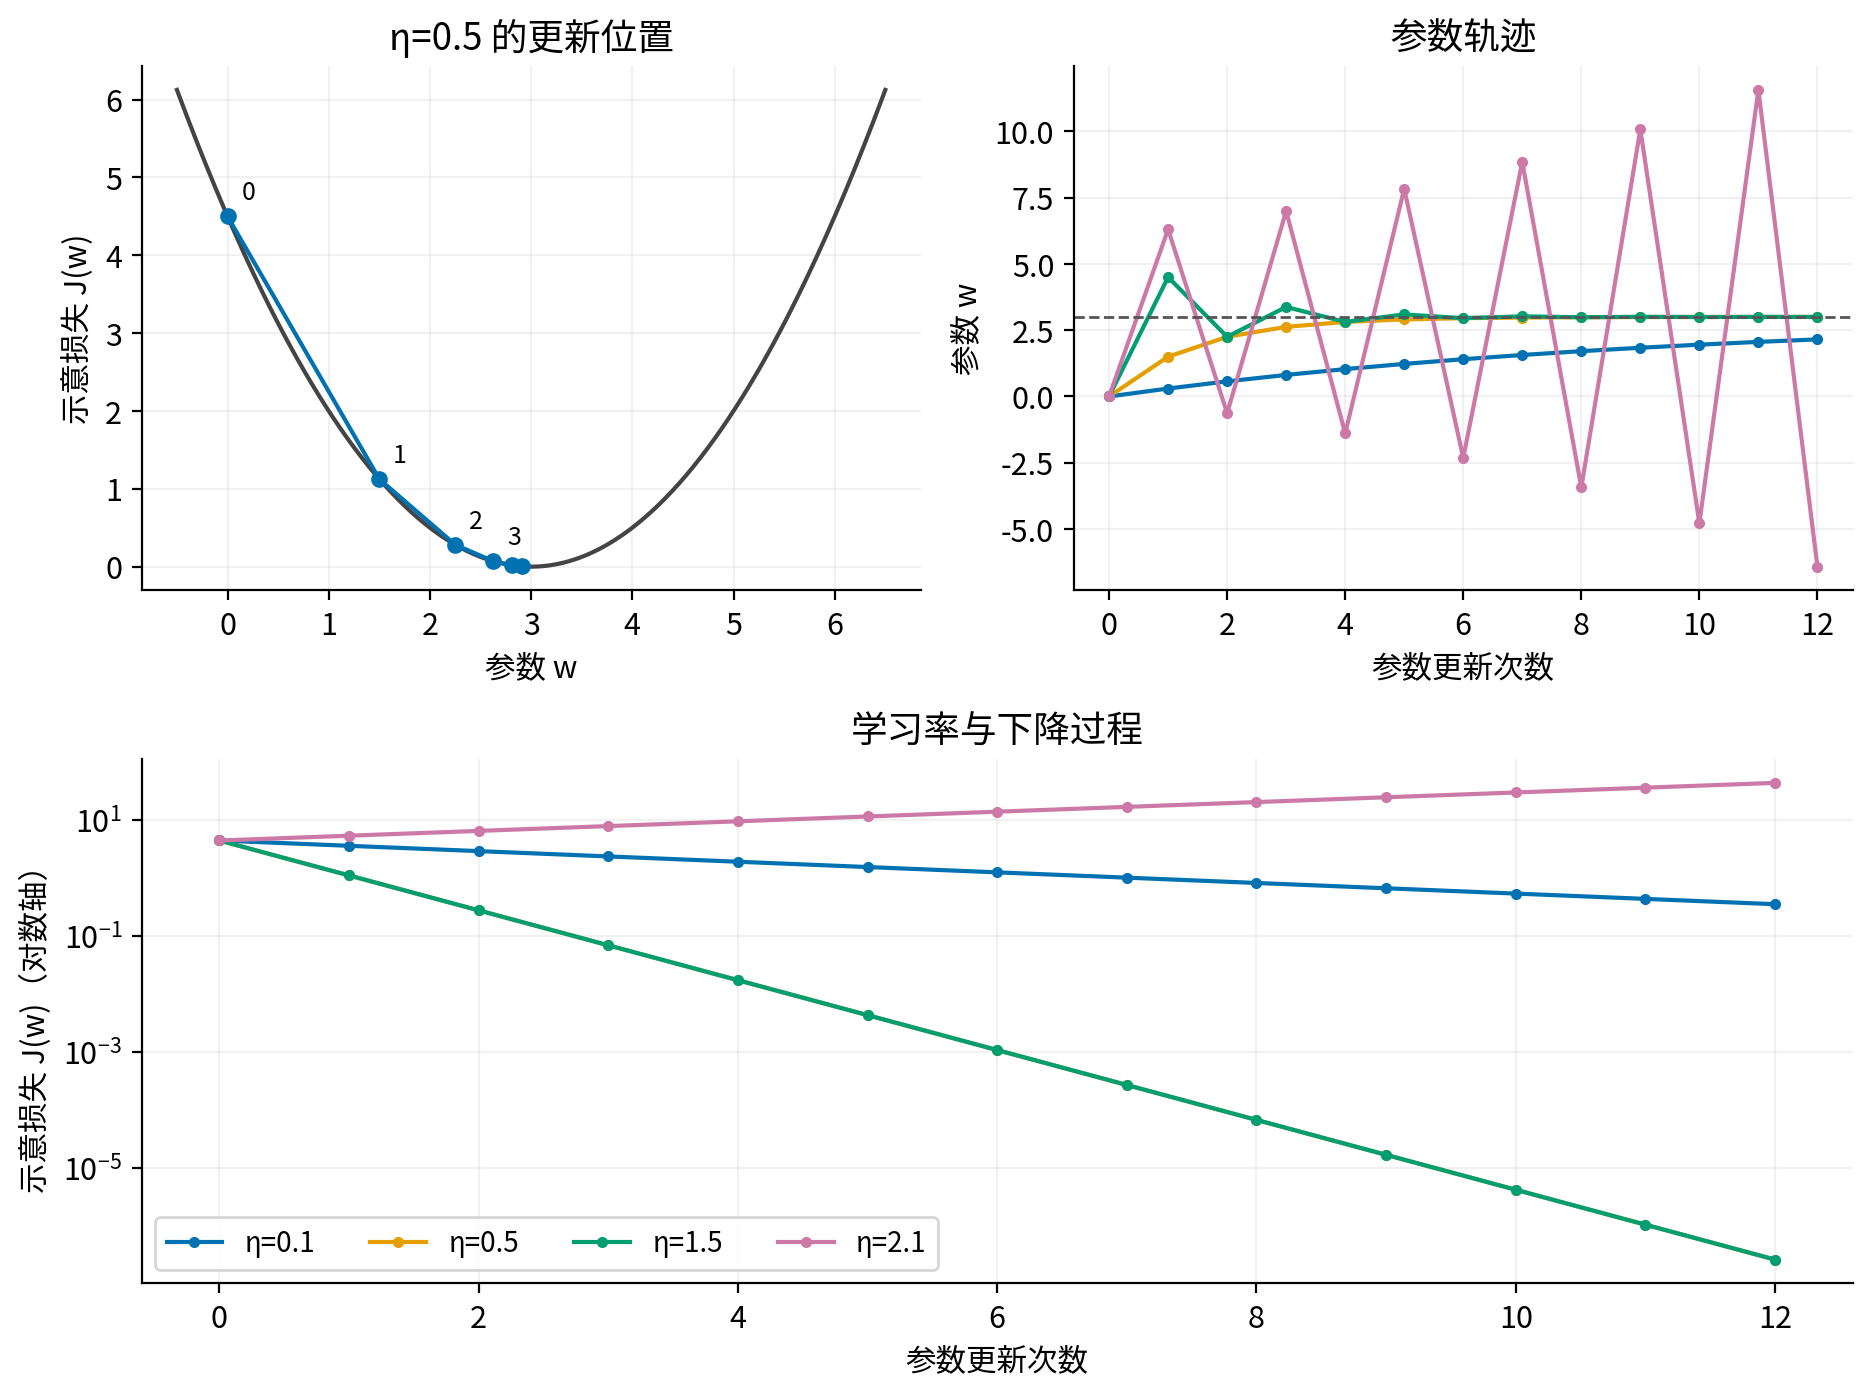
\includegraphics[width=0.92\linewidth]{figures/ch03_figure_2.png}\caption{人为设定的示意损失 \(J(w) = (w - 3)^{2}/2\)，不使用任何观测或训练记录。上左图标出学习率0.5的前几步位置，其横轴为参数 \(w\)；上右图显示参数轨迹，下图显示损失轨迹，两者横轴均为参数更新次数。下图采用对数纵轴；学习率0.5与1.5的损失曲线完全重合。}\end{figure}

这个例子说明，出现振荡不一定意味着发散。应当看振荡幅度是缩小、保持还是放大，也要观察损失怎样变化。对于本例，把更新式整理一下，可以得到：

\[w^{(t + 1)} - 3 = (1 - \eta)\left( w^{(t)} - 3 \right).\]

因此，学习率0.5和1.5虽然轨迹不同，偏离最小点的绝对值每一步都减半，损失曲线恰好重合。学习率2.0会使参数在0和6之间来回，损失保持4.5。这个边界取决于当前示意函数的形状，不能据此说``所有任务的学习率小于2就安全''。换一个目标、换一种特征尺度，适合的学习率都可能改变。

同样需要注意目标前面的常数。如果把半均方误差改成MSE，最小点不变，梯度却整体扩大一倍。在没有同步调整学习率时，更新轨迹就会改变。这是比较不同教材、软件或代码时经常遇到的细节：数值上相同的学习率，只有在目标定义和更新规则也一致时才具有相同意义。

\subsection{何时停止，以及停止意味着什么}

最直观的停止方式是规定最大更新次数。它容易实现，可以限制计算量，但``用完了次数''只说明程序执行结束，不说明一定接近最小点。另一种方式是观察相邻若干步的目标变化是否很小，或梯度范数是否小于设定阈值。梯度范数是把多个梯度分量合起来衡量其大小的量。设置这些阈值时，要考虑目标和参数的尺度，不能把某个小数机械地复制到所有问题。

损失变平也需要解释。如果学习率极小，参数几乎没有移动，曲线可能很平，却仍离最优值很远；若计算达到浮点精度所能分辨的范围，继续迭代也可能没有可见改善。因此，判断训练状态时，最好同时查看目标、参数变化和必要的参照值，而不是只看图是否平滑。

本章直线基础实验固定执行120次更新，方便不同学生复现同一轨迹。这个次数是教学中的停止设置，程序并没有利用保留数据决定何时停止。尺度实验另设损失超过 \(10^{12}\) 时的保护停止，以防明显发散继续造成数值问题；这种停止代表需要检查学习率或输入尺度，绝不表示成功收敛。第4章会进一步说明利用验证数据观察泛化表现的做法，它与这里仅检查训练优化状态的停止判断承担不同任务。

\subsection{选读：一个能精确分析的收敛条件}
对二次目标$J(\boldsymbol\theta)=\frac12(\boldsymbol\theta-\boldsymbol\theta^*)^{\mathsf T}H(\boldsymbol\theta-\boldsymbol\theta^*)+c$，假定$H$为对称正定矩阵。$H$称为Hessian矩阵，记录目标对参数的二阶变化，在本例中为常数。设误差$\mathbf e_t=\boldsymbol\theta_t-\boldsymbol\theta^*$，梯度更新成为
\[
\mathbf e_{t+1}=(I-\eta H)\mathbf e_t.
\]
沿$H$的一个特征向量方向，误差每步乘以$1-\eta\lambda_j$。要让各方向的误差都缩小，需要所有$|1-\eta\lambda_j|<1$，因此可用的恒定学习率满足
\[
0<\eta<\frac{2}{\lambda_{\max}(H)}.
\]
这一推导只用了对称矩阵特征分解，不要求证明一般非线性优化定理。它说明最陡方向限制了步长，而较平缓方向可能仍然走得很慢。不同方向曲率相差很大时，一个共同步长难以兼顾，这为特征缩放提供了定量解释。

在上节新增的三点MSE例子中，设计矩阵每行为$(x_i,1)$，$H=2D^{\mathsf T}D/3$，其最大特征值约11.09294，因此这一个二次问题的稳定上界约为0.180295。不能把这个数复制到其他数据，也不能把二次正定模型的结论无条件推广到所有神经网络。神经网络的局部曲率随参数变化，非凸问题还存在不同驻点。

这一分析也澄清“负梯度是最快下降方向”的条件：它是当前点的一阶局部描述，并以欧氏长度约束步长方向。走有限的一大步仍可能越过低处。方向选择、步长选择与全局是否收敛是相关但不同的问题。

\section{批量 随机与小批量更新}

\subsection{每次梯度可以用多少条记录}

前面的直线梯度由全部 \(n\) 条训练记录的平均贡献计算得到。每更新一次，都遍历全部训练记录，这叫\textbf{全批量梯度下降}，也常简称批量梯度下降。它使我们看到当前训练目标的完整梯度；在本章的二次目标上配合足够小的学习率，可以得到平稳的下降过程。当样本很多时，每次更新前都处理全部记录的计算开销也会增大。

另一种办法是每次只使用一条记录的损失梯度进行更新，称为\textbf{随机梯度下降}，英文缩写为 SGD。实践中可以随机抽取记录，也可以在每轮开始时打乱顺序，再依次使用每条记录。本章采用后一种方式。它让参数在读完全部记录之前就多次变化，但单条记录的方向未必与完整训练梯度相同。

在两者之间，可以把记录分成若干较小的批次，每次用一批记录的平均梯度更新，这就是\textbf{小批量梯度下降}。设当前批次的索引集合为 \(B\)，批次大小为 \(m = |B|\)，则直线模型的两个梯度分量改写为：

\[g_{a} = \frac{1}{m}\sum_{i \in B}^{}e_{i}x_{i},\quad\quad g_{b} = \frac{1}{m}\sum_{i \in B}^{}e_{i}.\]

这里的残差都由当前参数计算。批次大小等于 \(n\) 时退回全批量，等于1时成为单样本更新。若最后一批不足预设大小，应按实际包含的记录数取平均。不能一边改变批次大小，一边仍除以固定的训练样本总数，否则也改变了梯度的数值尺度。

\subsection{一次更新与一轮遍历不同}

\textbf{一次迭代}在本章中专指一次参数更新；\textbf{一轮}，即 epoch，表示训练记录完整参与一次遍历。以30条训练记录为例，全批量每轮只更新1次，批量大小为6时每轮更新5次，单样本更新每轮则更新30次。因此，规定``训练80轮''与规定``更新80次''完全不同。

表3-4给出本章批量实验的计数。三种方式采用相同的初始参数、相同的常数学习率0.1和同一份训练标准化数据，均遍历80轮。这样，每种方式都有2400次样本参与更新，但更新次数不同。图中记录完整训练损失所增加的计算不计入样本访问量，因此这些数目也不能直接当作实际耗时。

表3-4 三种批量方式的计算安排

\begin{longtable}[]{@{}
  >{\raggedright\arraybackslash}p{(\columnwidth - 8\tabcolsep) * \real{0.1441}}
  >{\raggedright\arraybackslash}p{(\columnwidth - 8\tabcolsep) * \real{0.2089}}
  >{\raggedright\arraybackslash}p{(\columnwidth - 8\tabcolsep) * \real{0.1945}}
  >{\raggedright\arraybackslash}p{(\columnwidth - 8\tabcolsep) * \real{0.2017}}
  >{\raggedright\arraybackslash}p{(\columnwidth - 8\tabcolsep) * \real{0.2508}}@{}}
\toprule\noalign{}
\begin{minipage}[b]{\linewidth}\raggedright
\textbf{方式}
\end{minipage} & \begin{minipage}[b]{\linewidth}\raggedright
\textbf{每次更新使用记录数}
\end{minipage} & \begin{minipage}[b]{\linewidth}\raggedright
\textbf{每轮更新次数}
\end{minipage} & \begin{minipage}[b]{\linewidth}\raggedright
\textbf{80轮更新次数}
\end{minipage} & \begin{minipage}[b]{\linewidth}\raggedright
\textbf{参与更新的样本总次数}
\end{minipage} \\
\midrule\noalign{}
\endhead
\bottomrule\noalign{}
\endlastfoot
全批量 & 30 & 1 & 80 & 2400 \\
小批量 & 6 & 5 & 400 & 2400 \\
随机 & 1 & 30 & 2400 & 2400 \\
\end{longtable}

这一比较控制了数据遍历量，却没有使三种方法的全部条件都等价。例如，它们更新参数的频率不同，适合的学习率设置也未必相同。设计对照实验时，应该先说明要控制什么，再解释结果。本章用这些条件呈现不同更新方式的特点，不把一个小数据实验当作一般性的速度排名。

\subsection{为什么损失曲线会有波动}

在第3.8节的图3-5中，我们在每次更新后都用全部30条训练记录计算半均方误差。这样，三条曲线的纵坐标具有同一含义。小批量或单样本梯度可能使当前批次的拟合改善，却让其他记录的拟合稍差，所以完整训练损失不保证每一步都下降。观察到某一步上升，不能立即认定程序有误；应结合上升幅度、长期趋势和更新方式判断。

当参数已经接近最小点时，这种区别更加明显。全批量梯度接近零，并不意味着每一条记录的梯度都接近零。含噪声的数据通常不可能被同一条直线全部穿过，单条记录仍会把参数拉向不同方向。使用不变的学习率时，随机更新因而可能在最小点附近持续波动。减小后期学习率或使用其他策略可以改变这种现象，但也会引入新的设置，本章教师Notebook保留一个递减学习率的选做例子。

本次固定打乱种子为42时，全批量、小批量和随机方式的末步训练半均方误差分别约为0.02664172、0.02664471和0.02734320。更换打乱种子为0至4，随机方式的末步结果在约0.02689578至0.02984611之间变化。在这组固定设置下，随机和小批量方式的末步参数会受到样本顺序影响；全批量方式在本程序中不打乱顺序，其结果不随该种子变化。不能据此宣布某种方法在所有任务中更好。

实践中，``SGD''有时也被宽泛地用于包含小批量的随机优化方法。阅读资料时要查看实际批量大小，而不是只看名称。sklearn 的 \texttt{SGDRegressor} 则是一个采用随机梯度学习线性模型的具体估计器，不能把其默认设置与本章手写循环直接视为相同。{[}1{]} 本章先明确每次用多少条记录、怎样取平均和怎样计步，后续再学习具体工具的参数就不容易混淆。

\subsection{随机梯度为什么可以估计完整梯度}
若每条训练记录等概率被抽取，单样本梯度的平均满足
\[
\mathbb E_i[\nabla\ell_i(\boldsymbol\theta)]
=\frac1n\sum_{i=1}^n\nabla\ell_i(\boldsymbol\theta)=\nabla J(\boldsymbol\theta)
\]
（这里$J$指数据平均损失）。于是随机梯度虽然一次可能朝向不同方向，在上述抽样条件和固定参数处，其期望等于完整梯度。对独立均匀抽取的小批量，批梯度平均具有同样性质。\textbf{被用来估计梯度的是梯度向量，不是标量损失值本身。}

实践中每轮打乱后无放回遍历，与每步独立有放回抽样并不完全相同。由于参数不断改变，也不能简单把一轮全部更新等同于在同一个参数点计算完整梯度。这个差别无需在入门时展开证明，但可以通过改变样本顺序观察不同轨迹。

重复同一个随机种子得到相同轨迹，是复现检查；改变随机种子考察末步参数与验证表现的波动，是稳定性检查。二者都需要做，但回答的问题不同。不能只汇报恰好收敛最快或误差最低的种子。

\section{模型参数与超参数}

\subsection{哪些量由拟合得到，哪些量由我们设置}

斜率 \(a\) 和截距 \(b\) 根据训练数据更新，是本章的模型参数。学习率、批量大小、最大更新次数和正则化强度则需要在一次训练开始前给出，或者按照预先规定的规则变化，通常称为\textbf{超参数}。表3-5列出两类量的区别。它们都影响结果，但进入学习流程的位置不同。

表3-5 本章常见数量的角色

\begin{longtable}[]{@{}
  >{\raggedright\arraybackslash}p{(\columnwidth - 4\tabcolsep) * \real{0.2738}}
  >{\raggedright\arraybackslash}p{(\columnwidth - 4\tabcolsep) * \real{0.2449}}
  >{\raggedright\arraybackslash}p{(\columnwidth - 4\tabcolsep) * \real{0.4813}}@{}}
\toprule\noalign{}
\begin{minipage}[b]{\linewidth}\raggedright
\textbf{数量}
\end{minipage} & \begin{minipage}[b]{\linewidth}\raggedright
\textbf{角色}
\end{minipage} & \begin{minipage}[b]{\linewidth}\raggedright
\textbf{在本章中的获得方式}
\end{minipage} \\
\midrule\noalign{}
\endhead
\bottomrule\noalign{}
\endlastfoot
斜率 \(a\)、截距 \(b\) & 模型参数 & 由训练记录与求解方法确定 \\
学习率 \(\eta\) & 优化超参数 & 在训练前设置或规定变化日程 \\
批量大小 & 优化超参数 & 规定每次更新使用多少条记录 \\
最大更新次数 & 训练停止设置 & 给定计算预算上限 \\
正则化强度 \(\lambda\) & 训练目标的超参数 & 控制误差与参数惩罚的权衡 \\
标准化均值与尺度 & 预处理的已学习状态 & 只由训练输入计算 \\
随机种子 & 复现设置 & 控制数据生成或打乱过程 \\
\end{longtable}

把某个量称为超参数，不意味着它不能通过数据辅助选择，而是说它不属于当前这一次拟合直接优化的那组模型参数。例如，可以比较几个学习率或正则化强度，但怎样比较、用哪些数据比较，需要一个独立于单次训练的选择流程。若反复查看本应保留的数据来选择设置，就破坏了其后续作为独立评价依据的作用。第4章会给出规范的模型选择流程，本章只观察训练机制，不利用保留记录调参。

有些设置改变学习的路径，有些设置改变学习的问题。学习率主要影响怎样寻找当前目标的较小值；正则化强度改变目标本身；选择直线或二次模型则改变可用的表达形式。如果把这些设置同时修改，即使最后损失不同，也很难说清原因。因此，初学阶段的对照实验应尽量一次改变一个明确因素，并记录其他条件。

\subsection{数据预处理也有从训练数据获得的状态}

标准化通常要先计算训练输入的均值和尺度，再把输入转成新的坐标。均值和尺度并不是模型的斜率、截距，但它们同样是从数据中得到的已学习状态。预测后续样本时，应沿用训练阶段得到的变换，不能每遇到一批新数据就自行重新定义坐标。

以 \texttt{StandardScaler} 为例，先在训练数据上 \texttt{fit}，再对需要处理的数据 \texttt{transform}。在尚未划分数据时就对全部记录拟合标准化器，会让保留部分参与流程的建立。sklearn 的实践文档明确要求先划分、再从训练部分学习预处理变换。{[}3{]} 本章已把40条人工记录固定划分为30条训练记录与10条保留记录，尺度实验的均值和尺度只来自训练记录。训练记录由固定随机索引确定，并不连续占据CSV的前30行，因此实际操作应以 \texttt{split\ ==\ \textquotesingle{}train\textquotesingle{}} 选行。保留记录虽然随数据包保存，仍不参与本章拟合、标准化或结果评价。

\subsection{阅读 sklearn 的参数名称}

软件接口中的 \texttt{parameter} 一词比本节的``模型参数''更宽。在 sklearn 中，构造估计器时传入的设置，以及 \texttt{get\_params()} 返回的内容，通常对应我们需要配置的选项；拟合后学到的系数则常保存为带结尾下划线的属性。例如，\texttt{LinearRegression} 拟合后的 \texttt{coef\_} 和 \texttt{intercept\_} 分别保存系数和截距。{[}2{]} 因此，不能因为接口把某个选项叫 parameter，就把它直接等同于通过损失最小化学到的权重。

具体计数方式也要查清。某个工具的 \texttt{max\_iter} 可能按数据遍历轮数计，另一个求解器则按内部迭代计，不能只看名称便假设它们完全一致。本章手写程序直接使用 \texttt{steps} 表示更新次数、\texttt{epochs} 表示遍历轮数，目的就是把这个差别显式表达出来。后续使用成熟估计器时，也应能从文档找到对应含义。

固定随机种子能够帮助复现给定环境中的一次运行，但它不能证明结果稳定。数据生成、数据划分和训练打乱也最好分别记录，避免只写一个含义不清的``随机种子''。当研究问题涉及随机波动时，还需要比较多个种子或多个合理划分。复现一次结果与证明结论稳健，是两项相互联系但并不相同的工作。

\section{一次可视化的模型训练实验}

\subsection{明确数据与本次实验的问题}

现在把前面的概念串成一次可重复的训练实验。我们要观察三个变化：参数从何处出发、拟合线如何移动、训练损失如何改变。基础实验保持模型形式和损失函数固定，再分别改变特征尺度及批量方式。运行之前先写下预测，运行之后用参数和曲线解释现象。

配套的 \texttt{line\_data.csv} 包含40条人工记录。输入在 \(\lbrack - 2,2\rbrack\) 上等间距取值，目标按下面的公式生成：

\[y_{i} = 2.5x_{i} + 0.8 + \varepsilon_{i},\quad\quad\varepsilon_{i} \sim \mathcal{N}\left( 0,{0.3}^{2} \right).\]

\(\varepsilon_{i}\) 是独立抽取的随机扰动，\(\mathcal{N}\left( 0,{0.3}^{2} \right)\) 表示均值为0、标准差为0.3的正态分布。这个噪声模型是为了构造可解释的小实验而设定的，不能当作所有物理或天文数据的通用误差模型。噪声生成种子为2026，划分种子为20261114，两者相互独立。固定划分中有30条训练记录，其余10条在本章保留不用。

文件包含 \texttt{sample\_id}、\texttt{x}、\texttt{y}、\texttt{split} 四列。身份字段与划分字段帮助追踪记录，但不作为模型输入。完整字段说明随数据提供。若把 \texttt{sample\_id} 编成数字送进模型，训练问题就与当前设计不同了；若把 \texttt{split} 当作特征，划分标记也会被错误地带入预测关系。

学生Notebook已经提供路径设置与依赖导入。读取并选择训练记录的关键代码为：

\begin{verbatim}
table = pd.read_csv(ROOT / "data" / "line_data.csv")
train = table.loc[table["split"].eq("train")].copy()
x = train["x"].to_numpy()
y = train["y"].to_numpy()
\end{verbatim}

Pandas表格用于识别列和筛选记录，NumPy数组用于计算。本例中 \texttt{x} 和 \texttt{y} 都是一维数组，各有30个元素。在调用 sklearn 估计器时，输入特征仍需保留二维结构，因此使用 \texttt{train{[}{[}"x"{]}{]}}；只有一个特征并不意味着样本维度可以省略。

\subsection{记录参数与训练损失}

初始参数设为 \(a = b = 0\)，学习率设为0.2，每一步使用全部30条训练记录。梯度函数直接对应第3.4节公式：

\begin{verbatim}
def gradient(x, y, theta):
    error = theta[0] * x + theta[1] - y
    return np.array([
        np.mean(error * x),
        np.mean(error)
    ])
\end{verbatim}

其中 \texttt{theta{[}0{]}} 保存斜率，\texttt{theta{[}1{]}} 保存截距。更新时只需写 \texttt{theta\ =\ theta\ -\ lr\ *\ gradient(x,\ y,\ theta)}。完整Notebook在更新前后保存参数和训练损失，且把初始化记录为第0步；这样，图中的第1步始终表示已经完成一次更新，不会与第一次打印记录混淆。

表3-6摘取了实际运行中的几个时刻。第1步之后，斜率和截距已朝正确方向移动；第5步时主要趋势已经出现；第20步后，剩余变化在图上很难分辨。第120步的半均方误差约为0.02664148，并没有降到零。

表3-6 全批量梯度下降的参数记录，30条人工训练记录，学习率0.2

\begin{longtable}[]{@{}
  >{\raggedright\arraybackslash}p{(\columnwidth - 6\tabcolsep) * \real{0.1729}}
  >{\raggedright\arraybackslash}p{(\columnwidth - 6\tabcolsep) * \real{0.2305}}
  >{\raggedright\arraybackslash}p{(\columnwidth - 6\tabcolsep) * \real{0.2305}}
  >{\raggedright\arraybackslash}p{(\columnwidth - 6\tabcolsep) * \real{0.3660}}@{}}
\toprule\noalign{}
\begin{minipage}[b]{\linewidth}\raggedright
\textbf{更新次数}
\end{minipage} & \begin{minipage}[b]{\linewidth}\raggedright
\textbf{斜率} \(a\)
\end{minipage} & \begin{minipage}[b]{\linewidth}\raggedright
\textbf{截距} \(b\)
\end{minipage} & \begin{minipage}[b]{\linewidth}\raggedright
\textbf{训练半均方误差}
\end{minipage} \\
\midrule\noalign{}
\endhead
\bottomrule\noalign{}
\endlastfoot
0 & 0.000000 & 0.000000 & 5.168790 \\
1 & 0.741376 & 0.232381 & 2.593654 \\
5 & 2.074561 & 0.673205 & 0.186735 \\
20 & 2.505119 & 0.850248 & 0.026649 \\
120 & 2.506900 & 0.853364 & 0.026641 \\
\end{longtable}

\begin{figure}[htbp]\centering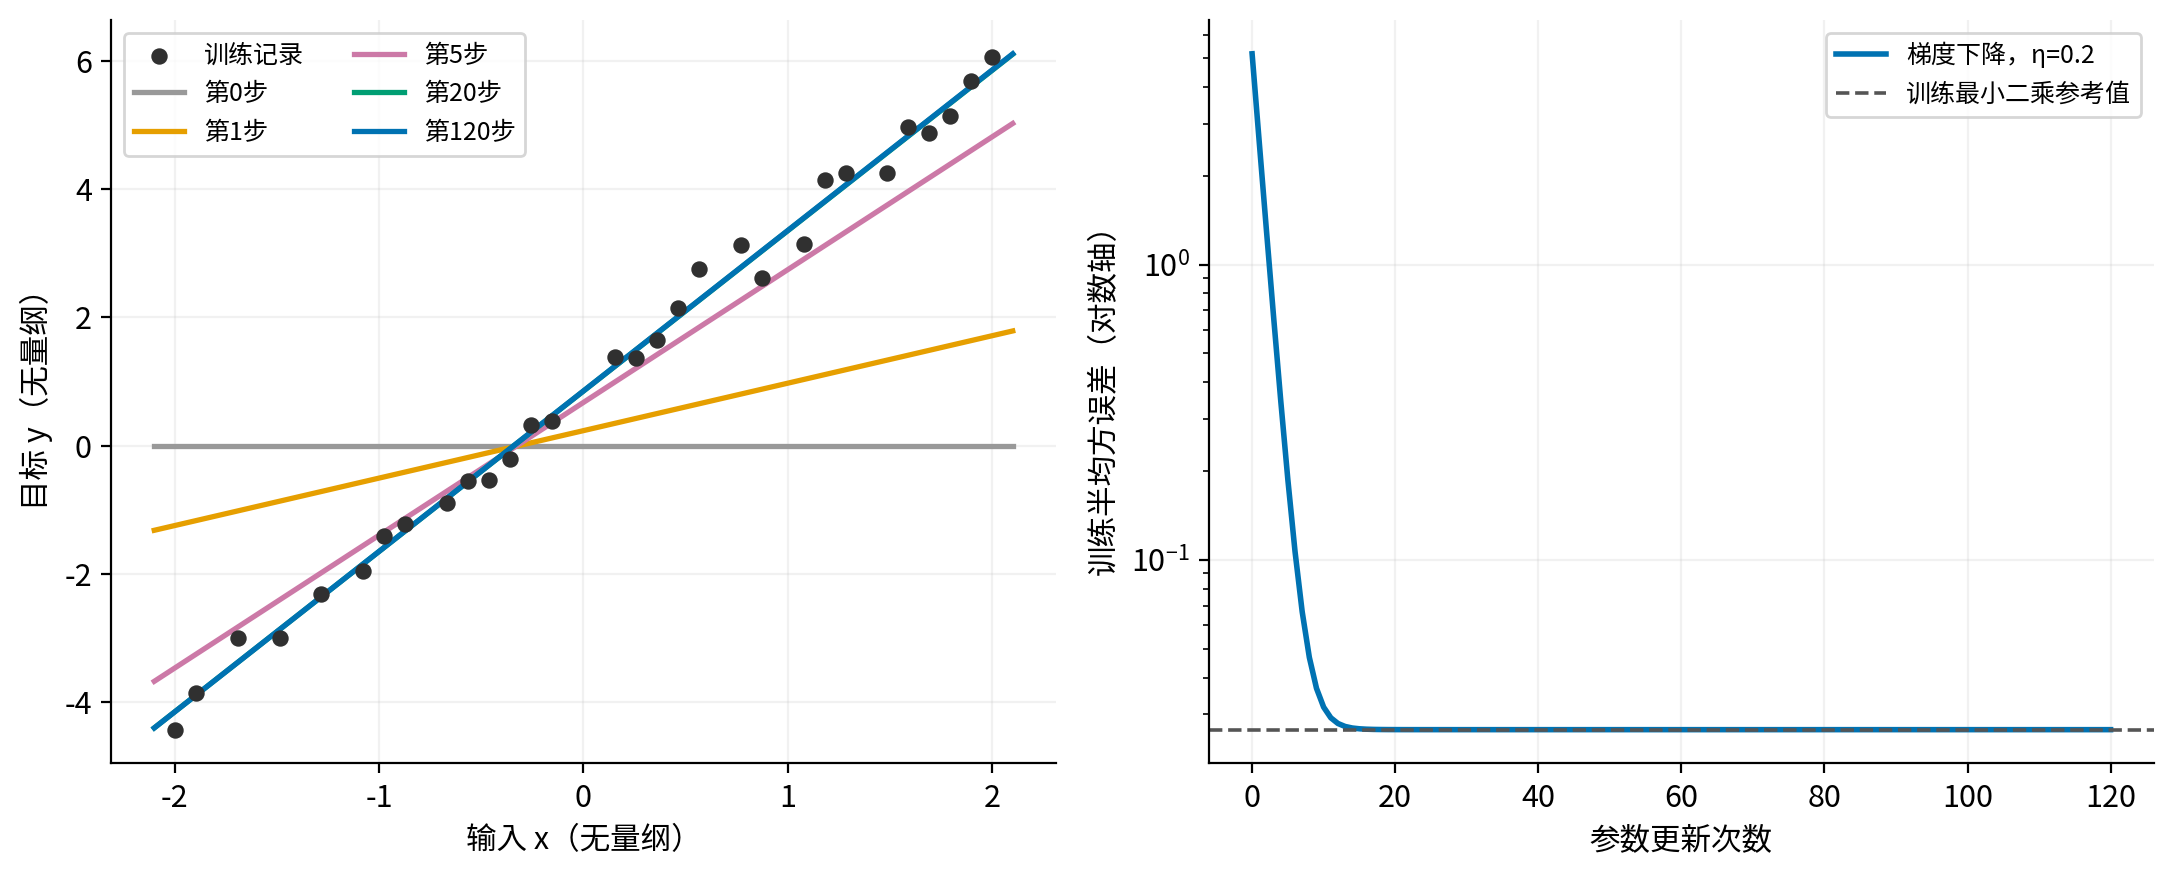
\includegraphics[width=0.92\linewidth]{figures/ch03_figure_3.png}\caption{仅使用固定的30条人工训练记录。左图展示初始状态和若干更新时刻的直线，输入与目标均无量纲；右图展示训练半均方误差及同一训练目标的最小二乘参考值，纵轴为对数轴。参数从 \((0,0)\) 出发，学习率为0.2，共更新120次。}\end{figure}

怎样判断当前低损失是不是因为代码恰好写错了？在这个结构简单的问题上，可以用独立的求解路径作参照。使用 \texttt{LinearRegression} 拟合同样的输入与目标，得到的斜率约为2.506900，截距约为0.853364。手写梯度下降在120步后与其参数的最大绝对差约为 \(1.13 \times 10^{- 12}\)。两种方法共同求解同一个无正则化目标，结果相符支持了本例实现的正确性；这一参照方法并不要求所有机器学习问题都有直接解。

还要区分拟合参数与生成参数。生成式中的斜率和截距是2.5、0.8，而训练得到的是另一组相近数值。这是有限训练样本包含随机噪声的结果。模型寻找的是当前30条记录上的最小损失直线，没有被告知应当直接返回生成式。训练损失不为零也很自然，因为一条直线不能同时穿过全部含噪声的点。已有结果支持``优化过程接近了当前目标的最小值''，尚未检验``在新的观测条件下足够准确''。

\subsection{改变输入尺度之前先预测结果}

接下来把唯一输入改写为 \(u = 1000x\)，仍用直线进行预测。输入包含的信息没有增加，原来能够表达的预测关系也仍然能够表达，只是同一条物理意义上的直线需要用不同的系数表示。我们没有把 \(x\) 与 \(1000x\) 同时作为两个输入特征；那会引出另一种问题。

若沿用学习率0.2，斜率梯度中的输入因子大幅放大，更新迅速越过合适区域。本次运行第2步的训练损失已约为 \(3.26 \times 10^{22}\)，于是触发 \(10^{12}\) 的发散保护阈值。图3-4左图显示的是失败的训练轨迹，不是某种精度更高的拟合。单纯增加更新次数无法消除这样过大的更新步幅。

一种直观补救是把学习率降到 \(10^{- 7}\)。本次运行确实保持稳定，但120步后损失仍约为0.386909，明显高于原问题的最小二乘参考值。换回原始 \(x\) 坐标，斜率约为2.580000，截距却只有约0.000010。这说明为适应斜率方向而选的极小学习率，也让截距方向移动得极慢；``没有发散''与``已经充分训练''并不相同。

另一种办法是用训练数据学习标准化变换。设 \(\mu_{u}\) 和 \(s_{u}\) 分别为训练输入 \(u\) 的均值和标准差，定义新坐标 \(z = \left( u - \mu_{u} \right)/s_{u}\)。这里的标准差按训练记录数 \(n\) 作分母计算，对应 \texttt{StandardScaler} 使用的 \texttt{ddof=0} 约定。{[}4{]} 在本例中，\(\mu_{u} \approx 123.076923\)，\(s_{u} \approx 1192.319640\)。只对训练数据拟合标准化器后，在 \(z\) 坐标中沿用学习率0.2，120步后损失又接近0.02664148。

\begin{figure}[htbp]\centering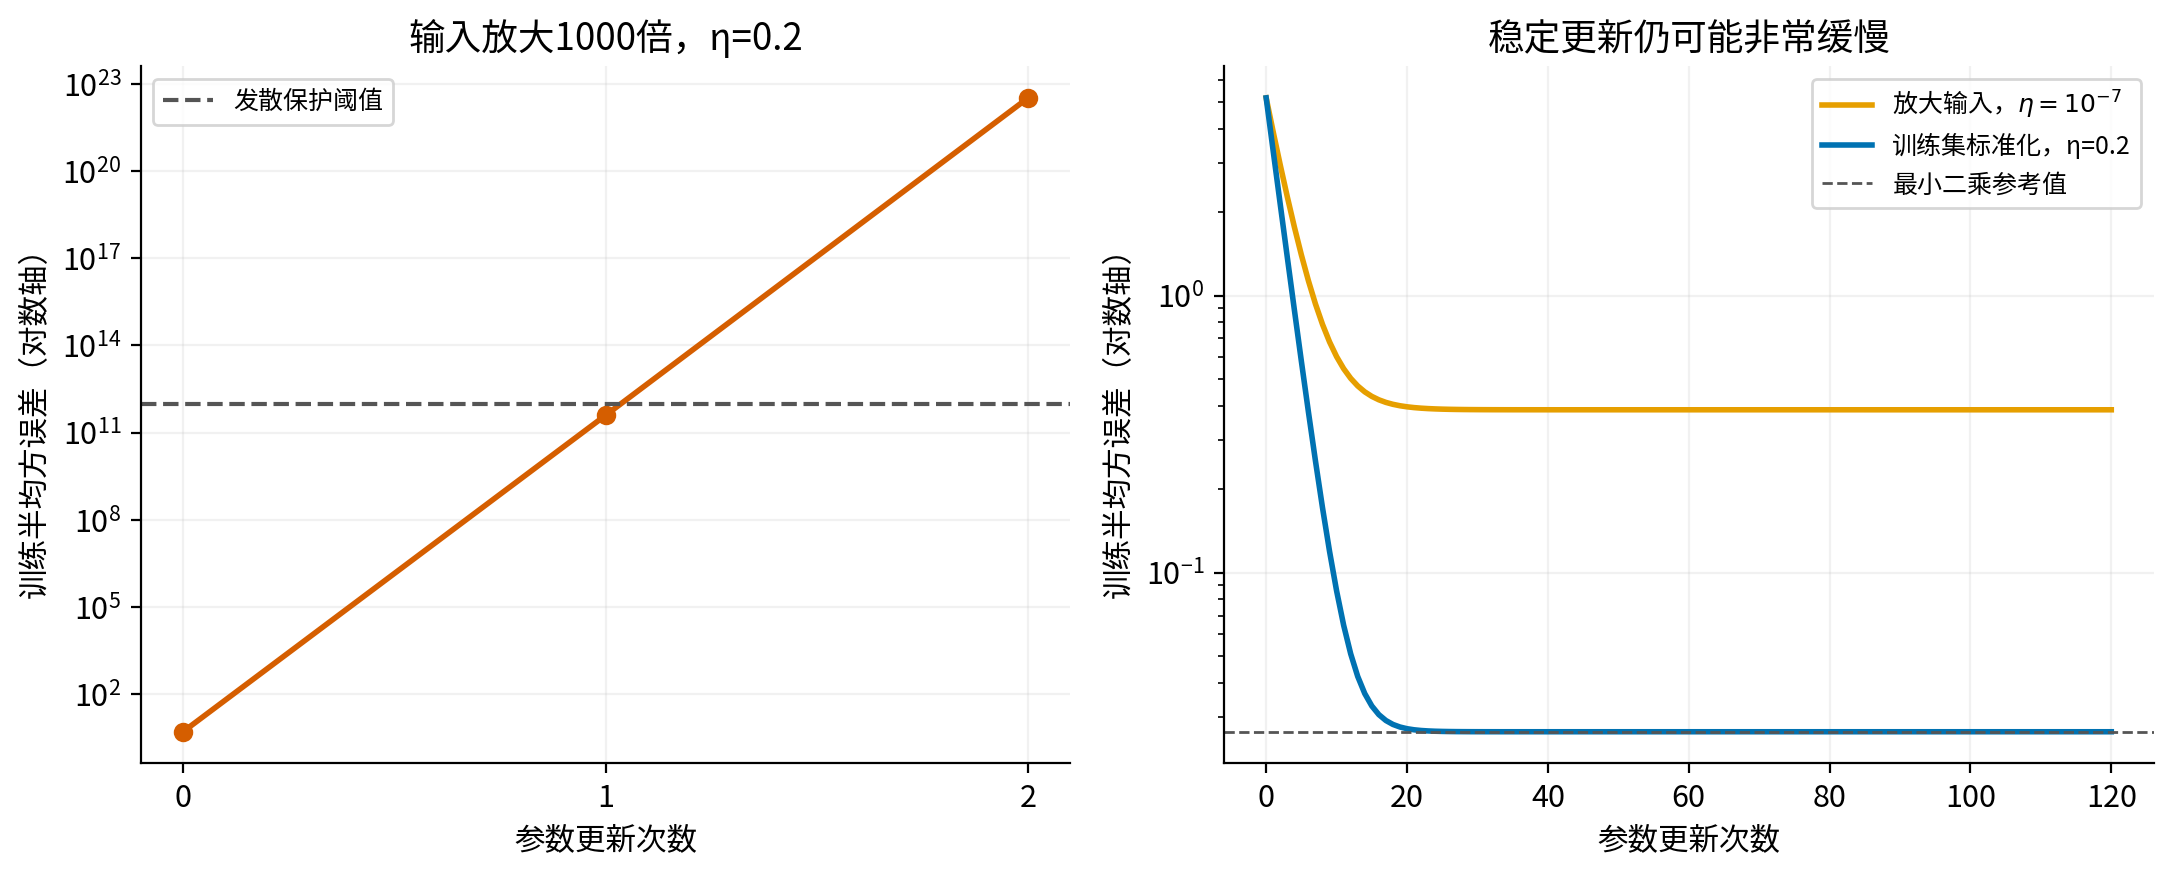
\includegraphics[width=0.92\linewidth]{figures/ch03_figure_4.png}\caption{同一组30条人工训练记录的尺度对照。左图把输入放大1000倍并沿用学习率0.2，在第2步超过发散保护阈值；右图比较放大输入配极小学习率与训练集标准化后的更新。纵轴均为训练半均方误差的对数轴，两幅图范围不同，不能按曲线的视觉高度跨图比较。}\end{figure}

标准化后的系数不能直接与原始坐标的斜率比较。若标准化模型写成 \(\widehat{y} = cz + d\)，其中 \(c\) 和 \(d\) 是新坐标中的斜率与截距，代入 \(z\) 的定义可得：

\[\widehat{y} = \frac{1000c}{s_{u}}x + \left( d - \frac{c\mu_{u}}{s_{u}} \right).\]

因此，原始坐标中的斜率为 \(a = 1000c/s_{u}\)，截距为 \(b = d - c\mu_{u}/s_{u}\)。本次标准化拟合的 \(c \approx 2.989026\)、\(d \approx 1.161905\)，换算后仍得到约2.506900与0.853364。标准化改善了当前优化的数值条件，没有凭空增加数据的信息。这个实验也说明，把不同单位或尺度下的系数数字直接相减，可能会制造没有意义的差异。

\subsection{更换批量方式并解释曲线}

最后，在同一份训练标准化数据上比较三种批量方式。参数都从0开始，学习率都为0.1，均遍历80轮；小批量大小为6，随机打乱种子为42。运行之前，先根据表3-4写出每种方式的更新次数，再预测哪些曲线会更容易出现局部波动。

\begin{figure}[htbp]\centering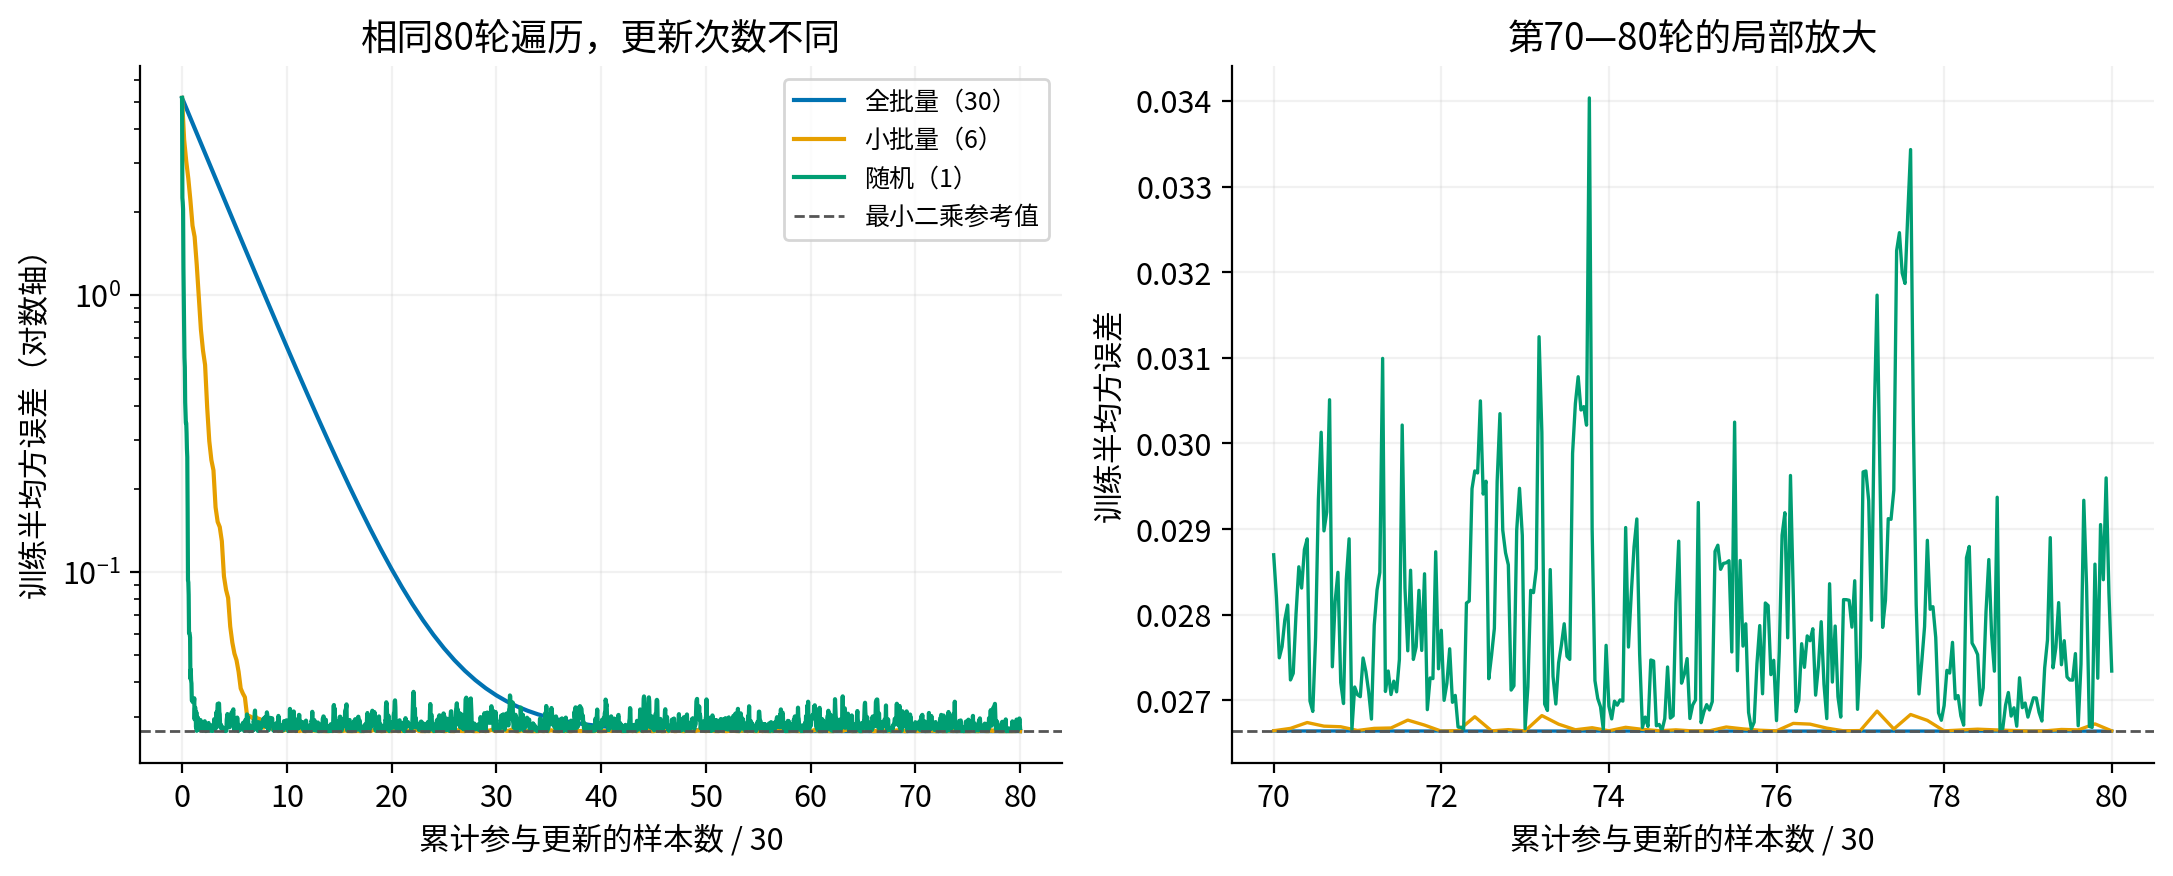
\includegraphics[width=0.92\linewidth]{figures/ch03_figure_5.png}\caption{仅使用30条人工训练记录及由它们拟合的标准化变换。三种方式的常数学习率均为0.1，初值均为0。横轴按累计参与更新的样本数除以30计，整数刻度对应完整遍历轮数；纵坐标始终由全部训练记录计算。右图放大第70至80轮，用于观察最小值附近的波动，不作为运行速度比较。}\end{figure}

图3-5中，单样本更新在相同遍历量内进行了更多次参数调整，早期可以较快靠近较低损失区域；随后仍可看到波动。全批量曲线更平稳，每轮却只走一步。不要用``更平滑''代替``在所有任务中更有效''，也不要用``早期下降快''代替``末步最准确''。它们在这次实验中的差别，是批量大小、学习率和计数方式共同作用的结果。

配套Notebook要求进一步改变打乱种子，观察参数轨迹和末步结果。回答时应明确是哪个目标、哪份数据、哪种计数条件下的现象。例如，可以说``在本次30条训练记录、常数学习率0.1和80轮遍历下，随机更新在最小值附近仍有波动''；不能把一句话缩成``随机梯度下降不收敛''，因为学习率日程、数据特性和训练时长改变后，现象也可能改变。

\subsection{从教学直线走向科学任务}

本实验保留了科学拟合中的几个共同问题：定义输入与目标、选择关系形式、规定误差代价、估计参数并检查残差。若把它迁移到传感器标定，需要进一步讨论量程、系统偏差、重复测量以及不同记录的测量不确定性；若迁移到天文中的经验关系，需要明确样本对象、观测条件和适用范围。我们不会把人工数据上的低训练损失称作某条物理定律得到了验证。

本章的学习结果应当是一条可以解释的链条：参数决定预测，预测产生残差，残差进入损失，梯度描述目标的局部变化，学习率和批量方式规定具体更新，停止条件决定计算何时结束。只会运行最后一行 \texttt{fit} 还不足以说明理解了这条链条；能够借助参数记录解释一条下降或发散的曲线，才为后续模型学习打下了基础。

\subsection{本章练习}

1. 对 \(\widehat{y} = ax + b\)，分别指出输入、监督目标、预测、模型参数和至少三个超参数。如果将学习率从0.2改为0.02，是改变模型表达还是改变优化过程？如果把直线换成二次曲线，又改变了什么？

2. 使用表3-2的三点例子，计算平均残差、MSE与半均方误差，并解释它们的区别。再从 \(a = 1,b = 1\) 出发，用学习率0.3完成一次同步梯度更新，核对新损失。

3. 对示意目标 \(J(w) = (w - 3)^{2}/2\)，从 \(w = 0\) 开始，手算学习率0.5的前两步。再预测学习率2.0的轨迹，运行后说明为什么参数一直变化而损失没有减小。

4. 某程序先更新 \(a\)，然后用新 \(a\) 计算 \(b\) 的梯度。解释它与本章同步更新规则的区别。若这个程序的损失也下降，是否足以证明两者实现相同？

5. 30条训练记录遍历80轮，批量大小分别为30、6和1，各有多少次参数更新？如果另外一个数据集不能被批量大小整除，最后一批的梯度应怎样取平均？

6. 重现尺度实验，解释``大尺度输入与极小学习率''为什么稳定却进展缓慢。把标准化模型的参数换回原始坐标，核对预测是否一致。说明标准化均值和尺度应从哪些记录计算。

7. 保持数据、初值、学习率和轮数不变，把随机打乱种子改为0、1、2、3、4，记录随机与小批量方法的末步训练损失。用结果说明复现一次运行与检查结果波动的区别，不挑选最好的一次代替全部结果。

8. 选择一个熟悉的物理标定或天文经验拟合任务，写出样本单位、输入、目标和拟议模型。列出从本章人工直线迁移过去时，至少三个需要额外检查的问题，并说明为什么训练损失较小不等于科学机制已经成立。

基础提交包括两步参数手算、直线训练记录、学习率和尺度对照图，以及对停止原因的简短解释。批量方式的多种子比较和递减学习率实验可作为进一步探索。教师版Notebook提供参考计算与常见误解的说明。

下一章将暂时放下``怎样继续降低训练损失''，转而建立评价与选择模型的流程。我们会说明怎样使用训练、验证与测试数据，怎样理解过拟合与欠拟合，以及怎样在不接触最终独立测试结果的条件下选择设置。有了这些判断依据，第5章的线性回归、第6章的逻辑回归和第12章的MLP才能放进一套完整而可靠的建模流程中。

\section*{本章参考资料（本章内编号）}

{[}1{]} scikit-learn developers. Stochastic Gradient Descent. 官方用户指南。\url{https://scikit-learn.org/stable/modules/sgd.html} 。关于随机梯度优化、线性估计器及尺度敏感性的说明；本章实际运行版本为scikit-learn 1.8.0，在线stable页面可能随发布更新。

{[}2{]} scikit-learn developers. LinearRegression. scikit-learn 1.8.0 官方API文档。\url{https://scikit-learn.org/1.8/modules/generated/sklearn.linear_model.LinearRegression.html} 。关于最小二乘拟合、构造选项与拟合后系数属性的说明。

{[}3{]} scikit-learn developers. Common pitfalls and recommended practices. scikit-learn 1.8.0 官方用户指南。\url{https://scikit-learn.org/1.8/common_pitfalls.html} 。关于先划分数据、仅在训练部分学习预处理变换及保持变换一致性的说明。

{[}4{]} scikit-learn developers. StandardScaler. scikit-learn 1.8.0 官方API文档。\url{https://scikit-learn.org/1.8/modules/generated/sklearn.preprocessing.StandardScaler.html} 。关于训练均值、尺度及标准差计算约定的说明。

本章数据、表格及数值结果均由配套 \texttt{build\_experiments.py} 实际生成和计算。固定环境、数据字段、运行记录及完整实验位于随章材料；正文取舍以机制解释为主，完整作图与循环代码保留在Notebook中。

\section*{深化练习与方法检验}
本组题强调解释、计算与验证；D编号在本章内独立计数。计算题应写出所用定义和中间步骤，实验题保留实际输出，包括不支持预期的结果。
\begin{enumerate}[label=D\arabic*.]
\item 给定 $J(\theta)=\frac12(4\theta_1^2+\theta_2^2)$，从 $(1,1)$ 出发，以学习率0.2完成一步更新。求常数学习率使任意非最优初值收敛所需的区间，并指出其依据。
\item 将平均平方误差乘以正数5。最优参数、梯度、保持相同更新轨迹所需的学习率分别怎样变化？加入正则化项但不同时缩放其系数时，最优参数是否仍必然不变？
\item 说明“用一个小批量的平均损失估计完整梯度”这句话错在哪里。怎样在合适的随机抽样条件下写出正确的无偏性关系？
\item 某损失曲线几乎水平。提出三种不同解释，并给出能区分它们的进一步检查。
\end{enumerate}

\chapter{模型评价、选择与泛化}
\label{chap:evaluation}
\chaptergoal{能区分学习参数、选择方案和最终检查的用途；能从具体预测记录计算分类与回归指标；能解释基线、欠拟合、过拟合和交叉验证；能把数据处理与模型放在同一验证流程中。}

第3章说明参数怎样改变、训练损失怎样下降。现在需要回答另一个问题：学到的规则遇到新记录时是否仍然有用？把训练记录全部记住并不等于能处理新的对象。本章先讨论怎样留出用于检查的记录，再讨论怎样把预测好坏写成数值，最后将评价用于模型选择。

本章继续使用第2章介绍的葡萄酒数据：每条记录是一份酒样的13项分析指标，目标为三类来源。选择熟悉的数据，是为了把注意力放在评价过程，而不是同时适应新的研究对象。住房回归只作为已介绍的连续目标任务进行对照。

\section{训练、验证与独立测试}
\subsection{三种用途，不是三种文件格式}
\textbf{训练集（training set）}用于确定模型参数或其他预测规则。\textbf{验证集（validation set）}用于比较候选算法、预处理方式与参数配置。\textbf{测试集（test set）}是在方案确定后，用来检查新样本表现的数据。前两者共同组成开发过程；“独立测试”强调测试信息没有反过来参与方案选择。

可以把开发过程想成先做练习，再用一套模拟题选择学习策略，最后参加不用于改策略的考试。训练集对应用于形成规则的练习，验证集帮助选择规则，测试集用于最终检查。关键是信息怎样流动，而不是变量名怎样命名：反复根据某个所谓测试集改模型，它实际上已经承担验证用途。

\subsection{一个有记录数的划分例子}
假设有100条适合按独立样本随机划分的记录，可以先留20条作最终测试，余下80条用于开发。再把开发数据分成60条训练、20条验证。训练三个候选方案时，每个方案都只用相同的60条记录建立规则，再在相同20条验证记录上比较。选定方案后，可以按预先约定在全部80条开发记录上重新拟合，最后在最初保留的20条上评价。

60、20、20只是解释角色的人工例子，不是必须采用的比例。实际葡萄酒数据有178条，以下代码先留约20\%，得到142条开发记录和36条最终保留记录；开发部分内部再用交叉验证，详见4.5节。
\begin{lstlisting}[caption={建立后续章节共用的开发与保留划分}]
from sklearn.datasets import load_wine
from sklearn.model_selection import train_test_split
wine = load_wine(as_frame=True)
X_dev, X_test, y_dev, y_test = train_test_split(
    wine.data, wine.target, test_size=0.20,
    random_state=42, stratify=wine.target
)
print(len(X_dev), len(X_test))
\end{lstlisting}

\textbf{分层划分}尽量保持类别比例，避免偶然把某个少数类几乎全部分到一边。\textbf{分组划分}则按对象或实验组分配记录，例如同一天体的重复观测进入同一部分。\textbf{时间划分}按先后顺序检查对未来的预测。三者解决的不是同一个问题，选择应对应预期应用，而非机械地一律随机拆行。
\fig{ch04_split.pdf}{开发数据、内部验证与最终测试的角色。最终测试不是另一次用来挑选最好参数的验证。}

\subsection{一套固定口径贯穿后续实验}
本书新增的标准实验统一先按种子42保留20\%作为最终测试；剩余数据称为开发集。算法比较主要采用开发集上的五折分层交叉验证，折划分种子为7。为绘制训练曲线或追踪一个样本，某些实验再把开发集按种子7划分为75\%训练和25\%验证。两种实验分别标为“五折比较”和“固定验证示范”，不能把它们的分数当作同一条件的重复测量。

对鸢尾花，固定示范有90条训练、30条验证，另30条最终保留；对葡萄酒，有106条训练、36条验证，另36条最终保留。小数比例经程序取整，所以记录数比单纯报告百分比更准确。拆分索引保存在随书CSV中，之后各章无需重新随机寻找一个更好看的划分。

在初学阶段，保留测试数据的价值不只是“获得一个最终分数”，还在于让模型选择和评价的职责分开。若课程已经围绕某个标准数据反复教学多年，它不再是研究意义上完全陌生的新数据，但仍可用来练习正确流程。真实科学报告需要另外考虑数据选择历史，不能把课堂保留方式当作自动消除所有研究偏差的办法。

\subsection{按对象划分与按行划分回答不同问题}
随书构造了一个可以精确检查的反例。90个模拟对象各有5次测量，每个对象具有一个随机生成的8维“指纹”，同对象的重复测量只加入很小扰动；对象类别则独立随机生成，与指纹之间没有总体规律。一个最近邻规则在随机拆行时，可以从训练中找到几乎相同的对象记录；按对象拆分时则不能。

实际五折运行中，按行划分每折准确率都是1.0；按对象划分的五折准确率约为0.611、0.667、0.533、0.444、0.522。前者并非发现了随机类别的物理规律，而是利用了同对象的近重复记录。后者围绕机会水平波动，符合本人工构造没有跨对象预测信息的设置。

\fig{v3_ch04_groups.pdf}{同一人工数据的两种验证问题。按行拆分评估对已见对象的重复测量，按对象拆分评估新对象。两条曲线不能被解释为同一任务下两种算法的优劣。}
这个反例的结论不是“所有随机划分都有错”，而是\textbf{评价中的新样本必须与实际应用中的新样本含义一致}。若使用目标确实是预测已知对象的新测量，重复信息可能是允许的；若声称预测从未出现的对象，就必须相应隔离对象身份。

\section{分类与回归的评价指标}
\subsection{先数清楚哪些记录被分错}
\textbf{评价指标（metric）}是按明确规则把一批预测结果汇总为数值的方式。分类最直观的指标是\textbf{准确率（accuracy）}，即判断正确的记录数除以总数。为了知道错在哪一类，可以制作\textbf{混淆矩阵（confusion matrix）}：行表示参考类别，列表示预测类别，每个格子统计对应记录数。

考虑人工构造的10条二分类记录，把关注的类别称为正类，其余称为负类。“正”不是好、“负”不是坏，只是为了明确统计对象。表\ref{tab:confusion-hand}给出一组预测结果。
\begin{table}[htbp]\centering
\caption{用于手算的10条二分类记录汇总，不是实际观测结果。}\label{tab:confusion-hand}
\begin{tabular}{lrrr}\toprule
&预测为正&预测为负&合计\\\midrule
实际为正&3（TP）&1（FN）&4\\
实际为负&2（FP）&4（TN）&6\\\midrule
合计&5&5&10\\\bottomrule
\end{tabular}\end{table}

\textbf{真阳性TP}表示实际为正且预测为正；\textbf{假阳性FP}表示实际为负却报成正，也称误报；\textbf{假阴性FN}表示实际为正却判成负，也称漏检；\textbf{真阴性TN}表示实际为负且预测为负。先按实际与预测的两种状态定位格子，再记名称，就不容易混淆。

本例准确率为 $(3+4)/10=0.7$。如果关注预测为正的候选有多少可信，计算\textbf{精确率（precision）}：$3/(3+2)=0.6$。如果关注所有真正正类中找回多少，计算\textbf{召回率（recall）}：$3/(3+1)=0.75$。一般式为
\[
\mathrm{Precision}=\frac{\mathrm{TP}}{\mathrm{TP}+\mathrm{FP}},\qquad
\mathrm{Recall}=\frac{\mathrm{TP}}{\mathrm{TP}+\mathrm{FN}}.
\]
\textbf{F1分数}是二者的调和平均，在分母非零时为
\[
F_1=\frac{2\,\mathrm{Precision}\,\mathrm{Recall}}{\mathrm{Precision}+\mathrm{Recall}}
=\frac{2\mathrm{TP}}{2\mathrm{TP}+\mathrm{FP}+\mathrm{FN}}.
\]
本例为 $6/9=2/3$。分母为零时，应声明采用的软件约定，不能把未定义的情况当作有科学意义的零或满分。

\subsection{多分类与类别不平衡}
鸢尾花或葡萄酒有三个类别，混淆矩阵就是三行三列。逐类别计算召回率时，把当前类别视为正，其余合为负。\textbf{宏平均（macro average）}是先分别计算各类指标，再对类别等权平均；\textbf{加权平均}按各类样本数加权。类别很少的对象在两种汇总中的权重不同，报告时要说明选择。

例如1000条记录只有10条关注对象，一个全部预测为背景的规则准确率为99\%，却没有找回任何关注对象。这样的\textbf{类别不平衡}说明仅看准确率不够。指标应回答实际问题：漏掉对象的代价大，还是后续检查大量误报的代价大？
\fig{ch04_confusion.pdf}{鸢尾花的三分类混淆矩阵实例。对角线是判断正确的数量，非对角线给出具体的误判方向。}

\subsection{回归误差需要带着单位解释}
对回归，用 $e_i=\hat y_i-y_i$ 表示第 $i$ 条预测残差。\textbf{平均绝对误差MAE}先取绝对值再平均；\textbf{均方根误差RMSE}先平方取平均，再开平方：
\[
\mathrm{MAE}=\frac1n\sum_i|e_i|,\qquad
\mathrm{RMSE}=\sqrt{\frac1n\sum_i e_i^2}.
\]
假设人工给出目标 $(2,4,6)$ 与预测 $(3,4,5)$，残差为 $(1,0,-1)$。于是MAE为 $2/3\approx0.667$，RMSE为 $\sqrt{2/3}\approx0.816$。二者都具有目标的单位；平方再开根使较大的残差在RMSE中受到更明显的影响。

\textbf{决定系数 $R^2$}比较平方误差与以评价样本目标均值为常数的参照：
\[
R^2=1-\frac{\sum_i(y_i-\hat y_i)^2}{\sum_i(y_i-\bar y)^2}.
\]
上例 $\bar y=4$，分母为8，分子为2，所以 $R^2=0.75$。这不是“75\%的样本预测正确”。它可以为负，表示比该常数参照更差；目标完全不变时分母为零，需要另行处理。注意，此处评价样本均值只用于定义指标，真正可部署的常数预测器必须从训练目标估计常数，不能提前获取新样本目标\textsuperscript{[32]}。

\subsection{从混淆矩阵推到误报率和样本比例}
精确率的分母是所有被报为正类的记录，召回率的分母是真正的正类；\textbf{假阳性率}则是$\mathrm{FP}/(\mathrm{FP}+\mathrm{TN})$，分母是真正的负类。三者不能替换。对于极少见的对象，负类数目很大，即使假阳性率不高，也可能产生大量误报。

\worked{稀有对象筛选中的基数效应}
假设10万条记录中只有100条目标，模型召回90条目标，即召回率0.9。若假阳性率为0.01，则99900条背景中约有999条被误报，候选总数约1089，精确率只有$90/1089\approx0.0826$。这组数字是任务设定的算例，不是实际天文调查结果。

若模型在一个正负各半的评估集上表现很好，也不能直接把该集的精确率照搬到目标比例千分之一的巡天。预测概率的校准、类别比例以及后续核查预算都要重新考虑。这个例子解释了为什么候选筛选报告必须同时给出样本规模、类别比例、召回率和误报信息。

\subsection{阈值变化形成一组评价点}
概率分类器通常给出一个连续分数，把它转成类别需要阈值。逐渐降低阈值，报告的候选集合通常扩大；TP和FP都不会因集合扩大而减少，但精确率不保证单调。第6章将逐条计算一个阈值例子。ROC曲线以假阳性率为横轴、召回率为纵轴；PR曲线以召回率和精确率描述不同阈值的取舍。曲线概括排序行为，却不能替应用者决定最终阈值。

面积指标也不是一个应用阈值。例如较好的整体排序仍可能在高纯度要求的区域表现不足。对于科学候选目录，可以事先规定“人工最多核查50个对象”或“允许的误报预算”，然后在开发数据上选择满足目标的操作点，而不是仅凭曲线面积宣布模型足够好。

\subsection{同一个回归误差，可以有不同科学后果}
RMSE对大偏差更敏感，MAE较直接地报告典型绝对偏差。若误差单位是十万美元，数值0.4代表4万美元；若目标先取了对数，则对数误差需要转换后才能解释为原单位的相对偏差。不同目标变换后的分数不能直接排在同一表格里比较大小。

对于不确定度不同的观测，可以另外检查标准化残差$e_i/\sigma_i$，其中$\sigma_i$必须是明确来源的测量不确定度或预测尺度。它不是把误差“消除”，而是在相应噪声假设下比较偏离程度。\textbf{不能为使标准化残差看起来正常，事后任意调大分母。}本课程的主线先报告原单位误差，第16章再区分误差来源。

\worked{RMSE为什么不小于MAE}
对残差绝对值$a_i=|e_i|$，有
\[
\frac1n\sum_i a_i^2-\left(\frac1n\sum_i a_i\right)^2
=\frac1n\sum_i(a_i-\bar a)^2\ge0.
\]
两边开平方得到$\mathrm{RMSE}\ge\mathrm{MAE}$。只有所有残差绝对值相同时等号成立。这个短推导帮助检查程序：若同一批、同一权重的记录上报告RMSE小于MAE，应先核对实现、单位或数据范围，而不是急于解释模型。

\section{基线模型与公平比较}
\textbf{基线（baseline）}是用于比较的简单或已有方案。它提供“比什么更好”的参照。例如分类时始终报训练集中最多的类别，回归时始终报训练目标均值。它们未必足够好，却能检查一个复杂模型是否真的利用了输入信息。

假设训练分类记录中A占70\%，B占30\%，多数类基线对所有新输入都报A。新记录如果恰有同样比例，该基线也能有70\%准确率；所以得到71\%需要结合波动判断，不能单凭模型名称就称为显著进步。对于回归，训练目标为2、4、6时，均值基线给所有新输入报4。

sklearn提供 \texttt{DummyClassifier} 和 \texttt{DummyRegressor} 实现这类参照。\texttt{Dummy}在这里表示不利用复杂输入关系的简单规则，不是虚构数据。
\begin{lstlisting}[caption={先建立能解释清楚的多数类基线}]
from sklearn.dummy import DummyClassifier
from sklearn.model_selection import StratifiedKFold, cross_val_score
cv = StratifiedKFold(n_splits=5, shuffle=True, random_state=7)
baseline = DummyClassifier(strategy="most_frequent")
scores = cross_val_score(baseline, X_dev, y_dev, cv=cv, scoring="accuracy")
print(scores, scores.mean())
\end{lstlisting}

\textbf{公平比较}要求所比较方法面对相同的任务、样本范围、可用特征和评价划分。不同方法可以采用适合自身的预处理，但变换必须在各自训练范围内学习。若新模型同时增加了原模型没有的高质量测量，结果改善不能全部归因于算法。

\subsection{基线也要在每一折中重新拟合}
回归常数基线的均值来自当前训练目标，分类多数类来自当前训练标签。交叉验证中每折训练部分不同，基线参数也要重新确定。若预先使用全部数据的目标均值作为所有折的预测常数，验证信息已经影响了基线。虽然这种影响可能不大，完整比较仍应统一规则。

公平比较还需要限制可获得的信息和调参投入。例如模型A仅使用两个测量，模型B使用额外十个高精度测量，分数差异同时包含信息差异和算法差异。可以分别设置“同特征比较”和“增加信息比较”，而不是把二者混为一种进步。同理，一个模型搜索1000组配置，另一个只用默认配置，其结果既反映模型也反映开发投入。

\subsection{配对比较比只看两个平均数更有信息}
在完全相同的五折上评价模型A和B，可以计算每折差值$d_k=s_{A,k}-s_{B,k}$。若两模型分别在不同随机划分上得到平均0.95和0.96，无法判断差异主要来自模型还是验证样本难度。固定折至少可以让两者面对相同的难题。

但折间训练数据重叠，所以五个差值也不是五次完全独立的重复实验。对于本课程，先报告各折值、均值、差值方向和实际误判数量；不把微小平均差异自动写成统计显著。若需要正式比较，应依据对象相关结构和研究设计选择额外检验或重采样方法。

随书葡萄酒五折实验同时记录多数类基线和标准化逻辑回归。后者的作用此时只是一个提供好的候选规则，第6章再解释内部原理。不要因为它的名称更复杂而预先判断一定优于基线；先看同一折的实际结果。

\section{欠拟合、过拟合与模型复杂度}
\textbf{欠拟合（underfitting）}指当前模型或训练过程未充分表达数据中可学习的关系，常见表现是训练和验证误差都较大。\textbf{过拟合（overfitting）}指模型过度适应训练样本中的偶然细节，使训练改善没有转化为新样本上的改善。两者描述的是相对于任务、样本和训练过程的行为，不是固定的算法标签。

例如真实关系明显弯曲，模型却只允许一条直线，那么反复优化直线的斜率可能仍留下系统残差；这是表达能力不足的例子。如果允许一条曲线穿过每一个含噪测量点，它可能在训练点间剧烈弯折，对新测量反而预测更差；这是过度适应训练细节的例子。

\textbf{模型复杂度}描述规则表达多样关系或适应细节的能力，不能在所有算法间只用同一个数字衡量。后面的树模型通过增加条件分支形成更细的规则，神经网络通过增加计算单元改变表达能力。第3章的正则化则通过惩罚过大的参数施加限制。

图中树深可以先理解为沿一条判断路径允许进行多少层条件判断，具体树结构在第8章展开。曲线横轴改变复杂度，纵轴分别检查训练和验证结果；选择应以验证任务为依据，而不是只追求训练曲线最高。
\fig{ch04_tree_complexity.pdf}{条件判断层数增加时，训练与交叉验证表现可能不同。图中的树模型将在第8章解释，本章关注如何读两条评价曲线。}

\subsection{优化不足与表达不足不是同一问题}
训练误差高可能因为模型形式太简单，也可能因为参数还没有充分优化，还可能因为输入本来不含足够信息。三种情形的处理不同：增加训练轮数可能解决优化不足，却不能让一条直线变成弯曲函数；增加模型复杂度可能改善表达，却不能恢复未被测量的关键变量。

可以先对一个小训练子集检查模型是否能拟合，再查看训练目标的下降曲线和停止信息。如果小子集也学不好，先检查代码、数据配对、尺度和优化；如果训练可以非常好而验证差，才更有理由讨论过拟合和分布差异。这个诊断顺序在第12章神经网络中尤其重要，但也适用于其他模型。

\subsection{学习曲线和复杂度曲线}
复杂度曲线在固定数据量下改变模型配置；\textbf{学习曲线}在固定配置下改变训练样本量。两者横轴不同，不能混称。训练量增加时，训练分数可能下降，因为模型不能再只适应极少数记录；验证分数可能提高，也可能在模型形式受限时很快达到平台。

如果训练和验证误差都高且接近，继续收集相似样本未必解决表达不足；如果训练好、验证差且差距随样本增多而减小，增加数据可能有帮助。这些是诊断线索，不是仅凭曲线形状就能下的唯一结论。不同样本质量、划分方式和目标噪声也会改变曲线。

\subsection{选读：偏差与方差的一个精确分解}
假设$Y=f_*(x)+\varepsilon$，固定输入$x$，噪声满足均值零、方差$\sigma^2$，且与训练集独立。用随机训练集$D$得到预测$\hat f_D(x)$，记平均预测为$\bar f(x)=\mathbb E_D\hat f_D(x)$。将误差加减$\bar f$并展开，交叉项期望为零，得到
\[
\mathbb E_{D,\varepsilon}(Y-\hat f_D(x))^2
=\bigl(f_*(x)-\bar f(x)\bigr)^2
+\mathbb E_D\bigl(\hat f_D(x)-\bar f(x)\bigr)^2+\sigma^2.
\]
第一项是平均预测的偏离，第二项是训练数据变化导致的预测波动，第三项是这个输入信息下的随机噪声。这个等式需要上述假设，也只针对平方误差。它解释随机森林为什么关注降低预测波动，但不意味着在每个真实任务中可以从一套数据精确估计三项。

\section{交叉验证及结果波动}
\textbf{$K$折交叉验证（$K$-fold cross-validation）}将开发数据分为 $K$ 份，每次留一份验证，用其余份重新训练，轮流完成 $K$ 次。每一份称为一折。这里的 $K$ 是验证分组数，与第7章近邻算法的邻居数无关。

用12条人工编号记录说明三折验证：第一轮用5--12号训练、1--4号验证；第二轮用1--4和9--12号训练、5--8号验证；第三轮用1--8号训练、9--12号验证。每轮都重新建立模型与处理规则，不是让一个模型依次见到全部记录后再声称轮流验证。
\fig{v2_cross_validation.pdf}{12条人工编号记录的三折验证。每一行是一轮独立拟合，标出的验证部分在该轮不参与参数学习。}

若三轮准确率为0.75、1.00、0.75，平均值为 $2.5/3\approx0.833$。折间差异说明本次结果随划分变化，但这些训练部分相互重叠，折间标准差不是自动成立的置信区间。正式数据量与类别比例可能不同，也不应把三折手算数字写成葡萄酒实验结果。

\texttt{StratifiedKFold}尽量保持每折类别比例；\texttt{GroupKFold}按事先定义的对象组划分。一个材料有多次重复测量时，目标若是预测新材料，就不能把同一材料的重复测量同时放进训练与验证。只固定随机种子不能解决这种相关性问题。

\subsection{不相等的折大小与两种平均}
若一折验证20条、错2条，另一折验证30条、错6条，则两折准确率分别为0.9和0.8。简单折平均为0.85，把两折全部预测汇总后准确率为$(18+24)/50=0.84$。二者都可以计算，但含义不同。样本数几乎相等的普通$K$折中差别较小，按对象或时间分块时则可能明显。

对F1等非线性指标，先汇总混淆矩阵再计算，与先算各折指标再平均，也不一般相等。报告要写清采用哪种汇总。随书算法比较主要使用各折分数的算术平均，同时保存每折值；项目报告可以额外报告合并的折外预测指标，但应注明。

\subsection{嵌套验证：评价一个选择过程}
假设希望比较多个算法和参数，内层交叉验证可以负责选择；外层把一部分开发数据完全留出，用于检查内层选择流程的表现。每个外层训练部分都重新完成填补、缩放、调参和模型选择，再预测相应外层验证部分。这叫\textbf{嵌套交叉验证}。

它评价的是“按这套方法挑模型”这一过程，而不是某个事后挑出的固定参数。代价是拟合次数增加。小型课程练习可以采用固定测试集加内层验证，不强制每章嵌套；当报告涉及较多选择时，应理解为什么直接汇报最高内层分数容易乐观。

分组或时间约束要同时落实到内外两层。只在外层隔离天体，内层却按重复观测随机拆行，仍可能选出依赖对象重复信息的方案。验证设计是整个流程的属性，不是只改一个最后调用就能保证。

\section{超参数选择与模型选择}
第3章区分了参数与超参数。参数在训练中由数据学习，超参数是指定算法如何学习的配置，例如允许的树深、正则化强度或邻居数量。\textbf{模型选择}是根据验证结果在算法、特征处理和配置之间作出选择。

\textbf{网格搜索（grid search）}把少量候选值列成组合，逐个验证。例如配置A在三折得到 $(0.75,0.75,1.00)$，配置B得到 $(0.75,1.00,1.00)$，可以按事先规定的平均准确率偏向B；但这只是开发阶段选择，并不证明B在所有未来记录上都更好。最终保留数据用于提供额外检查。

后面的逻辑回归用 \texttt{C} 控制正则化相关配置，第6章解释它的作用。这里把它当作三个候选规则的配置标记即可，不需要提前掌握模型细节。\texttt{GridSearchCV}负责在开发数据上重复拟合并记录验证结果。
\begin{lstlisting}[caption={把候选配置限制在开发数据中比较}]
from sklearn.linear_model import LogisticRegression
from sklearn.preprocessing import StandardScaler
from sklearn.pipeline import Pipeline
from sklearn.model_selection import GridSearchCV
pipe = Pipeline([
    ("scale", StandardScaler()),
    ("clf", LogisticRegression(max_iter=2000))
])
search = GridSearchCV(pipe, {"clf__C": [0.1, 1.0, 10.0]},
                      cv=cv, scoring="accuracy")
search.fit(X_dev, y_dev)
print(search.best_params_, search.best_score_)
\end{lstlisting}

变量名 \texttt{clf\_\_C} 用双下划线连接步骤名和参数名。最高验证分数已经参与了方案选择，不能再把它标成未参与选择的测试分数。选择越多、越频繁地依据同一验证数据修改方案，越需要警惕对验证结果的偶然适应。

\subsection{从有限搜索到可解释的选择}
入门实验应该让每个候选值有理由。例如近邻数从1、3、5到较大的值，分别考察局部敏感与更强平滑；树深从1、2到更深，考察条件规则增加的效果。初次学习不宜把所有参数笛卡尔积组合成数千次搜索，因为学生很难解释每个变化。

选择准则也应事先确定。可以优先平均召回率，但要求精确率达到下限；可以优先RMSE，在差异很小的方案中选较简单或较便宜者。训练速度和预测成本同样可以记录，不过不同算法的运行条件必须一致。不能先看所有指标，再挑一个恰好支持自己偏好的结论。

\worked{选择后的分数为什么可能偏高}
假设十种实际能力相近的方案，在同一小验证集上的分数都包含随机波动。选择其中最高者，往往同时选中了正向波动较大的一次。这不需要某个算法有错误，也不需要故意作弊；只要“取最大值”，就可能产生选择偏差。另一个没有参与选择的数据集能够检查这个乐观程度。

提高实验可以人工生成完全随机的目标，增加候选模型数，观察最高验证分数怎样变化。该实验的意义是理解选择过程，不是说明真正数据中的所有高分都是假的。只有把目标设为随机、保持构造方式透明，才知道基准情形是什么。

\section{Pipeline与可复现的评价流程}
\subsection{流水线怎样避免漏掉处理步骤}
第2章已经手动分开了标准化的学习与应用。\textbf{Pipeline}将这些步骤与预测模型组成一个对象。在一次交叉验证中，程序先在当前训练折学习均值、尺度等规则，再训练模型；验证折只经过已经学习的变换和预测。下一折重新拟合整个流程，而不是沿用上一折的均值。

以上代码中的 \texttt{scale} 是标准化步骤的名称，\texttt{clf} 是分类模型步骤的名称。调用流水线 \texttt{fit} 时依次完成拟合与变换；调用 \texttt{predict} 时，对新数据应用同一预处理再预测。它不能自动阻止所有错误，例如一开始把目标列放进输入仍然会泄漏，但可以减少常见的预处理越界问题\textsuperscript{[3,4]}。

\subsection{什么叫可复现}
\textbf{可复现}在本书指另一位读者能依据记录的材料、软件和步骤，重新得到可核对的实验结果。至少保存数据来源、筛选条件、拆分索引、模型配置、软件版本、随机状态和评价代码。随机种子只固定部分随机过程，不保证跨版本完全相同，也不能代替稳定性检查。

完成一项预测实验后，应能回答：哪些记录用于学习参数，哪些用于选择方案，哪些直到最后才打开？某张图是训练结果还是验证结果？代码中的分数是单折、折均值还是最终保留结果？这些标注比一串小数位更重要。

\subsection{把实验记录写成可以复算的对象}
一个模型比较表至少包含：任务与目标单位、数据版本、开发与保留划分、特征列表、预处理、模型配置、指标及各折结果。不要只保存截图，因为截图通常不能恢复误判样本是谁。对应预测表应保留记录标识、参考目标、预测结果，以及必要的概率或残差。

流水线对象可以保存已经学习的处理规则，但不应替代清晰的代码和数据字典。模型文件由软件序列化产生，读取不可信来源的序列化对象可能执行代码，因此教学交付优先提供源码、数据和重训方式，不要求学生随意加载未知模型文件。

本书把“程序能够执行”“数值与手算一致”“验证设计回答正确问题”分开检查。第一项发现语法和依赖错误；第二项检查计算实现；第三项检查科学和统计设计。任何一项通过，都不能自动替代另外两项。这样的区分将在最后的项目评审中继续使用。

\chapterpractice{手算表\ref{tab:confusion-hand}的准确率、精确率、召回率和F1；计算三点回归例子的MAE、RMSE与$R^2$。用葡萄酒开发数据完成多数类基线与一个已提供候选模型的交叉验证，记录各折与均值，暂不反复查看最终测试。}
\chapterexercise
\begin{enumerate}
\item 把10条人工记录中一个假阳性改成真阴性，准确率、精确率和召回率分别怎样变化？
\item 训练、验证、测试三种用途能否仅凭文件名区分？举一个测试数据被用于选择方案的例子。
\item 对目标 $(2,4,6)$ 和预测 $(2,4,8)$，计算MAE与RMSE，并解释单位。
\item 写出12条记录三折验证的训练与验证编号。每轮为什么需要重新计算标准化参数？
\item 为什么在同一天体的重复观测之间随机拆行，不能直接代表对新天体的预测能力？
\end{enumerate}

\section*{深化练习与方法检验}
本组题强调解释、计算与验证；D编号在本章内独立计数。计算题应写出所用定义和中间步骤，实验题保留实际输出，包括不支持预期的结果。
\begin{enumerate}[label=D\arabic*.]
\item 两模型在同一100条验证记录上准确率分别为0.90和0.92。仅凭这两个数能否判断第二个模型的改善稳定？还应保存哪些逐记录信息，怎样设计进一步比较？
\item 真实正类占1\%，分类器召回率0.9、负类误报率0.05。以10000个对象计算预期真阳性、假阳性和精确率。解释为什么总体准确率不能代替候选清单的纯度。
\item 先在全部开发数据上选出与目标相关性最高的十个特征，再对这十列交叉验证，是否已经把特征选择纳入验证？写出正确的内外层用途。
\item 在本章重复对象模拟中，随机拆行的分数接近1，而按对象划分低得多。为什么不能简单说后者算法更差？怎样用部署问题决定应该报告哪种评价？
\end{enumerate}

\part{经典监督学习方法}
\chapter{线性回归与正则化}
\chaptergoal{理解线性模型的预测表达和平方误差目标；使用 sklearn 拟合单特征与多特征回归；区分求解器和模型本身；通过残差、特征变换与正则化理解模型偏差和稳定性；完成一个具有专业单位解释的回归实践。}

线性回归是统计学与机器学习之间的重要桥梁。物理学生可能已经见过直线拟合、最小二乘和误差传播，但在机器学习中，除了求出参数，还要关注对新数据的预测、变量处理、交叉验证和模型适用范围。本章让同一套回归数据贯穿多个概念，并在最后将流程迁移到天文或实验室测量。
\section{从单特征回归到多特征回归}

\label{sec:housing-intro}
\textbf{线性回归（linear regression）}用输入特征的加权和加上一个常数来预测数值目标。这里的“权重”就是各输入前面的系数；常数项也叫截距。训练的任务是从已知输入与目标的记录中确定这些系数。第3章已经用一条直线说明训练机制，本章把它扩展为可以实际使用的回归模型。

先看一个人工规定的两特征模型：$\hat y=1+2x_1-0.5x_2$。若某条记录的输入为 $(x_1,x_2)=(3,4)$，预测为 $1+2\times3-0.5\times4=5$。此处两个特征和目标均无物理单位，只用于说明计算。模型使用的是同一套系数；换一条记录时改变输入，而不是为每条记录重新拟合一组系数。

只有一个输入时，线性回归为 $\hat y=wx+b$；有 $p$ 个输入时，写成
\begin{equation}
\hat y_i=b+\sum_{j=1}^{p}w_jx_{ij}=\mathbf x_i^{\mathsf T}\mathbf w+b.
\end{equation}
$w_j$ 表示在其他输入保持不变时，该输入变化一个单位对应的线性预测变化量。这个数学解释并不自动等同于因果效应：高度相关的输入、遗漏变量和选择偏差都可能改变参数含义。

\subsection*{认识加州住房数据：一条记录是一个区域}
本章使用\textbf{加州住房数据集（California Housing）}。它根据1990年美国加州的人口普查资料整理，包含20\,640条区域记录和8个输入特征。每条记录对应一个人口普查街区组，即由若干住户组成的统计区域，而不是一套房屋。要预测的目标是该区域住房价值的中位数，单位为十万美元。因此目标值为2.5表示区域住房价值中位数为25万美元，并不表示本次程序输出了某套房屋的实际成交价格。\textsuperscript{[10]}

\begin{table}[htbp]\centering\small
\begin{tabularx}{\linewidth}{lX}
\toprule 字段名 & 记录的含义 \\\midrule
\texttt{MedInc} & 区域收入中位数，沿用数据源的缩放口径，不与目标的十万美元单位混同 \\
\texttt{HouseAge} & 区域房龄中位数，单位为年 \\
\texttt{AveRooms} & 每户平均房间数 \\
\texttt{AveBedrms} & 每户平均卧室数 \\
\texttt{Population} & 区域人口数 \\
\texttt{AveOccup} & 每户平均居住人数 \\
\texttt{Latitude}、\texttt{Longitude} & 区域纬度和经度，单位为度 \\
\texttt{MedHouseVal} & 目标：区域住房价值中位数，单位为十万美元 \\
\bottomrule
\end{tabularx}
\caption{加州住房数据的输入与目标。最后一行是预测目标，不属于8个输入特征。字段含义依据数据源说明。}
\end{table}

例如，第一条区域记录的房龄中位数为41年、人口为322，目标值为4.526（即45.26万美元）。这几个值只是帮助我们读懂一行记录；正式模型使用哪些输入，应在实验开始时明确。上述历史样本不代表当前市场价格，也不能直接检验模型对其他年代的预测能力。\textsuperscript{[10]}

下面把8个输入放在\texttt{X}中，把目标放在\texttt{y}中。先划出保留数据，暂不使用；在开发部分拟合一个线性模型。代码中的\texttt{fit}根据配对记录求参数，\texttt{predict}则用求得的参数计算预测。

\begin{lstlisting}[caption={加州住房数据的读取与基线回归（首次运行需联网）}]
from sklearn.datasets import fetch_california_housing
from sklearn.model_selection import train_test_split
from sklearn.linear_model import LinearRegression
from sklearn.metrics import mean_absolute_error, root_mean_squared_error

housing = fetch_california_housing(as_frame=True)
X, y = housing.data, housing.target
X_dev, X_test, y_dev, y_test = train_test_split(
    X, y, test_size=0.2, random_state=42
)
reg = LinearRegression().fit(X_dev, y_dev)
print("train MAE", mean_absolute_error(y_dev, reg.predict(X_dev)))
# Reserve X_test/y_test until the workflow is fixed.
\end{lstlisting}

首次离线运行若未缓存数据，会报数据不可获取的错误。教材工程附有单独的数据准备脚本，教师应在联网机器预先获取并记录软件版本。与其用随机生成的数据偷偷代替住房数据，不如明确说明下载依赖，并把模拟数据单独标注为机制演示。

\subsection{线性模型实际上在假设什么}
线性回归不是要求所有观测点恰好落在同一条直线上，而是用一个线性函数描述在所选输入下的预测趋势。可以把观测写成$y_i=b+\mathbf x_i^{\mathsf T}\mathbf w+\varepsilon_i$，其中$\varepsilon_i$概括没有由这些输入解释的差异。差异可能含有测量误差、遗漏变量和模型近似误差，不能一律解释成仪器噪声。

在平方误差评价下，若允许任意函数并且相关期望存在，最佳总体预测是条件均值$\mathbb E[Y\mid X=x]$。线性回归把这个搜索限制在所选线性函数族内。这个判断可以从$\mathbb E[(Y-c)^2\mid X=x]=\operatorname{Var}(Y\mid X=x)+(\mathbb E[Y\mid X=x]-c)^2$看出：第一项不随$c$改变，第二项在$c$等于条件均值时最小。真实条件均值不一定线性，所以即使最小二乘求解很准确，模型形式仍可能不足。

\subsection{系数的单位与交互作用}
若$y$以伏特计、$x_1$以摄氏度计，$w_1$的单位就是伏特每摄氏度；截距与$y$同单位。每列尺度不同并不妨碍最小二乘拟合，但会影响系数的数值大小。比较“哪一系数绝对值更大”之前，先检查单位，不能直接把大系数等同于更重要的物理量。

线性模型还可以包含交互特征$x_1x_2$。例如传感器电压响应随温度变化，可写成$\hat y=b+w_1x+w_2T+w_3xT$。此时对输入电压的局部斜率是$w_1+w_3T$，不再是固定的$w_1$。模型对参数仍然线性，但变量的解释必须结合其他项。第17章的模拟标定项目将比较是否加入这个温度依赖关系。

一个变量被写进模型，不意味着其系数一定能由现有数据准确确定。若所有实验都在同一温度进行，温度效应与截距难以分离。采样范围和实验设计决定可辨识信息；算法名称不能补救缺乏变化的输入。

\section{平方损失与最小二乘}
从第3章的残差 $e_i=\hat y_i-y_i$ 出发，普通最小二乘最小化
\begin{equation}
L(\mathbf w,b)=\sum_{i=1}^n(y_i-\mathbf x_i^{\mathsf T}\mathbf w-b)^2.
\end{equation}
与半均方误差相比，这里只相差一个不依赖参数的正比例因子，不改变无正则化情况下的最优点，但会影响某些带正则化目标中系数的数值定义。平方损失倾向于重视较大残差，因此数据中少数异常测量可能对拟合产生较大影响。

\subsection*{算一次三点直线拟合}
考虑三条人工记录 $(x,y)=(0,1),(1,2),(2,2)$。它们没有专业物理含义，用于核对最小二乘计算。输入均值为 $\bar x=1$，目标均值为 $\bar y=5/3$。对于有截距的一元直线，最小二乘系数可写成
\[
w=\frac{\sum_i(x_i-\bar x)(y_i-\bar y)}{\sum_i(x_i-\bar x)^2}
=\frac{(-1)(-2/3)+0(1/3)+1(1/3)}{1+0+1}=\frac12,
\qquad b=\bar y-w\bar x=\frac76.
\]
这里分子描述输入与目标共同变化的程度，分母描述输入自身的变化程度；若所有输入相同，分母为零，便不能由这条公式确定斜率。代入三个输入，预测分别是 $7/6,5/3,13/6$，残差 $\hat y-y$ 分别是 $1/6,-1/3,1/6$，平方和为 $1/6$。作为比较，始终预测目标均值 $5/3$ 的常数模型，其残差平方和为 $2/3$。直线利用输入信息减少了这组三点的训练误差；泛化仍需另行评价。

\begin{lstlisting}[caption={用程序核对三点最小二乘结果}]
import numpy as np
from sklearn.linear_model import LinearRegression
x = np.array([0., 1., 2.]).reshape(-1, 1)
y = np.array([1., 2., 2.])
fitted = LinearRegression().fit(x, y)
print(fitted.coef_[0], fitted.intercept_)
print(np.sum((fitted.predict(x) - y) ** 2))
\end{lstlisting}
这里\texttt{reshape(-1, 1)}把三个数排成三行一列的特征表，\texttt{coef\_}和\texttt{intercept\_}保存已经学习的斜率与截距。应得到约 $0.5$、$1.16667$ 和 $0.16667$。\texttt{LinearRegression}的常规稠密实现使用最小二乘求解器，并不是运行第3章写出的梯度下降循环。\textsuperscript{[6]}

\subsection{从最小化目标推到直线公式}
令$S(w,b)=\sum_i(y_i-wx_i-b)^2$。对$b$求导并令其为零，可得$\sum_i(y_i-wx_i-b)=0$，即$b=\bar y-w\bar x$。将其代回目标，相当于对中心化数据拟合过原点的直线。再对$w$求导，得到
\[
\sum_i(x_i-\bar x)(y_i-\bar y-w(x_i-\bar x))=0,
\]
只要$\sum_i(x_i-\bar x)^2>0$，就得到前面的斜率公式。这里两步求导不仅给出计算方法，也给出可检查的性质：\textbf{有截距的普通最小二乘，训练残差总和为零；残差与每个已使用输入的训练内积也为零。}

这些性质只在对应目标、训练样本和精确最小二乘条件下成立。带权拟合对应加权正交，带正则化的系数不再满足完全相同的输入正交条件，验证残差均值也不保证为零。可以利用性质检查实现，但不能把它误认为新数据误差必然没有偏差。

\worked{一个完整的矩阵核对}
另取人工三点$x=(1,2,3)$、$y=(2,3,5)$，设每行设计向量为$(1,x_i)$，得到
\[
D=\begin{pmatrix}1&1\\1&2\\1&3\end{pmatrix},\quad
D^{\mathsf T}D=\begin{pmatrix}3&6\\6&14\end{pmatrix},\quad
D^{\mathsf T}y=\begin{pmatrix}10\\23\end{pmatrix}.
\]
令$\boldsymbol\beta=(b,w)^{\mathsf T}$，正规方程$D^{\mathsf T}D\boldsymbol\beta=D^{\mathsf T}y$给出$b=1/3,w=3/2$。预测为$(11/6,10/3,29/6)$，目标减预测为$(1/6,-1/3,1/6)$，残差和为零，乘以$x$后求和也为零。它与前面的三点例子相似，但数据和系数不同，配套脚本分别明确记录，不能混用输出。

\subsection{最小二乘拟合不要求先假定正态噪声}
为了计算平方误差最小的参数，不必先证明残差正态，也不必先规定独立同分布的统计模型；这是一个确定的优化问题。但若进一步把系数解释为无偏估计，或者给出经典标准误、显著性检验与置信区间，就需要额外假设并检查其适用性。

入门教材经常把“能拟合”“能预测”“能作参数推断”混在一起。一个模型可以在验证中预测有用，却不适合按最简单的公式报告系数误差；也可以满足某种线性假设，却因数据量很少而预测波动很大。本书主线强调预测与残差分析，推断性结论需要更完整的统计论证。

\subsection{测量精度不相同时的加权拟合}
若每条参考目标有可靠的标准差$\sigma_i$，且希望按这些精度加权，可以最小化$\sum_i(y_i-\hat y_i)^2/\sigma_i^2$。标准差较小的测量获得较大权重。把每行设计向量和目标同时除以$\sigma_i$，即可把这个目标转成一个普通平方和问题。

这些权重不是为得到好看的结果而任意设置。它们应来自测量模型或明确的任务代价；输入自身也有显著测量误差时，仅对目标加权并不能解决完整的误差变量问题。天文周期与星等案例中，需要分别考虑周期误差、测光误差和对象间本征散布。

\section{线性模型的求解与梯度下降回顾}
同一种线性模型可以有不同求解方法。最小二乘求解器从线性代数关系获得系数；梯度下降则从初始参数出发，沿着降低目标的方向反复更新。\texttt{SGDRegressor} 支持逐步梯度式训练，但它与 \texttt{LinearRegression} 的默认优化目标与配置可能不同。进行公平对照时，需要确认损失、是否惩罚参数、截距处理、特征尺度和停止准则。

\begin{lstlisting}[caption={最小二乘与无惩罚随机梯度方法的概念对照}]
from sklearn.linear_model import LinearRegression, SGDRegressor
from sklearn.preprocessing import StandardScaler
from sklearn.pipeline import make_pipeline

least_squares = LinearRegression()
gradient_model = make_pipeline(
    StandardScaler(),
    SGDRegressor(loss="squared_error", penalty=None,
                 random_state=42, max_iter=3000, tol=1e-5)
)
# Coefficient scales differ after standardization.
\end{lstlisting}

由于标准化改变输入表示，两者输出预测可以比较，但直接比较未换算的系数不合理。具体结果还受收敛条件影响，不能因为有限步训练存在差别就断言某一方法的预测模型本质更优。

\subsection{正规方程是数学关系，不意味着程序应该显式求逆}
当设计矩阵列满秩时，最小二乘解可写成$(D^{\mathsf T}D)^{-1}D^{\mathsf T}y$。这个表达便于理解，但数值代码通常不应先构造逆矩阵。QR分解或奇异值分解可以更稳健地求解，尤其当列相关时，先形成$D^{\mathsf T}D$会进一步恶化数值条件。

在NumPy中可用\texttt{np.linalg.lstsq(D,y,rcond=None)}进行核对。它返回参数以及秩等信息。若列不满秩，可能存在多组最小损失参数；特定求解器给出的一个解，并不意味着所有系数都被数据唯一确定。第5.5节会用相关特征说明这一点。

\subsection{比较求解路径时要比较同一个问题}
让直接求解与梯度方法拟合同样的训练集时，应先统一目标和预处理。\texttt{SGDRegressor}默认可包含正则化和学习率调度，若直接与无惩罚最小二乘相比，系数差异可能来自目标不同。即使取消惩罚，有限迭代、停止容差和随机顺序也会造成数值差异。

比较应包括训练目标值、验证预测差异、迭代与时间，而不是只看两组系数是否逐位相等。对于病态数据，参数可以相差较大而预测相近；对于缩放后的数据，先把系数换回原单位才有可比性。每个差异都应找对应原因，不能一概解释为“机器学习方法不稳定”。

\worked{由标准化坐标还原两个系数}
若$z_1=(x_1-10)/2$、$z_2=(x_2-100)/5$，训练模型为$\hat y=3+4z_1-2z_2$，代回得到$\hat y=23+2x_1-0.4x_2$。取$x=(12,105)$，两种写法都给出5。标准化后的系数4与$-2$分别对应每个训练标准差的变化；原系数2与$-0.4$对应原始单位。二者没有矛盾，只是坐标不同。

\section{特征变换与多项式回归}
“线性模型”表示对模型参数线性，而不要求预测一定是原始输入的直线。例如
\begin{equation}
\hat y=b+w_1x+w_2x^2
\end{equation}
仍然对参数 $w_1,w_2$ 线性，却能表示弯曲的输入关系。类似地，对严格为正的输入使用对数，也是一种特征变换；本章末尾介绍的恒星亮度案例将使用对数周期。变换应记录定义、单位及适用范围；不能先看到测试结果再挑选让测试分数最好的变换。

\begin{lstlisting}[caption={多项式特征属于训练流程的一部分}]
from sklearn.preprocessing import PolynomialFeatures, StandardScaler
from sklearn.linear_model import Ridge
from sklearn.pipeline import make_pipeline

poly_model = make_pipeline(
    PolynomialFeatures(degree=2, include_bias=False),
    StandardScaler(),
    Ridge(alpha=10.0)
)
# Fit and compare within development cross-validation.
\end{lstlisting}

多项式次数增加后，可表示的关系更加复杂，但外推时高次项也可能迅速增大。实验应比较训练与验证误差，而不是只比较拟合曲线是否更加贴近训练样本。

\subsection{从物理关系选择基函数}
可以把输入变换写为$\phi_1(x),\ldots,\phi_q(x)$，模型为$\hat y=b+\sum_jw_j\phi_j(x)$。多项式、对数、正弦和物理上给定的无量纲组合，都可以作为候选基函数。\textbf{线性是对待估参数而言，不是对原始坐标图形而言。}

例如周期信号可以先用已知频率的$\sin(\omega t)$和$\cos(\omega t)$作输入，模型学习两个系数；若频率$\omega$也要同时学习，问题就不再是对全部未知量的简单线性最小二乘。这一区别解释了为什么“模型公式看起来像几项相加”还不足以判断求解方法。

对数变换只适用于定义域允许的值。将带单位的周期写成$\log_{10}(P/\mathrm{day})$，比直接写一个有单位量的对数更清楚。更换单位会改变截距，因此记录单位不仅是图注要求，也直接影响参数解释。

\subsection{变换目标与变换输入承担不同任务}
用$\log x$预测原目标$y$，改变的是模型对输入关系的表达；用$x$预测$\log y$，改变的是目标和损失的计量。后一种方法更关注相对偏差，但在对数空间最优的预测，简单反变换后未必是原空间的条件均值。例如指数是非线性函数，通常$\exp(\mathbb E[\log Y\mid X])$不等于$\mathbb E[Y\mid X]$。

因此，报告变换目标的模型时，应同时说明训练损失在哪个空间，最终MAE或RMSE在哪个单位下计算。若用原单位评价，就必须先反变换预测，再与原目标比较。不能把对数RMSE0.1直接描述成0.1伏特。

\subsection{实际对照：次数增加并不等于验证持续改善}
随书离线机制实验使用明确生成的响应
\[
y=1.2+1.5x+0.8\sin(3x)+0.25u+\varepsilon,
\]
其中$x$、$u$和噪声由固定随机数生成，全部标为人工单位。实验为突出多项式表达，暂时只使用$x$；$u$的作用成为未解释差异的一部分。比较1、2、3、5、9和15次多项式，并在每个模型后使用很弱的Ridge惩罚帮助数值稳定。

实际验证RMSE依次约为0.6904、0.6925、0.7046、0.4957、0.2862、0.2928。前三种变化没有形成持续改善，9次在本次验证中更好，15次训练误差略降而验证略差。这个结果回答的是有限候选在这一固定生成样本上的表现，不是“9次多项式总是最佳”。没有把保留测试数据用于选次数。

\fig{v3_ch05_degree.pdf}{人工非线性响应上的多项式比较。训练与验证均使用同一目标单位，模型仅使用$x$，未使用$u$。曲线反映表达能力、有限样本及惩罚共同作用。}

\section{相关特征与系数解释}

\textbf{相关特征}是指在当前数据中一起变化、携带部分重叠信息的输入。设一张表同时记录长度的厘米值 $x_1$ 和毫米值 $x_2=10x_1$。模型中的 $w_1x_1+w_2x_2$ 等于 $(w_1+10w_2)x_1$。系数 $(w_1,w_2)=(2,0)$ 与 $(0,0.2)$ 给出完全相同的预测。数据可以约束它们的组合，却不能仅凭预测误差区分这两组系数。现实中并非总是精确倍数，但接近的冗余也会使系数解释变得不稳定。

若两个输入高度相关，可能存在多组系数产生近似相同的预测。回归结果在新样本上可能稳定，但单个系数对训练样本或预处理改变很敏感。解释系数时应说明其他变量、单位和样本范围。标准化后的系数与原单位下的系数不应直接混用。

例如，住房数据中某些人口统计特征与地理变量存在相关结构。若模型包含经纬度，系数并不表示“把房屋移动一度”会产生何种因果变化；它首先刻画的是当前样本与当前模型中的线性关联。对于科学问题，特征重要性和物理因果机制要分开论证。

\subsection{小数据变化为什么会造成大系数变化}
若$x_2$几乎等于$x_1$，预测主要由$w_1+w_2$控制。增加$w_1$、减少$w_2$可能几乎不改变预测，但会显著改变单个系数。设计矩阵在这种方向上包含很少信息，目标曲面相应较平缓。

随书实验构造两个高度相关输入，多次重采样训练普通最小二乘和Ridge。绘图显示两种系数怎样共同变化，并保存系数之和。应同时检查单个系数和组合预测：只看系数抖动可能夸大预测的不稳定，只看预测稳定又可能掩盖单个物理系数无法可靠解释的问题。

\fig{v3_ch05_collinearity.pdf}{两个高度相关人工特征的重采样系数。不同点表示不同重采样，不是不同物理测量值；Ridge通过惩罚选择较小的系数组合。}

\subsection{模型中的“保持其他变量不变”可能缺少数据支持}
数学上，$w_j$描述其他输入固定时$x_j$变化一单位的预测差。但若数据中$x_1$和$x_2$几乎总是一起变化，固定$x_2$而大幅改变$x_1$可能落到从未观测的组合。模型仍然会给出一个数，却不代表数据已经支持这种干预解释。

在专业分析中，先画出相关变量的联合覆盖，再决定系数解释范围。为了解释某个效应而收集具有独立变化的实验条件，往往比更换回归算法更重要。这是数据建模与实验设计之间的联系。

\section{岭回归与 Lasso}

\textbf{岭回归（Ridge）}和\textbf{Lasso 回归}都在线性回归中加入正则化。正则化是在拟合误差之外增加对模型复杂程度的约束或代价；这里具体体现为惩罚较大的系数。这样，即使两组系数的预测误差相近，训练目标也可能偏向系数较小的一组。惩罚平方和通常称为 $L_2$ 惩罚，惩罚绝对值之和称为 $L_1$ 惩罚；下式中的求和正是这两个名称的含义。

线性回归在多个输入相关、样本有限时可能不稳定。正则化给大系数增加代价，常见目标是
\begin{align}
L_{\mathrm{Ridge}}&=\sum_i e_i^2+\alpha\sum_jw_j^2,\\
L_{\mathrm{Lasso}}&=\frac{1}{2n}\sum_i e_i^2+\alpha\sum_j|w_j|.
\end{align}
这两行使用了与 sklearn 各自实现文档相适配的常见写法；不同模型和教材对损失常数、$n$ 与 $\alpha$ 的组合可能采取不同约定，因此比较不同包的 $\alpha$ 数字不能忽略其目标函数定义。截距通常不受同样的惩罚。

Ridge 倾向于连续收缩系数，Lasso 能使部分系数变为零。非零系数集合不自动等于真实物理变量集合，尤其在相关特征中，Lasso 可能在几乎等价的输入间选择其中一个。实验应该使用训练折内标准化，并在交叉验证中确定 $\alpha$。

一个单参数人工例子能直接显示二者的区别。设无惩罚损失是 $\tfrac12(w-2)^2$，最优系数为2。加入 $\tfrac\lambda2w^2$ 后，令导数为零得到 $w=2/(1+\lambda)$；当 $\lambda=1$ 时，系数缩为1。若改加 $\lambda|w|$，最优值为 $\max(2-\lambda,0)$：$\lambda=1$时为1，$\lambda=2$时恰好为0。这个例子解释“收缩”与“置零”，其中 $\lambda$ 的定义只属于此例，不应直接当作程序中所有模型的\texttt{alpha}。

\subsection*{离线辅助数据：糖尿病进展记录}
为使未下载住房数据的读者也能观察系数随惩罚强度变化的图，本节另用\textbf{糖尿病进展数据集（Diabetes）}制作一张辅助图。它由442名患者的记录组成，每人有10个基线输入，目标是基线一年后的疾病进展定量指标。输入涉及年龄、性别、身体质量指数、平均血压和6项血清测量；\texttt{load\_diabetes()}默认返回按其文档约定中心化和缩放后的输入，目标不是疾病类别。\textsuperscript{[29]}

该数据只承担离线回归演示，不是住房数据的另一名称，也不是本书的医学研究项目。它的目标单位与住房价值不同，二者的误差数字不能直接比较。随书实验明确标出使用哪一数据，不会在下载失败时悄悄替换数据。


\fig{ch05_ridge_path.pdf}{用 sklearn 随附的 Diabetes 数值数据演示 Ridge 系数如何随正则化强度变化。这是优化行为的辅助示意，不是本章的住房主案例。}

\subsection{正则化改变的不只是数值求解}
在线性最小二乘中，Ridge相当于在系数方向增加曲率，可以缓解一些病态问题；同时，它也改变了最优点，允许训练拟合稍差以换取较小系数。不能把正则化仅描述成一个使程序更快的技巧。其验证收益来自对有限样本的限制是否与真实关系相容。

为了看清尺度依赖，设$x'=1000x$。同一预测可用$w'=w/1000$表示；若仍施加数值相同的$\alpha(w')^2$，这一方向受到的惩罚变弱一百万倍。因此，在有惩罚的模型中，单位变换可能改变最终预测，而无惩罚的精确最小二乘预测通常可通过系数换算保持不变。训练折内标准化是常见办法，但实际物理约束也可以采用事先规定的尺度。

\subsection{Lasso为什么能够得到恰好为零的系数}
对单参数例子$J(w)=\tfrac12(w-a)^2+\lambda|w|$，在$w>0$时导数为$w-a+\lambda$，在$w<0$时为$w-a-\lambda$。当$|a|>\lambda$时，解沿原来的符号缩小$\lambda$；当$|a|\le\lambda$时，两侧的斜率使最小点位于零。合起来就是
\[
w^*=\operatorname{sign}(a)\max(|a|-\lambda,0).
\]
这个分段结果称为软阈值形式。它解释了尖角为什么允许精确置零，而Ridge的光滑惩罚通常只连续缩小系数。多特征相关情形更复杂，不能对原始最小二乘系数逐个简单套这条公式；但单参数计算足以建立稀疏性的直觉。

\subsection{验证选择与变量选择的区别}
选择使验证误差较小的惩罚强度，是预测模型选择；把最终非零变量解释为真实机制，是更强的科学主张。相关输入可能互相替代，样本稍变就换一个非零变量。可以报告不同重采样中变量入选的频率，检查预测是否随选择改变，但这些仍不自动证明因果关系。

实际实验应同时报告惩罚强度、标准化方法、非零系数数目和验证误差。一个只剩两列的模型与保留全部输入的模型分数接近时，简洁性可能有价值；但应确认这两列在部署时能够稳定测量，而不是只因数据源中恰好保存得好。

\section{预测误差、残差与适用范围}
回归模型应提交预测与真实目标的散点图、残差与预测值关系、残差分组统计及 MAE、RMSE 等指标。残差随输入呈系统曲线可能说明模型形式过于简单；在高目标值处偏差增大可能反映样本不足、异方差或目标边界条件。分析时不能仅凭图形确定原因，还要结合数据来源、测量方法和模型假设。

正式评价时关注独立测试的整体指标，同时在开发范围内先确定哪些子群体值得诊断。若某些记录属于不同地区、仪器或物理工况，需要报告不同条件下的表现，而不只给出单一平均分。将模型用于训练范围之外时，应明确这是外推，而不是已验证插值。这里“插值”指在已有输入覆盖范围内估计，“外推”指延伸到覆盖范围之外；二者对证据的要求不同。

\subsection{四类残差模式与下一步动作}
残差整体偏正或偏负，提示系统偏移；残差随输入呈弯曲，提示线性表达可能不足；残差散布随预测增大，提示误差尺度可能变化；某些单独对象偏离很大，提示需要检查测量、标签、覆盖范围或稀有物理状态。每一种图形都只是线索，下一步应通过数据字段和对照模型检验解释。

例如弯曲残差可以用事先有意义的二次项或对数输入进行比较，检查开发验证是否改善；不能只在看到测试残差后不断增加项，再把该测试分数称为最终独立表现。异常点也不应仅因降低拟合分数而删除，应记录排除依据和排除前后变化。

\subsection{外推能力来自模型假设，不来自边缘分数}
直线模型在训练范围外仍沿直线延伸，多项式模型可能迅速增长，树模型常落入某个边界叶而输出常数。三者都会给出数字，但数字来源不同。输入位于各列范围之内，也不保证处于训练样本实际覆盖的联合区域。例如温度和压力各自都在范围内，它们的某种组合却可能从未出现。

专业报告应明确要求是同条件下的新对象、不同工况还是超出范围的预测。可以把某些极端工况完整留出，形成更接近外推的评价，但这会改变问题，不宜与随机划分分数混为一谈。

\section{专业回归实践}
\subsection*{天文方向：造父变星周期--星等关系}

\label{sec:ogle-intro}
\textbf{造父变星}是一类亮度随时间近似周期变化的脉动恒星。这里要利用的量是完成一个亮度循环所需的时间，即周期 $P$，以及在选定观测波段中的平均亮度。天文学常用\textbf{星等}表示亮度：在同一标定体系下，数值越小表示越亮；“视星等”描述从观测者处看到的亮度，而不是直接描述恒星本身的总发光能力。

本案例的数据来自\textbf{光学引力透镜实验（Optical Gravitational Lensing Experiment，OGLE）}的变星目录。目录给出大麦哲伦云方向经典造父变星的编号、脉动模式、周期和平均测光量。其中 I 波段表示选定的光学观测波段；所用目录字段是强度平均 I 波段星等，单位为mag。每条记录对应一颗恒星，而不对应某一次曝光。使用同一地区、同一脉动模式，可以先减少样本关系中的部分差异，但并不消除全部物理影响。\textsuperscript{[13]}

选定 OGLE 同一目标区域、同一脉动模式的经典造父变星，读取周期 $P$（天）与平均 I 波段视星等 $m_I$，在数据质量检查后拟合 $m_I=a\log_{10}(P/\mathrm{day})+b$。先用简单的线性基线，检查残差与周期及星等的关系。这个练习研究的是选定样本中的\textbf{周期--视星等关系}，不能把它直接称为不依赖消光和距离的绝对光度标定。需记录筛选、来源版本和误差处理。

\subsection*{物理方向：风洞声学实验}

\label{sec:airfoil-intro}
\textbf{翼型自噪声数据集（Airfoil Self-Noise）}来自风洞中的翼型声学测量。翼型是机翼横截面的形状；风洞通过受控气流研究它周围的流动及发声。数据共有1503条记录，学习任务是根据实验条件预测声压级，而不是识别某一架飞机。\textsuperscript{[16]}

五个输入依次为频率（Hz）、攻角（度，翼型与来流的相对角度）、弦长（m，翼型前后缘之间的特征长度）、自由来流速度（m/s）和吸力侧位移厚度（m，用于描述近壁流动影响的量）。目标是数据源整理的声压级（dB）。一行描述一组给定条件下的测量；同一翼型或工况的重复测量不应自动当作独立实验。原始文件和字段顺序需依数据字典读取，不能把最后一列误作输入。

UCI Airfoil Self-Noise 的输入包括频率、攻角、弦长、来流速度和吸力侧位移厚度，目标为经过整理的声压级（dB）。先绘制字段分布，比较均值基线、线性回归和 Ridge。声压级是对数量，不应把回归系数简单当作声压本身的线性响应。如果数据记录允许识别相关工况，讨论按工况分组对评价的影响。课程提供下载脚本，不把模拟记录冒充真实实验数据。

\scientificnote{科学项目的关键不仅是得到最小的 RMSE，还包括解释“误差对应多少个物理单位”“哪些对象或工况表现差”“模型的输入是否能够在真正预测时取得”。}

\subsection{把专业背景落实为拟合选择}
OGLE任务首先按目录说明选定区域与脉动模式，不能先把不同模式混在一起，再要求一个直线模型消除结构差异。绘制$\log_{10}(P/\mathrm{day})$与平均$I$星等后，拟合基线并检查残差。应记录目标是视星等：距离、消光、混叠及目录选择都可能影响关系；一个训练分数不能替代对这些影响的讨论。

Airfoil任务应先辨认哪些列共同定义实验工况。频率是在同一工况下可能连续扫描的变量，不能把“每一行都有不同频率”当作完全独立设备。可用攻角、弦长、流速和位移厚度的组合形成可复现的工况键，再比较按行和按工况的评价。字段精度和原始设计是否足以支持这个键，需要依据数据说明核对，不应凭少量小数任意拼组。

这两种专业实践不是把CSV路径换成另一个名字就完成。它们分别要求理解天体与观测的关系、实验条件与重复测量的关系。模型仍然使用熟悉的接口，但样本单位、变换和验证方案需要重新作出判断。

\subsection{离线机制实验与真实数据结果分开交付}
本轮全书的离线回归机制结果由明确生成的响应数据及标准离线数据得到。住房、OGLE和Airfoil提供完整获取入口、字段约定、运行脚本和分析任务；由于本次环境不能连接数据下载服务器，没有为这些外部数据填写未经运行的分数。读者获取真实数据后应运行对应脚本，生成自己的比较表，而不是把人工响应的结果当成专业观测结论。

这种区分不妨碍完成方法学习：手算与机制实验用于检验计算，真实数据项目用于检验方法在专业条件下的适用性。两者都重要，但承担不同证据角色。

\chapterpractice{标准实验完成住房数据的基线、LinearRegression、岭回归与 Lasso 比较，并用开发数据内的交叉验证选择超参数；专业实验在 OGLE 与 Airfoil 中选一项，提交字段字典、划分依据、残差图和研究范围说明。}
\chapterexercise
\begin{enumerate}
\item 试解释为何二次多项式回归仍属于线性参数模型。
\item 用同一数据比较原始单位与标准化单位的 Ridge 系数；预测是否发生必然改变？
\item 对一个有相关输入的模型，若 Lasso 将某个系数置零，能否证明该物理量不重要？
\item 比较 MAE 与 RMSE 对极端异常样本的反应，并说明该样本是否应被删除还需要什么证据。
\item 针对 OGLE 或 Airfoil，设计一个不同于随机划分的评价方案，解释它检验何种泛化能力。
\end{enumerate}

\section*{深化练习与方法检验}
本组题强调解释、计算与验证；D编号在本章内独立计数。计算题应写出所用定义和中间步骤，实验题保留实际输出，包括不支持预期的结果。
\begin{enumerate}[label=D\arabic*.]
\item 对 $x=(1,2,3)$、$y=(2,3,5)$，求含截距的最小二乘直线，计算残差及SSE，并证明残差和为零。这个性质能否用来断言不存在系统误差？
\item 考虑 $J(w)=\frac12(w-2)^2+\lambda|w|$。分别求 $\lambda=0,0.5,1,2,3$ 时的最优值，并与把 $|w|$ 改为 $w^2/2$ 的情形比较。
\item 若两列特征完全相同，线性模型能否唯一确定两个系数？构造两组不同系数给出相同预测，说明正则化与增加新信息的区别。
\item 为正的周期取 $\log_{10}P$ 后拟合直线，与对数预测值再指数还原有什么区别？在本书OGLE问题中哪个变量被取对数，目标的单位是否改变？
\end{enumerate}

\chapter{逻辑回归与概率分类}
\chaptergoal{能够解释分类预测与连续目标预测的区别；理解线性得分、Sigmoid、Softmax和交叉熵的作用；使用 sklearn 完成二分类和多分类；通过阈值变化分析精确率与召回率；把逻辑回归作为后续经典模型和 MLP 的基线。}

逻辑回归（logistic regression）虽然含有“回归”二字，却主要用于分类。它给输入样本计算一个得分，再把得分转换为类别概率。其意义不仅在于实现简单，更在于把线性模型、概率预测、损失函数和优化过程联系起来。第12章中我们将看到：在这种结构上加入隐藏层，就可以进入前馈神经网络。
\section{从连续目标到类别目标}
前一章回归的目标是连续数值，比如声压级。分类则要求模型回答一条样本属于哪一个类别。对于 Iris，目标可取三种花的类别；对天体目录，目标可为恒星、星系或类星体。用普通线性回归拟合 $0,1,2$ 等类别编码会人为引入类别之间的数值距离。分类器应根据类别性质设计预测输出和训练目标。

先考虑二分类。用 $y\in\{0,1\}$ 表示类别，模型输出属于类别1的概率估计 $p(\mathbf x)$。只有在阈值确定之后，概率才被转换成最终类别。训练过程中使用连续的概率输出，使算法有机会区分“接近边界”和“非常有把握”的预测；但经过有限数据训练得到的概率并非自动经过良好校准，实际应用仍需检验。

\subsection{为什么不能直接把类别代码当普通数值回归}
对二分类目标$y\in\{0,1\}$，可以把线性回归输出当作一个得分，但直线本身没有把输出限制在0与1之间。远离训练区域时，它可能给出$-0.4$或1.3，难以直接解释为概率。更重要的是，分类任务关注类别及相应决策代价，不能只因为代码存为数字就忽略目标含义。

逻辑回归选择先计算任意实数得分，再把得分映射为概率。它仍然可以借助第3章的损失与优化思路训练，但模型输出的解释与线性回归不同。名称中的“回归”源于对概率的某种变换建立线性关系，不意味着本章在预测连续物理量。

\subsection{概率估计与最终行动分开}
假设一个天体候选被模型赋予0.7的目标类别概率。对“优先安排后续观测”与“写入高纯度目录”，可能采用不同的阈值，因此同一个概率可以导致不同动作。这不是模型自相矛盾，而是应用代价不同。

在学习阶段先把两层分开：概率模型提供对类别的估计，决策规则把估计转成行动。验证时也分别检查概率质量和阈值下的错误。后面会看到，准确率相近的两个模型，交叉熵和概率校准可能明显不同。

\section{线性得分与 Sigmoid 概率}

\textbf{得分}是模型计算出的中间数值，可以为负、为零或为正，它本身还不是概率。\textbf{概率估计}则是模型对某一类别支持程度的数值表达，二分类时用0到1之间的数表示。逻辑回归把两步分开：先求线性得分，再把得分变成概率。

考虑人工给定的输入 $\mathbf x=(2,0.5)$、权重 $\mathbf w=(1,-1)$ 和截距 $b=-0.5$。得分为 $z=1\times2-1\times0.5-0.5=1$。这只是检查预测计算的例子，权重尚不是从某个真实数据集学出的结果。

首先计算线性得分 $z=\mathbf w^{\mathsf T}\mathbf x+b$，再使用
\begin{equation}
\sigma(z)=\frac{1}{1+\exp(-z)},\quad 0<\sigma(z)<1,
\end{equation}
把实数变换到 $(0,1)$。当 $z=0$ 时，输出为 $0.5$；$z$ 越大，输出越接近1。这并不是对类别编号做了线性拟合，而是用线性得分构造类别概率模型。

在刚才的例子中，$p=1/(1+e^{-1})\approx0.7311$。若规定 $p\geq0.5$ 判为类别1，就预测为1；若应用要求 $p\geq0.8$ 才判为1，同一个概率将得到类别0。前一种变化是改变判断规则，不是重新计算模型参数。

\textbf{决策边界}指模型从预测一个类别切换为另一个类别的位置集合。对于0.5阈值，分界处满足 $z=0$。例如二维得分 $x_1-x_2-0.5=0$ 对应一条直线，它把平面分成两个预测区域。“超平面”只是直线和平面在更高维坐标中的推广名称。


\fig{ch06_sigmoid.pdf}{Sigmoid 将线性得分映射到0与1之间。二分类中，阈值0.5对应得分0；应用阈值可依任务改变。}

在二维输入时，$z=0$ 是一条直线；在更多维时是一张超平面。即使输出经过非线性 Sigmoid 映射，逻辑回归在原始输入空间里的二分类边界仍是线性的。它不能凭增加迭代次数自动学习任意弯曲的边界；要表达更复杂的关系，可以构造非线性特征或更换模型。

\subsection{从概率的对数几率得到Sigmoid}
对正类概率$p\in(0,1)$，\textbf{几率}定义为$p/(1-p)$，表示正类与负类概率的比。$p=0.8$时几率为4，即正类概率是负类的四倍；它不是概率4。几率始终为正，而它的对数可以取任意实数。

逻辑回归假定对数几率由输入的线性组合描述：
\[
\log\frac{p}{1-p}=z=b+\mathbf x^{\mathsf T}\mathbf w.
\]
两边取指数并解出$p$，有$p=e^z(1-p)$，因此$p=e^z/(1+e^z)=1/(1+e^{-z})$。这就得到Sigmoid映射，而不是在直线后面任意接一条弯曲函数。这个假设并不要求输入变量服从正态分布。

在其他输入保持不变的数学条件下，$x_j$增加一个单位会使几率乘以$e^{w_j}$。这是模型内部的条件关联解释，不自动成为因果效应。若先标准化输入，一个单位指一个训练标准差，解释时仍需换回原尺度或明确说明。

\worked{阈值改变怎样移动边界}
一维得分为$z=2x-1$。当阈值$p\ge0.5$时，等价于$z\ge0$，即$x\ge0.5$。若阈值提高到0.8，需$z\ge\log(0.8/0.2)=\log4\approx1.3863$，边界变成$x\ge1.1931$。系数没有重新训练，变化的是判断规则。

在多维二分类中，固定阈值对应$\mathbf x^{\mathsf T}\mathbf w+b=\log(t/(1-t))$，仍然是一张超平面；提高阈值主要移动这张平面，而不会使边界自动弯曲。若问题确实需要曲线边界，可以加入非线性特征或选择后续的核方法、树和神经网络。

\section{交叉熵损失与正则化}

模型给出了类别概率以后，还需要衡量它是否支持了已知目标。\textbf{交叉熵损失}在本章指下面这个比较已知类别与预测概率的函数。先不要求记住其名称，而是观察同一个真实类别下，模型给出高概率和低概率分别付出多大代价。公式中的 $\log$ 指自然对数。

对二分类标签 $y_i\in\{0,1\}$ 和预测概率 $p_i$，常见单样本交叉熵损失为
\begin{equation}
\ell_i=-y_i\log p_i-(1-y_i)\log(1-p_i).
\end{equation}
若真实类别为1，模型给它的概率越小，惩罚就越大；真实类别为0时情况相反。

例如真实类别 $y=1$，预测概率 $p=0.8$ 时，损失为 $-\log0.8\approx0.2231$；若 $p=0.2$，损失变成 $-\log0.2\approx1.6094$。二者都可能在不同阈值下形成类别输出，但损失明确区分它们对真实类别的支持程度。若真实类别为0，对应的是 $-\log(1-p)$，上述两个概率的损失大小交换。
这样，训练不仅要求类别最终正确，还鼓励概率对已知类别的支持程度合乎目标函数。实践中概率接近0或1的计算需要数值稳定处理，成熟库内部会采用相应的实现，不建议在教学练习中直接逐样本取对数而不防溢出。

正则化能抑制过大的权重并影响边界。sklearn \texttt{LogisticRegression} 常使用参数 \texttt{C} 控制正则化强度，其直觉是：\texttt{C} 较小通常意味着更强的正则化。不同求解器对惩罚类型、类别问题和收敛特性的支持可能不同；使用接口时应查阅对应软件版本文档。改变 \texttt{C} 后应依据验证结果比较，而不是单看训练准确率。

\subsection{从已知类别的概率到训练目标}
对于一条标签$y\in\{0,1\}$的记录，模型赋予已知类别的概率可以统一写成$p^y(1-p)^{1-y}$。当$y=1$时，它就是$p$；当$y=0$时，它就是$1-p$。若暂按给定输入后记录独立处理，整批标签的概率由这些项相乘。

希望已知标签得到较大概率，等价于增大这些项的乘积。对乘积取自然对数，把乘法变成求和；再取负号，得到可以最小化的负对数似然：
\[
J(\mathbf w,b)=-\frac1n\sum_i\{y_i\log p_i+(1-y_i)\log(1-p_i)\}.
\]
这就是本章使用的平均二元交叉熵。只需这几步就能解释公式从哪里来，无需在入门时展开一般极大似然理论。概率模型和记录关系的假设仍应根据应用检查，尤其是重复对象不能凭这条公式变成独立样本。

\subsection{概率严重错误为什么受到更大惩罚}
真实标签为1时，给$p=0.9$的损失约0.105，给$p=0.1$约2.303，给$p=0.001$约6.908。三个结果不只是“对或错”的差别，还表示模型对错误结论有多强的支持。相同准确率下，一个把错误样本赋予极端概率的模型，可能具有更差的交叉熵。

Sigmoid的输出在数学上位于开区间$(0,1)$，计算机中却可能因有限精度变得极接近边界。因此成熟实现通常直接使用稳定的得分形式计算损失，而不是先得到被舍入为0的概率再取对数。教学手算可以使用普通公式，实际程序应采用经过测试的损失函数或稳定的\texttt{logaddexp}运算。

\subsection{交叉熵的梯度怎样连接第3章}
Sigmoid导数为$dp/dz=p(1-p)$。对单样本交叉熵求导，链式法则中的分母与该导数相消，得到$\partial\ell/\partial z=p-y$。于是
\[
\nabla_{\mathbf w}J=\frac1nX^{\mathsf T}(\mathbf p-\mathbf y),\qquad
\frac{\partial J}{\partial b}=\frac1n\sum_i(p_i-y_i).
\]
这条式子与线性回归梯度的结构很相似，但残差是概率与0/1目标之差。梯度下降仍是“计算方向，再按学习率更新”，只不过模型预测与目标函数已经改变。

\worked{手算一次概率模型训练}
取人工记录$x=(-1,0,1)$、$y=(0,0,1)$，初始$w=b=0$，三条概率都是0.5。梯度为$\partial J/\partial w=-1/3$、$\partial J/\partial b=1/6$。取学习率0.3，同时更新得到$w=0.1,b=-0.05$。得分变为$(-0.15,-0.05,0.05)$，平均交叉熵从$\log2\approx0.693147$降至约0.652625。随书脚本按这些数字直接复算。

这一步并不保证任意学习率都能改善目标。也不能因为三条训练记录上损失降低，就直接宣称在新样本上更可靠。训练机制在这里与第3章一致，评价职责仍属于第4章。

\subsection{为什么要限制系数过大}
若训练类别可以由一条直线完全分开，无惩罚逻辑回归可能通过不断增大系数，把训练中每个正确类别的概率推得更接近1。损失继续改善，却未必得到有限、稳定的系数。正则化可以约束这一过程，并减少有限样本中极端概率的风险。

本书使用的\texttt{LogisticRegression}以\texttt{C}表达正则化强度的倒数含义，较小的\texttt{C}通常对应较强惩罚。准确数值还涉及实现中的损失归一化、样本权重和求解器，不要把它直接等同于Ridge的\texttt{alpha}。模型比较时固定特征和验证方案，再改变少量有解释意义的配置。

\section{使用 sklearn 完成二分类}
从 Iris 中选择两种花，使用其中两个测量特征展示二维决策边界，再用全部四个特征完成较正式的评价。二维图便于理解，但它与全特征模型的结果不能混为一谈。

\begin{lstlisting}[caption={鸢尾花两类问题的可复现逻辑回归示例}]
from sklearn.datasets import load_iris
from sklearn.model_selection import train_test_split
from sklearn.preprocessing import StandardScaler
from sklearn.linear_model import LogisticRegression
from sklearn.pipeline import make_pipeline
from sklearn.metrics import classification_report

X, y = load_iris(return_X_y=True)
mask = y < 2
X, y = X[mask], y[mask]
X_train, X_val, y_train, y_val = train_test_split(
    X, y, stratify=y, test_size=0.25, random_state=42
)
model = make_pipeline(StandardScaler(), LogisticRegression(max_iter=2000))
model.fit(X_train, y_train)
prob = model.predict_proba(X_val)[:, 1]
pred = model.predict(X_val)
print(classification_report(y_val, pred))
\end{lstlisting}

\texttt{predict()} 返回类别，\texttt{predict\_proba()} 返回各类别的概率估计。不能把 \texttt{predict\_proba()} 的第二列不加检查地解释成任意指定科学类别：要通过模型的 \texttt{classes\_} 属性核对类别顺序。

\fig{ch06_logistic_boundary.pdf}{Iris 两类、两个特征上的逻辑回归边界示意。正式全特征评价不能用二维演示图代替。}

\subsection{逐个核对接口返回的对象}
\texttt{fit(X,y)}估计系数；\texttt{decision\_function(X)}返回类别得分；\texttt{predict\_proba(X)}返回类别概率；\texttt{predict(X)}给出最终类别。对于二分类，手工阈值处理必须先核对\texttt{classes\_}，保证取出的那一列确实对应所关心的正类。

如果模型放在流水线中，系数属于已经变换后的特征空间。最后一个模型的\texttt{coef\_}和\texttt{intercept\_}不能直接与原始厘米数代入，除非同时应用前面的标准化。可以用几条输入比较流水线预测与手工“缩放—线性得分—Sigmoid”计算，误差应在数值精度范围内。这个检查比只看最终准确率更能发现列序和变换遗漏。

\subsection{简单二分类与困难二分类分别承担什么用途}
鸢尾花中选择一个较易区分的物种，与其他物种比较，适合第一次认识概率与边界；选择测量分布更重叠的类别，更适合观察阈值取舍。不能要求每个数据划分都必然出现某种教科书曲线。若三个阈值给出完全相同预测，应检查概率是否都远离这些阈值，而不是伪造分数变化。

本章采用两种证据：固定的人工概率列表保证可以逐条看见阈值怎样改变结果；真实标准数据实验检查模型是否确实给出相应行为。前者解释计算，后者展示在具体数据上的表现。图表明确标注二者来源。

\section{多分类与 Softmax 的直观认识}

\textbf{多分类}指每个样本需要从三个或更多互斥类别中选一个；不是同时给样本贴上多个可共存的标签。葡萄酒化学分析案例（第\ref{sec:wine-intro}节）有三个类别，适合说明这种任务。\textbf{Softmax}是把一组实数得分转成总和为1的一组正数的运算，下面用这组数表示各类别概率。

对于三类或更多类别，可为每类计算一个得分 $z_k$，再利用 Softmax 使输出非负且和为1：
\begin{equation}
\hat p_k=\frac{\exp(z_k)}{\sum_j\exp(z_j)}.
\end{equation}
在数值实现中，可先减去所有得分的最大值，以避免计算指数时出现溢出。

例如三个类别的得分分别为 $\log2,\log3,0$，指数分别为2、3、1，总和为6，三个概率就是 $1/3,1/2,1/6$。按最大概率预测时选择第二类。概率之和为1，但最大值只有0.5；多分类中并不要求最大概率大于0.5才能产生类别预测。
多分类逻辑回归仍然主要通过线性得分形成分类边界。Wine 有13个输入特征与3种类别，适合在更多特征下研究标准化、交叉验证与系数解释。

\begin{lstlisting}[caption={葡萄酒类别的逻辑回归与交叉验证}]
from sklearn.datasets import load_wine
from sklearn.model_selection import StratifiedKFold, cross_val_score
from sklearn.pipeline import make_pipeline
from sklearn.preprocessing import StandardScaler
from sklearn.linear_model import LogisticRegression

X, y = load_wine(return_X_y=True)
from sklearn.model_selection import train_test_split
X, X_hold, y, y_hold = train_test_split(
    X, y, test_size=0.2, stratify=y, random_state=42
)
# All comparisons below use development X, y only.
clf = make_pipeline(StandardScaler(), LogisticRegression(max_iter=3000))
cv = StratifiedKFold(n_splits=5, shuffle=True, random_state=7)
score = cross_val_score(clf, X, y, cv=cv, scoring="accuracy")
print(score.mean(), score.std())
\end{lstlisting}

这里先保留20\%的数据，再只在其余开发部分进行交叉验证。代码中的\texttt{X, y}此时指开发数据；\texttt{X\_hold, y\_hold}不参与本章的模型选择。

\subsection{多分类交叉熵怎样选择概率向量}
对$K$个互斥类别，模型输出$K$个概率，和为1。若第$i$条样本参考类别为$c_i$，单样本损失为$-\log p_{i,c_i}$。也可以把目标写成独热向量$y_{ik}$，得到$-\sum_k y_{ik}\log p_{ik}$。这里只取已知类别对应的对数，但由于Softmax把所有类别耦合，调整一个得分会改变整个概率向量。

例如真实类别为第2类，两个模型分别给$(0.4,0.5,0.1)$和$(0.05,0.9,0.05)$，都预测第2类，准确率上没有区别，损失却分别为$-\log0.5$和$-\log0.9$。若后续任务依赖候选排序或概率决策，就需要了解这种差别。反过来，概率很尖锐也不自动代表校准良好，错误地自信会受到更大损失。

\subsection{一对其余分类与联合多分类的区别}
一种思路是为每个类别单独训练“该类对其余类”的二分类器；另一种思路是用Softmax联合训练全部类别。前者的各个二分类输出不天然和为1，后者在概率模型中直接施加总和约束。两者都能用于多分类，但训练目标和概率解释不完全相同。

本书主线使用软件明确支持的联合逻辑回归配置，不要求学生遍历所有实现。阅读他人程序时，仍应查看模型究竟采用哪一种策略。仅看到三个输出列，不能推断其已经满足同一个概率模型。

\section{概率、阈值与分类错误}
二分类中，如果默认以0.5为阈值，把 $p\geq0.5$ 判为正类；但科学任务常需要不同权衡。筛选稀有天体时，较低阈值可能增加候选的覆盖率，也会引入更多误报；后续人工检查能力有限时，阈值选择还受资源约束。正确的教学问题不是“哪个阈值永远最好”，而是“在何种代价和资源条件下，选择什么阈值”。

\begin{lstlisting}[caption={通过开发集概率检查阈值的取舍}]
from sklearn.metrics import precision_score, recall_score
for threshold in [0.2, 0.5, 0.8]:
    labels = (prob >= threshold).astype(int)
    print(threshold,
          precision_score(y_val, labels, zero_division=0),
          recall_score(y_val, labels, zero_division=0))
\end{lstlisting}

这段代码承接前面的二分类演示，使用同一验证部分\texttt{X\_val/y\_val}。它用于选择阈值，因此不再把该部分称为独立测试集。正式项目还需另行预留最终测试数据。阈值不会改变模型计算的概率，却会改变输出类别和相应的混淆矩阵。

\worked{八条人工概率记录的阈值实验}
取概率$(0.95,0.80,0.60,0.55,0.40,0.30,0.10,0.05)$，对应参考类别$(1,1,0,1,0,1,0,0)$。这些数由教学构造，不是某次模型运行伪装成的输出。规定$p\ge t$报正类。

当$t=0.2$时，前6条入选，TP=4、FP=2、FN=0、TN=2，精确率$4/6$、召回率1。当$t=0.5$时，前4条入选，TP=3、FP=1、FN=1、TN=3，精确率和召回率均为0.75。当$t=0.8$时，仅前2条入选，TP=2、FP=0、FN=2、TN=4，精确率1、召回率0.5。每一项都能从列表逐条数出。

\fig{v3_ch06_thresholds.pdf}{人工概率列表与三个阈值。阈值改变选择哪些记录，不重新训练概率模型；参考标签用于统计每个选择的后果。}

这个例子展示了误报与漏检的取舍，但精确率不在所有数据上随阈值单调上升。某个高概率错误样本可能在极高阈值下单独留下，使精确率反而下降。应依据实际记录计算，而不是把常见趋势写成无条件定理。

\subsection{从错误代价推一个阈值}
在概率能够用于当前总体、且正确判断代价取零的简化条件下，报正类的期望代价为$C_{\rm FP}(1-p)$，报负类为$C_{\rm FN}p$。选择报正类需满足前者不大于后者，得到
\[
p\ge\frac{C_{\rm FP}}{C_{\rm FP}+C_{\rm FN}}.
\]
漏检代价较大时，阈值降低；误报代价较大时，阈值提高。这个推导帮助理解0.5不是所有应用的最佳选择。实际候选筛选还涉及资源预算、概率校准、类别比例变化和测量质量，不能直接把主观代价代入后就停止验证。

\subsection{实际结果：准确率与概率质量可以给出不同排序}
葡萄酒开发数据的统一五折中，标准化逻辑回归$C=0.1$的平均准确率约0.9860、平均交叉熵约0.1627；$C=1$的准确率约0.9788、交叉熵约0.0732；GaussianNB分别约0.9650和0.0903。这里较高准确率的设置并没有较低交叉熵。

这不是指标互相矛盾，而是它们评价不同方面。若目标是固定阈值下少错几个类别，可以按相应指标选择；若需要可靠概率排序，就必须另外检查概率质量与校准。所有这些数字来自开发验证，尚未用最终保留数据确认，不应写成模型的普遍排名。

\section{朴素贝叶斯比较与专业迁移}

\textbf{先验概率}是在查看当前特征之前对类别比例的描述；\textbf{似然}描述假定类别已知时，出现当前特征的相对可能性；\textbf{后验概率}是在观察特征后对类别概率的更新。\textbf{贝叶斯规则}把它们联系起来：后验与“先验乘以似然”成比例，再归一化使各类概率之和为1。

用一个明确的人工计数模型说明：类别A与B的先验为0.6、0.4。某记录的两个特征都记为“高”；假设在A类中各自为高的概率是0.8、0.5，在B类中是0.2、0.25。\textbf{条件独立近似}是指在类别已知的条件下，用两个特征概率的乘积近似其联合概率。于是A、B的未归一化权重分别为 $0.6\times0.8\times0.5=0.24$ 与 $0.4\times0.2\times0.25=0.02$，归一化后A类概率为 $0.24/0.26=12/13$。这不是说两项测量在所有样本中必定独立，而是说明模型作了什么近似。

实际葡萄酒数据的输入是连续数值。\texttt{GaussianNB}是采用高斯分布描述各类别下各连续特征的一种朴素贝叶斯实现，其中使用概率密度而不是“恰好等于某个实数”的概率。训练时根据各类记录估计均值和方差。它与上面的离散例子共享贝叶斯组合思想，但特征的概率模型不同。\textsuperscript{[1]}

朴素贝叶斯提供另一个概率分类基线。它利用贝叶斯规则，并在给定类别时作特征条件独立的近似。对于相关性强的物理测量，这个假设可能明显不成立，但模型仍可能在某些数据上提供有价值的预测。教学上以 \texttt{GaussianNB} 做一个对照，不将其与逻辑回归的概率输出及系数含义混淆。

\subsection*{天文方向：根据测光判断天体类别}
\label{sec:sdss-intro}
\textbf{斯隆数字巡天（Sloan Digital Sky Survey，SDSS）}提供大范围天空的观测目录。\textbf{测光}是在指定波段测量光的强弱，\textbf{光谱}则记录光随波长的分布。二者给出的信息细节不同。本案例设想在只有测光输入时预测天体类别，因此不能把只有获得光谱后才知道的结果也作为输入。\textsuperscript{[14,19]}

输入可选 $u,g,r,i,z$ 五个观测波段的星等，以及两个波段星等之差（称为颜色）。目标使用所选数据版本光谱产品中的恒星、星系、类星体类别，常见代码分别为STAR、GALAXY、QSO。恒星是像太阳那样的单个恒星天体，星系是由许多恒星等组成的系统，类星体是有强烈活动核心的遥远天体类型；本练习学习目录标签的预测，而不是重新定义这些物理类别。\textsuperscript{[14]}

一行应明确对应一个天体还是一次测量。需要合并重复观测时保留对象编号；划分数据时防止同一天体同时进入训练与评价。字段字典还必须记录测光版本、质量条件与标签筛选。这里给出任务设计，不预先宣称某个模型已经在真实目录上达到某一准确率。

\subsection*{物理方向：根据声呐回波区分目标}
\label{sec:sonar-intro}
\textbf{声呐}利用发射与接收声波研究目标。本例使用\textbf{声呐回波数据集（Sonar）}，包含208条记录，其中111条对应实验金属圆柱目标、97条对应岩石。每条记录的60个输入表示在不同频带、规定时间窗口内整理并归一化的回波能量，数值位于0到1之间。目标是两种实验对象的类别。\textsuperscript{[17]}

原始文件常用M与R表示两类；随书转换脚本的映射写在字段字典中。文件名有时带有“mines”，但此处不能把这些实验记录直接称为已经验证的实际水雷识别系统。数据没有给出每条记录的全部设备和环境信息，也不能随意给60列附加具体中心频率或物理单位。先比较逻辑回归与朴素贝叶斯，再在后续章节保持相同数据划分比较其他模型。

\keypoint{逻辑回归从 $\mathbf w^\mathsf T\mathbf x+b$ 得到概率，是从线性模型过渡到 MLP 的关键。后续加入隐藏层后，网络可以学习更丰富的输入表示，但训练、验证和科学解释的问题不会因此消失。}

\subsection{贝叶斯公式中的三个对象}
对类别$c$和特征$x$，贝叶斯公式把后验概率写成$P(c\mid x)\propto P(x\mid c)P(c)$。$P(c)$称为先验类别概率，表示看到该样本特征之前类别的比例信息；$P(x\mid c)$描述该类内特征的分布；$P(c\mid x)$是结合特征之后的类别概率。分母用于让各类概率总和为1。

朴素贝叶斯进一步作条件独立近似：给定类别以后，各特征的联合分布近似分解为$\prod_jP(x_j\mid c)$。这不是说现实中特征彼此绝对独立，而是所用概率模型的简化。\texttt{GaussianNB}对每个类别、每个连续特征拟合一个高斯分布，再按该近似组合。

\worked{先验怎样改变同一证据的判断}
某个特征在A类出现的概率为0.8，在B类为0.2，先验A、B各半时，该特征出现后A的概率为$0.8/(0.8+0.2)=0.8$。若A先验只有0.1、B为0.9，则后验A为$0.8\times0.1/(0.8\times0.1+0.2\times0.9)=0.3077$。同一特征证据得到不同后验，是因为原始总体比例不同。

这个人工算例与第4章稀有对象的基数效应一致。科学样本经过人为平衡后，直接输出的概率可能不再对应原始巡天总体，需要检查抽样和校准。条件独立近似也可能让相关特征被重复计入，造成过度自信；分类准确率尚可不表示概率已经可靠。

\subsection{由测光或回波到专业分类}
将已知的测光特征预测光谱参考类别时，必须区分提供标签的更昂贵信息和真正部署可用的输入；将声呐频带特征用于物理分类时，必须关注小样本波动及设备条件。专业案例首次介绍集中在第17章和数据字典，此处先复用统一的分类流程，不用模型名称代替任务说明。

逻辑回归的系数和概率为后面的神经网络提供参照。一个没有隐藏层、线性得分加Sigmoid输出的二分类结构，正是本章模型。加入隐藏层以后，变化的是输入表示的学习能力，交叉熵与梯度更新的基本联系仍然存在。

\chapterpractice{先完成 Iris 的二维概率边界演示，再使用 Wine 的全部特征比较逻辑回归与 GaussianNB，并研究正则化。专业迁移从 SDSS 与 Sonar 中选择一个任务，提交数据角色表、基线结果及阈值或错误类别分析。}
\chapterexercise
\begin{enumerate}
\item 为什么“逻辑回归”在本书中是分类方法而不是连续目标回归方法？
\item 当线性得分等于0时，Sigmoid 输出多少？改变类别阈值是否等于重新训练模型？
\item 若一组任务更关心漏检而不是误报，应该重点观察哪些指标？
\item 解释条件独立近似在物理测量中为什么可能不成立，却不必然使朴素贝叶斯完全不可用。
\item 试画出没有隐藏层的二分类逻辑回归结构图，为第12章做准备。
\end{enumerate}

\section*{深化练习与方法检验}
本组题强调解释、计算与验证；D编号在本章内独立计数。计算题应写出所用定义和中间步骤，实验题保留实际输出，包括不支持预期的结果。
\begin{enumerate}[label=D\arabic*.]
\item 从 $p=\sigma(z)$ 推出二分类交叉熵对得分的导数为 $p-y$，再说明为什么这让概率分类与第3章梯度下降连接起来。
\item 使用正文八条固定概率记录，分别在阈值0.2、0.5、0.8统计混淆矩阵。提高阈值后“准确率必须增加”是否正确？
\item 误报代价为1、漏检代价为9，正确决策代价为0。对一个经过校准且适用于当前总体的正类概率 $p$，推导选择正类的期望代价阈值。为什么仍需检验概率的适用性？
\item 给三类得分同时加上1000，Softmax概率理论上是否改变？写出稳定计算方式，并解释为什么多分类最高概率不必大于0.5。
\end{enumerate}

\chapter{K近邻方法}
\chaptergoal{根据训练样本的距离直观解释分类与回归；正确理解邻居数与特征尺度；使用 sklearn 比较不同距离设置和邻居数；说明为何高维空间中的“相近”需要特别小心。}

K近邻（$k$-nearest neighbors, KNN）是一种非常直观的预测方法：面对一条新记录，先寻找训练数据中最相近的若干条，再根据邻居的已知目标作出预测。它不需要在训练阶段寻找线性系数或树的阈值，因此适合用来帮助学生理解“算法各有不同的学习机制”。
\section{相似样本与距离}

\textbf{邻居}不是对象在地理位置上相邻，而是指记录的特征值按所选距离计算相近。把两个输入分别作为横、纵坐标，一条记录就对应平面上的一个点；“寻找邻居”就是寻找离待预测点近的训练点。欧氏距离是平面中直线长度的推广，下面给出可以手算的例子。

对于两个数值特征，最常见的欧氏距离是 $d(\mathbf x,\mathbf z)=\sqrt{\sum_j(x_j-z_j)^2}$。若某个输入以千计，另一个只在0到1之间变化，前者的数值差异可能主导距离，即使两者在科学问题中的意义相近。因此，选择距离不仅是数学操作，还包含对尺度、测量单位和变量重要性的判断。

在物理实验中，一个特征是频率（Hz），另一个是流速（m/s），不经处理直接计算欧氏距离可能缺乏物理依据。标准化能够缓解单纯数值量级差异，但也不是唯一选择；如果已知某些变量的测量不确定性，距离或权重设计可能还要结合误差模型。KNN 的距离定义始终应与任务背景一起说明。

\subsection{距离不是对象固有的唯一属性}
K近邻法（K-nearest neighbors，KNN）依据所选特征中的邻近关系进行预测。首先必须规定怎样度量距离。二维欧氏距离为$\sqrt{(x_1-z_1)^2+(x_2-z_2)^2}$，推广到$p$维就是各列差平方的和再开平方；曼哈顿距离为各列差绝对值之和。二者都可以衡量分离程度，但形成的“附近区域”形状不同。

欧氏距离对应圆或球形邻域，曼哈顿距离在二维中对应菱形邻域。使用哪一种，应当服务于数据表示与任务，而不是因为名称熟悉。在高维测量中，字段单位、噪声和冗余都会改变距离含义。

\worked{先在纸上找邻居}
查询点$q=(0,0)$，三个训练点A=$(1,0)$、B=$(0,2)$、C=$(2,2)$，标签分别为0、1、1。欧氏距离依次为1、2、$\sqrt8\approx2.828$，所以最近一个邻居是A，三个邻居则包括全部记录。若第一维乘以10，距离变成10、2、$\sqrt{404}\approx20.1$，最近邻变成B。仅改变数值尺度就改变了预测依据。

这个构造不是建议把某一列任意放大，而是说明距离包含隐含权重。标准化、物理单位选择和测量误差处理，都是在决定哪些差异更重要。程序返回“最近”之前，研究者先决定了按什么标准近。

\subsection{加权距离和测量误差}
可以使用$d^2(x,z)=\sum_j (x_j-z_j)^2/s_j^2$，其中$s_j$是规定的比较尺度。用训练标准差时，这等价于先标准化再算欧氏距离；用已知测量精度时，则赋予精度较高的差异更高权重。若误差有相关性，单独按每列缩放仍不能完整表达，需要更一般的协方差结构。

本课程先使用训练标准化，但应保留对其物理含义的提问。两个波段的颜色差可能包含共同误差，两个能量特征可能重复描述同一信号；把它们当作独立方向会重复计权。第13章PCA和第16章相关特征分析将进一步讨论。

\section{K近邻分类与回归}

下面五条记录为人工构造，不对应真实观测。待预测点是 $\mathbf q=(2,2)$：
\begin{table}[htbp]\centering
\begin{tabular}{ccccc}\toprule
记录 & $x_1$ & $x_2$ & 已知类别 & 到$\mathbf q$的距离\\\midrule
A & 1 & 2 & 0 & $1$\\
B & 2 & 3 & 0 & $1$\\
C & 3 & 3 & 1 & $\sqrt2$\\
D & 5 & 2 & 1 & $3$\\
E & 5 & 5 & 1 & $\sqrt{18}$\\\bottomrule
\end{tabular}
\caption{用于邻居搜索的人工记录。记录名A、B等不是类别名。}
\end{table}
以C为例，距离是 $\sqrt{(3-2)^2+(3-2)^2}=\sqrt2$。将五个距离排序，最近的三个是A、B、C。其中类别0有两票，类别1有一票，所以 $k=3$、均匀投票时预测为类别0。我们没有拟合一条直线，而是使用了附近已有记录的答案。

\begin{lstlisting}[caption={核对三近邻的预测}]
import numpy as np
from sklearn.neighbors import KNeighborsClassifier
X = np.array([[1,2], [2,3], [3,3], [5,2], [5,5]])
y = np.array([0,0,1,1,1])
knn = KNeighborsClassifier(n_neighbors=3).fit(X, y)
print(knn.predict([[2,2]]))
print(knn.kneighbors([[2,2]])[0])
\end{lstlisting}
结果应为类别0及距离 $1,1,\sqrt2$。距离并列时，返回记录的先后可能依实现而异；如果并列发生在第$k$名边界，样本顺序也可能影响最终邻居集合。

分类时，模型先找出距离最小的 $k$ 个训练样本，根据其类别投票，或对较近的样本赋予更大权重。回归时，可取邻居目标值的均值或距离加权均值。例如有三名邻居目标值为10、12、15，均匀加权的预测是 $37/3$。这是一个人为设定的手算例子，不对应某种实际物理单位。

KNN 的 \texttt{fit()} 主要保存和组织训练数据，预测时才进行相似性搜索；它不应被描述为“梯度下降学习了参数”。邻居的选择在面对新样本时仍然可能非常耗时，尤其当训练集很大、特征维度较高时。

\subsection{训练阶段保存什么，预测阶段计算什么}
KNN的拟合主要保存或组织训练样本以及对应目标，可能建立便于检索的数据结构。预测时，为每个查询点寻找最近的$k$条训练记录，再按规定规则汇总目标。这里没有要通过梯度下降估计的一组线性权重。所谓“懒惰学习”强调主要工作发生在查询阶段，不表示它不使用训练数据。

分类的均匀权重规则是多数投票；类别概率可以用邻居中各类的比例作估计。回归的均匀规则是目标平均值。它们使用相同的邻居检索，却在汇总目标时不同。对类别代码0、1、2取普通平均会生成没有类别含义的1.4，不能把分类规则直接写成回归平均。

\worked{多数投票与距离加权投票可以不同}
沿用上节A、B、C的距离和标签，$k=1$预测0，$k=3$均匀投票预测1。若使用距离倒数作权重，类别0总权重为1，类别1总权重为$1/2+1/\sqrt8\approx0.8536$，于是预测0。两个结果都由清楚的规则得到；改变规则就改变了“附近多数”的含义。

若查询点恰好与训练点重合，距离倒数形式出现除零问题。实际实现必须规定处理方式，例如优先使用距离为零的记录，而不是直接产生无穷数。对真实应用，还应检查重合是否来自重复对象、复制记录或恰好相同的测量特征。

\subsection{回归平均为什么能被理解为局部常数拟合}
固定一个查询点及其$k$个邻居，在这些邻居的目标上寻找一个常数$c$，最小化$\sum_{i\in N_k}(y_i-c)^2$，解为邻居均值。因此KNN回归可以看作每个查询位置重新建立一个局部常数模型。使用不同距离权重时，最优常数变成相应加权平均。

例如三个邻居目标为10、12、20，均匀预测为14；若距离为1、2、4，权重为1、1/2、1/4，则预测为$(10+6+5)/(1+1/2+1/4)=12$。读者应同时报告邻居集合与权重，才完整说明预测来源。

\section{邻居数和预测规则}

\textbf{均匀投票}使每个入选邻居贡献一票；\textbf{距离加权}则让较近邻居贡献更多。例如三个邻居到查询点的距离为 $1,2,4$，用距离倒数作权重得到 $1,1/2,1/4$，归一化后为 $4/7,2/7,1/7$。回归时用这些权重乘以邻居目标再相加；分类时按类别累加权重后比较。距离为零时不能直接除零，程序需作特殊处理。\texttt{weights="uniform"}与\texttt{weights="distance"}对应这两类规则。

邻居数较小时，预测更多地由局部记录决定，容易受到个别噪声样本影响；邻居数较大时，预测更加平滑，却可能抹去小型结构。最合适的邻居数必须依据开发数据验证，而不能固定说“3一定比5好”。另外，均匀投票与距离加权会改变靠近类别交界处的行为。

\fig{ch07_knn_boundaries.pdf}{Iris 两个特征下不同邻居数得到的二维边界。图用于观察局部与平滑的变化，不是全特征的最终性能比较。}

\subsection{邻居数控制局部性与平滑程度}
$k$很小时，预测受少数记录支配，能跟随细节，也容易受测量噪声或错误标签影响；$k$较大时，平均或投票更稳定，却可能把跨越真实边界的记录混在一起。把$k$增加到全部训练样本，分类接近整体多数类，回归成为全训练目标均值，输入的局部差异被完全忽略。

因此$k$不是“越大越准确”的数量参数，而是模型平滑程度的控制量。固定$k$时，样本密集区域的邻域半径较小，稀疏区域较大；同一个$k$并不表示在所有位置使用同样的物理范围。特别在训练边界附近，最近邻仍可能很远，需要检查距离而不是只输出类别。

\subsection{分类边界与噪声的关系}
一近邻分类将特征空间分成若干区域，每个区域由离它最近的训练样本支配。新增或移动一条训练记录，会改变附近区域；错误标签可能形成一个小的错误“岛”。增加$k$通常减少这种细小结构，但也可能抹掉真正稀有的局部群体。

在二分类中取奇数$k$可以减少均匀投票的某类平票，但不能消除多分类平票，也不能消除恰好等距离的邻居边界。软件必须采用确定的平票处理，研究者不应把由编码顺序决定的结果解释成物理偏好。实际比较可记录平票或临界样本，尤其是小数据集。

\subsection{计算量也是方法选择的一部分}
直接查询需要对每个新样本与训练记录计算距离。若有$n$条训练、$q$条查询、$p$个特征，朴素距离计算量约随$qnp$增长，还要寻找最近的$k$个。树形索引可以在部分低维问题中加速，高维或特殊距离下未必有同样收益。

这说明KNN的训练时间短，不意味着部署预测也便宜。对于大规模天体目录，可以先在小样本上评估效果，再测量批量预测时间和内存。采用何种加速方法不属于本章核心，但应让学生知道计算成本发生在什么阶段。

\section{标准化与特征选择}
\texttt{KNeighborsClassifier} 和 \texttt{KNeighborsRegressor} 可直接使用 sklearn。为了公平比较，标准化需要与分类器一起放在 \texttt{Pipeline} 中，并在每个训练折内拟合。特征选择同样要遵守这一规则，否则观察到的验证表现可能包含提前使用验证信息的偏差。

\begin{lstlisting}[caption={Wine 上对照邻居数与标准化}]
from sklearn.datasets import load_wine
from sklearn.neighbors import KNeighborsClassifier
from sklearn.preprocessing import StandardScaler
from sklearn.pipeline import make_pipeline
from sklearn.model_selection import StratifiedKFold, cross_val_score

X, y = load_wine(return_X_y=True)
from sklearn.model_selection import train_test_split
X, X_hold, y, y_hold = train_test_split(
    X, y, test_size=0.2, stratify=y, random_state=42
)
# All comparisons below use development X, y only.
cv = StratifiedKFold(5, shuffle=True, random_state=7)
for k in [1, 3, 5, 11, 21]:
    raw = KNeighborsClassifier(n_neighbors=k)
    scaled = make_pipeline(StandardScaler(),
                           KNeighborsClassifier(n_neighbors=k))
    print(k, cross_val_score(raw, X, y, cv=cv).mean(),
          cross_val_score(scaled, X, y, cv=cv).mean())
\end{lstlisting}

\subsection{无关特征为什么会伤害距离}
假设两个特征足以区分类别，再加入100列与类别无关的随机测量。每一列都对距离平方贡献一个非负项，大量无关差异可能掩盖原来两列中的信号。把所有列标准化并不能自动识别哪些列无关，它只统一尺度。

一个简单计算可以说明维数效应。若两个独立标准高斯点的各维差独立、方差为2，则距离平方的均值为$2p$、方差为$8p$。相对标准差为$\sqrt{8p}/(2p)=\sqrt{2/p}$，随维数增加而减小。这是特定分布下距离趋于相对集中的例子，不是所有高维数据的普遍定量公式。

\fig{v3_ch07_concentration.pdf}{独立高斯人工数据中，两点距离的相对分散程度随维数变化。它展示一种高维几何现象，不是对全部科学数据的无条件结论。}

真实数据可能集中在低维结构上，所以不能仅凭列数大就断言KNN必然失败。应通过加入无关列的受控实验、特征选择和降维对照，检查问题来自维数、尺度还是样本密度。任何用标签进行的特征选择都要在训练折内完成。

\subsection{相关特征相当于重复强调某个方向}
若某一测量被复制成两列，欧氏距离中相应差平方被加了两次，其权重增加，而没有获得新的独立信息。两个高度相关但不完全相同的字段也可能产生类似效果。数据字典与相关性检查因此不仅服务于解释，还会实际改变基于距离的方法。

在专业任务中，有时这种权重是合理的，例如更重视某种已知物理特征；关键是明确选择，而不是因为文件恰好包含更多重复列就无意增加权重。

\section{鸢尾花与葡萄酒：尺度和邻居数对照}
课堂先在 Iris 只选两个花部特征，手算几个样本到新点的距离，找出最近的3条记录，再用 sklearn 校验。第二步使用全部四个 Iris 特征，检查二维直觉能否迁移。第三步换成 Wine，比较是否标准化以及不同 $k$ 选择带来的验证变化。

\fig{ch07_wine_k.pdf}{Wine 数据上邻居数和尺度处理的交叉验证对照。曲线来自固定折划分，仅用于说明本次实验中的参数影响。}

本章会发现一个常见现象：同一个算法在不同数据尺度和特征集合上可能呈现明显不同的表现。算法名称并不决定科学有效性，数据的表示方式也是模型的一部分。对不平衡类别或稀有对象，普通准确率不一定与检出需求一致，需要回到第4、6章的评价方法。

\subsection{实际五折结果及其解释}
随书实验在葡萄酒142条开发记录上使用完全相同的五折，比较原尺度与训练折内标准化。取$k=1$时，原尺度平均准确率约0.6756，标准化后约0.9433；取$k=9$时分别约0.6751和0.9648。本次候选中，标准化$k=25$的平均值约0.9788，但仍需保留其折间波动，而不是只报告最高小数。

\fig{v3_ch07_scale.pdf}{葡萄酒开发数据上，同一组折中的尺度和邻居数比较。误差棒是折间标准差，不是独立测试置信区间。}

这一结果支持“原始尺度在本数据的距离中不合适”，而不是“任何数据标准化都一定提高准确率”。特征本身的物理尺度有时已经具有合理权重。下一步可以固定标准化方式，只改变距离或邻居权重，每次比较限制变化因素。

\subsection{预测错误要回到邻居记录}
对一条误判样本，除了打印预测类别，还应查出邻居的原行号、距离、类别和关键特征。可能发现目标类本来与邻居重叠，或者查询点远离全部训练记录，也可能发现某一大尺度列主导距离。这样的诊断直接对应算法机制，优于只写“模型能力不足”。

\begin{lstlisting}[caption={在已经拟合的缩放器与KNN中追踪邻居}]
z_query = scaler.transform(query)
distances, positions = knn.kneighbors(z_query, n_neighbors=5)
neighbor_rows = X_train.iloc[positions[0]].copy()
neighbor_rows["distance"] = distances[0]
neighbor_rows["reference_class"] = y_train.iloc[positions[0]].to_numpy()
print(neighbor_rows)
\end{lstlisting}
这里\texttt{scaler}必须是在相同训练数据上拟合并用于训练该KNN的变换器。邻居位置是训练矩阵内的位置，不一定等于原始数据行号；因此保留索引有助于追踪。

\section{专业特征中的相似性}
若使用 Sonar 的60个频带特征，可先检查各频带是否具有相同含义和尺度，并比较 KNN 与逻辑回归。对于天体测光，星等、颜色及其不确定性可能具有不同的数值范围；如果观测数据横跨不同质量等级，最近邻关系也可能混合真实物理相似性与噪声相似性。

高维空间里，距离可能变得不够有区分度：当大量无关或噪声特征进入距离计算，真正有用的少量差异容易被淹没。第13章学习 PCA 后，可以再次检查低维表示上的近邻结果，但 PCA 在监督验证过程中必须放在训练折内部拟合。

\subsection{天体相似与观测相似可能混在一起}
两个天体的测光特征相近，可能因为物理性质相似，也可能因为共同消光、距离或仪器响应。用标准化距离寻找邻居时，模型只知道给定列的数值，没有自动区分这些来源。专业解释需要结合未进入距离的测量质量和背景信息。

例如先比较颜色而不是绝对亮度，可能减弱某些共同尺度影响，但同时丢掉亮度信息；是否合适取决于目标。对于物理信号，幅度归一化可能强调波形形状，却消除强度差异。每一种预处理都是关于“哪些差异应该保留”的判断，必须写进实验说明。

\subsection{什么时候不应强行给出预测}
KNN总能在非空训练集中找到最近记录，即使所有邻居都很远。因此“找到了邻居”并不意味着训练数据覆盖该样本。可以把最近邻距离、邻居类别一致性和测量质量作为诊断量；若超过由开发数据设定的适用范围，可以标记需要人工复核，而不是输出没有限定的高置信类别。

拒绝或复核规则本身也需要验证，不能事后只把预测错误的样本都标为不适用。应先说明阈值来源，并报告接受率与接受样本上的表现。这样才能看见提高可靠性所付出的覆盖范围代价。

\chapterpractice{使用 Iris 两个特征观察 $k=1,3,11$ 的决策边界，再在 Wine 全部特征下比较未标准化和标准化的交叉验证分数。最后在一份专业 CSV 中重新检查单位、变量范围以及样本独立性。}
\chapterexercise
\begin{enumerate}
\item 给出三条人工样本，手算欧氏距离与 $k=3$ 投票结果。
\item 若把某个长度变量的单位从米改为毫米，在未标准化的欧氏距离中会发生什么？
\item 为什么 KNN 的 \texttt{fit()} 和逻辑回归的 \texttt{fit()} 内部工作不同？
\item 若一个新对象在训练范围以外，最近的训练样本也可能很远。如何量化和报告这种情况？
\end{enumerate}

\section*{深化练习与方法检验}
本组题强调解释、计算与验证；D编号在本章内独立计数。计算题应写出所用定义和中间步骤，实验题保留实际输出，包括不支持预期的结果。
\begin{enumerate}[label=D\arabic*.]
\item 查询点为0，训练位置为0.1、0.2、2，类别依次1、0、0。比较3近邻均匀投票与按距离倒数加权的结果；再说明查询点恰等于训练点时为何需要特殊处理。
\item 两个邻居目标分别为2与8，距离为1与2。求均匀和距离倒数加权的回归预测。该输出必定位于哪些数值范围内？
\item 用 $p$ 维独立标准正态点说明平方距离为何随维数增长：计算两点平方距离的均值和方差，再说明相对波动随 $p$ 的变化。
\item 标准化后准确率提高，是否证明每个输入都应等权进入距离？提出一个只增加无关噪声特征的对照实验，并说明验证步骤。
\end{enumerate}

\chapter{决策树}
\label{chap:trees}
\chaptergoal{能够把一棵小树翻译成判断规则，完整计算分类和回归的候选划分；能够说明贪心生长为什么不保证整棵树最优；理解深度、叶样本数与代价复杂度剪枝的不同作用；利用实际训练结果解释预测路径、泛化表现和适用范围。}

前面的逻辑回归通过一个得分函数形成类别判断，近邻方法则依据附近训练样本作出预测。本章研究第三种组织方式：先问一个容易回答的问题，再根据答案进入下一个问题，直到得到预测。例如，先检查花瓣长度，再检查花瓣宽度，最后确定预测物种。模型要学习的不再只是一组直线系数，还包括用哪个特征提问、阈值在哪里，以及需要问多少层。

本章讨论的是\textbf{以单个数值特征作二元阈值划分的分类与回归树}，即常见的CART式模型。这是scikit-learn树模型的基本形式，不表示所有决策树都只能二叉或只能采用轴平行划分。分类树和回归树共享递归划分结构，但评价划分的目标不同。本章保留必要公式，并用三组小数据把规则、训练目标和模型行为联系起来。

\section{从规则到树结构}
\subsection{节点、分支与预测路径}
决策树是一种按条件逐步划分输入空间、在最终区域给出预测的模型。最上面的\textbf{根节点}接收输入；继续提出条件的节点称为\textbf{内部节点}；不再分支的节点称为\textbf{叶节点}。连接节点的\textbf{分支}表示当前判断的结果。根节点深度为0，每向下经过一条分支，深度增加1。

设某节点检查 $x_j\leq t$，其中 $x_j$ 是第 $j$ 个特征，$t$ 是阈值。满足条件走左分支，不满足走右分支。到达某个叶节点的全部条件构成一条\textbf{预测路径}。路径中的条件是“并且”的关系，而不是任选一个满足即可。不同叶节点对应互不重叠的区域；在边界上使用哪一侧，由 $\leq$ 与 $>$ 的约定明确决定。

分类时，一个叶节点记录进入它的训练样本的类别构成，再据此给出类别。没有样本权重时，通常预测比例最高的类别；若两类比例相同，需要采用实现规定的打破平局规则。回归时，叶节点给出一个数值。使用平方误差准则时，这个数是叶内训练目标的均值。预测新样本不需要知道其目标，只需要沿树中的输入条件找到叶节点。

\worked{先读懂一条人为提出的规则}
下面10条记录是为解释算法而人工构造的，不是鸢尾花或观测目录。
\begin{center}\small
\begin{tabular}{rrrrrrrrrrr}\toprule
$x$&1.0&1.6&2.0&2.4&2.8&3.0&3.4&3.6&4.2&5.0\\
类别& A&A&A&A&A&B&A&B&B&B\\\bottomrule
\end{tabular}\end{center}

暂时由人提出：“若 $x\leq2.5$，预测A；否则预测B。”左叶有4个A，右叶有2个A和4个B。这棵只有一次判断的树称为\textbf{决策树桩}。它在训练记录上错分两个A。对于新输入 $x=3.1$，模型预测B；这并不意味着3.1附近一定不存在A，只表示这条规则把该输入分配给以B为多数类的区域。

现在要区分两个问题：\textbf{如何使用已经给定的树预测}，与\textbf{如何从数据学习这棵树}。前者只是执行条件；后者必须解释为什么采用2.5而不是其他阈值。下一节会发现，2.5只是便于读树的人为示例，并不是这组数据的最优第一次划分。

\subsection{一棵树怎样表示非线性关系}
一个二维判断 $x_1\leq t_1$ 沿竖直线划分平面；在某一侧继续判断 $x_2\leq t_2$，会形成水平边界。多个判断把平面切成若干轴平行矩形，在更高维则是相应的长方体区域。模型可以因此形成弯折或台阶状的决策边界，不要求所有样本遵守一条全局直线。

不过，灵活不等于能用很少的节点表示任意边界。一条倾斜直线对线性分类器很简单，对只作轴平行划分的小树却可能需要多层台阶近似。这说明“哪个模型简单”取决于真实关系怎样与模型的表示方式对应。特征旋转或构造有意义的组合，可能改变树表达同一关系所需要的规模。

\subsection{尺度、顺序与阈值的单位}
树的候选划分依赖特征的排序，而不像近邻那样直接比较不同列的数值距离。对一列进行严格递增变换，原有训练记录的先后顺序不变，因而在理想精确计算下可以保留相同的候选训练划分。由厘米改为米，不会让另一列自动获得更多划分机会，因此树通常不要求为了距离平衡而标准化。

这里不能扩大成“任何变换都不会改变任何预测”。取整会合并不同数值，非单调变换会改变顺序；有限精度和候选并列也可能改变实现结果。即使严格非线性单调变换保留训练分区，以相邻变换值中点作为阈值，映射回原单位后也未必等于原坐标中点，所以落在训练点之间的新输入可能受影响。报告仍须保留阈值的单位，并说明实际变换。

\section{分类树的划分依据}
\subsection{用不纯度描述一个节点的类别混合}
给当前节点记为 $m$，其中有 $n_m$ 个样本、$K$ 个可能类别。第 $k$ 类比例为 $p_{mk}$，满足 $p_{mk}\geq0$ 且 $\sum_kp_{mk}=1$。\textbf{基尼不纯度}定义为
\begin{equation}
G(m)=1-\sum_{k=1}^{K}p_{mk}^{2}.
\label{eq:tree-gini}
\end{equation}
节点只含一个类别时，某个比例为1，其余为0，故 $G=0$。两类各占一半时，$G=1-1/4-1/4=1/2$。一般的最大值是 $1-1/K$，对应 $K$ 类均匀分布。

这个量有一个精确的概率解释：按照节点的经验类别比例，\textbf{独立、有放回地抽取两次类别}，两次相同的概率为 $\sum_kp_{mk}^{2}$，不同的概率就是 $G$。这里明确独立、有放回，是因为有限样本无放回抽取的概率会有修正。不纯度是描述类别混合的统计量，不是某一个新样本被误判的概率。

若只以叶内多数类预测，节点的训练错分比例为 $1-\max_kp_{mk}$。它与Gini不是同一个量。例如类别比例从 $(0.6,0.4)$ 变为 $(0.7,0.3)$ 时，两者都会降低，但降低幅度不同。树使用较敏感的混合指标搜索划分，不等于直接对整棵树的分类准确率做全局优化。

\subsection{候选划分与加权目标}
给定候选特征 $j$ 和阈值 $t$，记录分成左、右子集 $L,R$。划分后目标为
\[
G_{\mathrm{split}}=\frac{n_L}{n_m}G(L)+\frac{n_R}{n_m}G(R),
\]
相应下降量为
\begin{equation}
\Delta G=G(m)-\frac{n_L}{n_m}G(L)-\frac{n_R}{n_m}G(R).
\label{eq:tree-gain}
\end{equation}
对同一个父节点，最小化划分后不纯度与最大化下降量等价。权重表示随机从父节点抽一条记录时进入各子节点的比例；不能把含1条和含99条记录的两个子节点等权相加。

数值特征按值排序后，只有跨过不同训练值才会改变样本归属。因而可以在相邻不同值之间选择代表阈值，通常使用中点。若相邻值都是3.0，就不存在把这两条相同输入按该特征分开的阈值。实际实现还要检查叶样本数等约束；默认最佳划分是在允许的候选中寻找最优，而不是忽略约束无条件切分。

\worked{枚举候选后，最优阈值不是最初的直觉}
对上一节10条记录，父节点比例为 $(0.6,0.4)$，所以 $G(m)=0.48$。比较以下三种情况。

阈值2.6位于2.4和2.8的中点，与人为阈值2.5产生相同训练分区。左侧4A纯净，右侧2A、4B，不纯度为 $4/9$。故加权不纯度为 $0.6\times4/9=4/15$，下降为 $0.48-4/15=0.213333$。

阈值2.9位于2.8和3.0之间。左侧5A纯净，右侧1A、4B，不纯度为 $1-(1/5)^2-(4/5)^2=0.32$。加权后为 $0.5\times0.32=0.16$，下降为 $0.32$。虽然只改变一个样本的归属，这一候选明显优于2.6。

阈值3.5位于3.4和3.6之间。左侧6A、1B，不纯度为 $12/49$，右侧3B纯净。加权不纯度为 $0.7\times12/49=6/35$，下降约 $0.308571$。它与2.9都只错分一个训练样本，但Gini更偏向2.9的分区。

\begin{table}[htbp]\centering\small
\caption{人工10点数据全部候选中点的实际计算。最优下降为0.32，对应阈值2.9。}
\begin{tabular}{rrrr}\toprule
阈值&左/右样本数&划分后加权Gini&下降量\\\midrule
1.3&1/9&0.444444&0.035556\\
1.8&2/8&0.400000&0.080000\\
2.2&3/7&0.342857&0.137143\\
2.6&4/6&0.266667&0.213333\\
2.9&5/5&0.160000&0.320000\\
3.2&6/4&0.316667&0.163333\\
3.5&7/3&0.171429&0.308571\\
3.9&8/2&0.300000&0.180000\\
4.6&9/1&0.400000&0.080000\\\bottomrule
\end{tabular}\end{table}

\fig{v3_ch08_candidates.pdf}{枚举全部候选后的Gini下降量。此图来自人工10点记录，不是鸢尾花训练结果。}

以下短程序直接对应“排序—形成中点—分别统计—比较目标”。它不是为了代替成熟树实现，而是验证第一次划分的机制。
\begin{lstlisting}[caption={枚举一个数值特征的候选阈值}]
import numpy as np
x = np.array([1.,1.6,2.,2.4,2.8,3.,3.4,3.6,4.2,5.])
y = np.array([0,0,0,0,0,1,0,1,1,1])
def gini(labels):
    p = np.bincount(labels, minlength=2) / len(labels)
    return 1. - np.sum(p*p)
values = np.unique(x)
for t in (values[:-1] + values[1:])/2:
    left = x <= t
    after = left.mean()*gini(y[left])
    after += (~left).mean()*gini(y[~left])
    print(t, gini(y)-after)
\end{lstlisting}

\subsection{熵与信息增益}
另一种不纯度为\textbf{信息熵}
\[
H(m)=-\sum_kp_{mk}\log_2p_{mk},\qquad 0\log_20=0.
\]
采用以2为底的对数时单位为比特。两类纯净节点熵为0，均匀节点熵为1。用熵替换式\eqref{eq:tree-gain}中的Gini，所得下降称为\textbf{信息增益}。

本例父节点熵约0.970951。阈值2.6的加权熵为 $0.6H(1/3,2/3)\approx0.550978$，增益约0.419973；阈值2.9的加权熵为 $0.5H(1/5,4/5)\approx0.360964$，增益约0.609987。两者在这组候选中偏向同一划分，但这不是一般定理。不同准则对比例变化的敏感程度不同，可能选出不同树。不能用一次相同排序，推出“选择指标几乎不会影响结果”。

还可以给样本或类别设置权重，此时比例、节点权重和增益都应使用加权量。这样做相当于改变训练时不同错误的代价，不能只修改最终报告中的类别名称。无权重的小例子是理解机制的起点，有权重的实现需要另行核对。

\section{回归树与区域预测}
\subsection{为什么平方误差下的叶值是均值}
当目标是连续数值，一个叶内所有记录共享常数 $c$。平方误差目标为
\[
S(c)=\sum_{i\in m}(y_i-c)^2.
\]
求导得 $S'(c)=2n_mc-2\sum_{i\in m}y_i$，令其为0得到 $c=\bar y_m$；二阶导数为 $2n_m>0$，所以这是唯一最小值。等价地可以把平方和分解为
\[
\sum_{i\in m}(y_i-c)^2=\sum_{i\in m}(y_i-\bar y_m)^2+n_m(c-\bar y_m)^2.
\]
第一项与 $c$ 无关，第二项最小为0，仍得到均值。这就是叶值与第3章损失函数的联系，不是软件任意规定一个平均数。

如果叶内改用绝对误差，最优常数是中位数，可能不唯一。因此“回归树输出叶均值”的说明应限定在本章使用的平方误差树；其他损失会改变叶值和划分目标。目标有测量单位，叶值使用相同单位，平方误差则使用该单位的平方。

\subsection{一次回归划分的完整计算}
定义节点的平均平方偏差
\[
V(m)=\frac1{n_m}\sum_{i\in m}(y_i-\bar y_m)^2.
\]
它使用分母 $n_m$，不是用于无偏估计总体方差时常见的 $n_m-1$。此处的目的，是计算当前训练目标；采用一致分母，才能与整个训练集的平方误差对应。

\worked{比较五个候选阈值}
取人工记录 $x=(1,2,3,4,5,6)$，$y=(1,2,3,7,8,9)$。父节点均值为5，总平方误差为58，故 $V(m)=58/6=29/3$。阈值3.5把前后各三条记录分开，左叶均值2，右叶均值8；每叶平方误差均为2，总和为4，加权平均误差为 $4/6=2/3$。下降量是 $29/3-2/3=9$。

阈值1.5则把目标1单独分出，其余目标均值5.8；平方误差和为38.8，下降为 $(58-38.8)/6=3.2$。其他候选也可逐个计算：
\begin{center}\small
\begin{tabular}{rrrrr}\toprule
阈值&左叶预测&右叶预测&总平方误差&平均误差下降\\\midrule
1.5&1.00&5.80&38.80&3.200\\
2.5&1.50&6.75&21.25&6.125\\
3.5&2.00&8.00&4.00&9.000\\
4.5&3.25&8.50&21.25&6.125\\
5.5&4.20&9.00&38.80&3.200\\\bottomrule
\end{tabular}\end{center}

注意划分条件始终作用于 $x$，不是“看到 $y$ 大于5就放右边”。训练时用 $y$ 评价划分好坏，但预测新样本时必须只使用可获得的输入。若把目标本身用作判断条件，训练误差会很好看，却没有预测能力。

一般地，令 $\mathrm{SSE}(m)$ 表示节点平方误差和，有
\[
n_m\Delta V=\mathrm{SSE}(m)-\mathrm{SSE}(L)-\mathrm{SSE}(R).
\]
因此，对同一父节点最大化加权方差下降，就是最小化分裂后的叶内平方误差总和。这个等价关系使分类树和回归树拥有相似的搜索程序，但它们的具体目标不能混用。

\subsection{分段常数、插值与外推}
树形成区域 $R_1,\ldots,R_M$，预测写成 $\hat y(\mathbf x)=c_m$，其中 $\mathbf x\in R_m$。在同一叶内改变输入，预测不变；跨越阈值后，预测可以突然跳跃。这称为\textbf{分段常数}表示。它适合表达某些分区差异，但并不自动具有物理关系所要求的连续性或单调性。

\fig{v3_ch08_regression.pdf}{人工六点回归树的分段预测与训练范围外行为。图中的两个叶值为2和8；曲线不代表真实住房或物理观测结果。}

对本例，$x=0$仍进入最左叶，预测2；$x=8$进入最右叶，预测8。树不会沿着最后两个训练点的趋势继续增长。多维情形也一样：输入最终仍被路由到已有叶，只是“边界叶”可能取决于其他特征。与线性模型比较时，应分别检查训练范围内的预测和范围外行为，不能因一种模型会给出一个数，就把该数视为可靠外推。

\section{树的生长和停止条件}
\subsection{递归训练的完整过程}
从根节点开始，训练程序检查允许使用的特征和候选阈值，计算划分目标，选择当前最好的合法划分；把记录送入两个子节点；对每个子节点重复这一过程。\textbf{递归}指在子问题中重复同一种操作。若节点已经纯净、没有可用划分，或触发复杂度约束，就不再生长，而是保存叶值。

\textbf{贪心}指每一步依据当前节点的即时改善作选择，不为每个候选预先穷举所有未来子树。树训练依然是在优化一个目标，只是采用离散搜索和局部选择，而不是第3章的普通梯度下降。不能把“没有学习率”解释为“没有训练目标”。阈值、结构和叶值由训练数据确定，最大深度等配置则由建模者通过开发数据选择。

\worked{即时改善最大的第一步，未必得到最好的限深树}
以下人工二维网格含9条记录：
\begin{center}
\begin{tabular}{lccc}\toprule
&$x_2=1$&$x_2=2$&$x_2=3$\\\midrule
$x_1=1$&A&A&A\\
$x_1=2$&A&A&B\\
$x_1=3$&B&B&B\\\bottomrule
\end{tabular}\end{center}
父节点有5A、4B，Gini为 $40/81$。四个根节点候选的下降量为
\[
\begin{array}{c|cccc}
\text{条件}&x_1\leq1.5&x_1\leq2.5&x_2\leq1.5&x_2\leq2.5\\\hline
\Delta G&16/81&25/81&1/81&4/81
\end{array}
\]
故贪心算法首先选 $x_1\leq2.5$。右侧3个B已经纯净；左侧5A、1B，继续用 $x_2\leq2.5$ 分裂，可以得到4A的纯叶，以及1A、1B的混合叶。若最大深度为2，混合叶不能继续细分，至少错分1条记录。

换一种第一步：先用 $x_2\leq2.5$。虽然根节点下降只有 $4/81$，但左侧4A、2B可再用 $x_1\leq2.5$ 完全分开；右侧1A、2B可用 $x_1\leq1.5$ 完全分开。这棵树同样深度不超过2、叶数不超过4，却能全部分对。配套程序分别计算两棵树，得到错分数1与0。

\fig{v3_ch08_greedy_tree.pdf}{九点人工网格的贪心深度2分类树。某个叶仍含两类；另一种根划分可在相同深度预算内获得零训练错分。}

反例说明即时目标与限深整树目标并不等价，不说明贪心在所有数据上都很差。搜索最优整树往往需要比较大量结构，实际算法用计算效率换取局部近似。后面的集成方法能缓解某些单树不稳定性，但不能一般性地保证找回全局最优树，也不应把随机森林描述成贪心算法的数学纠错器。

\subsection{四个停止参数各限制什么}
\begin{center}\small
\begin{tabularx}{\linewidth}{p{0.31\linewidth}X}\toprule
参数&作用及容易混淆的地方\\\midrule
\texttt{max\_depth}&限制根到叶的最长路径；深度2的二叉树至多4个叶，但未必长满4个。\\
\texttt{min\_samples\_split}&当前节点至少有多少记录，才允许尝试继续分裂；不保证每个孩子都有同样多记录。\\
\texttt{min\_samples\_leaf}&候选分裂后每个孩子都必须达到最低记录数；它直接排除过小叶。\\
\texttt{min\_impurity\_decrease}&要求整体加权目标的改善至少达到给定值，不是简单用每个局部节点的未缩放下降作比较。\\\bottomrule
\end{tabularx}\end{center}

最后一项需注意节点权重：在没有样本权重时，sklearn所比较的整体下降是 $(n_m/n)\Delta G$，$n$ 为整棵树的训练样本数。深处只有少量记录的节点，即使局部比例改善明显，对总体目标的贡献也可能很小。九点例子左子节点局部下降为 $1/9$，乘 $6/9$ 后整体贡献为 $2/27$。理解这一点，才能把手算公式与软件参数对应。

默认树通常允许生长得较复杂，但不保证每个叶只有一条样本。重复输入却具有不同目标时，任何单特征阈值都无法把完全相同的输入分开；某些节点也可能没有合法改善。因此“完全生长”是当前搜索与停止规则下不能继续增长，不是每个任务都能获得零误差。

\section{预剪枝与剪枝的基本思想}
\subsection{在生长时限制，与生长后收回}
\textbf{预剪枝}是在生长过程中利用深度、叶样本数或收益阈值，禁止部分分裂。它节省计算并使模型较简单，但可能提前拒绝一个当前改善不大、后续潜力较大的划分。九点反例给出了理解这种风险的背景，但不能据此机械地建议总是保留所有分支，仍需通过验证选择复杂度。

\textbf{后剪枝}先建立一棵较大的树，再把某些内部子树替换为叶节点。它可以在观察一个已长成子树的整体贡献后作决定，但只在原树的子树集合中选择，不能凭剪枝改变最初错误的根划分。后剪枝缓解预先停止的短视，不等于对全部可能树结构进行重新优化。

\subsection{代价复杂度目标及其单位}
对树 $T$，记 $|T|$ 为叶节点数。代价复杂度目标为
\begin{equation}
R_\alpha(T)=R(T)+\alpha|T|,\qquad \alpha\geq0.
\label{eq:tree-ccp}
\end{equation}
在本书与sklearn对应的无权重口径下，$R(T)=\sum_{m\in\mathrm{leaves}}(n_m/n)I(m)$，其中 $I$ 是所采用的节点不纯度。分类可以是Gini，平方误差回归则是节点平均平方偏差。若采用样本权重，应使用相应权重和，而不是原始计数。\texttt{ccp\_alpha}对应这一归一化目标；把 $R$ 改成未除以 $n$ 的误差总和时，数值相同的 $\alpha$ 不再有相同意义。[34]

\worked{给每一个叶增加复杂度代价}
仍用六点回归数据，只比较三棵明确指定的候选树：单叶树 $R=29/3$；阈值3.5的两叶树 $R=2/3$；每个输入独占一叶的六叶树 $R=0$。三者目标分别为
\[
29/3+\alpha,\qquad 2/3+2\alpha,\qquad6\alpha.
\]
当 $\alpha=0.1$，目标约为9.7667、0.8667和0.6，六叶树最低；当 $\alpha=0.2$，目标约9.8667、1.0667和1.2，两叶树最低；当 $\alpha=10$，单叶树为19.6667，两叶树20.6667，六叶树60，单叶树最低。

六叶与两叶候选在 $\alpha=1/6$ 时相等，两叶与单叶在 $\alpha=9$ 时相等。这里只比较三个指定候选，用来理解权衡；真实剪枝路径可能还包含三叶、四叶等子树，不能把这三个候选当作完整软件路径。也不能把训练目标最小的 $\alpha$ 当成最终应选配置：$\alpha$用于产生候选模型，选多少复杂度仍看验证任务。

进一步地，某个子树 $T_m$ 若被替换成一个叶，叶数减少 $|T_m|-1$，训练不纯度增加 $R(m)-R(T_m)$。两种选择相等时的有效代价为
\[
\alpha_{\mathrm{eff}}=\frac{R(m)-R(T_m)}{|T_m|-1}.
\]
它衡量每减少一个叶所付出的拟合代价。软件按相关候选关系构造剪枝路径；读者不必手写完整实现，但应能解释为什么低贡献的细碎分支往往先被收回。

\subsection{实际剪枝结果可以是平台，而非完美U形}
本章鸢尾花实验采用90条训练、30条验证、30条最终保留记录。以完全生长树为起点，预先列出若干 $\alpha$：0、0.005、0.01、0.02、0.04、0.08、0.16。前3个设置得到5叶，0.02和0.04得到4叶，最后两个得到3叶。前5种的验证准确率均为 $29/30\approx0.9667$，最后两种为 $28/30\approx0.9333$。

\fig{v3_ch08_pruning.pdf}{固定开发划分中的剪枝对照。评价基于30条验证记录，因此一条记录就对应约0.0333的准确率变化；平台不应被解释为所有配置完全等价。}

这组结果说明删去一个分支可以保持本次验证准确率，却不能证明它在所有未来数据上都无价值。若在开发阶段比较多个设置，可依据预先规定的简洁性偏好在近似表现下选择较小树；还应结合交叉验证稳定性，而不是读取一个平台上的任意最高小数。

\section{鸢尾花分类与区域住房价值回归}
\subsection{从真实花的记录读出预测路径}
鸢尾花数据的对象、四项厘米测量及三类物种已在第1章介绍。本节仍使用相同字段，不重新赋予数字类别大小含义。分层保留20\%记录作为最终测试后，在120条开发记录内按第4章约定形成90条训练和30条验证；本章不使用最终测试挑选深度。

\begin{lstlisting}[caption={与本章结果一致的浅树训练与路径读取}]
from sklearn.datasets import load_iris
from sklearn.model_selection import train_test_split
from sklearn.tree import DecisionTreeClassifier, export_text
iris = load_iris(as_frame=True)
X_dev, X_hold, y_dev, y_hold = train_test_split(
    iris.data, iris.target, test_size=.2,
    stratify=iris.target, random_state=42)
X_tr, X_val, y_tr, y_val = train_test_split(
    X_dev, y_dev, test_size=.25,
    stratify=y_dev, random_state=7)
tree = DecisionTreeClassifier(max_depth=2, random_state=42)
tree.fit(X_tr, y_tr)
print(export_text(tree, feature_names=list(X_tr.columns)))
print(tree.predict_proba(X_val.iloc[[0]]))
print(tree.decision_path(X_val.iloc[[0]]).indices)
\end{lstlisting}

本次根节点为花瓣长度不大于2.45厘米，满足时预测setosa；否则继续检查花瓣长度是否不大于4.95厘米，分别预测versicolor或virginica。验证样本中的原始行号0具有花瓣长1.4厘米，因此第一步就进入setosa叶。其叶内经验类别比例为 $(1,0,0)$，并不意味着对所有未来这样的花都具有100\%可靠性；它只表示当前训练叶没有其他类别。

\fig{v3_ch08_iris_tree.pdf}{在90条训练记录上拟合的深度2鸢尾花树。图、文本路径与结果表来自同一模型，节点中的样本构成不混用全数据重训结果。}

\begin{center}\small
\begin{tabular}{rrrr}\toprule
最大深度&实际叶数&训练准确率&验证准确率\\\midrule
1&2&0.6667&0.6667\\
2&3&0.9667&0.9333\\
3&4&0.9889&0.9667\\
4&5&1.0000&0.9667\\
6&5&1.0000&0.9667\\
不限制&5&1.0000&0.9667\\\bottomrule
\end{tabular}\end{center}

在这组设置中，验证准确率没有随树进一步长大而下降，而是保持不变。因此不能把“加深必然导致验证下降”写成实验结论。过拟合是一种需要检查的风险，不是每张曲线必须呈现的形状。训练完全正确也不等于已经有足够证据支持跨地区、跨测量设备的识别。

\subsection{回归对照必须明确图中的输入维数}
回归机制的离线必做实验采用本章人工六点数据，完整展示训练、分段预测和外推。第5章还提供300条明确标记为人工生成的响应数据，可以比较同一训练与验证划分下的线性、单树和集成模型。它们用于机制和软件检验，不替代真实房价或物理结论。

区域住房案例仍作为本书的真实公开回归练习。数据需要事先下载或提供CSV，完整获取与运行方法见附录D。使用全部八项输入训练回归树时，不能把“横轴收入、纵轴预测”直接画成唯一阶梯线，因为其他七项输入也会改变路由。课堂可选择两种明确设计：仅用收入中位数另训一个单特征树；或固定其他输入在某组具体值，只沿收入方向画条件切片。前者是较简单的新模型，后者是多特征模型的一个切片，两者都必须在图注写清。

多特征性能比较时，应在完全相同的开发样本、输入集合和指标上与线性回归比较。记录MAE、RMSE、叶数及验证误差分布；结果由本地实际运行写入，不预先声称树优于直线。当前离线发布包没有填入未重新获得的住房数据实验数值，代码会明确报告数据缺失，而不会暗中换成其他回归数据。

\section{过拟合和专业规则解释}
\subsection{训练记录的小变化为什么会改变整棵树}
根节点若有两个近似同好的候选，小幅改变记录就可能改变第一名。一旦根划分不同，后续子节点看到的训练集合也不同，许多后续条件会一起变化。这种结构不稳定性并不要求每个单独阈值都大幅变化；一个较早的差异就可能重新组织整棵树。

因此，解释单棵树时至少区分预测稳定性和结构稳定性。两个结构不同的树可能对大多数新样本给出同样类别；一棵看起来简单的树也可能对阈值附近的样本非常敏感。可以在开发数据内进行重复划分或重采样，统计某些特征被使用的频率、主要预测是否改变，避免只挑选最漂亮的一张树图。

树深 $d$ 对应二叉树至多 $2^d$ 片叶，是表达空间的一个上界，不是实际叶数，也不意味着准确率随深度指数提高。每叶的样本支持、测量噪声、类别重叠和重复输入都会限制实际收益。复杂度选择需要兼顾误差、稳定性、解释成本和任务对错误的容忍，而不仅是节点数量。

\subsection{从路径解释到专业任务}
在天文测光分类中，某条路径可以写成几个星等或颜色条件；这些条件是当前样本、特征和标签下的预测规则，不自动是恒星与星系之间的普适物理边界。测光量与光谱参考类别的获得过程可能不同，输入只能使用部署时可获得的量。相同天体的多次观测要按对象分组，否则树可能识别重复对象而非泛化到新对象。

在风洞声学回归中，一个叶代表某些频率、流速、几何条件组成的区域，叶值是该区域训练记录的平均声压级。应检查同一工况下多频率记录是否被分到两侧、叶样本是否充分，以及条件范围外是否仍被重复赋予边界均值。树给出的分区不应未经物理检验就写成声学机制。

专业报告可以按照“对象—路径—支持—误差—限制”的顺序组织。例如先说明某验证对象的测量值，再逐节点写出判断和单位，报告叶中的训练类别构成，最后检查它实际是否被分错、对测量扰动是否稳定。这样的解释直接回答模型怎样作出本次判断，同时保留证据能支持的范围。第9章会通过组合许多树讨论预测波动，第16章再系统研究特征作用与科学结论。

\chapterpractice{完成10点分类候选的全枚举，核对最佳中点2.9；计算六点回归全部候选；用程序验证九点贪心反例。随后对同一鸢尾花开发划分生成树图、读取一条真实预测路径，比较深度和剪枝。住房练习须明确数据已准备、输入维数与图的含义，未获取的数据不填假结果。}
\chapterexercise
\begin{enumerate}
\item 对一个含5A、3B的节点计算Gini与熵。说明它们与多数类错分率为何不是同一量。
\item 对本章10点记录，分别计算2.6、2.9、3.5三个阈值的类别构成、Gini下降和训练错分数。为什么2.9与3.5错分数相同而Gini不同？
\item 证明平方误差下叶值取均值最优，并用六点例子核对 $n_m\Delta V$ 与误差平方和下降的关系。
\item 写出九点反例中两棵树的完整路径，逐条核对所有样本。为什么后剪枝不能把贪心树的根条件自动改成另一棵树的根条件？
\item 对一个含20条记录的节点，假设整树训练样本为100、局部Gini下降0.1。整体加权下降是多少？与 \texttt{min\_impurity\_decrease} 比较时应使用哪个量？
\item 在三棵指定回归候选中，计算 $\alpha=0.15,0.3,12$ 时的代价复杂度。说明这不是对全部可能子树的完整搜索。
\item 重现鸢尾花深度与剪枝表。验证曲线没有下降时，怎样准确表述结果，而不强行写出“过拟合已发生”？
\item 对包含八个输入的住房回归树，设计一个合法的一维显示方案。说明单特征重训、条件切片和多特征散点图分别表达什么。
\item 选一个天文或物理对象，写出一条带单位的预测路径及其证据限制。分别讨论测量误差、重复记录和外推对这条路径的影响。
\end{enumerate}

\section*{深化练习与方法检验}
本组题强调解释、计算与验证；D编号在本章内独立计数。计算题应写出所用定义和中间步骤，实验题保留实际输出，包括不支持预期的结果。
\begin{enumerate}[label=D\arabic*.]
\item 在本章分类十点数据中，若只检查阈值2.6与3.2，会选择哪一个？为什么“在已检查候选中最好”与“所有允许候选中最好”必须区别？
\item 把所有输入做正线性变换 $x\mapsto1000x$，树的训练候选分组怎样变化？若做一般严格递增非线性变换并仍取变换后相邻值的中点，新查询点的归类是否必然完全不变？
\item 设一个节点四条记录的类别为A、A、B、B，但样本权重为1、1、4、4。分别计算无权重与有权重Gini，说明叶内类别概率怎样解释。
\item 某树把每个训练样本都放进纯叶。列出至少两种“训练全对但并不能说明适用”的原因，并设计一个围绕结构稳定性的开发实验。
\end{enumerate}

\chapter{随机森林与 Bagging}
\chaptergoal{解释为何组合多个不完全相同的模型可能改善预测；区分 Bootstrap、Bagging 与随机森林的随机特征选择；使用 sklearn 比较单树与森林；理解袋外评价和特征重要性的适用范围。}

前一章的决策树容易解释，但单棵树对训练样本和局部划分比较敏感。若在训练数据略有变化时，树的顶部分裂条件就发生改变，预测可能相差明显。随机森林不是把一棵树训练得越来越深，而是训练多个有差异的树，再综合它们的预测。这里的关键是理解\textbf{差异从哪里来、集成怎样工作，以及这种差异是否有利于预测}。
\section{单棵树的变化与集成思想}

\textbf{集成学习（ensemble learning）}是把多个模型的预测按照明确规则组合成一个总体预测的方法。被组合的每个模型称为\textbf{基学习器}或基模型。“集成”不是把训练数据的不同列随意合并，也不是挑其中一棵分数最高的树；它最终使用多个模型共同作出预测。

假设三棵回归树对同一条新记录分别预测10、12、14，等权平均得到12。如果三棵树每次都给出完全一样的错误，平均不会消除错误；如果它们的偶然偏差有所不同，平均可能减少预测的波动。这里所说的\textbf{预测方差}是指在训练数据等条件改变时预测值的波动程度，与目标数据自身的方差不是同一对象。

考虑一批固定的 Wine 记录，随机抽取不同训练子集，每次训练一棵同样配置的决策树。某些分裂条件可能反复出现，另一些则对抽样变化非常敏感。如果只采用一棵树，预测依赖这一次训练样本的偶然性。Bagging 则从多次随机重采样开始，训练多棵树，最后取多数投票或平均值。

对于回归，设第 $b$ 棵树的预测是 $f_b(\mathbf x)$，Bagging 的平均预测是
\begin{equation}
\hat f(\mathbf x)=\frac1B\sum_{b=1}^B f_b(\mathbf x).
\end{equation}
如果各棵树的误差不是完全同向变化，平均可能减小预测波动。这里的“减小”并非对一切数据都保证，树之间的相关程度、训练样本数量、偏差与噪声都会影响收益。分类采用投票或者平均类别概率等组合规则，具体结果也需核对实现方式。

\subsection{从平均预测推导波动的变化}
为了把“多个模型取平均”说得更准确，固定一个待预测输入 $\mathbf x$，把在不同训练抽样或算法随机状态下得到的第 $b$ 个预测记为随机量 $Z_b$。本节讨论这些预测的波动，而不是把不同测试对象的预测值混在一起计算方差。一般有
\[
\operatorname{Var}\!\left(\frac1B\sum_bZ_b\right)
=\frac1{B^2}\left[\sum_b\operatorname{Var}(Z_b)+2\sum_{b<c}\operatorname{Cov}(Z_b,Z_c)\right].
\]
若为了理解机制，作简化假设：各模型方差均为 $\sigma^2$，任意两个不同模型的相关系数均为 $\rho$，则
\begin{equation}
\operatorname{Var}(\bar Z)=\sigma^2\left[\rho+\frac{1-\rho}{B}\right].
\label{eq:forest-variance}
\end{equation}
推导只需数清楚：有 $B$ 个自身方差项，和 $B(B-1)$ 个有序的不同模型协方差项。先除以 $B^2$，再整理即可。实际森林不满足每对相关程度完全相同，式子在这里是有明确假设的解释模型，不是用于直接预测每个实验分数的定律。

\worked{加树数量与减小相关性，并不是同一个操作}
取 $\sigma^2=1$。若 $\rho=0$，10棵树平均后的方差为0.1，100棵为0.01。若 $\rho=0.2$，相应值为0.28和0.208；树再多，公式中的相关部分0.2仍然存在。若 $\rho=0.8$，100棵平均后的方差为0.802，改善很有限。

这个例子说明：复制同一棵树一百次并平均，不会获得一百份独立信息；数量的收益取决于误差是否共同变化。随机特征选择就是试图减少某些共同的划分偏好，但减少相关性同时可能使单棵树变弱，因此不能把“越随机越好”当作结论。

\fig{v3_ch09_correlation.pdf}{在相同方差、相同两两相关性的人工模型下，预测平均的理论方差与模拟检查。图只检验平均的统计机制，不是葡萄酒数据的实际误差曲线。}

还需要区分\textbf{方差}与\textbf{偏差}。若每棵模型平均都偏高2个单位，等权平均仍偏高2个单位。集成可以减少部分偶然波动，却不会自动修正所有模型共同缺少的物理变量或错误的标签。第4章平方误差的偏差—方差分解，在这里给出了理解平均收益的框架。

\subsection{分类投票为什么也需要差异}
如果五个分类器始终在同一批样本上犯同样的错，多数投票不会纠正这些错误。相反，若某个样本上三个分类器正确、两个错误，投票可以优于其中某一个错误分类器。但是这种逐样本现象不等于“单模型准确率超过一半就必然靠投票变好”：模型之间的错误依赖、类别数、概率聚合方式和样本分布都影响最终结果。

本书把分类组合的直觉与回归平均的方差公式分开讲述。不能将式\eqref{eq:forest-variance}中的方差下降，直接解释为分类准确率增加同样百分比。分类还涉及最后从概率或票数变为类别的非线性决策步骤。

\section{有放回重采样与 Bagging}

\textbf{有放回抽样}指抽取一条记录后，把它放回可抽取集合，下次仍可能再次抽到。\textbf{自助采样（Bootstrap）}在这里用这一方式，从已有训练集生成与它同样大小的重采样集。\textbf{Bagging}是Bootstrap aggregating的简称：分别在多个自助样本上训练模型，再聚合预测。

原训练集若只有A、B、C、D、E五条记录，一次抽五次可能得到 $[A,C,C,E,A]$。A与C各出现两次，B与D没有出现。该树的袋外记录就是B和D；另一棵树可抽得 $[B,E,D,D,C]$，它的袋外记录为A。两棵树的训练数据既有重叠，也有各自缺席的记录。因此“不同重采样”不等于“完全不重叠的真实实验”。

Bootstrap 从 $n$ 条训练记录中有放回地抽取 $n$ 次，形成一个训练子集。一条原始记录可能被抽到多次，也可能一次未被抽到；后者称为该树的袋外记录。不同重采样训练集提供了模型之间的差异。即使每棵树用相同的算法和参数，训练记录的差别也能使预测不同。

\textbf{Bagging} 是一种组合策略，不限于决策树；随机森林则以树为基本学习器，并进一步在节点划分时引入随机特征选择。Bagging 并不必然把训练偏差降到很小，它的主要价值之一是降低某些高波动模型的方差。对本身非常稳定的基学习器，Bagging 收益可能不明显。

\subsection{为什么一份自助样本没有包含所有原记录}
从 $n$ 条记录中有放回地抽取 $n$ 次。固定一条原记录，每次没抽到它的概率为 $1-1/n$，所有抽取都没抽到的概率为
\[
P(\text{未出现})=(1-1/n)^n.
\]
因此原记录至少出现一次的概率为 $1-(1-1/n)^n$，自助样本中\textbf{不同原记录数量的期望}为 $n[1-(1-1/n)^n]$。当 $n$ 较大时，未出现比例接近 $e^{-1}\approx0.368$，出现比例接近0.632。这里说的是期望，不是每棵树都精确使用63.2\%不同记录。

\worked{五条记录抽五次}
对 $n=5$，一条记录未出现概率为 $(4/5)^5=0.32768$；不同记录数量的期望为 $5(1-0.32768)=3.3616$。虽然每份自助样本都含5次抽取，独特记录平均只有约3.36条。重复出现的记录相当于在该树训练中获得较高的重复权重。若每次不放回抽取全部5条，就只是改变顺序，不会获得这种样本组成的差异。

这也解释了为什么不能把Bootstrap称为“生成新的独立观测”。它重新组织已有数据，没有增加测量信息。它可以近似研究在当前经验分布下的抽样变化，也可制造基模型差异；能够支持什么结论，仍受原样本代表性和独立性限制。

\subsection{把Bagging的训练与预测写成算法}
训练阶段先固定基学习器配置和树数 $B$。对 $b=1,\ldots,B$，独立产生一组重采样索引，在相应输入与目标上训练一个模型，并保存索引与模型。预测阶段，对同一个新输入分别调用所有已训练模型，再按规定聚合。这里的“独立产生索引”并不意味着所有树的预测统计上独立，因为它们来自同一原始数据集。

\begin{lstlisting}[caption={显式展示三棵自助树，便于核对重采样与预测}]
import numpy as np
from sklearn.tree import DecisionTreeRegressor
rng = np.random.default_rng(9)
models, sampled_rows = [], []
for b in range(3):
    idx = rng.integers(0, len(X_tr), size=len(X_tr))
    m = DecisionTreeRegressor(max_depth=3, random_state=b)
    m.fit(np.asarray(X_tr)[idx], np.asarray(y_tr)[idx])
    models.append(m)
    sampled_rows.append(idx)
predictions = np.column_stack([m.predict(X_val) for m in models])
mean_prediction = predictions.mean(axis=1)
\end{lstlisting}

这个代码用于已准备好的回归训练与验证数据。不能把类别代码送入它再平均代码数值来代替分类；分类需要明确投票或概率平均。本节演示显式循环，正式实验可使用 \texttt{BaggingClassifier} 或 \texttt{BaggingRegressor}，其内部还处理并行、随机状态和其他配置。

\section{随机特征选择与随机森林}

\textbf{随机森林（random forest）}将许多决策树组合起来，并在训练树时引入随机性，使各树不要总作相同判断。在本章的典型配置中，一种随机性来自样本重采样，另一种来自每个节点尝试划分时的候选特征选择。例如有13个输入时，一个节点可能仅比较其中3个随机选出的特征；下一个节点可以重新选择候选，而不是一棵树始终只使用同3列。

普通 Bagging 中各棵树虽然来自不同重采样，但如果某个特征非常强，它们的顶部分裂仍可能高度一致。随机森林在每个节点寻找划分时只考虑部分随机选择的特征，从而增加树之间的差异。实际实现中 \texttt{max\_features} 控制节点候选特征数，\texttt{bootstrap} 控制是否采用有放回采样。

\texttt{RandomForestClassifier} 和 \texttt{RandomForestRegressor} 分别提供分类与回归。分类森林的预测不是把每棵树的类别数字做普通平均；实现通常综合各树的类别概率再作出分类决定。

以三棵树为例，它们给类别A的概率分别为0.51、0.51、0.01。按每棵树的最终类别投票，A得到两票；按概率平均，A的平均概率却只有 $1.03/3\approx0.3433$，因此选择B。两种聚合规则并不等价。sklearn的分类随机森林采用平均类别概率，再取最大者；本书解释程序输出时依据这一规则。\textsuperscript{[8]}
回归森林则对连续预测求平均。因此，读懂森林输出需要同时说明预测目标的类型和聚合规则。

\subsection{从强特征主导到节点级随机候选}
假设有一个测量指标在多数自助样本上都略优于其他指标。普通Bagging的许多树可能都以它作根节点，随后沿相似方向细分。如果该指标含有某种系统误差，多棵树的错误也可能一致。随机森林在节点比较中限制候选特征，有时迫使树利用其他有预测作用的信息，从而改变模型之间的相关性。

具体地，若13个特征中每个节点随机选择3个候选，并不表示最终树只能使用3个特征。一条较长路径或整棵树可以在不同节点用到更多列。也不表示对选出的3列取随机阈值；普通随机森林仍在允许特征上搜索较好的划分。另一些极端随机树方法进一步随机化阈值，其机制不能与这里的配置混为一谈。

\texttt{max\_features}较小时，单个节点可比较的信息减少，树间差异可能增大；但若真正有用的特征非常少，节点频繁错过它们，单树偏差也可能增加。较大的候选集合提升单次划分能力，却可能让树更相似。应通过固定其他条件的实验观察这种权衡，而不是把默认值当作科学结论。

\subsection{叶频率到森林概率的完整过程}
对类别 $k$，第 $b$ 棵树把样本送入某叶，给出叶中的类别频率 $p_{bk}(\mathbf x)$。分类森林常使用
\[
\bar p_k(\mathbf x)=\frac1B\sum_b p_{bk}(\mathbf x),\qquad
\hat y=\arg\max_k\bar p_k.
\]
这些概率先逐树求出，再对每类平均；不是先把所有树的叶样本记录合成一张大表重新统计，也不是平均0、1、2这样的类别编号。某些树的叶只有少量训练记录，另一些叶较大，sklearn的普通概率聚合并不会因此按叶样本数重新加权每棵树。

模型给出0.9并不自动意味着所有这类预测中恰有90\%正确。概率\textbf{校准}是另一项需要利用未参与拟合的数据检查的性质；增加树数可能使概率更平滑，却不保证校准。第6章已经区分概率和决策，第16章会把概率可靠性与错误分析联系起来。

\section{树的数量和单树复杂度}
\texttt{n\_estimators} 控制树数量。树太少时，集成结果可能随随机种子产生较大波动；增加树数常使表现趋于稳定，但训练及预测成本也会增长。树数增加不保证验证误差持续下降，更不能补救错误的目标定义或数据泄漏。

\texttt{max\_depth}、\texttt{min\_samples\_leaf} 等控制每棵树的复杂度。浅树可能无法捕捉较复杂关系，深树可能对数据噪声敏感。森林通过集成减小部分不稳定性，但仍需通过验证调整复杂度。教学实验应分别改变“树的数量”和“单树复杂度”，避免同时改变多个参数后无法判断原因。

\begin{lstlisting}[caption={Wine：浅树与随机森林比较}]
from sklearn.datasets import load_wine
from sklearn.model_selection import StratifiedKFold, cross_val_score
from sklearn.tree import DecisionTreeClassifier
from sklearn.ensemble import RandomForestClassifier

X, y = load_wine(return_X_y=True)
from sklearn.model_selection import train_test_split
X, X_hold, y, y_hold = train_test_split(
    X, y, test_size=0.2, stratify=y, random_state=42
)
# All comparisons below use development X, y only.
cv = StratifiedKFold(5, shuffle=True, random_state=7)
models = {
    "tree": DecisionTreeClassifier(max_depth=4, random_state=42),
    "forest": RandomForestClassifier(n_estimators=150,
                                      min_samples_leaf=2,
                                      random_state=42, n_jobs=1),
}
for name, model in models.items():
    s = cross_val_score(model, X, y, cv=cv)
    print(name, s.mean(), s.std())
\end{lstlisting}



\subsection{一项只改变树数的重复实验}
配套实验在同一葡萄酒开发划分上固定叶最小样本数与其他参数，只改变树数为10、30、100、300，每个设置使用5个预先列出的随机种子。结果如下；均值和标准差来自随机种子重复，不是交叉验证折间波动。
\begin{center}\small
\begin{tabular}{rrr}\toprule
树数&36条验证记录上的准确率均值&种子间样本标准差\\\midrule
10&0.9778&0.0232\\
30&0.9889&0.0152\\
100&1.0000&0.0000\\
300&1.0000&0.0000\\\bottomrule
\end{tabular}\end{center}
\fig{v3_ch09_tree_count.pdf}{固定训练与验证记录时，不同树数下5个随机种子的结果。准确率达到平台，不说明概率完全相同，也不代表对更大总体没有误差。}

100与300棵都把这36条记录分对，因而本指标无法在两者之间提供进一步分辨。不能据此声称“300棵严格更好”，也不能把标准差0当作预测不确定性0。这里固定了训练样本和验证样本，改变的只是算法随机性；换一批真实训练记录可能产生更大变化。

\subsection{控制模型规模时应记录的量}
树数增加主要降低有限集成的随机波动，并增加存储和预测成本；单树深度或叶样本数改变的是每棵树的拟合方式。两者不能相互替代。1000棵过浅的树可能仍有较大共同偏差，10棵极深树也可能不稳定。除准确率外，可记录实际总节点数、训练时间和一次批量预测时间；在比较硬件前必须固定数据、线程数和测量方法。

随机森林的并行训练可以提高速度，但多线程不等于改变统计目标。实验为了容易重复默认 \texttt{n\_jobs=1}；在自己的机器上提高线程数时，应把资源设置记入记录。不要把不同模型默认线程数造成的差异直接解释成算法本身的速度优势。

\section{袋外评价的基本含义}

对一条记录做袋外预测时，只允许那些训练重采样中没有抽到它的树参加平均或投票。例如A未进入第2、第5、第7棵树，就只汇总这几棵树对A的预测，再与A的已知目标比较。不能先让所有树预测A，再把这个结果称为袋外评价，因为其中一些树已经用A训练过。

一棵使用 Bootstrap 训练的树，没有见过部分原始记录；这些袋外记录可用于衡量该树在非训练记录上的表现。汇总每条训练记录在相应袋外树上的预测，就可构造森林的袋外评价（out-of-bag, OOB）。这减少了另行划出验证集的一部分需要，但 OOB 与交叉验证具有不同的数据使用结构；它也不能代替最终独立测试。

袋外记录的身份来自重采样，并不自动尊重科学对象分组。如果同一天体的另一条观测被抽进训练，即便当前观测对某棵树是袋外，仍可能发生对象信息泄漏。因此 OOB 的“袋外”不是“在科学意义上完全独立”。

\subsection{逐样本组成袋外预测}
设第 $i$ 条记录未出现在树集合 $\mathcal O_i$ 的训练自助样本中，则回归袋外预测为
\[
\hat y_i^{\mathrm{OOB}}=\frac1{|\mathcal O_i|}\sum_{b\in\mathcal O_i}f_b(\mathbf x_i).
\]
分类对应平均相关树的类别概率。每条记录使用的树集合不同、数量也可能不同。若树数太少，某些记录可能没有任何袋外树，就无法形成这样的评价；应检查实现警告和有效覆盖，而不是只读取一个返回分数。

\worked{一条记录不能让见过它的树参与袋外核对}
假设四棵树对记录A的类别1概率分别为0.9、0.2、0.8、0.4，其中只有第2和第4棵没有训练过A。袋外概率是 $(0.2+0.4)/2=0.3$，不是四棵平均0.575。若真实类别为1，前者在0.5阈值下是一次袋外错误；后者可能因为混入记住A的树而看起来正确。这一简单计算说明，“袋外”是对预测来源的约束，不是训练后任意贴的标签。

当前葡萄酒106条训练记录、300棵树的实验中，袋外准确率约0.9623，另36条固定验证记录的准确率为1.0000。一条训练记录对单棵树未入袋的理论概率为 $(1-1/106)^{106}\approx0.3661$。袋外和验证分数不同并不矛盾：它们使用不同记录及不同预测集合，也具有有限样本波动。

\subsection{袋外评价与完整流水线的边界}
若先在全部开发数据上用目标挑选特征，再训练森林并报告OOB，特征选择已经见过那些所谓袋外记录的标签。森林内部的重采样不能撤销外部发生的信息泄漏。对需要学习的预处理、目标驱动特征选择或复杂调参，使用整体交叉验证往往更容易正确表示完整流程。

同一对象的多条记录也是类似问题：当前行没入袋，不代表同一对象的其他行没入袋。若目标是推广到新对象，应以分组验证作为主要评价。OOB是一种有用的内部诊断，不是无需理解数据结构的独立性保证。

\section{葡萄酒分类与住房回归的模型比较}
分类用 Wine 比较单树与森林，记录五折均值和波动；回归用住房数据比较常数基线、回归树和随机森林，重点观察 MAE/RMSE 及不同目标区间的残差。树模型一般不需要为阈值划分进行相同形式的标准化，但为了公平比较，必须保持可用特征集合一致。

\begin{lstlisting}[caption={回归森林的可重复配置，数据由本书第5章准备}]
from sklearn.ensemble import RandomForestRegressor
reg = RandomForestRegressor(n_estimators=200,
                            min_samples_leaf=3,
                            random_state=42, n_jobs=1)
# reg.fit(X_dev, y_dev)
# Evaluate on development folds before one final holdout test.
\end{lstlisting}

图示中的运行时间与参数效果取决于软件和硬件版本，不能未经实测就写入“森林训练必然更快/更慢”的结论。

\subsection{固定五折后的实际比较}
为了单独观察组合方式，本轮在142条葡萄酒开发记录上使用相同5折。分别拟合不限制深度的单树、100棵自助树的Bagging，以及100棵采用节点随机候选特征的森林。模型配置由实验文件明确保存，最终36条保留数据未用于本表。
\begin{center}\small
\begin{tabular}{lrr}\toprule
模型&五折准确率均值&折间标准差\\\midrule
单棵较深树&0.9227&0.0261\\
Bagging&0.9510&0.0278\\
随机森林&0.9860&0.0172\\\bottomrule
\end{tabular}\end{center}
本次结果与“不同树的组合有帮助”的预期一致，但三个数不能证明任何数据上的固定排名。特别是Bagging折间标准差略高于单树，不能因为均值提高就声称所有稳定性指标都改善。正确解释要区分平均表现、划分间波动、算法种子波动以及误差发生在哪些对象上。

如果要报告森林相对单树的改善，优先在同一折内相减，检查差异是否在多个折都一致，而不是把来自不同划分的最高分相减。小样本五折不是五个独立科研实验；无需为了得到一个“显著”结论而忽略训练数据重叠。

\subsection{回归的平均也不自动提供可靠区间}
回归森林返回树预测的平均。可以计算各树预测的离散程度作为模型内部诊断，但这些树相关，而且通常不包含未来测量噪声的完整贡献。直接把“树间标准差乘2”当作95\%预测区间，没有一般保证。专业任务需要区分模型平均预测的变化与下一次观测值的散布，第16章和附录E再讨论这一区别。

住房和风洞数据的实战应继续使用第5章的目标、单位、开发划分和基线。在无法获取外部数据的离线环境，书中共同的人工响应实验仍能比较代码和机制；报告必须写“人工响应”，不能把它的RMSE改名成住房价格误差。

\section{特征作用与专业迁移}
树模型提供基于不纯度或误差减少的特征重要性，但这种重要性可能偏向取值较多、可切分方式丰富的特征，也可能在相关特征之间分配得不稳定。若某一测光颜色最常出现于分裂条件，不代表该颜色是天体类别的单一物理原因。第16章将进一步使用置换重要性，并讨论相关特征与分组误差。

\fig{ch09_rf_importance.pdf}{Wine 分类森林的示例特征重要性。该重要性依赖当前训练数据、模型与重要性定义，不直接表示因果效应。}

在专业迁移中，可复用 SDSS 或 Sonar 分类、Airfoil 回归，让森林与第6章逻辑回归、第8章决策树在一致的开发验证方案下比较。每个实验至少分析一种具体错误或残差结构，而不只报告单一准确率。

\subsection{不纯度重要性究竟统计了什么}
对某个特征，把整棵树中由它引起的节点加权不纯度下降相加，再在所有树之间平均并归一化，就得到常见的不纯度重要性。它描述该特征在当前训练搜索中承担了多少拟合改善，不是直接度量将该物理量人为改变后目标会变化多少。

若一个随机编号列几乎每行都不同，它有很多可比较阈值，有机会偶然获得训练改善；只有两个取值的真实特征候选机会较少。因此重要性可能受到可选划分数量影响。若两个特征高度相关，算法可以在两者之间选择，重要性可能被分摊，也可能因为某次局部选择集中在其中一列。低重要性不必然意味着该观测量没有科学信息。

应先确认模型在验证数据上确有预测能力，再解释其重要性。第16章的置换检验会问“破坏某列与对象的对应后，验证表现下降多少”，这是另一个问题。两种重要性可以共同分析，但不能要求数值或排序必须一致。

\subsection{一项可完成的专业比较}
对声呐回波分类，先保留已定义的60项输入和对象范围，比较标准化逻辑回归、浅树与森林。树无需为距离而缩放，不表示逻辑回归也应取消缩放；公平性要求信息一致和验证合规，不要求每个模型内部步骤完全一样。对风洞声压级预测，增加按工况留出的比较，查看森林在新工况上的误差是否与随机行划分不同。

最终解释可以是：“在这些开发折上，森林平均比单树少错若干条，主要改善某两类对象的混淆；重复对象已按组处理，跨仪器仍未检验。”这类具体结论比“森林更智能，因此发现了物理规律”更有用。算法复杂程度是完成任务的手段，不是科学结论强弱的尺度。

\chapterpractice{分别改变森林的树数和叶节点规模，并与单棵树比较；在 Wine 中观察训练子样本变化导致的结果波动；在住房或专业回归数据上比较森林与线性模型的残差。}
\chapterexercise
\begin{enumerate}
\item 为什么 Bootstrap 子集可能包含重复记录？每棵树是否使用完全不同的样本？
\item Bagging 与随机森林的区别是什么？其随机性来自哪些环节？
\item 袋外记录能否保证同一天体的不同观测之间没有信息泄漏？
\item 为什么某个特征的重要性较高，并不足以证明该特征的变化导致目标发生变化？
\end{enumerate}

\section*{深化练习与方法检验}
本组题强调解释、计算与验证；D编号在本章内独立计数。计算题应写出所用定义和中间步骤，实验题保留实际输出，包括不支持预期的结果。
\begin{enumerate}[label=D\arabic*.]
\item 假设 $B$ 个模型的预测误差方差均为 $\sigma^2$，两两相关系数均为 $\rho$。推导等权平均误差的方差，并以 $B=10,\rho=0.2,\sigma^2=1$ 计算数值。
\item 从 $n$ 条记录有放回抽取 $n$ 次，求某条记录未被抽中的概率，并解释极限 $e^{-1}$ 的含义。它能否自动证明袋外样本彼此独立？
\item 三棵树对类别A的概率为0.51、0.51、0.01。比较硬投票和平均概率的分类；为什么不能把类别数字直接当连续预测平均？
\item 森林对一个特征的重要性很高。设计一项检验以区分“该特征独有信息”和“与其他特征可替代的信息”，并说明它能否证明物理因果。
\end{enumerate}

\chapter{梯度提升树及其应用}
\chaptergoal{理解依次加入弱学习器改进整体预测的思想；从平方误差下的残差拟合过渡到一般损失的负梯度；说明学习率、迭代次数和树复杂度的相互关系；使用 sklearn 比较梯度提升与随机森林；了解 XGBoost 的延伸位置。}

随机森林训练许多具有差异的树，再综合它们的预测。梯度提升树（gradient boosting trees）的组织方式不同：先得到一个初始预测，再逐轮增加新树，使整体训练目标朝较低的方向改变。这种顺序依赖意味着某一轮的树要考虑此前模型还没有解释好的部分。它也是本书从第3章损失与梯度概念回到更复杂模型训练的一个重要例子。
\section{逐步改进预测的集成思想}

\textbf{提升（boosting）}是一类按顺序组合模型的策略：后来的模型依据前面模型尚未解决的误差或相应训练目标继续学习。这里每轮加入的简单模型也常被称为\textbf{弱学习器}，本章通常用浅回归树实现。这个称呼强调每一轮修正的表达能力有限，不表示任何随意选出的坏模型组合起来都会成功。

模型总预测是一串修正的\textbf{相加}，而不是随机森林那样把多棵完整预测简单平均。初始预测、每棵修正树及其学习率必须一起保留，预测新样本时仍按同一顺序相加。

考虑回归任务。最简单的初始模型可以为所有样本预测训练目标均值 $F_0(\mathbf x)$。随后训练一棵浅树 $h_1(\mathbf x)$ 作为修正，得到
\begin{equation}
F_1(\mathbf x)=F_0(\mathbf x)+\eta h_1(\mathbf x),
\end{equation}
其中 $\eta$ 是学习率，控制这一轮修正对整体预测的贡献。不断加入新树，就形成 $F_M$。与随机森林的树彼此较独立不同，提升中的新树依赖已有模型的预测情况。

逐步添加的学习器通常相对简单，例如浅回归树。复杂度来自多轮修正的叠加，而不一定要求每一棵树都特别深。这有助于理解为何学习率、迭代轮数和叶节点复杂度需要共同选择。

\subsection{加法模型中的每棵树承担什么角色}
写成一般形式，经过 $M$ 轮的模型为
\[
F_M(\mathbf x)=F_0(\mathbf x)+\sum_{m=1}^M\eta_m h_m(\mathbf x).
\]
$F_0$ 是初始函数，$h_m$ 是第 $m$ 轮新增函数，$\eta_m$控制其贡献。这里的 $h_m$ 通常预测的是修正量，不是对原目标的一份独立完整预测。预测新输入时需要先计算 $F_0$，再累加各轮修正；将它们简单平均，会改变模型的数学含义。

初始函数也由损失确定。平方误差下，常数最优解为训练均值；绝对误差下，可从中位数出发；二分类交叉熵下，常数概率通常对应训练正类比例，其得分是该比例的对数优势。它们与前面章节的常数最优解直接相连，不是所有任务都固定初值为0。

假设训练目标是温度，单棵修正树可以输出负数，因为它表达“原来的预测需要降低多少”，而不是在声称真实温度一定为负。分类提升中，树甚至可能在对数优势得分空间相加，叶值并非类别概率。解释软件输出前，必须先明确相加的量是什么。

\subsection{弱模型组合不是把错误答案重复累加}
如果新树与应修正方向无关，加入它未必降低目标。有效提升需要新学习器能够利用输入信息解释当前梯度结构，同时控制步长和复杂度。模型之间的依赖使后续树围绕前面残留的问题学习，这与Bagging通过重复抽样形成差异的机制不同。

当每轮使用浅树时，单轮只能表达有限的条件交互。多轮相加可形成较丰富函数，但学习率、树深、叶支持和总轮数共同限制表达与泛化。不能只以“树数量很多”来判断森林和提升有相同的容量或训练成本。

\section{平方损失下的残差拟合}

\subsection*{四条记录上的两轮提升}
用人工数据 $x=(1,2,3,4)$、$y=(1,1,3,3)$ 逐步计算，采用平均半平方损失 $J=\frac1{2n}\sum_i(y_i-F_i)^2$。初始预测取目标均值 $F_0=2$，所以四条记录预测为 $(2,2,2,2)$，目标减去预测得到 $(-1,-1,1,1)$。此时 $J_0=0.5$。

第一棵深度为1的回归树可以在 $x\leq2.5$处分裂，左右分别预测修正值$-1$和$1$。取学习率$\eta=0.5$，加上一半修正后，
\[
F_1=(2,2,2,2)+0.5(-1,-1,1,1)=(1.5,1.5,2.5,2.5).
\]
新残差为 $(-0.5,-0.5,0.5,0.5)$，损失降为 $J_1=0.125$。第二棵树拟合这些新残差，仍取一半修正，得到 $F_2=(1.25,1.25,2.75,2.75)$，损失为 $J_2=0.03125$。注意第二轮不是再拟合第一次的残差，而是重新计算当前模型遗漏的部分。

\fig{v2_boost_steps.pdf}{人工四点例子中两轮提升的预测。每轮修正只加入一半；数值可直接与正文计算核对。}

本章用$r=y-F$表示待补偿的残差，与第3章用来写损失导数的$e=\hat y-y$符号相反。两种写法都可用，但这里新树拟合的是$r=-e$，不能直接把方向写反。

若目标是平方误差 $L=\frac12\sum_i(y_i-F(\mathbf x_i))^2$，当前残差 $r_i=y_i-F(\mathbf x_i)$ 指示仍未拟合的部分。下一轮训练一棵树去预测残差，便可能减少整体平方误差。对于初学者，这个例子非常直观：先画出初始预测，再画残差，最后加上一部分残差拟合结果，观察新曲线怎样变化。

\fig{ch10_boosting_steps.pdf}{人工生成的一维回归数据中，初始预测、残差修正和逐轮提升预测的示意。图中的数据是模拟数据，不是科学观测。}

“拟合残差”在这里适用于平方误差的例子，不能作为所有提升算法的唯一解释。若任务是概率分类，训练损失换成适合类别概率的目标，下一轮树所拟合的量会与该目标的梯度有关。

\subsection{当一棵树不能完全解释残差时}
前面的四点例子恰好让一个树桩完整表达当前残差，因此各轮沿同一结构收缩。这是说明学习率的最小示例。更常见的情况是浅树只能近似当前残差，下一轮最优划分也可能改变。

\worked{残差结构改变导致第二棵树改用另一阈值}
取人工输入 $x=(1,2,3,4)$，目标 $y=(0,1,2,4)$。初始均值为1.75，MSE为2.1875。第一轮残差为 $(-1.75,-0.75,0.25,2.25)$。深度1树选择阈值3.5，左侧三个残差均值为 $-0.75$，右侧为2.25。学习率取0.5，得到
\[
F_1=(1.375,1.375,1.375,2.875),\quad \mathrm{MSE}_1=0.921875.
\]
重新计算残差为 $(-1.375,-0.375,0.625,1.125)$。第二个树桩选择阈值2.5，左右均值分别为 $-0.875,0.875$，于是
\[
F_2=(0.9375,0.9375,1.8125,3.3125),\quad\mathrm{MSE}_2=0.34765625.
\]
两个修正树的阈值不同，第一轮只解决了“最后一个目标明显偏高”的主要结构，第二轮再处理前后两部分仍然存在的差异。这里报告的是MSE，不是前一个例子的半MSE；训练方向相同，但数值尺度必须分清。

以下核心循环可复现两个步骤。\texttt{fit}的目标是当前残差，\texttt{predict}后乘学习率才加入整体预测。
\begin{lstlisting}[caption={逐轮重新计算残差，而不是重复使用第一轮残差}]
import numpy as np
from sklearn.tree import DecisionTreeRegressor
X = np.arange(1,5,dtype=float).reshape(-1,1)
y = np.array([0.,1.,2.,4.])
F = np.full(len(y), y.mean())
for stage in range(2):
    residual = y-F
    tree = DecisionTreeRegressor(max_depth=1, random_state=42)
    tree.fit(X, residual)
    F = F + .5*tree.predict(X)
    print(stage+1, F, np.mean((y-F)**2))
\end{lstlisting}

这个循环专门针对平方误差，不应直接替换目标为0/1就宣布实现了概率梯度提升。概率损失还需要说明得分到概率的映射、梯度和叶内更新。

\subsection{为什么拟合负残差方向有帮助}
对当前预测向量 $F$ 和任意修正向量 $h$，平方误差的一阶变化为
\[
J(F+\eta h)-J(F)=-\frac{\eta}{n}\sum_i (y_i-F_i)h_i+\frac{\eta^2}{2n}\sum_i h_i^2
\]
，其中 $J$ 采用半MSE。若 $h$ 与残差的内积为正，足够小的正步长可以使第一项主导而降低目标。第二项提醒我们，方向相关仍不足以允许任意大步长。这是第3章“小步沿下降方向”的思想在函数预测值上的具体形式。

一棵浅树拟合残差，就是在允许的函数集合中寻找能与残差结构一致的方向。若树直接逐点记住残差而学习率为1，可以使训练误差极低，但这正可能失去平滑和泛化能力。限制每轮学习器，并非故意降低性能，而是控制拟合过程的方式。

\section{从残差到负梯度的直观认识}

\textbf{负梯度}是损失局部下降的方向。以一条记录、当前预测$F=2$和目标$y=3$为例，损失 $L=\tfrac12(y-F)^2$ 对$F$的导数为$F-y=-1$，负梯度为$+1$。它告诉我们当前预测应该增大。另一条记录若目标为1，负梯度就是$-1$，预测应减小。树用输入特征学习哪些记录需要怎样的修正，这把逐样本的下降建议变成可用于新样本的函数。

更一般地，设当前整体模型为 $F_{m-1}$，训练损失为 $L(y_i,F(\mathbf x_i))$。在每个训练样本的当前预测处计算损失对预测的导数，并取负号：
\begin{equation}
r_{im}=-\left.\frac{\partial L(y_i,F)}{\partial F}\right|_{F=F_{m-1}(\mathbf x_i)}.
\end{equation}
新学习器尝试近似这个希望降低损失的方向。对于平方损失，负梯度与残差成比例；对于其他损失，得到的是相应的伪残差或负梯度目标。因此，“提升=永远直接拟合原始残差”是不准确的。

这里与第3章的梯度下降相通，但更新对象不完全相同。第3章直接更新一个参数向量；梯度提升从函数空间角度逐步增加学习器。理解这一点，学生就能把“梯度”作为一般优化概念，而不是只会使用某一行代码。

\subsection{概率分类的修正量不等于类别错误标记}
第6章二分类逻辑回归把得分 $F_i$ 映射为 $p_i=\sigma(F_i)$，交叉熵对得分的导数是 $p_i-y_i$。因此此处负梯度为 $y_i-p_i$。它不是 $y_i-\hat y_i$，因为 $\hat y_i$ 是阈值化后的类别，丢失了概率信息。

例如两条真实正类记录，概率分别为0.51和0.99。在0.5阈值下都分类正确，类别错误都为0；负梯度却分别为0.49和0.01，前者仍有更强的改善需求。若真实类别为0而概率为0.99，负梯度约 $-0.99$，说明应明显降低得分。这样，概率损失会区分“勉强判断正确”和“强烈支持正确类别”。

为了形成可应用于新输入的修正，需要以特征为输入拟合这些负梯度。拟合后的树叶值还可根据原损失作进一步优化。某些实现使用二阶信息：在叶中把损失近似展开为当前值加线性项和二次项，得到与梯度和曲率相关的修正。它不再只是对 $y-p$ 做算术平均。理解一般方向后，仍须依据具体软件目标解释叶值。

\subsection{一个叶的二阶修正示意}
令叶内梯度和为 $G=\sum_i g_i$，曲率和为 $H=\sum_i h_i$，在二次近似并加入 $\lambda c^2/2$ 惩罚时，要选择叶修正 $c$，近似目标为 $Gc+(H+\lambda)c^2/2$。若 $H+\lambda>0$，最小值在
\[
c^*=-\frac{G}{H+\lambda}.
\]
例如 $G=-2,H=4,\lambda=1$，修正为0.4；不加惩罚则为0.5。此例解释二阶信息和正则化怎样影响叶值，不声称所有梯度提升实现都逐字使用同一公式。对远离当前模型的大步修正，二次近似本身也可能不准确。

\subsection{与样本重加权式提升作一个区分}
AdaBoost等方法常通过增加难样本的训练权重，组织后续弱分类器。以二分类经典形式为例，若当前归一化权重下错误率为0.2，分类器权重可写成 $\tfrac12\log[(1-0.2)/0.2]=\log2$；误分样本的未归一化权重乘2，正确样本乘1/2，二者相对权重改变4倍。它突出难样本，并不等同于本节平方残差拟合。

这一小例用于认识不同提升思想的联系和区别，不增加一个大规模必修算法实验。实际使用哪一种软件类，还应核对其版本支持、目标定义和类别处理，不依据旧接口名称猜测内部算法。

\section{学习率、迭代次数与树复杂度}
较小学习率通常要求更多轮才能产生明显变化；较大学习率可能快速改善训练目标，也可能引起验证表现下降。增加 \texttt{n\_estimators} 往往使训练损失继续下降，却不保证验证误差改进。单棵树的深度和叶节点大小决定每一轮可以表达多复杂的修正，三者共同影响拟合能力。

\begin{lstlisting}[caption={住房回归：有限规模的提升参数比较}]
from sklearn.ensemble import GradientBoostingRegressor
from sklearn.model_selection import KFold, cross_val_score

cv = KFold(n_splits=3, shuffle=True, random_state=7)
for lr, trees in [(0.05, 100), (0.05, 250),
                  (0.1, 100), (0.1, 250)]:
    model = GradientBoostingRegressor(
        learning_rate=lr, n_estimators=trees,
        max_depth=2, random_state=42)
    scores = cross_val_score(model, X_dev, y_dev,
                             scoring="neg_mean_absolute_error", cv=cv)
    print(lr, trees, -scores.mean())
\end{lstlisting}

这段代码承接第5章准备的住房开发集，运行前需要先完成数据缓存。评价使用负 MAE 只是 sklearn 为统一“越大越好”接口采用的符号约定，输出时转换回正的 MAE 便于解释。若进行大量参数搜索，应减少重复计算并明确计算预算。

\subsection{学习率与轮数为何不能完全互换}
把学习率减半、轮数加倍，有时可以获得相似的总修正规模，但两者并不严格等价。每轮树是根据\emph{当时}模型重新学习的；较小步长改变后续残差及候选划分，因此会沿不同路径前进。树深也决定哪些交互能在一轮内表达，不能只用“学习率乘轮数”描述模型。

较低训练损失可能来自更多轮、更深树、较少叶样本，也可能来自错误的数据泄漏。训练曲线先用于确认程序是否按目标学习，验证曲线再用于判断这些额外拟合是否有用。即使训练目标持续下降，验证目标也可能很早达到平台，或在小样本下反复起伏。

\subsection{实际曲线与有限搜索}
本轮采用第5章共同的人工响应数据，180条训练、60条验证，固定深度2，比较学习率0.03、0.1、0.3及各自前若干轮。按验证RMSE选择的轮次如下：
\begin{center}\small
\begin{tabular}{rrrr}\toprule
学习率&选中轮数&该轮训练RMSE&该轮验证RMSE\\\midrule
0.03&218&0.2365&0.3323\\
0.10&116&0.1931&0.3134\\
0.30&60&0.1624&0.3112\\\bottomrule
\end{tabular}\end{center}
\fig{v3_ch10_stages.pdf}{人工响应数据上的逐轮验证误差。选择轮数已经使用这些验证记录，图中最低值属于开发结果，不是最终测试结果。}

较大学习率在本次设置中用较少轮达到较低验证误差，但0.1与0.3的差距很小。不能只凭这一个划分把0.3宣布为普遍最优。也不能为了证明“小学习率更好”而只展示它更平滑的一段曲线。分析应同时给出轮数、训练程度和验证范围。

\subsection{早停的含义与完整流程}
\textbf{早停}根据验证表现或指定准则，在达到最大预算之前停止增加学习器。它是一种模型选择操作，因为停止位置决定最终复杂度。若反复看最终测试误差决定停在哪里，测试已承担验证用途。使用内部验证比例时，应理解哪些记录用于建树、哪些用于早停；若数据有对象分组或时间结构，内部随机切分未必符合科学目标。

一种透明做法是在外部开发划分上训练到固定最大轮数，利用 \texttt{staged\_predict} 依次计算验证误差，按事先声明规则选择轮数，然后在全部开发数据上用该轮数重新拟合。若特征转换需要拟合，也必须在相应训练范围内学习。完成方案选择后才做一次最终测试。

\section{sklearn 梯度提升实践}
对于分类可以使用 \texttt{GradientBoostingClassifier}，对回归使用 \texttt{GradientBoostingRegressor}。更大数据量也可考虑直方图梯度提升实现 \texttt{HistGradientBoostingRegressor} 等。选择算法前先检查数据规模、特征类型、缺失数据和资源限制。不同实现可能有不同的树构造和正则化控制方式，不能假设同名参数在各包中完全等价。

课堂主实验固定住房数据和回归评价方案，与常数基线、线性回归、单树和随机森林比较。先选择一种简单的深度配置，再比较少量学习率和迭代次数。即便提升方法最终分数更高，也应检查它在高目标值、稀少工况和不同地区的误差是否改善。

\subsection{把逐轮诊断落实为可检查的代码}
以下片段承接同一训练与验证表，先记录每轮验证误差，再确定候选轮次。它不会在每轮重新训练一个独立模型，而是查看同一个加法模型的前缀。
\begin{lstlisting}[caption={在开发验证集上选择轮数，并明确这是调参}]
import numpy as np
from sklearn.ensemble import GradientBoostingRegressor
from sklearn.metrics import root_mean_squared_error
model = GradientBoostingRegressor(
    n_estimators=250, learning_rate=.1, max_depth=2,
    random_state=42)
model.fit(X_tr, y_tr)
val_error = np.array([
    root_mean_squared_error(y_val, prediction)
    for prediction in model.staged_predict(X_val)
])
best_round = int(np.argmin(val_error))+1
print(best_round, val_error[best_round-1])
\end{lstlisting}

验证噪声较大时，可以选择与最低误差接近但轮数更少的模型，前提是接近的判据在查看最终测试之前固定。观察到一次局部小下降，不必立即把它解释为新的物理结构。模型需要的轮数还随样本量、特征表达和目标噪声改变。

\subsection{直方图实现改变的是搜索近似与工程代价}
直方图梯度提升先把连续特征映射到有限箱，再在箱边界上比较候选划分。与逐个原始数值中点搜索相比，候选数量减少，能够带来不同的计算与存储代价；代价是输入值在搜索时被离散化。箱边界、缺失处理和正则化设置会影响训练，不能把所有提升实现当作完全相同模型的纯加速版本。

本书先用普通梯度提升解释机制，再把直方图版本作为较大表格数据的实现比较。比较时固定任务、数据划分和可用字段，同时记录各自参数含义、实际运行时间及误差。缺失值支持或类别特征支持属于具体版本接口，需要以随书环境与官方文档为准，不根据名称推断。

\section{与随机森林的比较}
两种方法都以树为基础，但组织结构不同。随机森林通过多次重采样与特征随机性形成有差异的树，再综合预测；梯度提升有顺序地增加修正模型。随机森林常对参数选择相对稳健，提升可能对学习率与迭代轮数更加敏感，但具体表现取决于数据与实现。



模型选择不必寻找唯一“最好”的方法：对一些科学任务，训练成本、解释便利性、推理延迟和可复现程度同样重要。应将这些因素与评价指标一起记录。

\subsection{相同树组件，为什么训练结构不同}
森林可以在同一批原始目标上分别训练多棵树，各树通过抽样和特征候选形成差异；提升则把前一轮预测带入下一轮目标。森林预测是并列聚合，提升预测是初值加修正。森林中新增一棵树主要改变平均，提升中新增一棵树则针对当前模型的不足而选择方向。

这种区别影响并行与诊断。森林的树之间较容易并行训练；提升的轮次通常依赖前轮，但一轮内部仍可并行处理特征或数据。不能由此得出“森林总比提升快”：具体树深、数据量、实现与硬件都需要实测。统计上也不存在“森林只降方差、提升只降偏差”的绝对分工，两者都可能改变多个误差来源。

\subsection{共同人工数据上的一次完整比较}
本轮固定第5章人工响应数据与180/60训练验证划分，采用一棵限深树、一个随机森林、一个固定配置提升模型，结果如下。该表的提升模型不是上一节为每个学习率分别挑出的最低点，配置在实验脚本中单独记录，避免混淆比较口径。
\begin{center}\small
\begin{tabular}{lrr}\toprule
模型&训练RMSE&验证RMSE\\\midrule
单棵树&0.3128&0.4304\\
随机森林&0.2279&0.3413\\
梯度提升&0.1900&0.3140\\\bottomrule
\end{tabular}\end{center}
在这一人工任务上，两个集成均优于单树，提升验证误差最低。结果支持的是本数据、本划分和这些配置之间的比较，不支持跨任务统一排名。分析下一步应检查残差是否集中在输入边缘、是否漏掉某个振荡结构，以及模型在保留范围外如何表现，而不是继续无休止地搜索更多树数。

与线性回归相比，树集成的灵活性可能更容易拟合非线性，但也失去简单系数的直接解释。对近似线性、噪声较大的小样本，线性基线可能已经足够。是否采用复杂模型要结合误差改善、验证稳定性和应用成本共同决定。

\section{XGBoost 扩展与专业任务}

\textbf{XGBoost}是一个独立的软件项目名称，不是本章中新增加的一种任务类型。它在梯度提升思想上提供具体的目标、正则化和高效实现。比较两个软件实现时，要先确认训练目标、树的复杂度及验证方案是否相当，再解释分数差异。\textsuperscript{[12]}

XGBoost 提供高效的梯度提升树实现及与 sklearn 风格兼容的估计器接口，但不是 sklearn 核心包的一部分。本书先使用 sklearn 建立清晰的提升概念，再在附录中提供 XGBoost 的可选安装与基本对照。不要为了追求某个软件名称而跳过模型评价。

专业方向可使用 Airfoil 继续回归比较，检验不同频率与流速条件下的误差；提高项目可使用超导临界温度数据。

\label{sec:superconduct-intro}
\textbf{超导临界温度}指材料在指定条件下进入超导状态的转变温度，本项目以该温度作为数值预测目标。所用\textbf{超导材料数据集（Superconductivty Data，保留数据源的拼写）}包含21\,263条记录，主表由81个材料描述特征和临界温度组成，另有文件提供化学组成信息。它们不是81次温度测量，而是由元素及组成信息整理出的描述量。数据字段与来源应依据原始说明和论文核对。\textsuperscript{[18]}

一条记录的样本单位是材料记录；化学式相同的多条记录可能并不独立。读取辅助组成文件时还须注意，其中也包含目标温度，不能把它在合并时重复加入输入。该项目用于训练材料建模和分组评价，不能把预测误差很小直接等同于找到了新的超导机制。
后者包含不同化学组成与材料特征，样本分组和可能的材料族外推比单一高分更值得讨论。若准备数据时发现多条记录共享配方或物理组成，需明确怎样进行去重或分组验证。

\subsection{软件扩展前，先建立可以复用的比较协议}
引入XGBoost时，保留同一输入表、对象标识、开发划分、主要指标和错误分析，而不是重新随机拆分一次再与旧分数比较。明确所用目标是连续回归还是类别概率，叶数或深度怎样约束，训练过程中是否使用了独立早停数据。相同名称的学习率或正则化参数也可能具有不同的归一化约定，不能只抄数值。

附录中的XGBoost实验是可选依赖，不是运行全书的前提。核心梯度提升实验使用已锁定环境中的sklearn完成。安装失败或没有该包时，程序应清楚报告可选项未执行，而不能把另一个模型的结果标成XGBoost。

\subsection{从较低残差走向科学解释}
风洞声学数据中，增加树数以后整体RMSE下降，不代表所有频率与流速区间都改善。应按可解释工况分组，检查模型是否只在占比大的常见条件上更好。对于某些未覆盖工况，模型仍只是把输入送进已有叶，再叠加有限修正；复杂度不能创造缺失的实验信息。

超导材料数据则需要先判断“新材料”的含义：是同一组成的重复记录、已知材料族的新配比，还是完全不同的组成族？三者对应不同划分与泛化难度。一个在随机行划分中表现很好的模型，可能只是利用与训练组成高度相近的记录；要研究组成族外推，必须以适当分组建立评价。程序从输入描述量预测临界温度，并没有直接求解超导微观机制。

本章最终应留下两种能力：能在小数据上逐轮核对修正，解释为什么损失下降；能在实际任务中建立有限、透明的调参和误差分析。前者帮助识别算法误解，后者避免把训练改善直接写成科学发现。

\chapterpractice{先在模拟一维数据上可视化前几轮提升，再在住房开发集上比较 GradientBoostingRegressor 与 RandomForestRegressor，用小网格研究学习率与树数。专业迁移在 Airfoil 或经核对的超导数据上开展。}
\chapterexercise
\begin{enumerate}
\item 为什么平方损失下拟合残差能够解释梯度提升？换成交叉熵时是否仍然直接拟合 $y-\hat y$？
\item 同时提高学习率和树数，能否仅凭更低训练损失证明泛化改善？
\item 随机森林与提升树都由很多树组成，为什么不能把二者理解为同一种训练策略？
\item 在超导材料预测中，为什么同配方重复记录可能影响随机划分的结果？
\end{enumerate}

\section*{深化练习与方法检验}
本组题强调解释、计算与验证；D编号在本章内独立计数。计算题应写出所用定义和中间步骤，实验题保留实际输出，包括不支持预期的结果。
\begin{enumerate}[label=D\arabic*.]
\item 对目标 $(0,1,2,4)$，从均值1.75开始，以学习率0.5加入正文的第一棵残差树。写出新预测与MSE。说明为什么“基学习器预测残差”并不意味着最终输出就是残差。
\item 对单个二分类样本，当前得分0、类别1，求交叉熵对得分的负梯度。若误把类别数字减去得分作为修正目标，会得到什么，为什么不同？
\item 两个提升配置，一个用学习率0.05训练200棵树，另一个用0.1训练100棵树。乘积相同是否意味着最终模型相同？说明理由并给出验证设计。
\item 在同一验证集上从300轮中选择最优停止轮数后，这个最低验证RMSE能否当作最终独立测试结果？说明正确的后续步骤。
\end{enumerate}

\chapter{支持向量机与核方法}
\chaptergoal{通过几何图理解分类间隔和支持向量；区分线性与核方法；解释软间隔中的 $C$ 及 RBF 核中的 $\gamma$；使用标准化的 sklearn 流程进行有限参数比较，并了解 SVM 的计算与解释限制。}

支持向量机（support vector machine, SVM）展示了另一种分类思想：不只是找到一条能够区分类别的边界，还试图在合理的约束下形成较大的分类间隔。它的核心几何直觉相对容易理解，复杂优化推导可以放在选读部分。这一章安排较紧凑，以图形和实践为主。
\section{分类间隔与支持向量}

\textbf{分类间隔}可以先理解为分界线与附近训练样本之间留出的空间。考虑一个人工二维例子：一类点的横坐标为$-2,-1$，另一类为$1,2$，纵坐标对当前分界无影响。直线$x_1=0$把两类分开，最近点到它的距离为1，两侧边缘线$x_1=-1$和$x_1=1$之间宽度为2。如果把边界移到$x_1=0.8$，仍可能没有训练分类错误，但右侧最近点只离边界0.2；它对位置扰动更敏感。

\textbf{支持向量}是在SVM求解中对边界产生直接约束作用的训练记录。在这个理想可分例子里，边缘上的记录起关键作用；后面允许间隔违规时，支持向量还可能位于间隔内部，甚至被错分，所以不能把所有SVM的支持向量都定义成恰好压在两条边缘线上的点。

在二维线性可分的例子中，不同直线可能都能分开两类点。SVM 关注的是边界与最接近训练点之间的间隔，试图选择具有较大几何间隔的边界。在严格可分的最优间隔构造中，边缘上的关键样本构成支持向量。直观上，边界的位置由较少的关键训练点决定，而不是简单地对所有点求平均。

分类得分可以写成 $f(\mathbf x)=\mathbf w^\mathsf T\mathbf x+b$。类别输出由得分符号决定；$\|\mathbf w\|$ 参与定义几何间隔。这里的得分不是天然经过概率校准的类别概率。若在 sklearn 中启用概率输出，还会增加额外计算并需要理解其校准方式。

\fig{ch11_svm_margin.pdf}{二维生成数据上的线性间隔和支持向量示意，说明边界附近样本如何影响模型。}

\subsection{从得分到几何距离}
同一条分界可以有许多得分表达。例如 $f(x)=x$ 与 $f(x)=10x$ 的正负号相同，边界都在0，但得分大小相差10倍。若直接以“样本得分很大”作为间隔宽的依据，任意放大权重就能伪造大间隔。因此应除以法向量长度：点到线性边界的有符号几何距离为
\[
\frac{\mathbf w^\mathsf T\mathbf x+b}{\|\mathbf w\|_2}.
\]
对标签 $y_i\in\{-1,+1\}$，$y_i(\mathbf w^\mathsf T\mathbf x_i+b)/\|\mathbf w\|_2$ 为带类别方向的距离，正确侧为正，错误侧为负。将 $\mathbf w,b$ 同乘正数不改变它。

硬间隔形式通过规定所有训练记录满足 $y_i(\mathbf w^\mathsf T\mathbf x_i+b)\geq1$ 来固定得分尺度。在这个规范下，两条支持超平面 $f=1$ 与 $f=-1$ 间的宽度为 $2/\|\mathbf w\|_2$。因此最大化间隔等价于在这些约束下最小化 $\|\mathbf w\|_2^2/2$。这几步就建立了几何直觉与目标函数的关系，不必在正文展开完整对偶推导。

\worked{四个一维点的最大间隔}
取负类 $x=-2,-1$，正类 $x=1,2$。边界为 $wx+b=0$，在最近两个点上的约束是 $w-b\geq1$ 和 $w+b\geq1$，相加得到 $w\geq1$。选择 $w=1,b=0$ 达到最小范数，间隔宽度为2。两个较远点的约束也满足，但它们没有进一步缩小可行范围。

将 $x=1$ 改为0.4而保持正类，最近两类之间的空隙变小，最大间隔边界会移动。相反，把 $x=2$ 移到3，在这个简单硬间隔问题中不改变两个最近边界约束。支持向量的重要性由最优化条件体现，不是事先挑几个“看起来典型”的对象。

\subsection{硬间隔为什么需要谨慎使用}
若存在相同输入却有不同标签，不存在同时满足全部硬间隔约束的线性分类器。即使训练样本恰好可分，也可能是样本很少或某个测量量泄漏了目标；大间隔几何并不自动保证研究设计正确。实际科学分类常有类别重叠、误标和测量噪声，软间隔是更合理的起点。

“支持向量少”还不等于只有这些样本在科学上重要。它描述当前表示、核和参数下优化解的构成；换标准化、换核或改变数据，支持集合都可能改变。不能直接把支持向量当作独立的新天体族或物理临界状态。

\section{软间隔和参数\texorpdfstring{$C$}{C}}

\textbf{硬间隔}要求训练样本在规定的间隔外且分类正确；\textbf{软间隔}允许违反部分要求，并给这些违反增加代价。为写清这一点，暂把两类编码成$y\in\{-1,+1\}$，得分记为$f(\mathbf x)$。一种常见的间隔损失是 $\max(0,1-yf(\mathbf x))$，也叫铰链损失。

若真实类别为$+1$、得分为0.2，类别符号是对的，但间隔损失为0.8；若得分为$-0.2$，已经错分，损失为1.2；得分为1.5时损失为0。可见“违反间隔”不全等于“分类错误”。一个常见训练目标是 $\tfrac12\|\mathbf w\|^2+C\sum_i\max(0,1-y_if(\mathbf x_i))$：第一项控制边界的几何尺度，第二项累计间隔违规代价。这里只用它解释$C$的角色，不要求展开约束优化证明。\textsuperscript{[20]}

真实数据中的不同类别可能重叠，测量也可能有噪声，要求所有训练样本严格分开往往不现实。软间隔允许一些样本违反间隔条件，并用惩罚权衡间隔大小与训练错误。\texttt{SVC} 的参数 \texttt{C} 控制这一权衡：较大 \texttt{C} 通常更强调训练中的间隔违规惩罚，较小 \texttt{C} 更偏向允许一些违规以取得较宽松的边界。

需要避免机械记忆“C 大一定过拟合”。具体结果取决于特征、类别重叠、核函数与验证结构。训练误差和验证误差必须一起检查；若标签包含误标，过度强制拟合训练类别反而可能降低实际应用可靠性。

\subsection{铰链损失把两种违规区别开来}
记函数间隔 $u_i=y_if(\mathbf x_i)$。若 $u_i\geq1$，记录不仅分类正确，也在规定边缘外，铰链损失为0；若 $0<u_i<1$，类别正确但进入间隔，损失为 $1-u_i$；若 $u_i\leq0$，位于边界或错误侧，损失至少为1。三个区间解释了为什么SVM训练不只是统计0/1误分数。

引入非负松弛变量 $\xi_i$，条件可写成 $y_if(\mathbf x_i)\geq1-\xi_i$，目标为 $\|\mathbf w\|^2/2+C\sum_i\xi_i$。对给定得分，最小可行 $\xi_i=\max(0,1-y_if_i)$，于是得到前面的无约束铰链形式。两种写法描述同一权衡，不是两种不同分类算法。

\worked{比较两个都分类正确的候选}
仍用 $x=(-2,-1,1,2)$。候选A取 $w=1,b=0$，四条记录铰链损失全为0，目标为0.5。候选B取 $w=0.5,b=0$，两条内侧记录各损失0.5，外侧为0，所以目标为 $0.125+C$。

当 $C=0.1$，B的目标0.225小于A的0.5：B允许两条记录进入间隔，换取更小范数。若 $C=1$，B为1.125，A更好。这里仅比较两个候选，不声称全体可能参数的最优解只能是这两个，但已经说明 $C$ 控制的不是准确率公式中的直接权重，而是拟合违规与几何尺度的取舍。

本节目标采用损失\emph{求和}，若改成平均，惩罚系数需要随样本数对应调整。不能比较两个样本规模完全不同的实验时，仅因 $C$ 相同就认为正则化相对强度相同。不同库或模型使用相近参数名，也必须核对目标的归一化方式。

\subsection{类别代价、概率与科学使用}
少数类的漏检代价较高时，可以通过类别权重改变不同记录的间隔惩罚；这与训练后移动决策阈值有关，但并不等价，因为前者改变拟合出的边界，后者在固定得分上改变决策。应分别说明选择依据和验证方式。

SVM得分距离不能直接叫“属于正类的概率”。启用概率估计或另行校准会引入额外步骤。较大的正得分通常表示在模型判别方向上更偏向正类，但不同核、不同 $C$ 的数值尺度未必可直接比较。对候选筛选，排序指标与概率解释应当分开核验。

\section{核方法与非线性边界}

先看一维数据$x=-2,-1,1,2$，外侧两个点属于A，内侧两个点属于B。原坐标的一次阈值不能把两个外侧点同时放入同一个连续区间。然而构造新特征$z=x^2$后，A对应$z=4$，B对应$z=1$，用$z=2.5$作阈值就可以分开。这说明改变\textbf{特征表示}能够改变简单边界所能表达的关系。

\textbf{核函数}是一种满足相应数学条件的相似性函数，可等价地计算某个特征空间中的内积。例如显式变换$\phi(x)=x^2$对应$K(x,z)=x^2z^2$。一般核方法不必先把所有变换后的坐标列出来，而可以直接通过这些内积完成相关计算。不是任意称作“相似度”的函数都自动适合作为SVM的核。

当两个类别呈弯曲结构时，原始二维空间中的直线可能无法很好地分开样本。核方法通过样本间相似性的计算，等效利用更丰富的特征关系，而不必显式构造高维映射的全部坐标。常见 RBF 核为
\begin{equation}
K(\mathbf x,\mathbf z)=\exp\bigl(-\gamma\|\mathbf x-\mathbf z\|^2\bigr).
\end{equation}
核函数度量的是模型定义下的相似性，不一定等于物理空间中的几何距离。对于不同单位的输入，标准化尤其重要；否则某个尺度很大的变量可能主导核值。

图中的双月数据是程序构造的两条弯曲半环及其周围扰动，类别由生成过程指定，不是实测天体。scikit-learn的\texttt{make\_moons}函数用于生成这种机制演示数据。

\fig{ch11_svm_kernels.pdf}{人工生成的双月形数据上，线性核与 RBF 核的分类边界。用于说明表示能力差异，不对应真实物理类别。}

\subsection{一次可以手算的核技巧}
考虑二维向量 $\mathbf x=(x_1,x_2)$，显式构造三个二次特征
\[
\phi(\mathbf x)=(x_1^2,\sqrt2x_1x_2,x_2^2).
\]
直接计算内积有
\[
\phi(\mathbf x)^\mathsf T\phi(\mathbf z)
=x_1^2z_1^2+2x_1x_2z_1z_2+x_2^2z_2^2
=(\mathbf x^\mathsf T\mathbf z)^2.
\]
右侧只使用原始二维向量，却得到变换后三维内积。取 $\mathbf x=(1,2),\mathbf z=(2,1)$，右侧为 $4^2=16$；左侧为 $1\times4+(2\sqrt2)^2+4\times1=16$。配套程序核对两种计算的一致性。

核技巧的意义不是消除了非线性，而是避免显式存储某些高维特征。合法核在有限样本上形成的Gram矩阵具有相应的半正定性质。对刚才的映射，任意系数向量 $\mathbf a$ 有
\[
\sum_{ij}a_i a_jK(\mathbf x_i,\mathbf x_j)
=\left\|\sum_i a_i\phi(\mathbf x_i)\right\|^2\geq0,
\]
这说明为什么内积自然满足要求。正文不要求证明任意核的全部性质，但应知道随意定义一个“相似分数”不一定保持优化问题所需结构。

\subsection{核SVM怎样预测一个新对象}
核SVM的得分可表示为
\[
f(\mathbf x)=\sum_{i\in\mathrm{SV}}\alpha_i y_iK(\mathbf x_i,\mathbf x)+b.
\]
其中 $\alpha_i$ 是训练得到的系数，只有非零系数对应的记录进入支持集合SV。式子把新样本与支持记录逐一比较相似性，再按带符号权重组合；它不同于K近邻只取最近若干条记录的简单投票。\texttt{support\_vectors\_}、相关系数和类别顺序应按具体实现解释。

训练与预测成本也因此与样本规模及支持向量数量相关。核矩阵可能需要处理大量成对关系，预测一个样本也可能需要与许多支持向量计算核值。对很大的目录，可考虑线性模型、近似核特征或其他方法，而不是不加评估地把小数据设置放大。

\section{RBF 核与参数\texorpdfstring{$\gamma$}{gamma}}

RBF是radial basis function的缩写，本章使用其常见的高斯径向基核；它只通过两点之间的距离决定核值。取$\gamma=1$，距离为0时核值为1，距离为1时为$e^{-1}\approx0.3679$，距离为2时为$e^{-4}\approx0.0183$。把$\gamma$改为4，距离为1时就只剩$e^{-4}$，所以一个点对较远位置的相似性影响更快变小。这个数字例子比单独记忆“gamma越大越复杂”更能说明参数在做什么。

$\gamma$ 决定 RBF 相似性随距离衰减的速度。较大的 $\gamma$ 使局部相似性范围更窄，边界可能更加曲折；较小的 $\gamma$ 使相似性变化更平缓。它与 $C$ 共同决定模型的有效复杂度。在训练样本数量较大时，核 SVM 的训练与预测成本可能明显增长，因此不一定适合每一个百万量级目录任务。

\subsection{把核宽度写成可理解的距离}
若以 $\ell$ 表示特征空间中的长度尺度，可把RBF写成
\[
K(\mathbf x,\mathbf z)=\exp\left[-\frac{\|\mathbf x-\mathbf z\|^2}{2\ell^2}\right],
\qquad\gamma=\frac1{2\ell^2}.
\]
当距离为 $\ell$，核值为 $e^{-1/2}\approx0.6065$。$\ell$较大时更远记录仍较相似；$\gamma$较大则相反。这里的距离属于选定特征表示，不是自动对应星际距离或实验装置的空间距离。

若所有输入数值都乘 $a$，距离平方乘 $a^2$。要保持相同核值，需将 $\gamma$改为 $\gamma/a^2$。若仅改变某一列单位，就不能用单个全局 $\gamma$完全抵消，必须重新考虑各列尺度。这一计算解释了标准化和核参数之间的联系。

\subsection{两个极端帮助判断模型状态}
在固定、互不重合的样本上，$\gamma$很小时，许多核值接近1，各记录显得相似，模型可能难以区分局部结构；$\gamma$很大时，不同样本间核值趋近0，每个样本只在很局部起作用。后一种设置可以拟合训练细节，但对远离支持记录的新点，许多核项都很小，预测可能主要由截距等项决定。

这不是说“大 $\gamma$ 的训练准确率必定高”或“小 $\gamma$ 必定欠拟合”。$C$、样本分布和求解状态同时影响结果。诊断时比较训练和验证表现、支持向量比例，并观察输入是否落在开发样本覆盖范围内，比背诵单一参数口号更可靠。

\section{葡萄酒类别识别及参数实验}
\begin{lstlisting}[caption={Wine 中同时搜索核 SVM 的两个关键参数}]
from sklearn.datasets import load_wine
from sklearn.svm import SVC
from sklearn.preprocessing import StandardScaler
from sklearn.pipeline import Pipeline
from sklearn.model_selection import StratifiedKFold, GridSearchCV

X, y = load_wine(return_X_y=True)
from sklearn.model_selection import train_test_split
X, X_hold, y, y_hold = train_test_split(
    X, y, test_size=0.2, stratify=y, random_state=42
)
# All comparisons below use development X, y only.
pipe = Pipeline([("scale", StandardScaler()),
                 ("svc", SVC(kernel="rbf"))])
cv = StratifiedKFold(5, shuffle=True, random_state=7)
search = GridSearchCV(pipe,
                      {"svc__C": [0.1, 1, 10],
                       "svc__gamma": [0.01, 0.1, 1]},
                      cv=cv, scoring="accuracy")
search.fit(X, y)
print(search.best_params_, search.best_score_)
\end{lstlisting}

这段代码先留出保留数据，再只在开发部分搜索参数。搜索得到的最佳验证分数用于选择方案，不等于最终保留数据上的评价；本章不查看保留部分。

\subsection{读一个二维参数表，而不是只抄最好组合}
对142条葡萄酒开发记录，在相同五折内拟合标准化与RBF-SVM，得到以下平均准确率。每折标准化均只在训练部分拟合。
\begin{center}\small
\begin{tabular}{rrrr}\toprule
$C$&$\gamma=0.01$&$\gamma=0.1$&$\gamma=1$\\\midrule
0.1&0.4933&0.9653&0.4012\\
1&0.9791&0.9931&0.5554\\
10&0.9788&0.9860&0.5980\\\bottomrule
\end{tabular}\end{center}
\fig{v3_ch11_grid.pdf}{同一开发五折中的SVM参数对照。网格最高点是选择结果，不能直接当成未经选择的最终测试表现。}

本次 $C=1,\gamma=0.1$ 最高，均值约0.9931，折间标准差约0.0138。$\gamma=1$时三个 $C$ 的表现均明显较差，说明“越局部越灵活”不等于“在这些新样本上更有效”。$\gamma=0.01$从 $C=0.1$ 改为1有很大提升，再增到10几乎没有改变；这显示两个参数必须联合理解。

现在可以提出后续问题：低分组合是训练也差，还是只在验证差？哪些类别被混淆？标准化后的哪些特征控制了距离？这比围绕0.9931继续增加几十个附近候选值，更有利于理解问题。若继续细化网格，应承认这仍是开发过程，并保留原始搜索记录。

\subsection{与其他算法比较时怎样控制范围}
使用本书第6、7、9章的开发分割，分别为逻辑回归、近邻、森林和SVM采用合理预处理，保持特征与评价折相同。SVM相对某个模型的改善可能只涉及一两条记录，应结合逐折差异、错误对象和计算成本解释。某种方法分数稍低但训练快、模型易检查，也可能满足教学或科学应用需求。

\section{专业分类与 SVR 选读}
在 Sonar 或 SDSS 分类中，核方法应与逻辑回归、KNN 和树模型在一致条件下比较。Sonar 样本较少，折间波动可能较大，参数搜索过多容易让结果不稳定。专业应用还要考虑输入数据随仪器、噪声与观测条件改变时，核距离是否仍然有意义。

支持向量回归（SVR）使用类似的核方法处理连续目标，可以作为提高练习。

它常使用一个宽度参数$\epsilon$定义允许误差带，单个目标的损失为 $\max(0,|y-\hat y|-\epsilon)$。例如$\epsilon=0.5$时，误差0.3没有这部分损失，误差1.2的损失为0.7。这并不是宣布小误差在科学上不重要，而是模型所选择的训练惩罚形式；最终仍应以适当的MAE、RMSE及专业精度要求评价。
课堂必做仍以分类为主；进一步学习可研究优化问题的等价表达和最优条件；这些证明不作为本章必修内容。

\subsection{不敏感误差带与回归目标}
SVR用 $\epsilon$ 定义得分与目标之间不计这部分损失的误差带，可写为
\[
L_\epsilon(y,f)=\max(0,|y-f|-\epsilon).
\]
取三条误差 $(-0.2,0.7,-1.4)$，$\epsilon=0.5$时损失分别为0、0.2、0.9。它保留误差超过容忍带的线性惩罚，同时用权重范数控制函数复杂度。这与平方误差强调大残差的方式不同，不应把SVR直接解释为“用核做普通最小二乘”。

$\epsilon$具有目标单位。将目标从伏特改为毫伏而不改变 $\epsilon$，会改变训练所容忍的物理误差。若使用目标标准化，应在预测后逆变换，再用原单位评价，并把 $\epsilon$的含义换算清楚。$C$同样与目标和损失尺度有关。

\subsection{专业迁移的关键判断}
声呐数据用60个频带能量描述一条回波，邻近频带可能相关。标准化每列可以防止数值范围主导距离，但不会消除相关性；PCA或其他表示是否有帮助，必须纳入交叉验证再比较。天文颜色空间中的邻近也可能受到红移、消光和测量误差共同影响，核相似不等于同一物理身份。

当类别比例、仪器响应或观测信噪比改变时，应重新检查分类阈值和误差分布。SVM输出一个坚定的符号，并不能说明新对象处于训练覆盖范围。用模型作科学筛选，需要同时保留对象标识、输入质量、得分和后续核验信息。

\chapterpractice{先在人工双月数据上比较线性核与 RBF 核边界，再在 Wine 中对 \texttt{C} 和 \texttt{gamma} 做小型网格比较，记录结果和训练成本。若选 Sonar 作为专业迁移，报告不同划分下的分数波动。}
\chapterexercise
\begin{enumerate}
\item 什么是支持向量？它们为什么常出现在分类边界附近？
\item 为什么对 RBF 核 SVM 进行特征标准化通常十分重要？
\item 增大 $C$ 或 $\gamma$ 会产生什么直观影响？为何必须依赖验证判断？
\item 为什么核 SVM 在训练样本规模极大时可能面临明显的计算成本问题？
\end{enumerate}

\section*{深化练习与方法检验}
本组题强调解释、计算与验证；D编号在本章内独立计数。计算题应写出所用定义和中间步骤，实验题保留实际输出，包括不支持预期的结果。
\begin{enumerate}[label=D\arabic*.]
\item 一维二分类样本为 $x=-2,-1$ 属于负类，$x=1,2$ 属于正类。求一个规范化最大间隔分隔器，指出支持向量和两条间隔边界的距离。
\item 对样本的有符号得分 $yf(x)=1.5,0.4,-0.3$，分别计算 hinge loss。说明一个分类正确的样本是否一定没有损失。
\item 使用特征映射 $\phi(x_1,x_2)=(x_1^2,\sqrt2x_1x_2,x_2^2)$，证明内积等于 $(x^Tz)^2$。在 $x=(1,2),z=(3,4)$ 上数值核对。
\item RBF核的 $\gamma$ 变大时，一个固定非零距离对应的核值如何变化？为什么极大 $\gamma$ 可以造成训练表现很好而验证很差？
\end{enumerate}

\chapter{多层感知机与神经网络入门}
\chaptergoal{能够把逻辑回归看作没有隐藏层的概率分类模型，说明输入层、隐藏层和输出层的计算；理解激活函数、损失、反向传播与优化器的不同职责；使用 sklearn 的 MLPClassifier 和 MLPRegressor；通过对照实验分析标准化、隐藏层、正则化、训练轮数和随机初始化的影响。}

前面学习的线性模型、树、近邻和核方法各有表达能力与训练方式。多层感知机（multilayer perceptron, MLP）提供另一种途径：让模型通过多次加权求和和非线性变换，形成新的输入表示。它是最基本的前馈神经网络之一，也是从经典机器学习走向后续神经网络课程的自然桥梁。本章不是要把深度学习的所有细节讲完，而是要使学生能够真正理解一个小型网络的计算与训练。
\section{从逻辑回归到隐藏层}

\textbf{人工神经元}在本章只是一个计算单元：接收若干数值，各乘一个权重，加上偏置，再按规定函数产生一个输出。这个名称借用了神经元的启发，但这里不把它当成对真实生物神经细胞的完整模型。多个单元并列组成一层，前一层的输出作为后一层的输入。

\textbf{输入层}记录原始特征，\textbf{输出层}产生任务要求的预测；两者之间的计算层称为\textbf{隐藏层}。“隐藏”表示它不是直接给定的输入或监督目标，不是说程序无法查看它。\textbf{前馈}表示信号沿输入到输出的方向计算，不在这一次计算中回到前面的节点形成循环。\textbf{激活函数}就是加权求和之后施加的数值变换，稍后通过具体计算说明其作用。

第6章的二分类逻辑回归先计算 $z=\mathbf w^\mathsf T\mathbf x+b$，再通过 Sigmoid 输出概率。这已经包含输入、权重、偏置和非线性输出。如果只考虑输出节点，它可以表示为一个\textbf{没有隐藏层}的简单网络。这样的网络在原始特征空间中的决策边界仍由线性得分决定。

现在考虑先对输入做一次变换，再根据变换后的结果进行分类：
\begin{align}
\mathbf h&=\phi(W_1\mathbf x+\mathbf b_1),\\
z&=\mathbf w_2^\mathsf T\mathbf h+b_2,\qquad p=\sigma(z).
\end{align}
这里 $\phi$ 表示隐藏层激活函数，$\mathbf h$ 是隐藏层产生的新表示。若 $\mathbf x$ 有 $p$ 个特征、隐藏层有 $q$ 个单元，则 $W_1$ 的维度为 $q\times p$。理解这种矩阵尺寸有助于学生判断代码参数的含义，而不必先完成复杂的矩阵求导。

\fig{ch12_network.pdf}{逻辑回归的直接概率输出与单隐藏层 MLP 的结构对比。隐藏层使模型可以组合输入形成新的非线性表示。}

\subsection{表示能力：一个线性分类器确实做不到的任务}
考虑四条人工记录：$(0,0)$与$(1,1)$属于类别0，$(1,0)$与$(0,1)$属于类别1。这称为异或关系，表示两个输入不同则输出1。设线性得分为 $w_1x_1+w_2x_2+b$，类别1需正得分。若四点都严格分对，则 $b<0$、$w_1+b>0$、$w_2+b>0$、$w_1+w_2+b<0$。

中间两式相加得到 $w_1+w_2+2b>0$，因此 $w_1+w_2+b>-b>0$，与最后一式矛盾。这一小证明表明，无论线性模型迭代多少次，都不能用一条直线严格分开四点。问题在表示能力，不是学习率不够好。

\worked{两个隐藏单元怎样表示异或}
定义
\[
h_1=\max(0,x_1-x_2),\qquad h_2=\max(0,x_2-x_1),\qquad s=h_1+h_2.
\]
对 $(0,0),(1,0),(0,1),(1,1)$，隐藏表示分别为 $(0,0),(1,0),(0,1),(0,0)$，输出 $s$依次为0、1、1、0。使用阈值0.5即可完全分类。这个网络的参数由我们为解释机制而手工指定，不是训练结果；它证明这种结构\emph{能够}表示关系，不证明任意随机初始化与优化预算都会学到相同解。

这个区别会贯穿神经网络学习：\textbf{存在合适参数}、\textbf{优化器能找到它}与\textbf{新数据上有效}是三个不同问题。增加隐藏层改善了可表示函数集合，但优化与泛化仍需实验检验。

\subsection{隐藏表示为什么由最终任务驱动}
逻辑回归直接对原始特征加权，MLP先用若干有参数的变换构造中间特征，再把这些新特征交给输出层。训练数据通常没有给每个隐藏单元规定目标值；隐藏层通过它对最终损失的影响得到调整。这称为\textbf{表示学习}，不是隐藏单元天然具有“温度”“亮度”这样的物理意义。

在葡萄酒化学分类中，一个隐藏单元可能组合几项成分，也可能只是为最终边界形成有用的数值方向。可解释它的数值计算，但不能未经证据给每个单元命名为某种真实化学机制。后续更复杂网络也是如此，结构复杂不自动带来因果解释。

\section{权重、偏置与前向计算}
一层网络通常先进行仿射变换 $\mathbf z^{(\ell)}=W^{(\ell)}\mathbf a^{(\ell-1)}+\mathbf b^{(\ell)}$，再通过激活函数得到 $\mathbf a^{(\ell)}=\phi(\mathbf z^{(\ell)})$。输入层的激活就是原始输入 $\mathbf a^{(0)}=\mathbf x$。一层层从输入计算到输出，称为\textbf{前向传播}。

\subsection*{把一个小网络从头算到尾}
取人工输入$\mathbf x=(1,2)^{\mathsf T}$，两个隐藏单元的参数为
\[
W_1=\begin{pmatrix}1&0\\-1&1\end{pmatrix},\qquad
\mathbf b_1=\begin{pmatrix}0\\-2\end{pmatrix}.
\]
第一个单元的加权和为$1\times1+0\times2+0=1$；第二个为$-1\times1+1\times2-2=-1$。采用$\mathrm{ReLU}(z)=\max(0,z)$，即正数保留、负数变为零，两个输出便是$\mathbf h=(1,0)^{\mathsf T}$。

输出层权重为$(2,-1)$、偏置为$-0.5$，因此得分为$2\times1-1\times0-0.5=1.5$。用第6章的Sigmoid转成类别1的概率，得到$1/(1+e^{-1.5})\approx0.8176$。按0.5阈值预测为类别1。这些参数只是为手算指定的，尚未通过任何真实数据训练。

\fig{v2_mlp_forward.pdf}{两输入、两隐藏单元、一个输出的小网络数值计算。箭头表示计算顺序，框内给出当前中间数值。}

这个网络需要学习的量有：隐藏层4个权重和2个偏置，输出层2个权重和1个偏置，总计9个参数。输入维数2和隐藏单元数2不是这9个参数中的一部分；它们决定参数数组的形状。

权重和偏置属于模型参数；隐藏层单元数、隐藏层数量、激活函数选择等属于超参数。前向传播利用当前参数计算预测，并不自动说明参数怎样被学习。为了训练网络，还需要规定损失以及用于求梯度和更新参数的方法。

\subsection{先数清形状，再进行矩阵计算}
对一条含 $p$ 个特征的列向量 $\mathbf x$，含 $q$ 个隐藏单元的层可写为
\[
\mathbf z=W_1\mathbf x+\mathbf b_1,\quad \mathbf h=\phi(\mathbf z),
\]
其中 $W_1$ 为 $q\times p$，$\mathbf b_1$ 为 $q$ 维，激活逐元素计算。若输出有 $K$ 个得分，则 $W_2$ 为 $K\times q$，$\mathbf b_2$ 为 $K$ 维，输出得分为 $W_2\mathbf h+\mathbf b_2$。矩阵的行列取决于本书选择的列向量约定；程序常把一批样本按行存放，需要相应转置，不能仅凭矩阵乘法没有报错就认为含义正确。

\worked{一个葡萄酒分类网络有多少可学习量}
输入13维，隐藏层8个单元，输出3类得分。第一层有 $13\times8=104$ 个权重和8个偏置；输出层有 $8\times3=24$ 个权重和3个偏置，总数为139。改变训练样本数不会改变这个结构的参数个数，但改变隐藏宽度会。输出概率经Softmax由得分得到，不额外增加一组可学习参数。

当输入是一批 $n$ 条记录时，特征矩阵为 $n\times13$，隐藏输出为 $n\times8$，最后得分为 $n\times3$。同一组权重作用于每一行，这就是模型能够处理不同数量新样本的原因。它不为每条训练记录分别保存139个参数。

\subsection{偏置、中心化与数据流}
偏置允许激活阈值相对输入原点移动。例如 $h=\max(0,2x-1)$ 在 $x=0.5$处发生折点，而没有偏置的 $\max(0,2x)$ 折点固定在0。输入中心化会改变表示的原点，却不等于可以删除所有层的偏置；网络内部各层的分布仍会变化。

前向计算始终按固定顺序执行。中间输出既是下一层的输入，也是之后计算梯度所需的信息。只保存最后预测，可能不足以高效求出每层导数；反向传播会复用这些中间量。这是把程序按计算图组织的直接原因。

\section{激活函数与非线性表示}

例如第一层计算$h=2x+1$，第二层计算$\hat y=3h-4$。代入后得到$\hat y=6x-1$，仍是一条直线。层数增加了，能够表示的关系没有因这两层而变成弯曲关系。若第一层改为$h=\max(0,2x+1)$，则$x\leq-0.5$与$x>-0.5$时使用不同表达式，才引入了非线性的分段关系。这里“非线性”描述整体输入与输出关系，不意味着每一步都需要复杂函数。

如果每层只有线性变换，没有非线性激活，那么多个线性层的组合仍等价于一个线性变换；增加层数并不会赋予模型表达非线性边界的能力。常见的 ReLU 为 $\mathrm{ReLU}(z)=\max(0,z)$，Sigmoid 为 $1/(1+e^{-z})$。不同激活函数影响梯度传播、优化稳定性和表示能力。

ReLU 对正输入保留线性值，对负输入输出零；它计算简单，在许多神经网络中很常见，但也可能出现某些单元长期不激活的问题。Sigmoid 把结果压缩到0和1之间，适合二分类概率输出的解释，但在输入绝对值很大时导数较小，可能不利于深层网络中的梯度传播。激活函数的选择要与网络结构和任务共同理解。

\subsection{非线性对表示与训练的双重作用}
没有激活的两层仿射变换满足 $W_2(W_1\mathbf x+\mathbf b_1)+\mathbf b_2=(W_2W_1)\mathbf x+(W_2\mathbf b_1+\mathbf b_2)$，仍可合并为一层。加入ReLU后，不同输入可能激活不同的单元集合，在各区域中表现为不同的线性表达。这解释了一个有限ReLU网络为什么可以拼出较复杂的分段关系。

但激活函数不仅影响可表示函数，也影响梯度。Sigmoid导数为 $\sigma(z)[1-\sigma(z)]$，在0处为1/4，在绝对值很大的区域趋近0。若链式计算连续乘上许多很小的导数，靠前层得到的梯度可能很小。ReLU在正区间导数1、负区间导数0，减少了某些饱和问题，却可能使长期落在负区间的单元几乎不更新。不存在对所有任务都最好的激活。

\worked{观察一个单元是否还有学习信号}
设 $h=\max(0,wx+b)$，$x=2,w=-1,b=0$，则预激活为 $-2$，输出0，ReLU导数为0。无论后面损失对 $h$ 的导数当前是多少，通过该单样本回传到 $w$ 的梯度都乘以0。若所有训练输入都让它落在负区间，这个单元可能长时间不起作用。

这并不意味着任何一次负输入都是错误。不同样本可以激活不同单元，稀疏活动本来就是模型的一种表示方式。诊断应看整个训练过程与样本范围，而不是看到某个隐藏输出为0就改变激活函数。

\subsection{输入输出的物理约束不能靠激活名称保证}
回归输出层常使用线性输出，可以产生任意实数。若目标是非负量，必须检查模型是否出现负预测，考虑目标变换或符合任务的输出约束；简单裁剪会改变误差分布，也应记录。分类输出的概率和为1只是数学规范，不说明概率已经校准，更不说明输入样本一定属于训练类别之一。

\section{损失函数与网络训练}

\textbf{初始化}是开始训练前给权重和偏置设定起始值；\textbf{一个训练轮次（epoch）}通常表示把训练记录遍历一遍；\textbf{小批量（mini-batch）}是一次计算梯度时使用的一部分记录。若有100条记录、每批20条，一轮通常包含5次参数更新。因此“训练100轮”与“更新100次”未必相同。

网络中的\textbf{表示学习}是指隐藏层变换本身的参数也通过最终任务损失学习。葡萄酒分类数据只给最终类别，并没有给出“第3个隐藏单元应该等于几”的答案。训练通过损失与各层参数的联系调整这些中间表示。

网络训练必须明确任务。对于二分类，可通过概率输出与交叉熵度量差异；多分类常使用 Softmax 概率与交叉熵；回归可以使用平方误差等连续目标损失。正则化则通过限制过大的权重来控制复杂度。训练目标与独立评价指标可能不同：以交叉熵训练的分类器仍需用召回率、精确率或其他任务指标来评价。

训练的一次迭代大体包括：输入一批训练样本；前向计算预测；计算训练损失；求损失对权重与偏置的梯度；使用优化方法更新参数。随后重复这一过程，直至达到停止条件。与第3章的梯度下降相比，网络的参数更多，梯度也需要沿网络结构逐层计算。

如果训练损失下降而验证指标不再改善，可能出现过拟合；如果两者都很差，可能是模型表示、优化配置或特征处理不足。MLP 尤其需要合适的输入尺度、随机初始化控制和合理的训练轮数。

\subsection{随机初始化为什么不能全部取一样的值}
若同一层所有隐藏单元具有相同输入权重、相同偏置，并在后续连接中保持对称，它们会得到相同的前向结果和对称的梯度，更新后仍相同。名义上有许多单元，实际可能重复同一个表示。随机初始化的一个作用是打破这种对称，使不同单元有机会承担不同功能。

随机不等于越大越好。过大的初始权重可能把Sigmoid推入饱和区，或让激活和梯度尺度异常；过小也可能使信号很弱。成熟软件使用与层大小、激活有关的初始化策略。读者首先要固定随机种子以复现，再改变若干预先规定的种子检查结论，不挑选最好种子作为唯一报告。

\subsection{损失、惩罚与评价指标的对应}
对回归，若采用平均半平方误差加 $\lambda\|W\|_2^2/2$，训练包含预测误差与参数惩罚。偏置是否惩罚、对哪些层求和以及按多少样本归一化，依赖明确目标。sklearn的 \texttt{alpha} 与本书自定义 $\lambda$不能在没有核对目标尺度时机械等同；本书小网络手算使用写明的目标，不把手算学习率直接当成全部软件默认。

对分类，用真实类别对应概率的负对数计算交叉熵。准确率只统计最大概率类别是否正确，交叉熵还区分概率支持程度，因此两者可能呈现不同变化。训练准确率达到1以后，训练损失仍可能下降；这并不证明对新样本的概率越来越可靠。

\subsection{训练预算与停止原因}
一次参数更新处理一个批次；一个epoch通常遍历训练样本一次；\texttt{max\_iter}在不同求解器中的含义应依据接口说明。SGD或Adam通常按轮次组织，L-BFGS的迭代不是同一种逐批更新。因此，比较“都训练200次”时要说明比较的是何种计数。

收敛警告表示算法未达到声明的停止准则，不意味着所有预测都无效，也不允许直接忽略。应记录警告，检查输入尺度、目标、损失变化和预算，决定增加预算或调整配置。只有在误差和停止条件同时得到理解时，才有理由把模型作为完成的训练结果。

\section{反向传播与参数更新}
\textbf{反向传播（backpropagation）}的作用是高效计算损失对多层参数的梯度。它使用链式法则，从输出层的误差影响出发，逐层计算前面各层参数的导数。\textbf{优化器}则依据这些梯度及学习率等配置更新参数。前者负责“梯度怎么算”，后者负责“参数怎样变”，二者不能混为一谈。

考虑一个只有一个输入、一个隐藏单元、一个输出的简化网络，令
\begin{equation}
h=\phi(w_1x+b_1),\qquad \hat y=w_2h+b_2,
\end{equation}
并用 $\ell=\frac12(\hat y-y)^2$。通过链式法则，
\begin{equation}
\frac{\partial\ell}{\partial w_2}=(\hat y-y)h,
\qquad
\frac{\partial\ell}{\partial w_1}=(\hat y-y)w_2\phi'(w_1x+b_1)x.
\end{equation}
这里先求输出与目标的差，再把影响经输出权重和激活函数导数传回隐藏层。这就是反向传播在小网络上的基本机制。上述推导是为了理解计算路径，而不是要求学生手写完整深层网络训练器。

\subsection*{一次有具体数值的反向传播}
取单样本$x=2$、目标$y=1$，当前参数$w_1=0.5,b_1=0,w_2=3,b_2=0$，隐藏层仍用ReLU。前向得到$h=1$、$\hat y=3$、残差$e=2$、损失$\ell=2$。隐藏单元的输入为正，ReLU在此处的导数为1。由链式法则，四个梯度依次为
\[
\frac{\partial\ell}{\partial w_2}=2\times1=2,\quad
\frac{\partial\ell}{\partial b_2}=2,\quad
\frac{\partial\ell}{\partial w_1}=2\times3\times1\times2=12,\quad
\frac{\partial\ell}{\partial b_1}=2\times3\times1=6.
\]
注意损失对隐藏参数的影响要经过输出权重$w_2$；只用$e\times x$会漏掉这条计算路径。

用学习率0.01，\textbf{所有梯度都按同一组旧参数计算}，同时更新得到$w_1=0.38,b_1=-0.06,w_2=2.98,b_2=-0.02$。重新前向计算，$h=0.70$、$\hat y=2.066$，新损失为$\tfrac12(2.066-1)^2=0.568178$，小于原来的2。这个例子检验了当前一步，并不保证任意学习率下都下降。ReLU在零点不可微，本例特意避开零点，实际实现使用规定的处理方式。

\begin{lstlisting}[caption={核对一次网络参数更新}]
x, y = 2., 1.
w1, b1, w2, b2 = 0.5, 0., 3., 0.
h = max(0., w1*x+b1)
error = w2*h+b2-y
active = float(w1*x+b1 > 0.)
grad = (error*w2*active*x, error*w2*active, error*h, error)
w1, b1, w2, b2 = [p-0.01*g for p,g in
                  zip((w1,b1,w2,b2), grad)]
new_pred = w2*max(0., w1*x+b1)+b2
print(new_pred, 0.5*(new_pred-y)**2)
\end{lstlisting}


梯度得到以后，最简单的更新仍是 $\theta\leftarrow\theta-\eta\nabla_\theta\ell$；实际模型也可使用带动量的方法或 Adam 等优化器。

动量方法在当前梯度之外参考过去更新的累积方向；Adam则利用梯度历史的统计量调整各参数的更新尺度。它们仍然需要由反向传播提供梯度，不是替代了梯度计算。这里先理解职责；不要求把所有优化器推导都放进同一次网络入门实验。
批量大小、学习率和正则化会共同影响收敛。观察损失曲线时应分清横轴是更新次数、训练轮数还是已处理样本数。

\subsection{从局部导数到整条计算路径}
设某参数影响一个隐藏量，隐藏量又影响多个输出，那么损失对该参数的导数要累加所有路径的贡献。反向传播把计算图中已经得到的局部导数重复利用，从输出向输入方向传递。它是链式法则的高效组织，不是一种另外规定“正确方向”的经验规则。

对单隐藏层、Softmax与交叉熵的组合，输出得分梯度简化为 $\boldsymbol\delta_2=\mathbf p-\mathbf y$，这里 $\mathbf y$是目标的独热向量。于是
\[
\frac{\partial L}{\partial W_2}=\boldsymbol\delta_2\mathbf h^\mathsf T,
\qquad
\boldsymbol\delta_1=(W_2^\mathsf T\boldsymbol\delta_2)\odot\phi'(\mathbf z),
\qquad
\frac{\partial L}{\partial W_1}=\boldsymbol\delta_1\mathbf x^\mathsf T.
\]
$\odot$表示对应元素相乘。各偏置梯度分别为对应的 $\boldsymbol\delta$。一批样本时累加再按目标定义取平均；有正则化时还需加上其导数。逐项检查形状，就能判断某次矩阵乘法是否把样本维度与单元维度混淆。

这些式子是对本章单样本手算的概括，不要求读者从零实现完整深度框架。关键是理解输出误差怎样经过权重与激活导数影响隐藏参数，以及为什么所有梯度应基于同一次前向计算对应的旧参数。

\subsection{用数值差分检查反向计算}
对于可微点，选小的 $\epsilon$，比较解析梯度与
\[
\frac{L(\theta_j+\epsilon)-L(\theta_j-\epsilon)}{2\epsilon}.
\]
本章单隐藏单元例子的梯度为 $(12,6,2,2)$，分别对应 $w_1,b_1,w_2,b_2$。配套程序逐个扰动参数，数值差分与这些值一致，再用学习率0.01更新，核对损失从2降到0.568178。这一检查独立于链式计算代码，因此能帮助发现漏乘权重、符号错误或梯度使用了新参数的问题。

差分太大时近似不够局部，太小时受浮点消去影响；在ReLU折点附近，左右导数可能不同，也不能机械要求中心差分等于某个约定导数。本例故意使用正预激活，避免把不可微点处理问题与基础链式计算混在一起。

\subsection{计算梯度与选择更新方法是两件事}
普通梯度下降直接使用当前梯度；带动量的方法结合过去方向；Adam还利用梯度历史的尺度信息；L-BFGS利用拟牛顿近似选择更新。它们可以共享相同损失与反向传播梯度，但路径和停止标准不同。不能说“反向传播就是梯度下降”，也不能说“神经网络只能用普通梯度下降训练”。

对小型表格数据，L-BFGS是值得比较的选择；对较多记录，按小批次更新可能更合适。选择需要结合数据规模、目标曲面与资源，而不是把优化器名称作为新模型类别。不同算法得到不同局部解时，还需通过验证判断，而不是只按最后训练损失选择。

\section{使用 MLPClassifier 完成分类}
Wine 有三个类别和13个数值特征，前面已经用于逻辑回归、近邻与 SVM。此处继续使用它，模型复杂性是主要变化。由于 MLP 对输入尺度敏感，必须把 \texttt{StandardScaler} 放入 \texttt{Pipeline}；否则具有较大数值尺度的特征可能不利于优化。

\begin{lstlisting}[caption={Wine：逻辑回归与 MLP 的统一交叉验证比较}]
from sklearn.datasets import load_wine
from sklearn.model_selection import StratifiedKFold, cross_val_score
from sklearn.preprocessing import StandardScaler
from sklearn.pipeline import make_pipeline
from sklearn.linear_model import LogisticRegression
from sklearn.neural_network import MLPClassifier

X, y = load_wine(return_X_y=True)
from sklearn.model_selection import train_test_split
X, X_hold, y, y_hold = train_test_split(
    X, y, test_size=0.2, stratify=y, random_state=42
)
# All comparisons below use development X, y only.
cv = StratifiedKFold(5, shuffle=True, random_state=7)
models = {
    "logistic": make_pipeline(
        StandardScaler(), LogisticRegression(max_iter=3000)),
    "mlp": make_pipeline(
        StandardScaler(), MLPClassifier(hidden_layer_sizes=(20,),
                                       alpha=0.01, max_iter=800,
                                       random_state=42)),
}
for name, model in models.items():
    scores = cross_val_score(model, X, y, cv=cv, scoring="accuracy")
    print(name, scores.mean(), scores.std())
\end{lstlisting}

这段代码给出公平比较的基础形式。若要把它作为正式课程模型选择，需要在冻结的开发数据上运行，并保留最终测试集。如果某次迭代尚未满足停止条件，sklearn 可能给出收敛警告；这种警告需要检查训练曲线与参数配置，而不应被静默忽略。模型训练时的随机初始化、样本顺序和优化器细节都可能影响结果。

\fig{ch12_mlp_loss.pdf}{Wine 上使用固定随机状态训练的小型 MLP 的训练损失曲线。该曲线属于训练目标，不代表同一横轴上独立验证准确率的变化。}

\subsection{一套可复现的宽度与初始化比较}
在106条葡萄酒训练记录上拟合标准化和单隐藏层网络，在36条开发验证记录上评价。预先比较隐藏宽度4、12、32，每种使用种子0到4，固定L-BFGS与 \texttt{alpha=0.1}。15次运行的训练准确率都为1，验证准确率都为 $35/36\approx0.9722$。这组结果没有显示准确率随宽度或种子变化，不能为了表现“网络随机性”而绘制不存在的准确率波动。

但各次验证交叉熵与求解迭代数确实不同。宽度4的验证交叉熵约在0.0573至0.0712之间，宽度32约在0.0544至0.0668之间；例如宽度32、种子3的迭代数为140，而同宽度种子2为34。相同类别预测不意味着相同概率和优化路径。

这种小样本结果提示两点：准确率只能以 $1/36$ 为步进变化，区分细微改善的能力有限；不同随机状态可以在指标平台上仍产生不同内部模型。报告应保留所有预先规定的运行，而非仅选最低交叉熵或最短运行的一次。

\subsection{网络与逻辑回归比较的合理顺序}
先确认逻辑回归基线是否已很好地区分类别，再问隐藏层是否带来稳定收益。输入尺度、训练划分和目标应一致；网络可以需要不同的优化预算，但不能偷偷增加基线没有的特征。若网络没有明显改善，也是一项有效结果：当前任务可能不需要额外表示能力，或当前样本不足以支持复杂模型。

代码运行时，\texttt{hidden\_layer\_sizes=(8,)}表示一个8单元隐藏层，\texttt{(8,4)}表示两个隐藏层而不是12个并列单元。\texttt{activation}主要控制隐藏层非线性，输出层形式由分类或回归任务决定。\texttt{predict\_proba}返回类别顺序必须与 \texttt{classes\_}核对，不能把第2列未经检查就称为某个科学类别的概率。

\section{网络规模、正则化与训练诊断}
隐藏层规模可以写为 \texttt{hidden\_layer\_sizes=(20,)}，表示一个有20个单元的隐藏层；\texttt{(20, 10)} 则表示两层，分别有20和10个单元。层数和单元数增加通常提高模型表达能力，也增加优化与过拟合控制的负担。不能简单以“层数越多越好”判断配置。

课堂实验建议先固定其他配置，仅改变隐藏层规模；再在固定规模下改变正则化参数 \texttt{alpha} 或最大训练轮数。用于观察的损失曲线一般来自已拟合模型的 \texttt{loss\_curve\_} 属性；不同求解器对应的属性与训练行为需要查阅 API。若启用早停，内部会使用部分训练样本作验证，必须说明其与外部交叉验证和最终测试的关系。

\begin{lstlisting}[caption={观察 MLP 训练损失与初始化稳定性}]
from sklearn.pipeline import make_pipeline
from sklearn.preprocessing import StandardScaler
from sklearn.neural_network import MLPClassifier
from sklearn.datasets import load_wine

X, y = load_wine(return_X_y=True)
from sklearn.model_selection import train_test_split
X, X_hold, y, y_hold = train_test_split(
    X, y, test_size=0.2, stratify=y, random_state=42
)
# All comparisons below use development X, y only.
for seed in [1, 7, 42]:
    pipe = make_pipeline(
        StandardScaler(),
        MLPClassifier(hidden_layer_sizes=(16,), solver="adam",
                      alpha=0.01, max_iter=500, random_state=seed)
    )
    pipe.fit(X, y)
    net = pipe.named_steps["mlpclassifier"]
    print(seed, len(net.loss_curve_), net.loss_curve_[-1])
\end{lstlisting}

这里使用前面划定的开发部分训练，只是为了观察优化轨迹，不应把它产生的训练损失视为泛化评价；对照实验的预测性能仍应通过开发/验证方案确定。重复随机种子也不能替代新样本评价，它只检查某部分训练随机性是否明显影响计算。

\subsection*{从实验中辨认不同问题}
若训练损失持续下降而验证分数恶化，要考虑过拟合；若训练曲线没有明显下降，要检查学习率、尺度、激活函数和数据问题；若训练分数很高但特定类别召回率低，要回到样本分布、目标定义和评价指标。模型复杂度与性能之间没有单一方向的必然联系。

\subsection{用训练轨迹区分问题，而不是一次调整所有参数}
本轮另设一个12单元网络，以标准化后的训练记录执行固定轮数的SGD更新，每轮记录训练交叉熵和外部验证交叉熵。标准化只在训练记录上拟合，外部验证不用于梯度计算。图中每个点代表完成一轮后的检查，不能与每个小批次的瞬时损失混用。
\fig{v3_ch12_training.pdf}{葡萄酒小型网络的训练与外部验证交叉熵轨迹。该图检验优化与泛化行为，固定训练预算并完整保留轨迹。}

若训练与验证损失都高且仍明显下降，首先考虑预算是否不足；若训练高且几乎不变，检查尺度、学习率、梯度与表示；若训练继续下降而验证明显变差，考虑复杂度、正则化和停止位置。若两者都已较低但某类召回率仍差，要检查总体指标是否掩盖了少数类，而不是只增加网络宽度。

诊断顺序应一次只改变少量因素。首先验证数据和目标正确，再比较缩放，接着检查优化预算，最后研究网络结构和正则化。若同时改宽度、学习率、批大小和训练数据，分数变化很难归因，学生也难以形成可迁移的经验。

\subsection{早停、内部验证与重复对象}
软件的 \texttt{early\_stopping} 可能从输入训练数据中另划一部分作内部验证。应弄清它监测的是准确率、$R^2$还是损失，以及多久不改善才停止。对包含同一对象多次观测的数据，内部随机拆行可能与外部对象分组要求不一致。此时可通过外部受控验证和固定训练轮次选择复杂度，避免让隐藏的切分破坏研究设计。

在Pipeline中，外层标准化可能先在传给估计器的全部训练数据上拟合，再由网络内部划分早停集。这不涉及外部最终测试，但内部早停评价与严格“只在内部训练子集学习缩放”的流程并不完全相同。科学任务要求严格内部独立时，应把这些步骤显式组织起来，而不是认为用了Pipeline就解决了所有层级的信息问题。

\subsection{参数量不等于有效数据量}
139个参数面对106条训练记录，并不自动意味着模型不可用，也不意味着有足够信息估计每个参数的物理含义。正则化、结构、输入相关性和任务简单程度共同影响泛化。更宽的网络可以存在许多实现相似函数的参数配置；因此不应把单个权重的数值大小直接当作物理重要性。

\section{MLPRegressor 与后续神经网络学习}
MLP 也可用于回归。与分类网络相比，回归输出层一般用于给出连续数值，不需要把单个输出压到类别概率区间。教学中可以使用 \texttt{MLPRegressor} 对 California Housing 进行小规模回归演示，比较线性回归和森林的验证误差，但应控制训练轮数与数据规模，避免把课程时间主要花在调参上。

\begin{lstlisting}[caption={回归 MLP 的基本流程，需使用第5章的住房数据}]
from sklearn.neural_network import MLPRegressor
from sklearn.preprocessing import StandardScaler
from sklearn.pipeline import make_pipeline

reg = make_pipeline(
    StandardScaler(),
    MLPRegressor(hidden_layer_sizes=(32, 16),
                 alpha=0.01, max_iter=500, random_state=42)
)
# Use development cross-validation before final evaluation.
\end{lstlisting}

\subsection*{提高练习的数据：手写数字的小图像}
\label{sec:digits-intro}
\textbf{手写数字数据集（Digits）}包含1797幅$8\times8$灰度图像，目标是图像表示的0至9中的一个数字类别。\textbf{像素}是图像网格中的一个单元，这组数据每格的数值为0至16，表示整理后的灰度强度。每幅图像共有64个像素，因此可用64个数表示一条样本。\textsuperscript{[28]}

按第一行、第二行依次排开8行像素，就得到长度64的向量，这个操作称为\textbf{展平}。只要保存原来的行列顺序，就能再把它恢复成$8\times8$网格；展平并不丢弃像素数值。标签0至9是图像内容的类别，虽然写成数字，也不是要回归计算“数字8比数字4大多少”。

\begin{lstlisting}[caption={查看图像数组与展平后的同一条样本}]
from sklearn.datasets import load_digits
import numpy as np
digits = load_digits()
print(digits.images.shape, digits.data.shape)
print(digits.images[0])
print(digits.target[0])
assert np.array_equal(digits.images[0].ravel(), digits.data[0])
\end{lstlisting}
两个形状分别为$(1797,8,8)$和$(1797,64)$。\texttt{images[0]}是第一幅图的网格，\texttt{data[0]}是同一幅图的向量，\texttt{target[0]}是已知数字类别。先在纸上追踪前两行像素怎样变成向量前16项，再训练分类器，能够避免只看一串64维数字而不知道输入来自哪里。

\fig{ch12_digits.pdf}{sklearn Digits 中若干 $8\times8$ 手写数字图像。每幅图具有64个像素特征，可展平为网络输入，用于提高练习。}

Digits 数据可以进一步展示图像如何变为数值特征，展平仍保留全部像素值及固定位置顺序，但普通全连接 MLP 没有显式施加局部邻域连接与共享权重的结构。后续卷积网络会用更专门的结构处理空间邻域，循环或注意力结构可用于其他类型输入。本书只作学习方向概述，不将大型网络训练、复杂架构或当前生成式 AI 作为本章必做实验。

\subsection*{专业迁移：分类模型是否值得更复杂？}
沿用第6章的 SDSS 或 Sonar 开发数据，对照逻辑回归、一种树集成模型与 MLP。记录同一数据条件下的分类表现、训练稳定性、主要错误类别和资源需求。若 MLP 未取得改善，可能是训练配置、数据规模、特征或任务本身的原因，不能仅凭一次实验否定神经网络。若取得改善，也不能忽略模型复杂度与科学解释的额外成本。

\scientificnote{监督训练时使用的标签可能带选择效应、观测误差或类别边界不确定性。网络能较好拟合标签分布，并不等于已经验证了这些类别的天体物理机制。}

\subsection{回归输出、目标尺度与误差单位}
MLP回归通常使用数值输出和相应的回归损失。若目标从几十分之一变为几万，梯度与正则化的相对尺度也会改变。可以在训练数据上学习目标缩放，预测后再逆变换；scikit-learn的 \texttt{TransformedTargetRegressor}可把这一步与模型组织在一起。目标缩放参数不能利用最终测试目标。

例如训练目标均值100、标准差20，网络在标准化目标上预测0.5，原单位预测为110。若标准化RMSE为0.2，则原单位为4，但只有同一线性缩放和对应评价记录下才能这样换算。对数变换不具有这种简单比例关系，逆变换后的均值偏差和评价需另行检查。

输入尺度与目标尺度作用不同：前者影响各输入方向和优化条件，后者影响输出误差与梯度。两者都不应在每一条新样本上重新拟合。训练后的模型应保存变换参数、特征顺序和全部网络权重，才能真正复现预测。

\subsection{图像展平之后，哪些信息保留、哪些结构没有利用}
本章提高练习使用已经介绍的8乘8手写数字图像。展平后64个像素仍保存各位置的数值，但普通全连接MLP并没有强制相邻像素共享处理规则。若打乱像素列并对训练和预测一致使用相同排列，全连接模型理论上可以重新学习相应权重；它不像卷积网络那样显式利用局部邻接和权重共享。

这解释了后续学习更复杂网络的动机：不是因为MLP不属于神经网络，而是因为不同数据结构可以支持不同的归纳偏好。对光谱序列、时序或图像，先理解数据轴的物理含义，再决定是否需要专门结构。不能把任意二维表格转成一张图后就声称获得了图像物理邻接。

\subsection{进入后续课程前应掌握的最小闭环}
学生应能画出一个小网络，标明张量形状，完成一次前向计算、损失计算、梯度计算和更新；能区别表示不足、优化困难与过拟合；能在同一专业任务上与线性及树模型公平比较。具备这些能力后，再进入卷积、注意力或大型预训练模型，概念才有坚实基础。

这章不要求学生把每个高阶优化器都推导一遍，也不以网络参数量作为学习成果。用一个可解释的小模型完成可靠实验，比运行一个无法解释输入、标签和评价的大网络更符合本书的科学建模目标。

\chapterpractice{必做：Wine 的 StandardScaler + MLPClassifier，与逻辑回归在固定开发/验证方案下比较；改变隐藏层规模、正则化和随机种子，并画训练损失曲线。提高：Digits 分类和误分类图；回归：使用住房数据尝试 MLPRegressor；专业迁移：选 SDSS 或 Sonar 比较三种有代表性的监督模型。}
\chapterexercise
\begin{enumerate}
\item 从逻辑回归表达式出发，说明加入一个隐藏层后模型结构有哪些变化。
\item 如果多层网络中完全不使用非线性激活，多个线性层的组合具有何种表达能力？
\item 对一个单隐藏单元网络，写出前向计算步骤，并解释链式法则怎样把损失影响传回隐藏层。
\item 反向传播与梯度下降分别负责什么？\texttt{fit()} 是否保证每种 sklearn 模型都使用这两种方法？
\item 仅依据 \texttt{loss\_curve\_} 持续下降，能否证明 MLP 在未见数据上的分类效果改善？为什么？
\item 请设计一个控制变量实验，比较 Wine 上的两种隐藏层规模。你需要固定什么？报告哪些指标？
\item 在 Sonar 的小样本场景中，哪些因素可能使不同 MLP 随机初始化结果波动较大？
\end{enumerate}

\section*{深化练习与方法检验}
本组题强调解释、计算与验证；D编号在本章内独立计数。计算题应写出所用定义和中间步骤，实验题保留实际输出，包括不支持预期的结果。
\begin{enumerate}[label=D\arabic*.]
\item 一个具有13个输入、8个隐藏单元和3个输出单元的全连接网络，包含各层偏置，共有多少可学习标量？若再插入4单元隐藏层，参数数目如何变化？
\item 用 $h_1=\max(0,x_1-x_2)$、$h_2=\max(0,x_2-x_1)$ 和输出 $h_1+h_2$ 计算四个二值输入。解释它怎样表示XOR，同时说明这个例子没有证明什么。
\item 对正文单隐藏单元反向传播例子，用中央差分近似四个梯度。为什么步长不宜无限小，ReLU输入为零附近又会带来什么问题？
\item 同一Wine划分上多个网络宽度和种子都得到35/36的验证准确率，但交叉熵不同。应该报告什么？能否从一次结果确定较宽网络具有显著优势？
\end{enumerate}

\part{无标签数据的表示与结构}
\chapter{主成分分析与特征表示}
\chaptergoal{解释相关特征与低维表示的关系；理解方差最大方向、主成分和解释方差比例；使用 sklearn 的 PCA 分析 Wine 和 Digits；比较降维前后模型的表现；正确处理 PCA 与交叉验证的数据边界。}

科学数据常包含许多互相关联的字段。多波段测光、频带能量与图像像素都可能存在冗余。如果用少量变量概括主要变化，绘图和后续建模可能更方便。主成分分析（principal component analysis, PCA）提供一种经典的线性降维方法，但“用较少维度保留更多方差”与“保留最适合科学目标的信息”并不是同一个判断。
\section{相关特征与低维表示}

一条记录用几个数来描述，就称它在当前表示中有几个\textbf{维度}。葡萄酒的13个输入对应13维，手写数字的一幅图展平成64个数则对应64维。这里的维度是数据表示的长度，不是物理空间有多少维；同一个对象可以根据选用特征具有不同的数据维数。

\textbf{降维}是把原来较多的输入数值变换成较少的新数值，保留对某种目标有用的结构。\textbf{特征选择}是挑出原来的部分列；PCA的\textbf{特征变换}则把原列进行线性组合，产生新的坐标。例如新变量$z=(x_1+x_2)/\sqrt2$混合了两列，不等于只留下$x_1$。主成分分析选择哪些组合，要由数据的变化方向决定。

以 Wine 的13个特征为例，如果某些化学测量指标随样本整体变化趋势相近，可能存在相关结构。高维数据的每条记录可视为 $\mathbb R^p$ 中的一个点；许多点的变化可能主要集中在少数方向上。降维试图找到这些主要方向，再用新的坐标描述样本。

对于天文测光，某些星等或颜色可能相关；对于声呐，邻近频带的能量可能具有连续结构。但相关结构不保证来自单一物理原因，也可能受共同测量误差、仪器响应或样本选择影响。PCA 首先是一种数据表示方法，而不是物理成分识别仪器。

\subsection{为什么压缩不只是删除几列}
设两个测量量近似满足 $x_2\approx x_1$，散点主要沿对角线展开。删除任意一列可以保留一部分变化，但沿对角线的平均方向可能更有效地概括两个测量共同的信息。PCA构造的是新坐标，不一定从原始列中挑选某一列。新坐标仍需记录其与原变量的关系，才能用于新数据。

相关性也不是重复的充分条件。两个高度相关的波段可能在差值中包含重要颜色信息；差值的变化很小，却恰好区分类别。降维必须先明确目标是压缩、可视化、去噪还是改善预测。PCA直接优化的方差保留与平方重构，不是所有这些目标的同义词。

\textbf{秩}描述数据矩阵中独立线性方向的数量。若第二列严格等于第一列的两倍，两列只提供一个独立线性方向；若存在噪声，通常不再严格低秩，但某些方向变化很小，可以考虑近似低秩。这个概念帮助区分精确代数冗余与允许信息损失的压缩。

\subsection{先中心化，再讨论方向}
PCA研究相对于平均位置的变化。若不中心化，离原点很远的均值会影响第一方向，使它更多反映整体偏移而不是样本之间的变化。中心化使用训练均值，不需要标签；新样本也减同一个均值。否则每批新数据会拥有不同原点，投影坐标不能直接交给同一个后续模型。

对均值为 $\boldsymbol\mu$ 的输入，记 $\mathbf x_c=\mathbf x-\boldsymbol\mu$。中心化不是标准化：前者只移动原点，后者还改变各坐标的长度单位。不同选择会定义不同的“最大变化”问题，应根据字段单位及科学目标决定。

\section{投影与方差的几何解释}

\textbf{中心化}是每列减去该列训练均值，使新的坐标原点位于样本均值处。\textbf{投影}可理解为从一个点向某条方向线作垂线，用垂足在线上的位置作为新的坐标。若方向向量$\mathbf v$长度为1，中心化点$\mathbf x_c$在该方向上的坐标为$z=\mathbf x_c^{\mathsf T}\mathbf v$。这里$z$是一个数，$\mathbf v$是一组方向系数，两者不是同一个对象。

取四个人工二维点$(-2,-2),(-1,-1),(1,1),(2,2)$，两列均值都是0，所以已中心化。选择方向$\mathbf v=(1,1)/\sqrt2$，四个投影坐标分别为$-2\sqrt2,-\sqrt2,\sqrt2,2\sqrt2$。投影的样本方差为
\[
\frac{(-2\sqrt2)^2+(-\sqrt2)^2+(\sqrt2)^2+(2\sqrt2)^2}{4-1}=\frac{20}{3}.
\]
与它垂直的方向$(1,-1)/\sqrt2$上，四个投影全为0，方差为0。全部变化都沿第一条线，因此本例一个坐标就足够表达原来的四个点。

\fig{v2_pca_projection.pdf}{人工二维点向主方向投影。另加的查询点$(1,0)$用于展示有信息损失的投影，不参与确定主方向。}

要重构原坐标，把$z$乘回$\mathbf v$再加均值即可。例如$(2,2)$的$z=2\sqrt2$，可准确重构。另一个不在线上的点$(1,0)$投影后$z=1/\sqrt2$，重构成$(0.5,0.5)$，丢失了垂直于线的分量，平方误差为$0.5$。真实数据通常不像四点例子完全共线，所以压缩会丢失部分信息。

在二维平面中，让一组点向一条指定直线作正交投影。选择不同的投影方向，投影坐标的分布宽度会变化。PCA 寻找使投影后样本方差尽可能大的方向作为第一主成分；第二主成分与第一主成分正交，在其余方向中保留尽可能多的方差，以此类推。

对中心化后的数据矩阵 $X_c$，第一主成分可写为单位方向 $\mathbf v_1$，使 $\|X_c\mathbf v_1\|^2$ 最大。这里强调“投影”和“方差”即可，求解特征向量的完整推导可以选读。主成分方向的符号并不唯一，把某个主成分整体乘以$-1$不会改变所保留的信息。

\subsection{从给定方向走向由数据求方向}
前面的共线例子可以直观看出方向，但一般数据不会恰好落在一条直线上。现在用一组不完全共线的人工点，完整计算协方差矩阵，再得到主要变化方向。

\worked{四个二维点的协方差与特征方向}
取 $(2,1),(1,2),(-1,-2),(-2,-1)$。两列均值都为0。以样本协方差的 $n-1=3$ 为分母，有
\[
S=\frac1{3}X^\mathsf TX=
\begin{pmatrix}10/3&8/3\\8/3&10/3\end{pmatrix}.
\]
对角项来自各列平方和10，非对角项来自乘积和8。方向 $\mathbf v_1=(1,1)^\mathsf T/\sqrt2$ 满足 $S\mathbf v_1=6\mathbf v_1$，正交方向 $\mathbf v_2=(1,-1)^\mathsf T/\sqrt2$ 满足 $S\mathbf v_2=(2/3)\mathbf v_2$。因此特征值为6和 $2/3$，主要变化沿对角线。

四个第一坐标组成向量
\[
\mathbf z=(3/\sqrt2,\;3/\sqrt2,\;-3/\sqrt2,\;-3/\sqrt2)^\top.
\]
只保留这一坐标后，前两点均重构为$(1.5,1.5)$，后两点均重构为$(-1.5,-1.5)$。每条原记录到重构点的平方距离为0.5，总和为2。若按每条记录的二维平方距离取平均，误差为0.5；若对全部8个坐标元素取均方误差，则为0.25。两种归一化都可以，但不能混称为同一个数。

\fig{v3_ch13_geometry.pdf}{不完全共线的四个人工点、由协方差求出的第一方向及秩1重构。方向由数据计算，不是预先指定一条便于绘图的直线。}

\subsection{为什么最大方差方向是最大特征值方向}
单位方向 $\mathbf v$ 上的投影方差为 $\mathbf v^\mathsf TS\mathbf v$。设协方差具有一组正交单位特征向量，特征值按 $\lambda_1\geq\lambda_2\geq\cdots\geq0$ 排列，把 $\mathbf v$ 展开成 $\sum_ja_j\mathbf v_j$，则 $\sum_ja_j^2=1$，并有
\[
\mathbf v^\mathsf TS\mathbf v=\sum_j\lambda_j a_j^2\leq\lambda_1.
\]
选择 $\mathbf v=\mathbf v_1$ 可以达到上界。这个短推导把“寻找最宽方向”与线性代数中的特征向量联系起来。第二方向在与第一方向正交的条件下重复同样选择，依次得到后续方向。

若最大的两个特征值相等，最大方差方向可能不唯一。即使特征值不同，每个方向仍可以整体乘负号；投影得分也同时变号，重构不变。因此不同软件或不同运行出现整条主轴翻转，不一定意味着错误。需要比较子空间和重构，而不是机械比较每个方向符号。

\section{主成分和解释方差}

\textbf{主成分方向}是PCA从数据中求得的新坐标轴方向；沿该方向的投影值叫主成分得分或新坐标。描述各原特征怎样参与线性组合的系数，有时称为载荷；不同资料对载荷是否另外乘以方差尺度存在约定差异，本书画方向系数时明确指单位方向向量。

\textbf{解释方差}是投影坐标在样本中的方差，不是“模型能解释多少物理因果”。假设某数据的两个主方向方差为4和1，总和为5，第一主成分的解释方差比例是$4/5=80\%$，两个一起为100\%。这个百分数描述输入数据的变化量，不是80\%的分类正确率。

设第 $j$ 个主成分对应的解释方差为 $\lambda_j$，解释方差比例为
\begin{equation}
q_j=\frac{\lambda_j}{\sum_{k=1}^{p}\lambda_k}.
\end{equation}
前 $m$ 个主成分的累计比例为 $\sum_{j=1}^m q_j$。解释方差越高，表示保留的原始数据总体变化越多，但并不自动意味着预测目标的信息越多。低方差方向也可能包含区分类别的重要信号，尤其当不同类别在总体数值变化很小的方向上分开时。

选择维度时应考虑可视化需要、重构误差和下游任务表现，而不应机械要求“累计解释方差达到95\%才算正确”。若后续是监督分类，维度选择必须在开发数据的验证流程中进行。

\subsection{方向、坐标和解释方差分别是什么}
第一主成分方向是一组作用于原始特征的系数 $\mathbf v_1$；第 $i$ 个样本在该方向上的得分是 $z_{i1}=\mathbf x_{ci}^\mathsf T\mathbf v_1$。系数是模型学到的方向，得分是每条记录变换后的坐标，二者维度不同。某些文献把方向系数称为载荷，另一些把它乘以特征值平方根后称为载荷，使用时应注明约定。

解释方差比例为 $r_j=\lambda_j/\sum_k\lambda_k$，累计保留比例为前 $q$ 个 $r_j$之和。在四点例子中，第一方向占 $6/(6+2/3)=0.9$。这表示保留90\%的总样本方差，不表示90\%记录重构完全正确，也不表示分类准确率90\%。每个对象都可能损失一部分信息。

对中心化矩阵 $X_c$作奇异值分解 $X_c=U\Sigma V^\mathsf T$，$V$的列给出同样的方向，非零特征值为 $s_j^2/(n-1)$。这里介绍SVD是为了连接软件求解方式和前面的几何量，不要求学生推导数值算法。PCA通常可以通过这种分解求得，而不是先猜方向再用梯度下降逐个调整。

\subsection{方差最大与平方重构最小的关系}
沿单位方向的正交投影满足勾股分解：一个中心化样本的总平方长度等于保留坐标平方加垂直残差平方。对所有样本相加，数据总平方长度固定，因此最大化保留投影平方和，就是最小化重构残差平方和。在选取 $q$ 个正交方向时，最优总残差为
\[
\|X_c-\widehat X_c\|_F^2=(n-1)\sum_{j>q}\lambda_j.
\]
$\|\cdot\|_F^2$表示矩阵所有元素平方之和。四点例子丢弃特征值 $2/3$，得到 $3\times2/3=2$，与逐点计算一致。这是一条可以交叉核对的关系，而不是额外规定的评价指标。

这个最优性以线性、正交投影和平方重构为前提。它不说明PCA是所有非线性压缩、所有噪声模型或所有科学任务的最优表示。

\worked{保留近乎全部方差，也能丢掉全部分类信息}
取四点 $(-10,-0.1),(-10,0.1),(10,-0.1),(10,0.1)$，标签由第二坐标正负决定。第一坐标方差远大于第二，原始尺度PCA保留第一方向可保留约99.99\%方差，但在每个第一坐标上都同时有两类，无法依据这个坐标分开。第二坐标虽变化很小，却给出完美的人工类别规则。

这个例子没有否定PCA；它说明压缩目标与预测目标不同。若为了分类选择保留维数，应将PCA放进完整预测验证流程，而不是仅凭累计解释方差超过95\%就宣布选择完成。

\section{标准化与 PCA 流程}
PCA 对变量尺度敏感。若一个字段的数值范围远大于其他字段，不经处理时它可能主导总方差。教学中对 Wine 使用标准化再做 PCA，帮助学生认识尺度处理的作用。但若各物理量的原始方差本身具有科学意义，标准化是否合理仍需基于问题决定。

\begin{lstlisting}[caption={Wine 的 PCA 可视化准备}]
from sklearn.datasets import load_wine
from sklearn.preprocessing import StandardScaler
from sklearn.decomposition import PCA

X, y = load_wine(return_X_y=True)
from sklearn.model_selection import train_test_split
X, X_hold, y, y_hold = train_test_split(
    X, y, test_size=0.2, stratify=y, random_state=42
)
X_std = StandardScaler().fit_transform(X)
coords = PCA(n_components=2).fit_transform(X_std)
print(coords.shape)
\end{lstlisting}

上述拟合只使用开发数据，仅供\textbf{无监督表示的探索性绘图}。如果要用 PCA 的结果作为监督分类器输入，并报告泛化分数，就必须把 StandardScaler、PCA 和分类器放在一个 \texttt{Pipeline} 中，在每个训练折内独立拟合。

\fig{ch13_wine_pca.pdf}{Wine 标准化后前两个主成分的投影，使用原始类别作事后着色以便解释。主成分本身没有使用类别标签学习。}

\subsection{尺度决定PCA认为哪些方向重要}
假设一列长度用厘米、另一列质量用千克，直接比较原始方差包含单位选择。如果把长度改为毫米，方差乘100，主方向可能明显变化，但实验对象没有改变。标准化后PCA比较的是各变量相对自身训练波动的变化，通常更适合量纲不同的表格特征。

但标准化也不是无条件正确。若各列同单位、噪声水平相近而方差差异正是信号强弱，统一到单位方差可能放大低信噪比列。对于光谱像素，逐波长标准化会改变原来的强弱与连续谱结构；对于有误差估计的测量，还可以考虑噪声加权，但那已是另一种明确的优化问题。书中葡萄酒默认标准化，是针对不同指标量级的教学选择。

\subsection{在每折内同时学习缩放与方向}
PCA即使不使用标签，也会学习数据分布。若在全部样本上先拟合主轴，再对变换结果交叉验证，验证记录已经影响了表示。对未来未见样本的评价，应在每个训练折重新拟合中心、尺度和方向，并对该折验证记录只作变换。

\begin{lstlisting}[caption={把方向选择放进每一折，而不是先对全数据降维}]
from sklearn.pipeline import make_pipeline
from sklearn.preprocessing import StandardScaler
from sklearn.decomposition import PCA
from sklearn.linear_model import LogisticRegression
from sklearn.model_selection import cross_val_score
model = make_pipeline(
    StandardScaler(), PCA(n_components=3),
    LogisticRegression(max_iter=2000))
scores = cross_val_score(model, X_dev, y_dev, cv=cv)
\end{lstlisting}

保留维数3也是一个待选择配置。若比较1、2、3、5等值，必须承认验证结果参与了选择。图中为了探索而在全部开发数据上拟合的PCA，可以用于描述开发分布，但不能与严格折内拟合的评价混为同一个训练过程。

\subsection{白化改变坐标的距离含义}
PCA通常只旋转再截断坐标，保留方向上的尺度差异。\textbf{白化}进一步按主成分标准差缩放，使保留坐标具有相近方差。它可能帮助某些距离模型，也可能放大本来很小且受噪声主导的方向。报告中必须说明是否使用白化，不能把PCA、标准化和白化三个操作当作完全相同的“归一化”。

\section{葡萄酒测量数据的投影与分析}
课堂实验先检查原始各特征的尺度，再计算 PCA 解释方差。绘制前两个主成分的散点图，并根据原有类别作不同标记。图中可能出现较明显的类别分离，但这不等于证明无监督 PCA 已经完成分类；类别信息只用于可视化解释。分类性能需要训练分类器并在独立验证上评价。

\begin{lstlisting}[caption={将 PCA 纳入监督分类流程，避免折间泄漏}]
from sklearn.pipeline import make_pipeline
from sklearn.model_selection import cross_val_score, StratifiedKFold
from sklearn.linear_model import LogisticRegression
X_dev, y_dev = X, y  # development data from the previous cell
cv = StratifiedKFold(5, shuffle=True, random_state=7)
for components in [2, 5, 10, "no_pca"]:
    steps = [StandardScaler()]
    if components != "no_pca":
        steps.append(PCA(n_components=components))
    steps.append(LogisticRegression(max_iter=2000))
    pipe = make_pipeline(*steps)
    score = cross_val_score(pipe, X_dev, y_dev, cv=cv).mean()
    print(components, score)
\end{lstlisting}

这个示例在同一开发部分通过交叉验证观察维度的影响，保留部分没有参与选择。维度选择后的最高验证分数不能直接当作最终独立测试结果。

其中\texttt{"no\_pca"}分支完全不加入PCA，用作真正的不降维参照。\texttt{PCA(n\_components=None)}一般仍会中心化并旋转到所有主方向，不能把“保留全部成分”误说成“未执行PCA”。
上述代码已经先留出测试数据，只在开发集内选择主成分数。

\subsection{实际解释方差与预测表现要分别报告}
在142条葡萄酒开发记录上拟合标准化和PCA，前两方向累计方差约0.5506，前五个约0.8008，前八个约0.9209。这些是开发数据的表示描述，不使用类别来确定主轴。画图时可以用类别标记作事后观察，但要说明标签不是PCA的训练目标。

\fig{v3_ch13_components.pdf}{葡萄酒开发数据的累计解释方差。图只回答表示保留多少方差；分类效果通过另一个折内拟合实验评价。}

在相同五折中，将不同PCA维数与逻辑回归串联，得到准确率：1维约0.8599，2维约0.9719，3维约0.9581，5维约0.9719，8维和13维均约0.9788。保留方差随维数单调增加，分类准确率却不是单调增加。这与前面的目标区分一致。

全13维时，相当于在标准化空间作完整正交变换。对适当的线性模型，完整旋转不损失输入信息；数值差异仍可能来自求解容差和具体惩罚设置。真正的信息压缩发生在丢弃方向时。与直接标准化逻辑回归比较时，应保持训练折和正则化选择范围一致。

\subsection{怎样解释一个主方向}
可以查看方向系数，找出哪些原特征同向变化、哪些相反，再回到字段字典解释这些测量组合。系数大不自动等于特征对分类重要；主方向是无监督变化方向，不是类别判别方向。相关字段也可能共同反映仪器或样本选择，不一定对应一种化学过程。

若两个主方向接近简并，轻微数据变化可以使它们在同一二维子空间中旋转，而累计解释方差和重构几乎不变。此时解释整个子空间可能比逐个命名“第一主成分的物理意义”更稳妥。

\section{手写数字图像重构与高维扩展}
Digits 每张图片是 $8\times8$ 的灰度像素，展平后有64个数值特征。把主成分数从64降到10或20，可减少存储表示维度，再通过 PCA 的逆变换近似恢复图像。比较原图与重构图能够直观理解“保留主要变化”与“丢失细节”的含义。

\fig{ch13_digits_recon.pdf}{Digits 的原始像素与使用有限主成分重构的示例。重构显示维度压缩会丢失部分图像细节。}

在图像、光谱或传感器时间序列上，PCA 既可用于压缩，也可用于查找主要变化模式。但这些模式常混合物理信号、观测条件和噪声，需要结合专业背景解释。

\subsection{用看得见的误差检查压缩}
手写数字数据的一条记录是8乘8灰度图，展平后64列对应固定像素位置。只在训练图像上拟合PCA，再对验证图像变换和逆变换，可以观察不同维数保留了什么。重构值可能不是整数，也可能超出原始灰度范围；这属于线性重构的结果，显示时裁剪与计算误差前裁剪是不同操作，应明确区分。

本轮固定开发内部划分，使用原像素尺度，验证集每像素MSE在2、8、20、40个成分时分别约为13.4181、6.2947、2.0785、0.2526。它们是所有验证图像和64个像素的平均平方误差，不能与前面按每个二维点的平方距离直接比较数值。

维数增加使本次重构误差下降，但某个数字的关键笔画仍可能在较低维时被抹去。应同时查看代表性重构、逐图误差与下游分类，而不是只展示最容易辨认的几幅图。如果依据验证图选择维数，它又成为一个开发选择，最终评价需保留独立记录。

\subsection{从图像到科学序列}
光谱也可组织成“对象为行、波长位置为列”的矩阵，但在使用PCA前必须确保各列对应可比的波长，处理缺失、分辨率、归一化及测量误差。直接拼接不同波长采样的数组，会让列之间失去共同含义。时序也类似，需要区分固定时刻、相位对齐或提取后的特征表示。

主成分重构可以作为压缩或异常残差工具，但残差大既可能是新物理，也可能是校准、坏像素或对齐问题。下一章研究无监督分组，第15章再讨论异常候选的解释，不能把“PCA没解释好”直接当成新类型证明。

\section{专业特征与后续模型比较}
天文方向可用 SDSS 的测光特征观察降维结构，物理方向可用 Sonar 的60个频带能量检查主成分和分类表现。如果原数据的主要变化由某个工况或仪器响应主导，PCA 找到的主要方向也可能首先反映该因素，而不是目标类别。可通过将主成分得分与已知测量条件作图辅助解释，但相关不能直接证明因果。

\subsection{一个有控制的专业迁移方案}
以声呐能量特征为例，先建立标准化加逻辑回归或SVM基线，再把PCA作为一个候选步骤加入，比较固定开发折内的准确率、目标类召回率与计算成本。每次训练折都重新学习PCA。若用完整数据的标签图挑选“最好看的两个成分”，再在同一数据上报告分类，图的选择已使用额外信息，应明确其探索性质。

对天文测光特征，注意星等和颜色并非独立测量：多个颜色可能共享同一波段误差。PCA可能集中展示相关误差或整体亮度方向，而不是消除观测偏差。应查看各方向与亮度、信噪比及质量字段的关系，同时保持用于评价的对象划分。

\subsection{本章应形成的三项不同判断}
第一，线性代数判断：方向和投影是否算对，重构误差是否满足相应关系。第二，统计判断：保留多少变化，方向在抽样扰动下是否稳定。第三，任务判断：这种表示是否有利于预测、可视化或科学分析。三者可以支持彼此，但不能用其中一个数字代替另外两个判断。

\chapterpractice{必做：Wine 的标准化、解释方差与二维投影；在同一开发/验证方案下比较不降维与不同 PCA 维度的分类器。提高：Digits 原图与重构图；专业迁移：Sonar 或 SDSS 的特征表示。}
\chapterexercise
\begin{enumerate}
\item 为什么 PCA 第一个主成分通常优先保留较大的数据方差？
\item 主成分解释方差达到90\%是否保证分类准确率没有下降？举出可能反例。
\item 为什么用整表训练 PCA 再做交叉验证可能导致评价失真？
\item 对两个存在显著不同物理单位的变量，标准化前后 PCA 的方向可能怎样变化？
\item PCA 中某主成分和物理量高度相关，能否直接断言主成分对应单一物理机制？
\end{enumerate}

\section*{深化练习与方法检验}
本组题强调解释、计算与验证；D编号在本章内独立计数。计算题应写出所用定义和中间步骤，实验题保留实际输出，包括不支持预期的结果。
\begin{enumerate}[label=D\arabic*.]
\item 对正文非共线四点 $(2,1),(1,2),(-1,-2),(-2,-1)$，计算样本协方差矩阵及两个特征值。用一维重构核对丢失的总平方距离。
\item 一个第一主成分在两个软件中符号相反。怎样检查它们是否表示同一子空间？若两个特征值几乎相等，只比较各轴的逐元素差异是否合理？
\item 构造两维数据：第一维有很大的无关噪声方差，第二维数值变化很小但决定类别。说明为什么按解释方差保留一个主成分可能损失分类能力，以及怎样验证。
\item 若训练集有30条记录、100个特征，中心化后的数据矩阵秩最多是多少？这怎样约束非零主成分数，为什么不能把100个输入自动理解为100个独立变化方向？
\end{enumerate}

\chapter{聚类分析}
\chaptergoal{理解聚类是基于所定义相似性和结构规则的无监督任务；掌握 K-means、层次聚类与 DBSCAN 的基本机制；比较参数、尺度、初始化和噪声对结果的影响；能够结合 Gaia 或其他外部信息检查聚类候选，而不把聚类编号直接当作真实类别。}

聚类尝试在没有训练标签的条件下，从数据中发现结构。人们常把同一片天空中的星群或相近物理测量当作潜在群体，但算法输出只回答“在指定特征和距离规则下，这些对象呈现怎样的结构”。要把结构进一步解释为真实星团、材料族或物理状态，还需要独立证据。
\section{无标签数据中的结构问题}

\textbf{簇（cluster）}是聚类算法按其规则形成的一组样本。它与监督分类中的\textbf{类别（class）}不同：类别通常由已有参考标签定义，簇则由所选特征、距离和算法决定。因此同一数据在不同特征或规则下可以有不同而各自有用途的分组。

\textbf{相似性}必须落实到一个可计算标准。例如只使用花瓣长度时，两朵花长度接近就可能被分到一起；再加入萼片宽度，邻近关系就可能改变。本章先讨论算法定义的结构，随后才讨论这种结构是否具有专业含义。

假设一组二维点形成三个相隔较远的团块，把它们分为三个群体似乎十分自然；若数据形成两条弯曲的月牙，按到固定中心的距离划分就可能不适合。聚类方法的设计包含“什么叫一个群体”的假设，K-means 偏向紧凑、相对球形的群体，密度方法则可寻找不规则形状的连通高密度区域。

训练时不使用真实类别标签，不意味着我们不能在实验后借助标签检查结果。但必须把“事后对照”和“使用标签确定聚类参数”区分开；若用标签选择聚类方案，该过程就引入了监督信息，不能再把整体流程描述为完全未使用标签。

\subsection{没有标签，不等于没有目标函数}
同一组点可以按空间距离、光谱形状或运动特征分组，不同特征与距离会产生不同群体。算法不会自动知道我们关心的是星团成员、仪器状态还是材料族。聚类之前必须说明对象、特征、相似关系和希望支持的分析。

聚类的输出还可能有不同形式：每条记录分到一个簇；允许某些记录标为噪声；或对多个群体给出软分配。簇编号只是计算标识，交换0和1不改变分组。评价稳定性时应比较成员关系或采用对编号置换不敏感的指标，而不是逐个检查簇号是否相同。

聚类后使用参考类别比较是有效分析，但若反复根据这些类别调整参数，整个流程已经含有监督选择信息。可以这样设计研究，但不能仍声称参数完全在无标签条件下确定。本书先冻结生成实验的设置，再用已知生成标签解释结果。

\section{K均值的中心与迭代}

\textbf{K均值（K-means）}中的$K$是预先指定的簇数，“均值”是各簇样本坐标的平均值，也称\textbf{质心}。质心不一定恰好是一条实际记录。算法先给出一组初始中心，再反复执行“按最近中心分组”和“按分组更新均值”。

用四个人工一维点$0,2,8,10$作完整演示，设$K=2$，初始中心是0和2。第一轮按距离分配：0进入第一簇，2、8、10进入第二簇。新的中心是0和$(2+8+10)/3=20/3$。第二轮分配时，0和2更靠近0，8和10更靠近$20/3$；更新中心变成1和9。再分配一次，分组不变，达到这次运行的稳定结果。最终簇内平方和为
\[
(0-1)^2+(2-1)^2+(8-9)^2+(10-9)^2=4.
\]
若只设一个簇，中心为5，平方和为68；若设四个簇且每点自成一簇，平方和为0。可见只看这个训练目标会偏好更多簇，不会自动告诉我们“正确簇数”。这里的中心更新是按分配求均值，不是第3章的逐参数梯度下降。

K-means 预先指定簇数 $K$，交替执行两步：将每个样本分配给最近的中心；重新计算每个簇的中心。其目标常写为
\begin{equation}
J=\sum_{k=1}^K\sum_{i\in C_k}\|\mathbf x_i-\boldsymbol\mu_k\|^2,
\end{equation}
$C_k$ 是第 $k$ 个簇，$\boldsymbol\mu_k$ 是中心。算法逐步改善这个目标，但不同初始化可能得到不同的局部结果。数据尺度、异常点和簇大小也会影响最终划分。

选择 $K$ 不能只看训练目标：簇数增大时，簇内平方距离通常不会上升。可观察肘部趋势、轮廓系数、结果稳定性和外部科学约束，但这些指标各有局限，没有一个指标能自动告诉我们真实天体群体的数量。

\subsection{从目标函数理解分配与更新}
设要分成 $K$ 个簇，中心为 $\boldsymbol\mu_1,\ldots,\boldsymbol\mu_K$，样本归属为 $c_i$。K均值最小化簇内平方距离
\[
J=\sum_i\|\mathbf x_i-\boldsymbol\mu_{c_i}\|^2.
\]
若中心固定，每条记录分给最近中心使该项最小；若归属固定，对每个簇求和，最优中心是该簇均值，与第8章平方误差下叶值为均值的证明相同。Lloyd迭代交替执行两步，每一步在当前另一部分固定时不增大目标。

不增大目标不等于找到全局最优。分配关系是离散的，不同初始中心可以落入不同稳定解；一旦所有记录保持归属、中心也不变，算法可以停止在局部固定点。出现空簇时还需要规定重新初始化等处理，不能对空集合直接求均值。

\worked{一次迭代可以稳定，却仍有更好的分组}
取一维人工点 $0,1,4,5,9,10$，$K=2$，初始中心0和4。按最近中心分配，前两个点归第一簇，其余归第二簇；更新后中心为0.5和7。此时中点3.75，下一轮分配不变，簇内平方和为
\[
(0-0.5)^2+(1-0.5)^2+(4-7)^2+(5-7)^2+(9-7)^2+(10-7)^2=26.5.
\]
换一组候选中心2.5和9.5，分配为 $\{0,1,4,5\}$ 与 $\{9,10\}$，平方和为 $17+0.5=17.5$，更低。前一个算法确实收敛了，但收敛不是全局最优的证明。配套程序保存每轮中心和目标，学生可以另用不同初值验证这一差异。

\subsection{初始化、重复运行与K的选择}
K-means++通过相对分散的候选初始化改善起点，仍不保证所有数据上找到全局最优。\texttt{n\_init}控制尝试多个初始化的次数，选择目标较小者；不同软件版本的默认可能改变，教学代码应显式设置，例如 \texttt{n\_init=10}，不依赖隐含配置。

增加 $K$通常能降低可达到的训练平方距离，极端 $K=n$时每条记录单独成簇就为0。因而不能仅靠最小训练目标选择 $K$。肘部图寻找边际改善减弱的位置，是启发式而不是严格证据；轮廓系数、重采样稳定性和专业可解释性提供不同信息，可能给出不同偏好。

K均值倾向于形成在欧氏距离下围绕中心较紧凑的区域。非凸弯曲形状、不平衡密度或尺度不同的群体不一定符合这个目标。知道目标函数，就能预判为什么某些形状会被算法切开，而不必把它解释为软件错误。

\section{层次聚类的基本思想}

\textbf{凝聚式层次聚类}开始时让每个点自成一簇，每一步合并当前最接近的两簇，记录合并距离，从而得到多层分组关系。\textbf{树状图}把这些合并及其距离画成树，图中的高度表示相应连接准则下的合并尺度，而不是一个分类树的预测阈值。

例如一维点0、1、4，先合并最近的0与1，得到簇A=$\{0,1\}$和B=$\{4\}$。\textbf{单链接}取两簇间最近点对距离，得3；\textbf{完全链接}取最远点对，得4；\textbf{平均链接}取所有跨簇点对距离的平均，得$(4+3)/2=3.5$。同一个“簇间距离”因为定义不同会给出不同数值，后续合并顺序也可能改变。

层次聚类从单个样本开始，不断合并相近的簇，或者从全体开始反向分割。凝聚式层次聚类通过连接准则决定两个簇之间的距离，例如单链接、完全链接和平均链接。它可以用树状图展示不同尺度的群体结构，但并不是无条件优于 K-means。

层次聚类适用于中小数据和希望观察分组层级的场景。对百万量级目录，直接构造完整的样本间距离可能不现实；数据量较大时需要考虑近邻图、抽样或更适合的算法。

\subsection{两群之间的距离怎样定义}
凝聚层次聚类从每条记录各成一簇开始，每次合并距离最近的两簇，直到形成完整合并层次。关键不只是点间距离，还包括\textbf{簇间连接规则}。单连接取两簇之间最近的一对点距离；完全连接取最远距离；平均连接对跨簇点对距离取平均。Ward方法选择使簇内平方误差增加最少的合并，通常与欧氏几何对应。

\worked{同一对群体，不同连接可以得出不同相似程度}
一维群体 $A=\{0,1\}$，$B=\{3,6\}$。四个跨簇距离为3、6、2、5。单连接距离为2，完全连接为6，平均连接为4。单连接容易沿近邻桥形成长链，完全连接更限制整体直径。三者不是对同一标准的不同近似，而是使用不同群体相似定义。

Ward合并增加量可写为
\[
\Delta_{A,B}=\frac{n_An_B}{n_A+n_B}\|\boldsymbol\mu_A-\boldsymbol\mu_B\|^2.
\]
它来自将两组各自均值替换为共同均值后的平方误差分解。例如 $A=\{0,1\}$、$B=\{3,4\}$，两个均值0.5与3.5、各2条，增加量为 $2\times2/4\times3^2=9$。原组内总SSE为1，合并均值2后SSE为10，确实增加9。

\subsection{树状图与决策树不是同一种树}
层次聚类的树状图记录样本群体怎样合并，横向叶端是记录或初始群，合并高度与所用距离或代价有关。第8章决策树的节点则是用于预测的特征阈值，两者不能因为都画成树就混淆。

在某高度切开层次图可以形成平面分组，但高度意义取决于连接规则与尺度。并列距离或轻微扰动可能改变部分合并顺序。普通层次聚类通常也没有像监督分类器那样统一的 \texttt{predict}新样本接口；新对象如何归组需要另行规定，或重新进行聚类。

\section{DBSCAN 与密度连接}

\textbf{DBSCAN}是一种基于局部密度形成群体的方法。先规定半径$\varepsilon$：一个点的$\varepsilon$邻域包含到它距离不超过该半径的点，\textbf{在本书使用的sklearn约定中计入点自身}。邻域内记录数达到\texttt{min\_samples}的称为\textbf{核心点}；不是核心点、但落在某个核心点邻域内的称为\textbf{边界点}；不能归入任何这样的群体则记为\textbf{噪声点}。簇由核心点之间的密度连接扩展，并吸收附近边界点。\textsuperscript{[22]}

用人工一维点$0,0.10,0.20,0.35,2.00$，设$\varepsilon=0.16$、\texttt{min\_samples=3}。点0.10的邻域含0、0.10、0.20，因此是核心点；0.20的邻域含0.10、0.20、0.35，也是核心点。点0和0.35各只有两个邻域记录，却在核心点邻域内，因此是边界点；点2.00只有自身，成为噪声。于是前四点形成一个簇，最后一点标为$-1$。

这一计算说明，DBSCAN不是要求簇内任意两点的距离都小于$\varepsilon$。0和0.35之间距离大于0.16，仍可通过中间核心点形成的结构属于同一簇。

DBSCAN 通过邻域半径 $\varepsilon$ 与最少邻居数 \texttt{min\_samples} 定义密度连通结构。足够密集的区域形成簇，稀疏区域可能被标记为噪声（通常标签为$-1$）。它不需要预先指定簇数，可以发现某些不规则形状，但对不同密度簇、特征尺度和参数仍然敏感。

\fig{ch14_cluster_shapes.pdf}{人工双月与团块数据上的 K-means 和 DBSCAN 对比，用于展示不同算法关于结构形状的假设。}

DBSCAN 输出的噪声标签不等于“测量错误”或“天文学上的特殊天体”。在低密度真实星群、边缘候选和观测精度变化较大的区域，噪声标签可能包含科学上合理的对象。需要通过外部信息与稳定性分析复核。

\subsection{核心、边界和噪声的判定}
设半径 $\epsilon$，点 $i$ 的邻域包含距离不超过 $\epsilon$ 的记录。按本章与sklearn的约定，计数包含点自身。若邻域至少有 \texttt{min\_samples} 条记录，称为\textbf{核心点}。距离某核心点足够近、但自身邻域不够密的点，可以作为\textbf{边界点}；既不是核心点、又不能从核心结构到达的点标为噪声。

\worked{七个一维点的密度分组}
取 $0,0.1,0.2,1.0,1.1,1.2,3.0$，$\epsilon=0.15$，最小样本数3。点0.1的邻域有0、0.1、0.2，因此为核心；两端0与0.2各只有自身和中间点，是边界。同样，1.1为第二个核心，1.0和1.2为其边界。3.0仅有自身，标为噪声。结果形成两个三点簇和一个噪声点。

现在考虑 $0,1,2,3$，半径1.1、最小样本数3。点1和2是核心，彼此连接，端点0和3分别附着。四点形成一个簇，尽管最远两点距离3大于半径1.1。\textbf{半径限制局部连接，不是整个簇的最大直径。}这正使DBSCAN能够沿弯曲结构传播。

\subsection{为什么不能穿过任意稀疏桥继续扩张}
核心点之间可以通过连续核心邻接形成结构；边界点可以被吸纳，但不会像核心一样无限继续扩张。因此一条仅由稀疏边界点构成的桥，不一定把两个密群合并。若一个边界点同时靠近两个核心簇，归属可能随处理顺序而变化；核心结构比个别边界标签更值得稳定性检查。

DBSCAN不必事先指定簇数，但仍需选择距离、半径和密度阈值。相同全局半径面对密度差异很大的真实群体可能顾此失彼：对稀疏群太小会碎裂，对密群外背景太大又会合并。自动得到几个簇不代表模型已经免除参数选择。

\subsection{尺度如何影响密度}
把一个坐标单位放大，邻域球在物理含义上就改变。自行、视差等不同量纲需要明确尺度；简单按样本标准差缩放可能把真实大散布方向压缩，也可能受到背景主导。距离尺度可以来自测量误差或科学上可接受差异，但必须写清依据，并做敏感性比较。

\section{尺度、参数和结果稳定性}

\textbf{轮廓系数}提供一种分组内部诊断。对一个非单点簇中的样本，记$a$为它到同簇其他点的平均距离，$b$为它到其他各簇的平均距离中的最小值，计算$s=(b-a)/\max(a,b)$。当$a=1,b=4$时，$s=0.75$，表示它相对更靠近本簇；若$a=4,b=1$，则$s=-0.75$，提示当前分组与距离结构不协调。它依赖距离和簇划分，不直接使用物理身份；只有一个簇等情形也不满足其计算条件。

对于距离类聚类，特征标准化会改变群体的定义。一个自行变量取值范围大、另一个视差变量范围小，标准化前后可能得到不同聚类。参数也会影响结构：K-means 的 $K$、DBSCAN 的 $\varepsilon$ 和 \texttt{min\_samples} 不应只凭看图选择，还要考虑测量精度、样本密度及研究目的。

结果稳定性可以通过多次初始化、适度扰动输入、重采样和参数范围比较来检查。稳定不是证明正确的充分条件：某个仪器系统误差也可以形成稳定聚类。对专业问题，应同时检查外部物理信息和已知数据质量。

\subsection{轮廓系数衡量的是某种几何紧凑性}
对一个样本，$a$为它与同簇其他样本的平均距离，$b$为它与其他簇的平均距离中最小者，轮廓系数为
\[
s=\frac{b-a}{\max(a,b)}.
\]
若 $a=1,b=4$，则 $s=0.75$；若 $a=4,b=1$，则 $s=-0.75$，说明它与另一个簇平均更近。单点簇的处理采用软件约定，不能凭一个孤立点得到无穷好的分组。

轮廓系数偏好同簇平均距离小、异簇平均距离大的表示。一个长而弯曲的真实群体，沿曲线相隔很远的点会增大同簇距离，所以即使它符合生成身份，轮廓分也可能不高。这不是指标出错，而是指标与目标可能不一致。

\subsection{用外部标签比较时避免编号陷阱}
聚类标签0与参考类别0没有天然对应。可以使用调整兰德指数（ARI）等基于样本对关系的指标，它对簇编号置换不敏感，并对随机一致性作调整。ARI为1表示两种分组一致；接近0表示按其调整基准没有更多一致性，也可能出现负值。外部指标需要参考分组，不能在没有真实身份的科学目录上凭空计算。

稳定性可以通过重复初始化、轻微测量扰动或重采样观察。对重采样，只比较两次共同出现的对象，或在固定参照对象上建立明确映射；不能把长度不同、对象不同的标签数组直接比较。稳定也不自动等于物理真实，一个由强仪器偏差形成的群体可能非常稳定。

\section{生成数据与隐藏标签数据的比较}

\textbf{生成数据}是按明确的数学规则由程序构造的记录。本节的团块数据由几个中心附近随机分散的点组成；双月数据由两条弯曲半环附近的点组成。它们分别由scikit-learn的\texttt{make\_blobs}和\texttt{make\_moons}生成。参数\texttt{noise}控制人为扰动的强度，不是某一台望远镜的测量误差；所有图均标为机制实验。

课堂先使用 \texttt{make\_blobs()} 展示紧凑群体，再用 \texttt{make\_moons()} 展示弯曲结构。把两个算法用在相同数据上，讨论差异如何反映模型假设。随后隐藏 Iris 或 Wine 的标签，在未使用标签的情况下完成聚类，最后再用原有类别作事后对照。

\begin{lstlisting}[caption={两种聚类方法在相同输入上的比较}]
from sklearn.datasets import make_moons
from sklearn.preprocessing import StandardScaler
from sklearn.cluster import KMeans, DBSCAN

X, _ = make_moons(n_samples=350, noise=0.07, random_state=42)
X = StandardScaler().fit_transform(X)
y_k = KMeans(n_clusters=2, n_init=10, random_state=42).fit_predict(X)
y_d = DBSCAN(eps=0.22, min_samples=5).fit_predict(X)
print("K-means groups:", len(set(y_k)))
print("DBSCAN groups including noise:", len(set(y_d)))
\end{lstlisting}

\fig{ch14_kmeans_k.pdf}{团块生成数据上的簇内平方和与簇数的关系。“肘部”只是一种辅助诊断，不自动证明真实簇数。}

\subsection{一个指标与身份不一致的实际例子}
本轮人工生成350条双月记录，噪声标准差参数0.07，种子42。固定K均值为2簇；DBSCAN使用半径0.22、最小样本数5；单连接层次聚类取2簇。生成标签只用于事后核对。结果为：
\begin{center}\small
\begin{tabular}{lrrr}\toprule
方法&簇数&相对生成标签的ARI&轮廓系数\\\midrule
K均值&2&0.2565&0.4888\\
DBSCAN&2&1.0000&0.3264\\
单连接层次聚类&2&1.0000&0.3264\\\bottomrule
\end{tabular}\end{center}
\fig{v3_ch14_K_means.pdf}{人工双月数据的K均值分组。较高轮廓系数反映其紧凑分区偏好，不表示它更接近生成时的两个弯曲群体。}
\fig{v3_ch14_DBSCAN.pdf}{同一人工数据的DBSCAN分组。此设置恢复生成群体，但不能据此推广为所有真实数据的最优方法。}

这组结果非常适合解释“评价必须对应目标”。若任务是找两个紧凑区域，K均值结果可以有意义；若任务是恢复此生成实验的两个月牙身份，DBSCAN和单连接更一致。不能把轮廓系数最高与科学身份最正确当作同一句话。

\subsection{半径扫描显示结构怎样合并}
在相同数据、最小样本数5下，半径0.10得到5簇和17噪声点，0.14得到2簇和4噪声点，0.18得到2簇和1噪声点，0.22与0.30得到2簇且无噪声，0.50把所有记录连成1簇。参数变化可以改变簇数和噪声比例，不只是移动几个边界样本。

真实无标签分析不能用未知身份挑出0.22。应结合距离分布、科学尺度、参数稳定区间和外部信息提出选择，并报告结果对参数的敏感性。在隐藏鸢尾花类别的练习中，同样应先固定分析方案，最后再打开物种列检查；若据物种反复调参，就把它明确称为有参考标签的选择实验。

\section{Gaia 星团邻域实践}

\label{sec:gaia-intro}
\textbf{Gaia}是欧洲空间局的天体测量任务，本案例采用其第三次数据发布（DR3）的目录作为可复现数据版本，不把它写成随时间自动变化的“最新数据”。\textbf{星团}是需要结合位置、运动等证据研究的一组恒星；本练习先寻找某个已知星团周围的候选成员，而不直接证明它们在引力上束缚。\textsuperscript{[15,24]}

目录中每条选定记录对应一个天体。赤经、赤纬描述天空方向，常以度表示；\textbf{视差}$\varpi$描述因观测位置变化而产生的表观角位移，目录常用毫角秒（mas）；\textbf{自行}描述天体在天空方向上的年变化，两个分量通常记为$\mu_{\alpha*}$与$\mu_\delta$，单位为mas/yr。这些角运动量不直接等于以km/s为单位的空间速度，不能把不同单位的列不加检查地相加。\textsuperscript{[15,24]}

可提出的具体问题是：一些候选恒星是否在自行和视差上形成相近群体？颜色--星等图则把一个颜色（两个波段星等之差）和一个亮度量放在两轴上，提供未用于当前聚类的额外一致性检查。质量标记和每项测量的误差也应随数据保留。

Gaia 提供星位、视差、自行和测光等丰富的天体测量量，可用于研究星团邻域的候选成员。课程先准备一个具体数据发布版本的邻域 CSV，记录天区范围、质量筛选和字段单位。在聚类前决定使用哪些特征，是否引入观测误差，是否要对不同物理量进行缩放。

可以先在 $(\mu_{\alpha *},\mu_\delta,\varpi)$ 等运动学/视差特征空间寻找群体。算法输出后，再检查天空分布、颜色--星等图、天体测量误差以及在不同参数下的候选稳定性。不要直接从三维特征聚类得出“物理上束缚的恒星群体”的结论；共同运动学结构可能包含前景或背景污染，也可能受样本选取影响。

\scientificnote{如果教师尚未提供真实 Gaia CSV，则只能完成生成数据与标准数据实验；不得将人为生成的星团样本称为 Gaia 实测结果。专业项目需要保存 Gaia 发布版本、查询条件与可复现的下载步骤。}

\subsection{从邻域目录到可解释的距离}
Gaia星团实践不是“把所有数值列送入DBSCAN”。先定义天区范围和对象质量，再选用于聚类的自行分量、视差等量。自行描述天体在天球上的角位置随时间变化，视差与观测几何有关，二者单位和误差不同。它们的聚集可以支持共同运动候选，但还需要空间分布、颜色—星等关系等证据。

数据中一个标识对应一个源，标识应保持整数或字符串精度，不能为了组成数值矩阵而转成浮点测量特征。某些对象缺少可靠天体测量时，应记录筛选造成的样本限制。用相对误差筛选也会偏向某些距离和亮度范围，分析时不能假设被保留记录完全代表全体。

可以先在开发天区中检查各输入的分布与测量尺度，指定一组变换与参数，再对相近设置比较候选成员集合的重合比例。颜色—星等图若没有参与聚类，可以作为附加一致性检查；若据它不断修改参数，它也已经进入选择过程，应如实记录。

\subsection{科学结论需要比算法标签多一步}
DBSCAN的噪声编号通常为 $-1$，不表示对象没有科学价值；可能是稀有成员、背景或测量较差。某个密度群也不一定就是一个星团，可能来自选择范围、扫描规律或混合总体。候选表应包含源标识、输入、误差、质量、参数设置与外部检查，而不只给出一个簇号。

本书提供真实目录的字段与流程要求，实际数据获取失败时不填入虚构的成员数。离线算法验证使用明确生成的数据，真实目录项目则由学生或教师准备后按附录接口运行。二者分别检验计算机制和科学适用性，不能互相替代。

\chapterpractice{必做：使用 make\_blobs 与 make\_moons 比较 K-means/DBSCAN；隐藏 Wine 标签后执行聚类，再事后对照；专业迁移：在教师提供的 Gaia 邻域 CSV 上做候选聚类和外部信息检查。}
\chapterexercise
\begin{enumerate}
\item 为什么 K-means 的簇内平方和随着 $K$ 增大通常不增加，但不能单独用来选真实簇数？
\item DBSCAN 的噪声标记与真正的异常数据之间有哪些区别？
\item 一个群体在多次初始化下稳定，是否能证明其为真实物理星团？还需要什么证据？
\item 若将自行的单位改变而未调整标准化，距离类聚类的结果可能怎样变化？
\item 为什么用于评估监督模型的 PCA 必须放在训练折内拟合，而只做描述性聚类绘图时可以使用完整待探索数据？
\end{enumerate}

\section*{深化练习与方法检验}
本组题强调解释、计算与验证；D编号在本章内独立计数。计算题应写出所用定义和中间步骤，实验题保留实际输出，包括不支持预期的结果。
\begin{enumerate}[label=D\arabic*.]
\item 对一维点0、1、4、5、9、10及初始中心0、4，手算Lloyd算法到稳定；与中心2.5、9.5对应的分组比较目标。为什么前者稳定而不是最优？
\item 某次聚类的轮廓系数较高，但与已知生成分组的ARI较低，是否逻辑矛盾？使用本章双月数据的结果解释两指标在衡量什么。
\item 在DBSCAN中，一个边界点同时邻接两个不同簇的核心点，但自身不是核心点，它能否像核心点链那样把两簇合并？说明边界归属对输入顺序的可能敏感性。
\item 用Gaia视差和自行找出一簇后，再用同样的视差和自行说它“通过了独立验证”，问题在哪里？提出两项没有直接用于聚类的检查，并说明仍需考虑什么。
\end{enumerate}

\chapter{异常检测}
\chaptergoal{区分异常分数、算法候选和真实异常身份；理解 Isolation Forest 的随机分裂思想；观察阈值如何影响候选数量；使用带已知人工异常的受控实验检验程序；在天文与物理数据中建立有记录的候选复核流程。}

在科学研究中，异常对象往往引人注意：可能是有价值的特殊天体，可能是罕见实验状态，也可能只是测量、匹配或处理错误。异常检测可以帮助缩小需要人工核查的范围，但它不能替代科学判别。教材必须把“算法认为不寻常”和“已经证实的新现象”分开。
\section{异常检测的任务与数据条件}

\textbf{异常检测（anomaly detection）}是在指定数据范围和参照规则下，找出不符合常见模式的记录。它首先回答“值得优先检查哪些记录”，不是自动给出异常的物理原因。\textbf{离群点}通常强调记录偏离当前数据主体；\textbf{新颖性检测}则常先用相对正常的参考数据学习，再判断后来出现的记录是否偏离参考模式。具体接口需要与任务设定对应。

例如多数记录的温度和压强都在某个范围内，一条温度极高的记录可能是一种单变量异常；另一条温度和压强各自都不极端，但组合从未出现过，也可能是多变量异常。二者都可能来自真实状态，也可能来自单位混乱或测量错误。在调用检测器之前，必须先检查字段含义。

异常通常指与多数记录或模型预期显著不同的样本。它可以是单变量的极端数值，也可以是多变量空间中非常罕见的特征组合。不同检测方法隐含不同正常性定义：距离方法关心远离常见记录的程度，密度方法关心局部密度，而残差方法关心偏离已有预测模型的程度。

本章主要讨论无监督异常检测。若已经有大量可靠的“正常/异常”标签，也可以训练监督分类器；若训练时只有正常样本，则又属于新颖性检测的一种场景。不同任务对应不同的训练与评价方式，不应统一称为“无监督”而忽视标签是否被使用。

\subsection{异常是相对于参照与表示而言}
一个数值可能相对整体分布很罕见，却在某一实验工况下完全正常。温度很高时传感器输出较大，若模型忽略温度，就可能把正常响应误报为异常。因此异常检测首先要说明参照总体、输入表示和应用目标，而不是先选择某个分数函数。

可区分单点的极端值、给定条件下的不寻常记录，以及只有一组记录共同出现才显著的异常。表格算法主要处理当前所给特征的模式，若关心时序中的突变，却没有提供时间或变化特征，算法未必能感知所需结构。

\textbf{离群点检测}常在可能混有异常的现有数据中寻找不一致记录；\textbf{新颖性检测}先利用相对可信的参照数据建立模型，再判断后来的记录是否偏离。两者都可不使用异常类别标签，但训练与评价的数据角色不同。某些软件接口对二者有明确区别，尤其是LOF，不能直接把训练上的分数当作新样本预测规则。

\subsection{异常检测与稀有类别分类不完全相同}
若有充分、可靠的异常标签，并且未来异常类型与训练相似，可以建立监督分类模型。无监督异常方法则主要依据分布结构，不保证找到某种指定物理类别。一个科学上极重要的稀有天体可能在当前测量特征上并不离群；一个非常离群的记录也可能只是单位错误。

因此要分开“发现值得检查的记录”与“确认一种科学身份”。本章训练前者，确认需要原始数据、仪器信息、独立观测或其他证据。

\section{异常分数、阈值与候选数量}

\textbf{异常分数}是按算法规则计算的排序量；\textbf{阈值}是把这个连续量转为“入选或不入选”的分界。异常分数通常不是“属于异常的概率”，除非另有明确概率模型或校准证据。

设五条人工记录的分数依次为0.10、0.20、0.35、0.80、0.90，约定越大越异常。用0.75作阈值会选出最后两条；改用0.30会选出后三条。假设在这个受控例子中已知最后两条才是注入对象，前一种阈值有两次检出、零次误报，后一种有两次检出、一次误报。实际数据没有这样完整的已知身份时，就只能报告候选数量及已经复核的证据，不能凭分数自行产生真值。

检测器常给每条记录一个连续分数，再用阈值挑选候选。分数的正负方向由具体接口定义，不同算法之间不能不经变换直接比较数值。以 sklearn 的 IsolationForest 为例，\texttt{score\_samples()} 越低通常表示越异常；\texttt{decision\_function()} 在默认偏移调整后也通过较低值表示更偏异常的对象。使用前须检查对应 API 文档和实际返回值。

阈值越宽松，通常候选越多，但候选是否真的值得科学关注取决于外部验证。若设置 \texttt{contamination=0.05}，它主要影响阈值偏移和预期异常比例的界定，不代表已经知道数据中恰好有5\%真实异常。课堂可以比较多个阈值，绘制候选数量的变化。

\subsection{排序、决策与预算是三个对象}
异常分数给出相对不寻常程度，阈值把连续分数转成候选与非候选，检查预算决定能复核多少记录。分数高低方向由实现规定：有些接口高分更正常，有些高分更异常。本书实验统一记录高值表示更异常的变量，并在调用时明确取负号或变换，避免排序反了仍得到一张看似合理的图。

给定每周只能人工检查20条记录，可以按分数取前20，而不必声称这些记录超过某个普适概率阈值。此时评价可以关注前20中的已确认异常数或已知注入的召回。预算型选择与固定误报率选择服务于不同目标，应提前说明。

\worked{很小的误报率仍可能产生很多候选}
假设筛查10万条记录，其中真实关注异常100条。若召回率80\%、正常记录误报率1\%，则真异常检出80条，正常误报约999条，候选共1079条，精确率约7.4\%。这一人工算例说明罕见性会影响候选纯度，不能只报告“误报率仅1\%”就宣称很可靠。

改变阈值通常在检出与检查成本之间取舍。异常分数不一定是概率，阈值0.5也不自动表示“异常概率超过一半”。如果使用参考数据某个分位数定阈值，这只是依据该参照分布的操作规则；未来分布变化会改变误报率。

\subsection{校准阈值需要考虑训练使用范围}
用同一批记录训练异常模型再取其分位数，得到的是训练参照分数的阈值，并不能直接保证独立新记录有相同超阈比例。更严格做法是在不参与模型拟合的正常校准记录上选择阈值，再对新记录检查。若正常参照本身含异常，阈值也会受到污染。报告须明确阈值来自训练、校准还是某个科学规定。

\section{Isolation Forest 的直观原理}

\textbf{孤立森林（Isolation Forest）}把“一个点是否容易被随机切分单独隔离”作为异常倾向的依据。\textbf{路径长度}就是一条记录从根节点到单独隔离或停止节点经历的切分次数。

用人工一维点$0,0.1,0.2,5$说明：若第一次随机阈值落在2，点5立即独自位于右侧，只需一次分裂；左侧三点还需更多分裂才能区分。一次随机阈值并不能证明谁异常，所以森林汇总多棵随机树的隔离路径，并按子样本规模作相应处理。这个例子说明短路径的直觉，不是用单次阈值代替真实算法的分数公式。\textsuperscript{[23]}

Isolation Forest 通过随机选择特征及分裂位置，把样本逐步隔离出来。较容易用少数随机分裂孤立的样本，往往被赋予更强的异常倾向。它与逐点计算所有距离的办法不同，对一些规模较大的数据也具有使用价值，但其异常性仍由当前输入空间定义。

\fig{ch15_isolation.pdf}{人工生成二维数据及 Isolation Forest 的异常分数示意。人工注入的特殊点以独立标记显示，图不代表实际天体或实验测量。}

在极端维度、特征尺度差异或存在多个相互分离正常群体的情况下，模型可能把边缘正常对象视作异常。因此需要通过已知控制实验和专业信息解释分数，而不是只选择最极端的几个点就宣布发现。

\subsection{从随机切分到平均隔离路径}
隔离森林不是通过监督标签寻找“最纯”的节点，而是在子样本上随机选择特征与切分位置，逐步把记录隔离。处于稀疏或极端位置的点，往往较少切分就能被单独分出；密集区域内的记录通常需要更多切分。每棵树给出一条隔离路径长度，多棵树取平均以减少随机切分的偶然性。

以一维人工点 $0,0.1,10$ 为例，在最小到最大值之间均匀取第一刀。若阈值落在0.1与10之间，点10立即单独成为一侧，而两个近邻点仍在一起。这个区间占总范围的大部分，所以极端点更容易被快速隔离。若只是离整体中心远、但自己构成一个密群，路径行为会不同，不能把隔离分数等同于到均值的距离。

\subsection{路径归一化为什么不是概率模型}
常见隔离评分把平均路径长度 $E[h(x)]$与样本规模为 $\psi$ 的参考路径长度 $c(\psi)$比较，例如
\[
s(x)=2^{-E[h(x)]/c(\psi)},\qquad
c(\psi)=2H_{\psi-1}-2(\psi-1)/\psi,
\]
其中 $H_m=\sum_{j=1}^{m}1/j$。这是基于随机树路径的归一化形式；实现还会对未完全隔离的叶子作路径修正。路径较短对应较大 $s$，但 $s$不是根据异常标签估计的后验概率。

对 $\psi=3$，$c=5/3$。若某点平均路径为1，分数约 $2^{-0.6}=0.6598$；若为2，约 $2^{-1.2}=0.4353$。两者可以比较隔离程度，却不能说前者“有65.98\%概率异常”。实际sklearn的 \texttt{score\_samples}采用与这个高异常方向相反的符号约定，本书显式使用其负值作高异常分数。[23]

\subsection{污染比例与模型配置的作用}
\texttt{contamination}通常影响把分数转成异常标签的阈值设置，不是告诉算法已知哪些行是异常。设置0.05不能让模型自动识别真实5\%异常，也不是从数据证明异常比例恰为5\%。树数、子样本数和可用特征影响隔离结构，阈值与结构应分开研究。

若无关特征很多，随机切分常发生在无关方向，真正异常结构可能被稀释。若一个标识列近乎连续而无科学意义，它也可能影响隔离。使用无监督方法并不能免除字段角色检查、单位核对和相关对象处理。

\section{LOF 与局部密度的选读比较}

\textbf{局部密度}描述一个点附近的记录有多集中。假设数据的一部分本来很密，另一部分整体较稀，直接比较每点到最近邻的距离可能把整个稀疏群体都判为异常。LOF转而把某点的局部密度与其邻居的密度相比较，关注它是否相对自己的邻域特别稀疏，而不仅仅看它离全体均值多远。该机制仍取决于选择了多少邻居以及用什么距离。

局部异常因子（local outlier factor, LOF）通过局部邻域密度比较评估对象异常程度。它可能识别“总体不算很远，但相对附近样本很稀疏”的点。邻居数与距离定义会影响判断，尺度与高维问题仍然存在。sklearn 中 LOF 的普通离群检测模式与新颖性预测模式在接口用途上有区别，课堂必须根据所用模式调用方法。

本章以 Isolation Forest 为主线，LOF 作为概念比较与提高题；两者的分数不同，不应直接用数值大小横向排名。

\subsection{局部参照与全局参照为何不同}
局部离群因子LOF将一个点附近的密度与其邻居的密度比较。一个位于整体稀疏但内部正常的群体中的点，不一定异常；相反，一个嵌在密群边缘的小空隙中、比邻居明显稀疏的点可能具有较大LOF。邻居数量规定比较尺度，过小对噪声敏感，过大可能把不同群体混在一起。

令 $k$距离为某点到第 $k$近邻的距离。对点 $p$与邻居 $o$，\textbf{可达距离}定义为
\[
\mathrm{reach}_k(p,o)=\max\{d_k(o),d(p,o)\}.
\]
它使用邻居 $o$ 的 $k$距离作下限，减少极近点对造成的不稳定。局部可达密度是平均可达距离的倒数，LOF则为邻居密度相对本点密度的平均比例。接近1表示与邻居相当，明显大于1表示本点相对稀疏；有限样本与并列距离需要按具体定义处理。

\worked{四个一维点的一次LOF手算}
取 $0,1,2,10$，$k=2$。点10的两个邻居是2和1，距离8和9；邻居2的 $k$距离为2，邻居1的为1，因此点10的可达距离仍为8和9，局部密度为 $2/17$。

点2的邻居为1和0，可达距离分别为1和2，密度为 $2/3$；点1的邻居为0和2，两者的 $k$距离均为2，故可达距离均为2，密度为 $1/2$。于是
\[
\mathrm{LOF}(10)=\frac{(2/3+1/2)/2}{2/17}=\frac{119}{24}\approx4.9583.
\]
这个点的密度显著低于两个邻居。计算必须使用可达距离，若直接以最近距离倒数代替，会改变算法。

\subsection{对新样本的接口限制}
普通LOF用于现有样本离群分析时，训练记录参与彼此的邻域定义。需要判断后来新对象时，应明确采用新颖性模式，并只对未参与拟合的记录调用相应预测接口。用同一组记录同时作为训练邻域与新查询，会改变排除自身等细节，不能假设结果完全等价。[23]

\fig{v3_ch15_local_density.pdf}{人工数据中局部密度结构的示意。不同密度群体需要局部比较，不能仅依据到全体均值的距离判断异常。}

\section{受控异常实验}
\begin{lstlisting}[caption={人工生成二维数据上的异常检测（仅用于方法实验）}]
import numpy as np
from sklearn.ensemble import IsolationForest

rng = np.random.default_rng(42)
normal = rng.normal(size=(240, 2))
injected = rng.uniform(-6, 6, size=(15, 2))
X = np.vstack([normal, injected])
truth = np.r_[np.zeros(240, dtype=int), np.ones(15, dtype=int)]
model = IsolationForest(n_estimators=150,
                        contamination="auto", random_state=42)
score = -model.fit(X).score_samples(X)  # higher = more anomalous
for threshold in np.quantile(score, [0.90, 0.95, 0.98]):
    candidates = score >= threshold
    print(threshold, candidates.sum(),
          ((candidates == 1) & (truth == 1)).sum())
\end{lstlisting}

\texttt{truth}记录的是生成来源：0表示正态主体样本，1表示后来加入的均匀分布样本。注意均匀注入的范围覆盖主体区域，其中一些注入点可能并不远离主体；正态样本本身也可能出现尾部点。因此这个对照严格说是在检验“识别不同生成来源”的能力，不能把每一个来源为1的点都视为已经证明的几何异常。因为来源已知，可以统计被选中的注入数量以及主体记录的误选数量。但真实科学数据通常没有完整的异常真值表：即使一个候选非常偏离，也可能是数据处理错误；即使没有被算法标出，也可能是有趣而不极端的物理现象。

\fig{ch15_threshold.pdf}{在受控异常实验中，改变分数阈值对应的候选数量及人工注入对象的检出数；结果来自固定随机状态。}

\subsection{把生成、训练、阈值与评价分开}
本轮实验生成400条二维标准正态参考记录，用于训练隔离森林。另生成200条同分布正常查询和20条位于较远矩形区域的人工异常，形成220条查询。随机状态固定为150；这些不是物理测量，也不是天文发现。异常标签仅用于查询集的检验，不进入无监督训练。

定义高异常分数为 $-\texttt{score\_samples}$，使用参考训练分数的90\%、95\%、99\%分位数定三个候选阈值。这里阈值来自训练参照，仅作为机制实验，不宣称对未来记录严格控制某个误报率。结果如下：
\begin{center}\small
\begin{tabular}{rrrrr}\toprule
参考分位数&阈值&候选数&异常召回率&候选精确率\\\midrule
0.90&0.5503&40&1.0000&0.5000\\
0.95&0.5920&29&1.0000&0.6897\\
0.99&0.6685&20&1.0000&1.0000\\\bottomrule
\end{tabular}\end{center}
\fig{v3_ch15_scores.pdf}{独立生成查询记录的异常分数与注入身份。异常被故意放在较远区域，这是一项容易分离的受控检验，不代表真实异常任务都能达到相同指标。}

三个阈值都找到20条人工异常，但较低阈值分别多报20和9条正常记录。最高阈值在本查询集中恰好没有误报。这个结论只描述有限的220条查询，不能由零误报估计总体误报率必为0。

\subsection{一个有效实验也应说明它没有检验什么}
本例异常与正常分得较远，所以平均精确率达到1并不令人意外。更严格的提高实验可以把异常逐渐移近正常分布、仅改变相关结构、加入不相关维度，或让参照混入少量异常。每次只改变一个机制，记录召回、误报与分数分布。程序应保留生成参数和注入行号，而不是为得到理想结果反复选择随机种子。

对真实数据，通常不知道完整异常身份，不能直接制作同样的混淆矩阵。可以报告人工复核覆盖率、已确认候选比例以及核验规则，同时明确未复核对象仍未知。受控注入用于验证某种异常模式的检出能力，不等于测量全部未知异常的完备性。

\section{专业候选的复核与记录}
天文案例可选周期--星等关系中残差较大的变量星，或者 Gaia 候选结构附近特征特殊的对象。首先核对源身份和质量标记，再检查相关测量、相邻对象、重复记录和原始观测信息。物理实验则检查校准状态、工况记录、仪器饱和和重复测量。

输出候选清单应包含唯一身份、异常分数、阈值、输入特征、质量与复核结论。未核实的样本应标为“待检查候选”。对稀有对象的实际检出率，若缺乏可靠标签不能虚构一个数值；可以报告受控注入实验的检测能力及其适用限制。

\subsection{从异常分数到证据表}
每个候选保留对象标识、原始测量、输入变换、分数、阈值、质量标志和复核结论。复核至少区分：数据格式或单位错误；仪器和处理缺陷；已知罕见但合理对象；尚不能解释的候选。未知不能直接填成新发现，未确认也不能自动算作误报。

天文光谱残差异常时，应查看原光谱、掩码、信噪比、速度对齐和邻近谱线；物理实验异常时，应核对工况、传感器量程、批次和原始日志。一个模型分数不能替代这些证据。对成本较高的跟进，可以按分数、质量和科学价值共同安排优先级，但要明确这已经是另一个决策规则。

\subsection{复核反馈可以形成下一轮监督问题}
人工核验积累可靠标签后，可以研究针对某种已知异常的监督分类器。此时应重新定义正负类、抽样和评价，不能直接把只核验高分候选得到的标签当作无偏总体样本。因为低分区域没有同等核验机会，反馈数据本身有选择偏差。

异常检测课程的成果不是一张颜色很醒目的散点图，而是一条可解释、可追溯的候选处理流程：参照如何建立，分数怎样计算，阈值服务什么预算，哪些对象被检查，最后的结论得到什么证据支持。

\chapterpractice{在受控生成数据中训练 Isolation Forest，比较不同阈值下的候选数与已知注入的检出；选一份专业数据建立复核记录表，说明哪些异常仍可能来自数据质量或测量条件。}
\chapterexercise
\begin{enumerate}
\item 在已约定越高越异常的分数中，数值很高能否证明某个对象是新天体类型？
\item 如果人为规定选出5\%的记录，是否意味着真实异常率就是5\%？
\item 比较整体距离离群和局部密度异常的差别。
\item 为什么必须将人工注入异常与原始真实数据明确分开保存？
\end{enumerate}

\section*{深化练习与方法检验}
本组题强调解释、计算与验证；D编号在本章内独立计数。计算题应写出所用定义和中间步骤，实验题保留实际输出，包括不支持预期的结果。
\begin{enumerate}[label=D\arabic*.]
\item 参考正常样本的分数95\%分位数被用作阈值，是否能保证任意未来数据上只有5\%误报？区分经验分位数、总体误报率和数据分布变化。
\item 在本章受控实验中，提高阈值后精确率可达1、召回率仍为1。这能否证明检测器适合真实天文异常？怎样使注入检验更有诊断价值？
\item 对于一维点0、1、2、10，取2近邻并按正文LOF定义计算点10的局部离群因子。为什么不能只用“到最近点的距离”代替局部密度比？
\item 候选清单只允许人工检查20个对象。怎样报告这种预算约束下的结果，为什么不能把“前20名”叫作全部真实异常？
\end{enumerate}

\part{模型解释与综合项目}
\chapter{模型解释、误差分析与科学结论}
\chaptergoal{能够从总体指标进一步分析单个错误与子群体表现；正确使用模型系数、置换重要性等解释工具；辨别相关特征、分布变化与数据泄漏的影响；区分预测关系、相关性和物理机制；写出可复核且不过度外推的科学结论。}

机器学习项目结束时，最有价值的结果往往不是一个最大的准确率，而是清楚地知道模型在哪些条件下有效、为什么某些对象更困难，以及当前证据不能支持什么。本章把前面所有算法放在同一分析框架中：从总体评价回到错误样本，从局部表现回到数据与研究问题。
\section{从单个指标到错误样本}

\textbf{错误分析}是把汇总的评价拆回具体记录或有意义的分组，寻找重复出现的失败情形。例如人工设定一个100条记录的任务，常见类有90条且全部正确，稀有类有10条却只识别对2条；总体准确率为$(90+2)/100=92\%$，稀有类召回率却只有20\%。若研究重点恰好是稀有类，92\%并不能回答任务是否成功。

这里的分组应在开发分析中根据任务确定，并同时报告每组样本数。只有两条记录的组出现50\%正确率，与有两千条记录的组出现50\%正确率，所支持的稳定性判断不同。

一个模型的平均准确率或 MAE 只是对许多不同记录的汇总。如果少数科学上重要的对象被大量误判，总体指标仍可能很好看。分类问题应该检查混淆矩阵和逐类别召回率；回归问题应该检查残差与目标值、输入特征、观测条件和对象群体的关系。将错误记录按原因整理，有助于形成真正可改进的研究问题。

建立错误样本表时，应保存唯一标识、真实目标、预测结果、相关输入、质量字段和模型版本。对天体分类，某些误判可能集中在暗弱目标或颜色重叠区域；对物理实验，某些残差可能集中在高频或特殊流速条件。诊断要同时查看样本数量，避免只凭极少数记录的平均值作出稳健性结论。

\fig{ch16_wine_confusion.pdf}{Wine 逻辑回归开发数据上的示例混淆矩阵，演示逐类别错误分析。具体结果来自图形脚本的固定划分。}

\subsection{把一次错误追溯到它所在的样本范围}
整体分数把每条记录压缩到一个总数，适合比较方案，却可能掩盖局部失败。例如一万个常见对象和十个罕见对象混合时，模型在罕见对象上全部失败，只会轻微改变总体准确率。科学应用往往更关心这些对象，因此报告需要同时列出总体、各类或各条件的记录数与误差。

错误表应保存对象标识，而不是只保存重排后的行号。一次预测应能对应回原始输入、目标来源、质量字段、训练划分和模型版本。若只保留“第17行预测错了”，而Notebook前面又筛选或排序，后续很难知道真正讨论的是哪个对象。

\worked{总体均值相同，失败方式可以完全不同}
两组各4条回归残差，A为 $(-1,-1,1,1)$，B为 $(0,0,0,2)$。两组RMSE都为1，但A没有平均偏差、每条都差1；B只有一条大误差，平均偏差为0.5。若任务对偶尔的大误差极敏感，二者风险不同；若任务关注系统偏移，也不同。不能用相同RMSE推断模型行为等价。

这个例子提示至少查看残差均值、绝对误差分位数、尾部记录和输入范围。每项统计回答一个问题，不必无目的地罗列几十个指标，但应让指标服务于预先定义的科学或工程需求。

\subsection{先检查数据与评价，再解释模型}
发现大误差时，首先核对字段单位、目标与输入的对应、缺失处理和对象身份。一次错误连接表就可能让所有模型都变差；把摄氏度与开尔文混合，也可能形成看似复杂的分组。确认这些基础信息后，再检查模型表达与训练配置。科学解释应从可排查的计算事实逐步推进，而不是首先假设发现新物理。

\section{分类错误与回归残差}
分类模型可以把预测概率、真实类别和最终类别并排分析。需要区分预测概率接近阈值造成的边界错误与概率非常极端的错误。对于稀有类，错过一个真正候选与误报一个背景对象的代价可能不同。若实验需要后续人工检查，候选排序和可处理数量也应进入评价设计。

回归常用残差 $e_i=\hat y_i-y_i$，本书保持预测减去目标的符号约定。残差随输入有系统趋势，可能提示遗漏特征或模型形式不足；不同工况的残差方差显著不同，可能提示测量误差变化、样本不足或物理机制随条件变化。残差分析的第一步是描述现象，第二步才是提出需要额外证据检验的原因。

\subsection{分组残差怎样从数据中计算}
对连续输入，可以预先按有意义区间分组，再在每组报告样本数、平均残差和RMSE。以共同的人工响应验证数据为例，随机森林的60条验证记录按主要输入 $x$ 分成三组：
\begin{center}\small
\begin{tabular}{lrrr}\toprule
输入范围&记录数&平均预测减目标&RMSE\\\midrule
$[-2.5,-1)$&18&0.0912&0.3383\\
$[-1,1)$&27&$-0.0551$&0.3277\\
$[1,2.5]$&15&$-0.0470$&0.3806\\\bottomrule
\end{tabular}\end{center}
\fig{v3_ch16_residuals.pdf}{人工响应验证记录的预测残差。分组汇总与逐点图共同用于检查偏差和局部散布，不从一组较大RMSE直接推断物理原因。}

右侧区间误差较大，但它只有15条记录，不能把几百分之一的差异直接宣布为稳定规律。下一步可以检查该区域训练覆盖、目标变化和个别大残差；若据此修改模型，这些验证记录继续属于开发过程。最终测试一旦被反复用于设计新的分组和筛选条件，就不能继续被称为完全独立确认。

\subsection{测量噪声与模型残差不是同一个量}
假设观测 $y=f(\mathbf x)+\epsilon$。残差包含模型对 $f$ 的误差，也包含观测噪声 $\epsilon$；若输入本身有误差，还会增加另一类影响。即使模型完全恢复真实平均关系，单次观测残差也不必为0。因此训练误差逼近0可能是在拟合噪声，而非发现更精确的物理关系。

若每条观测提供可信的目标标准误差 $\sigma_i$，可考察归一化残差 $(y_i-\hat y_i)/\sigma_i$，但它只有在误差模型、相关性和预测不确定性处理合适时才具有预期统计解释。若预测本身也不确定，分母只使用测量误差会夸大偏离；若误差之间相关，仅逐条除以标准差也不能消除相关结构。

\subsection{概率错误与类别错误要分开}
一个分类器把100条记录都预测为正确类别，但每次真实类别概率都只有0.51；另一个在99条上概率0.99且正确，在1条上非常自信地错误。准确率、交叉熵和应用风险可能给出不同偏好。概率模型应检查不仅“分对多少”，还包括概率是否与长期频率相符。

例如把预测概率在0.7至0.8的对象分为一组，若有100个、其中正类60个，则这组平均概率约0.75高于实际比例0.60，提示过度自信。但有限样本、分组规则和总体变化都会影响判断。可靠性图是诊断工具，不是单独的因果或校准保证；重新校准需使用开发或独立校准数据。

\section{特征系数与置换重要性}

\textbf{模型解释}研究模型怎样利用输入形成输出。解释单条预测称为局部解释，概括一组记录的模型行为称为总体解释；二者都不自动解释真实世界的因果机制。

\textbf{置换}在这里指打乱一列数值的行对应关系，保持这一列已有取值，却破坏它与其他列、目标之间原来的匹配。例如一列 $[1,2,3,4,5]$ 被改排为 $[3,5,1,2,4]$，其他列不动。保持模型不重新训练，再比较验证表现。若原准确率为0.90，置换后为0.70，则按准确率下降定义的重要性为0.20；重复几次置换可观察偶然重排带来的波动。对MAE这样的误差指标，应比较误差增加量并说明方向，不能不看符号就排序。

线性模型系数可以描述在其他输入保持不变时，改变一个特征对模型预测的影响；但不同单位、标准化和强相关特征会影响解释。树的内置重要性反映模型内部划分或损失减少的某些统计量，并不天然等于科学变量的重要性。

置换重要性（permutation importance）通过打乱某个特征列，再观察预测评价指标的变化，估计当前模型在当前数据范围对该列信息的依赖程度。它应在用于解释的独立或验证数据上进行，并确保没有把最终测试集变成反复筛选特征的工具。对于高度相关的特征，打乱一个变量之后，其他变量可能保留相近信息，因此单列重要性可能偏低；反过来，置换产生不自然的特征组合也可能改变解释。

\begin{lstlisting}[caption={Wine 分类模型的置换重要性示例}]
from sklearn.datasets import load_wine
from sklearn.model_selection import train_test_split
from sklearn.pipeline import make_pipeline
from sklearn.preprocessing import StandardScaler
from sklearn.linear_model import LogisticRegression
from sklearn.inspection import permutation_importance

B = load_wine(as_frame=True)
X_train, X_val, y_train, y_val = train_test_split(
    B.data, B.target, stratify=B.target,
    test_size=0.3, random_state=42)
model = make_pipeline(StandardScaler(), LogisticRegression(max_iter=2000))
model.fit(X_train, y_train)
r = permutation_importance(model, X_val, y_val,
                           n_repeats=10, random_state=42,
                           scoring="accuracy")
for name, value in sorted(zip(B.feature_names, r.importances_mean),
                          key=lambda z: -z[1])[:5]:
    print(name, value)
\end{lstlisting}

\fig{ch16_permutation.pdf}{Wine 分类任务中，在验证数据上计算的置换重要性及重复置换波动。这是模型依赖性诊断，不是变量的因果贡献。}

\subsection{把系数放回它的条件含义}
在线性回归中，一个系数表示其他模型输入保持不变时，当前输入变化一单位所对应的预测变化。若输入高度相关，这种“其他不变”的组合可能在实际数据中很少出现；系数依然是数学模型的一部分，但对现实干预的解释需要额外假设。

标准化系数表示输入变化一个训练标准差的影响，原单位系数表示一个物理单位的影响。直接比较厘米特征与米特征的原始系数大小没有意义。对于非线性特征展开，原变量变化可能同时改变一次项、平方项和交互项，不能只读取其中一个系数。

\subsection{置换实验要保持哪些东西不变}
固定已训练模型和一批开发验证记录，计算基准分数 $S$。只打乱某一特征列在样本之间的对应，其他列与目标保持原位，再计算 $S_j^\mathrm{perm}$。若分数越高越好，重要性为 $S-S_j^\mathrm{perm}$；若使用误差，则可定义为置换后误差减原误差。务必先确认方向，不把负RMSE的变化再次随意取负。

重复置换获得波动，是对列打乱这一随机操作的条件变异，不包含重新采集训练数据、重训模型或未来目标噪声。某列置换后表现偶然改善，可能来自有限样本、模型误用该列或相关性，不应强行截成0后宣称它完全无关。

\worked{重复特征使“逐列贡献”变得不唯一}
假设两列都准确记录同一个变量，模型可以选择任一列，或把系数分摊。若树只使用第一列，第二列置换的重要性可能为0；若在重新训练时移除第一列，第二列可以替代它，性能仍很好。于是“固定模型对某列的依赖”“删列后重新训练的信息损失”和“变量在科学上是否重要”是三个不同问题。

可以将相关列一起置换，检查一组信息的共同贡献；也可做有控制的删列重训比较。无论采取哪种，都应说明具体问题和训练成本，不能把多个不同定义的重要性当作一个唯一真实排序。

\section{相关特征和解释的不确定性}

\textbf{选择效应}指进入数据表的对象不是目标总体的随机代表，而受观测、实验或整理条件筛选。例如只给明亮天体取得可靠类别标签，训练表中明亮对象就比实际应用总体更常见。\textbf{代理信息}是能帮助预测却不是所研究物理机制本身的线索，例如某类对象恰好只由一台设备测量，模型可能利用设备差异代替类别本身的规律。理解这些术语之后，才能讨论特征重要性为何会随数据范围变化。

若两列输入几乎表达同一信息，模型可能在二者之间分配权重，或者只使用其中一个。删去某列后整体表现仍然良好，并不证明该变量与物理任务无关；它可能被其他变量替代。建议通过相关矩阵、成组置换、删除特征后重新训练等对照实验，检查结论是否依赖特定特征组合。

解释还受样本选择影响。如果某些类别只在高信噪比区域拥有标签，模型在这个子样本中发现的重要特征关系，未必适用于全体观测目标。模型可能利用与研究目标相关但属于测量条件的代理信息。这些依赖有时在当前数据上提升预测，却会在仪器或处理方式改变时失效。

\subsection{重采样需要说明哪些量固定、哪些量重新估计}
对一组已经固定的验证预测做行Bootstrap，每次有放回抽取验证记录并重新计算RMSE，得到的是在当前模型、当前经验验证分布条件下的指标波动。如果每次还重新抽取训练记录、拟合预处理和模型，则会额外包含训练过程变化。若还在每次重采样中重新选择超参数，又在评价整个选择流程。三者回答的问题不同，计算代价也不同。

本轮对60条人工响应验证记录及固定随机森林预测进行1000次成对行重采样，RMSE为0.3448，Bootstrap分布的2.5\%与97.5\%分位数约为0.2761和0.4248。这个范围描述该条件下的指标重采样分布，不是每个新对象的预测区间，也不是已经涵盖仪器变化的总体保证。

若一组记录来自同一对象或实验批次，按行重采样会把相关观测当成独立。应根据目标以对象或批次为单位抽样，并整体保留组内记录。重复观测数量多的对象也可能在按行指标中占更高权重，报告需说明是按记录还是按对象平均。

\subsection{平均响应区间与新观测区间}
在 $y=f(x)+\epsilon$ 的框架中，估计平均响应 $f(x)$ 的不确定性与预测下一次 $y$ 的不确定性不同。后者还包含新观测的噪声。在简单独立情形，预测误差方差可以包含参数估计贡献和噪声贡献；只观察多次重训模型的预测差异，通常没有包含全部未来噪声。

训练样本增加可以减少某些估计不确定性，却未必减少传感器本身的测量噪声。若新的观测条件完全不在训练范围内，熟悉分布下的区间构造也可能失效。附录E介绍高斯过程时，会在明确概率假设下区分这些量；本章先建立不同问题不能互换的认识。

\subsection{特征解释的不稳定性也应作为结果}
若多次开发重采样的系数符号变化，而预测误差差不多，可能存在共线性或多种近似等效表达。此时报告一个固定符号的物理结论并不稳健。可以展示系数分布、相关矩阵、组合特征的共同效果，或者说明当前数据无法唯一辨识各变量作用，而不是只选择符合预期的一次模型。

\section{对象群体、实验条件与分布变化}

\textbf{分布变化}指模型实际接收的数据与训练数据在取值范围、比例或输入--目标关系上有所不同。它不只是多了一些新行。例如原训练数据主要是高信噪比测量，应用数据多数信号较弱，即使字段名完全一致，输入误差和目标关系也可能变化。\textbf{信噪比}描述信号相对噪声的强弱，具体计算方式需以数据源定义为准。

仅重新计算应用数据的均值和标准差并不能保证解决分布变化，甚至可能破坏已训练模型的输入含义。先检查差异，再决定是否需要新标签、重新训练或限制应用范围。

机器学习模型的泛化需要指定目标群体。对 SDSS 测光分类，按星等、颜色、信噪比或天区分组检查错误；对 Airfoil，按频率、流速和攻角检验残差；对材料预测，按化学组成或材料族讨论新组合。每组样本数不同，指标波动的解释也不同。对于新仪器、新观测夜或新实验工况，模型可能遭遇训练时没有覆盖的分布。

\fig{ch16_group_residual.pdf}{使用 sklearn 随附的 Diabetes 回归示例作分组残差诊断的演示；真正的天文与物理结论须在相应专业数据上重新计算。}

对分布变化的检查可以从训练和应用数据的特征分布比较开始，但即使输入边缘分布相近，特征与目标关系也可能改变。应记录模型支持的样本范围，并在部署前定义何时需要重新训练、校准或拒绝给出确定预测。

\subsection{几种分布变化需要不同的检查}
输入分布变化指应用记录的特征范围或比例与训练不同，例如新天区更暗弱、实验温度更高。类别先验变化指不同类别的总体比例改变，即使条件特征分布近似相同，候选精确率也会变化。输入与目标的关系变化则更直接，例如仪器老化使相同输入对应不同输出。它们可能同时发生，但不能都用同一个随机交叉验证数字代表。

可以分别构造按对象、时间、地域、材料族或实验工况留出的开发检验。选择依据是未来要面对的变化，而不是哪一种划分给出最高分。若真正部署到新仪器，但数据中没有多仪器记录，就只能承认该问题尚未检验；不能把随机划分换名为跨仪器泛化。

\subsection{覆盖范围检查如何进入结果表}
对每条待预测记录，保存其关键输入是否超出训练范围、与近邻训练样本的距离、质量标志和缺失模式。这些不是普适的可靠性概率，但能帮助识别明显缺乏支持的输入。单列范围都正常也不保证联合组合正常，例如训练只见过高温高压和低温低压，后来遇到高温低压，可能仍是新的组合。

外推检验最好专门设计，而不是仅从随机保留数据中寻找几个极值。沿时间的预测应尊重先后顺序，组合信息可能需要避免把未来统计量提前用于预处理。对材料族外推，要检查化学组成是否以不同命名重复出现在两侧。

\subsection{评价应允许“暂不判断”}
某些科学任务可以设置人工复核或拒绝区间：模型对覆盖不足、质量低或概率难以区分的对象不直接给最终身份。此时需要同时报告覆盖率和被覆盖对象的错误率，不能只留下容易样本后报告高准确率而不说明删去了多少对象。拒绝本身也是一个决策，需要在开发阶段规定并检验。

\section{预测关系与科学解释}

\textbf{预测关系}指利用已有信息估计未知目标的有效联系；\textbf{统计关联}指变量在数据中共同变化的模式；\textbf{因果作用}则要求讨论改变某个因素会怎样影响结果。三者需要的证据不同。例如两列都随同一个温度条件变化，即使互相很容易预测，也不代表改变其中一列就能使另一列跟着改变。

\textbf{不确定性}也要说明对象。测量误差来自观测或实验过程；重复训练的波动来自数据抽样或初始化；交叉验证的折间分数波动来自几次不同训练/评价划分；针对一个新对象的预测区间则要描述该对象目标可能落入的范围。它们不能用同一个“误差条”不加说明地替代。

相关与预测不能直接推导出因果机制。例如，某个测光颜色是天体类别的有效预测变量，并不证明该颜色单独决定了物理类别；树分裂阈值也不等于物理临界常数。科学解释需要结合已有理论、独立观测、受控实验或明确的因果识别设计。

模型预测的“重要性”可能只说明当前算法依赖某个输入；模型在未见数据上的“泛化”只说明某种评价范围内的预测能力；而物理机制需要不同性质的证据。写作中应分别使用“预测”“相关”“一致于某种解释”和“支持特定机制”等表述，不要把它们混为同一强度的结论。

还应区分交叉验证折间波动、重新训练的随机性、测量误差和单个预测值的不确定性。它们来源不同，不能把折间标准差直接写成每颗天体的预测置信区间。更完整的不确定性模型和高斯过程可在附录专题中继续学习。

\subsection{从关联到机制还缺少什么}
若模型利用某个测光颜色预测天体类别，说明该颜色在当前样本和其他输入条件下提供了预测信息。它可能与温度、红移、消光或仪器选择共同相关。要把它解释成单一机制，需要结合理论、独立测量或受控变化；预测表现本身不能排除这些替代解释。

物理实验中的受控设计可以提供更强证据。例如只改变一个输入并保持其余条件，观察响应；但现实数据常不是这样生成的。机器学习可以帮助建模、发现残差结构和提出假设，却不能自动把观察性目录转变为随机干预实验。

\worked{一个看起来重要、却并非原因的编号}
假设实验先在低温条件测量批次1至50，再在高温条件测量51至100，目标也随温度变化。批次编号可以很准确地预测目标，但它并不制造物理响应。如果未来重新排列测量顺序，编号规则可能失效。模型重要性指出它利用了什么，不直接回答对象为什么这样变化。

这不意味着时间或编号永远不能作为输入。若任务就是预测同一过程随时间的变化，时间可以有意义。关键是输入是否具有明确可部署含义，以及验证设计是否检验了预期应用，而不是简单把某类字段永久列为禁用。

\subsection{将结论分成三个层次}
第一层是计算结论：在指定数据和划分下，某模型达到多少误差。第二层是经验关系：哪些对象或条件下预测较好，哪些关联在多种检验中保持。第三层是物理机制或因果解释：需要哪些额外理论和证据。报告可以到达不同层次，但每一步都要有对应支持。

专业教材应训练学生把“目前只能支持第一层”说清楚，而不是为了让报告显得深刻就跃迁到第三层。一个明确指出模型失败条件的结果，可能比没有限制的高分宣称更有科研价值。

\section{结果报告与可复现记录}
一份合格的科学机器学习报告至少说明：问题及目标应用、样本与来源、字段与质量要求、数据划分、基线与候选模型、评价指标、关键结果、错误和分组分析、局限、代码与软件版本。图表应标明样本范围、变量名称与单位，以及是否来自训练、验证或最终测试。

推荐在项目中为每一张表和图保留生成脚本，并记录源数据的唯一版本。结果涉及随机过程时至少报告随机种子和主要配置；若表现对初始状态明显敏感，应给出波动范围。模型选择后保留一次独立测试的原始记录，避免因为后期改图、改表或调参而造成结果口径漂移。

\subsection{让每个结论找到对应证据}
建议结果段落围绕一个具体问题组织：先说明本次比较的对象和评价方案，再报告主要数值及波动，接着指出图中的关键行为，最后解释当前证据支持的结论。例如“在按批次留出的开发折上，二次模型相对线性基线减小了高输入区的系统残差”，比单独写“效果显著提升”更可核查。

表格标题应写清数据范围、单位、训练或验证身份，以及平均方式。图中坐标、图例和样本数不能依赖教师口头补充。同一章若同时出现人工响应、住房和真实天体，应在每张图中标明对象，避免读者把机制演示的数值当成观测结果。

\subsection{可复现记录的最小结构}
保存原始来源和校验值、筛选代码、字段字典、对象标识、划分索引、软件版本、模型配置、预测表和绘图脚本。只保存最终模型文件不足以复现训练，只保存Notebook截图也不能重新计算。涉及远程数据时应记录取得日期和版本；若本次没有取得该数据，就把结果状态明确写成未执行。

同一环境重现到小数点后一致是数值复现；在其他种子、对象划分和合理配置下保持结论，是稳定性。二者都重要，但一个哈希或固定种子不能替代另一个。课程报告应同时回答“别人怎样重做”和“结论对合理变化是否敏感”。

\chapterpractice{从 Wine 或住房任务选一个已训练的模型，分析错误样本或残差；使用置换重要性检查特征依赖，并说明相关特征造成的解释限制；在一个专业案例上按亮度、实验条件或对象群体进行分组评价。}
\chapterexercise
\begin{enumerate}
\item 为什么一个总体准确率很高的模型仍可能对稀有科学类别没有实用价值？
\item 某个变量的置换重要性为零，是否说明该变量没有物理作用？
\item 折间评价标准差、测量误差和预测区间分别在描述什么？
\item 说明训练数据范围外的模型输出应如何在报告中表述。
\item 设计一张模型比较表与一幅分组误差图，并逐项写明应当包含的元数据。
\end{enumerate}

\section*{深化练习与方法检验}
本组题强调解释、计算与验证；D编号在本章内独立计数。计算题应写出所用定义和中间步骤，实验题保留实际输出，包括不支持预期的结果。
\begin{enumerate}[label=D\arabic*.]
\item 对已经固定的模型和一张验证预测表做bootstrap，得到RMSE的百分位区间。这个区间是否包括重新采集训练集、重新调参和改变仪器的全部不确定性？
\item 模型使用两列高度相关的测量，逐列置换重要性均很小。能否说两个量都无关？设计联合置换或重新训练实验，并说明其解释对象。
\item 一个模型在低信噪比样本的RMSE大于高信噪比样本。至少提出三种可能原因，并说明仅根据这一张图不能区分什么。
\item 假设校准残差绝对值排序为 $r_{(1)}\le\cdots\le r_{(19)}$。按正文简单分裂保形方法构造90\%预测区间时应取哪个秩？指出覆盖结论需要的关键条件。
\end{enumerate}

\chapter{天文与物理综合项目}
\chaptergoal{独立选择可行的天文或物理任务，建立原始数据与字段记录，制定数据划分和基线方案，选择两种具有明确理由的模型，完成可信的验证与一次最终评价，并提交能够复现图表和结论的项目报告。}

前十六章提供了模型与工具。本章将它们放入实际研究工作的顺序中：不是先想好用哪一个高性能算法，再寻找数据让它得到高分，而是先明确问题和可获得的信息，再决定基线、候选模型、评价方式和结论范围。课程内的八学时用于选题、方案检查、报告讨论和答辩，完整的数据处理与分析必须安排一定课外时间。
\section{选题、任务定义与可行性}

\textbf{综合项目}是一个有明确起点与交付结果的小型研究任务，不要求发明新算法。前面已介绍的数据对象在这里按任务重新汇总；不熟悉某一数据时，应先返回首次介绍，而不是从下载函数开始猜它的含义。

\begin{table}[htbp]\centering\small
\begin{tabularx}{\linewidth}{p{0.25\linewidth}Xp{0.17\linewidth}}
\toprule 数据与对象 & 本项目主要输入与目标 & 首次介绍 \\\midrule
造父变星目录（OGLE） & 周期预测平均I波段视星等；每行一颗恒星 & 第\ref{sec:ogle-intro}节\\
天体观测目录（SDSS） & 测光特征预测参考光谱类别；按天体分组 & 第\ref{sec:sdss-intro}节\\
天体测量目录（Gaia） & 位置、视差和自行寻找候选群体；无直接训练类别 & 第\ref{sec:gaia-intro}节\\
翼型自噪声（Airfoil） & 实验条件预测声压级；每行一组测量条件 & 第\ref{sec:airfoil-intro}节\\
声呐回波（Sonar） & 60个回波特征区分两类实验目标 & 第\ref{sec:sonar-intro}节\\
超导材料记录 & 组成描述特征预测临界温度；注意材料重复 & 第\ref{sec:superconduct-intro}节\\
\bottomrule
\end{tabularx}
\caption{综合项目数据入口。表中是任务设计，不是已经全部完成真实数据复算的结果目录。}
\end{table}

把“我想使用随机森林”改写为可执行问题，可以是：“使用翼型实验中的五项条件，预测尚未用于训练的测量记录的声压级，并比较线性模型与随机森林在相同验证记录上的MAE。”这句话规定了输入、目标、对象和比较方式；如果进一步要预测全新工况，就必须另行定义工况划分，不能沿用随机留出而不作解释。

一个好的本科项目应有清楚的研究问题、可取得的数据、可检查的评价标准和有限的工作量。建议从以下任务中选择：OGLE 造父变星周期--星等回归；SDSS 测光类别预测；Gaia 星团邻域候选识别；Airfoil 风洞声压级预测；Sonar 声呐回波分类。具备较强专业与编程基础的学生，还可尝试超导材料临界温度预测。

不必在一次项目中同时使用所有算法。推荐从一个简单基线和两种有科学或方法依据的候选模型开始，保持比较清晰。任务定义至少包含样本单位、可用输入、目标及其参考来源、应用对象、评价指标和主要风险。教师审核时应特别确认数据能否获得，标签是否真实有效，是否存在重复对象或同工况相关记录。

\fig{ch17_project_flow.pdf}{科学机器学习项目的七个核心阶段：问题、数据、划分、基线、模型比较、独立评价及科学解释。}

\subsection{本章提供两条完整、性质不同的实践路线}
为了避免综合项目只停留在选题清单，本章加入两项已经执行的示范：一项使用真实OGLE大麦哲伦云基频造父变星目录的\textbf{固定90条节选}，研究周期与平均 $I$波段视星等关系；另一项使用\textbf{公开生成规则的物理标定模拟数据}，研究在未见实验批次上预测传感器电压。前者检验真实字段和经验关系，后者可以控制批次偏移、噪声和真实函数，从而检查方法是否恢复已知结构。两者不能互相冒充。

真实目录节选不是完整巡天样本，也不是随机代表全体大麦哲伦云造父变星的样本。选取规则事先固定为源文件前90条记录，没有依据预测分数挑选对象。它足够用于一项从读表到评价的课堂实战，却不足以发表新的周期—光度标定或推断总体完备性。完整目录项目可以在掌握流程后扩展，届时需重新审查质量、选择效应和评价。

物理模拟则不是某台真实仪器的性能测试。其价值在于知道哪些项真实存在，可以检查模型缺少二次项或忽略批次结构时会出现什么错误。把模拟作为一个透明的科学计算实验，比把无法获得的观测数据换成未标注的生成数字更可靠。

\subsection{用任务合同限定比较的范围}
每个项目开始时写一段简短的“任务合同”：样本单位、部署时可获得输入、预测目标、目标单位、预期新样本、主要指标、数据范围和资源预算。例如标定项目的合同是“对训练时未出现的实验批次，利用输入激励和温度预测输出电压，以按批次留出的RMSE评价”。它排除了把批次编号作为连续物理预测量，也明确随机拆行不是最终评价目标。

模型选择只比较一个简单基线与两三种有明确理由的方法。先利用任务合同判断一个新建议是否回答原问题，再决定是否增加模型。不断试更多算法直到某个测试分数变高，不是独立项目的充分分析。

\section{数据来源、字段与质量检查}

\textbf{数据版本}指本项目实际使用的那一批文件和其整理状态。相同下载地址可能随项目更新而返回不同内容，因此保存获取日期、原始文件摘要和处理脚本，才能准确说明“同一数据”。\textbf{文件摘要}是从文件字节计算的校验值，用于检查副本是否一致，不用于证明数据科学上正确。

先抽查若干行：读出一条记录的对象、输入和目标，并把单位写成完整句子。再统计缺失和重复。只有在这一步能够解释清楚每一列，才能继续模型训练；“文件能被Pandas读入”不是字段含义已经核对的证据。

优先使用官方数据源或可追溯的公开整理数据。每个项目创建 \texttt{data\_dictionary.csv}，记录列名、类型、单位、含义、缺失编码、角色和来源。如果数据文件不能合法再分发，需提供下载链接、检索条件和整理脚本。对含对象标识的表格，要在任何连接与分组前确认标识字段没有浮点精度损失。

对天文目录，应记录发布版本、查询范围、质量门槛、交叉匹配原则、多个观测对应的对象身份。对物理实验，应记录测量条件、仪器或工况编码、重复实验关系，以及测量误差或质量标记。任何被删去的记录都应能够解释原因，不能把所有不利于模型的样本统称为“异常值”。

\begin{table}[htbp]\centering\small
\caption{专业项目数据字典的最低要求}\begin{tabularx}{\linewidth}{p{0.19\linewidth}X}\toprule
字段&需要回答的具体问题\\\midrule
数据来源&机构/项目、版本、获取日期、链接与许可\\
样本单位&一个对象、一次观测还是一次实验工况？\\
字段角色&输入、目标、身份、分组、质量标记还是外部检查字段？\\
单位/缺失&单位与数值范围；缺失和未检出的区别\\
筛选条件&删除或保留记录的可复现规则\\
关联关系&是否重复对象、相关工况或同材料配方？\\\bottomrule
\end{tabularx}\end{table}

\subsection{真实天文示范：从目录字段开始}
OGLE是长期开展光度监测的天文项目，本例来源为其公开变星目录中的大麦哲伦云经典造父变星基频文件 \texttt{cepF.dat}。造父变星亮度具有周期变化；基频与其他脉动模式应分别处理。文件说明给出源编号、强度平均 $I,V$波段视星等、周期等字段。本例提取前90条的编号、$I$、$V$和周期，并保留原始零起始行号。[13]

\begin{center}\small
\begin{tabularx}{\linewidth}{p{0.24\linewidth}p{0.15\linewidth}X}\toprule
字段&单位&含义与用途\\\midrule
\texttt{source\_id}&无&目录对象标识，按字符串保存，不进入回归输入。\\
\texttt{source\_row}&无&原文件行位置，用于核对节选，不用于预测。\\
\texttt{period\_days}&天&目录给出的脉动周期，本例的预测输入。\\
\texttt{I\_mag}&mag&强度平均 $I$波段视星等，本例目标。\\
\texttt{V\_mag}&mag&保留供字段核对和扩展检查，本次不作为输入。\\\bottomrule
\end{tabularx}\end{center}

空白单元表示源文件缺测，不替换成0。本例90条中3条缺少 $I$目标，不能用于当前监督评价，保留其排除记录；其他87条周期均为正，可计算对数。某些记录缺少 $V$，但本例只用周期预测 $I$，没有必要因为一个未使用字段缺失而删除它们。

87条可用记录的周期约1.263至28.374天。第0条编号为OGLE-LMC-CEP-0002，周期3.118149天，$I=15.691$mag；它既不是人造样本，也不是某个“理想关系”上的拟合点。节选和源字段说明一同保存，附录提供联网后对源文件前90条重新核验的脚本。

\subsection{物理示范：明确给出生成机制}
模拟标定有90个实验批次，每批8条记录，共720条。每批温度 $T$ 从15至35摄氏度范围抽取并在批内固定，输入激励 $x$ 在0至10范围生成。无噪声响应为
\begin{equation}
f(x,T)=0.5+1.8x+0.06x^2+0.02(T-25)x,
\label{eq:project-calibration}
\end{equation}
输出单位设为伏特，输入单位设为归一化激励单位。每个批次还叠加一个标准差0.12伏的共同零点偏移，每条记录再叠加标准差0.08伏的独立高斯测量噪声。生成种子为170，全部原始生成代码包含在工程中。

分析表包含记录编号、批次编号、输入激励、温度和观测输出。批次编号用于分组而不是数值特征；共同偏移不提供给模型，因为真实应用中它通常未知。知道生成机制是教师验证分析的条件，但学生建模时只使用声明可获得的两个输入，不能把无噪声真值或隐藏偏移混入预测特征。

数据检查包括唯一记录数、每批样本数、温度在批内是否一致、输入和输出是否有限、字段单位是否一致。人工生成数据也需要检查：程序写错单位或把目标列复制进输入，同样会破坏教学实验。

\section{划分依据与基线建立}
项目必须先根据目标应用设计数据划分，再开展复杂模型比较。SDSS 的多次观测可能要求按唯一对象分组；Airfoil 若存在可以识别的重复工况，应讨论是否需要按工况留出；材料任务若要预测全新材料族，就需要相应分组评价，而不是只随机拆分同族记录。没有可靠分组字段时，应明确局限，不能凭空制造分组身份。

建立简单基线是必做工作。分类可采用多数类预测或逻辑回归；回归可采用训练集均值或线性回归；聚类和候选任务则先画出原始特征与简单几何选择结果。基线的目的不是获得理想最终结果，而是给复杂方法提供可以解释的参照。

\subsection{天文示范的对象划分}
87条可用造父变星记录中每个源编号唯一。固定种子42，将69条作为开发数据、18条最终保留。开发内部使用5折、打乱种子7；这个划分用于课堂预测比较，不能代表完整巡天的空间外推。由于节选本身来自固定文件前缀，讨论总体代表性时必须保留这一限制。

常数基线从每个训练折的 $I$目标计算均值，不使用验证目标。在星等空间直接以周期作线性回归，是一个可解释但可能过于简单的候选；使用 $\log_{10}P$作输入则检验常用经验表示。对数周期是任务提出前指定的特征变换，不是看测试曲线后临时试出的修正。

这里预测的是\textbf{同一选定区域与模式样本中的平均视星等}，没有从数据中获得每个对象的独立距离、消光或金属丰度校正。因此回归截距不能直接当作绝对星等零点，拟合残差也不能全部归为测量误差。先明确目标，才有资格解释系数。

\subsection{物理示范为什么按批次划分}
同一批次8条记录共享温度与零点偏移。若随机拆行，训练通常已经见过该批的其他记录，验证更接近“已见批次的新测量”。本项目希望处理新批次，所以先按90个批次留出18批作为最终测试，共144条；其余72批、576条用于开发。开发内部使用5折 \texttt{GroupKFold}，同批记录不跨训练与验证。

\begin{lstlisting}[caption={标定项目先保留整个批次，再做分组交叉验证}]
from sklearn.model_selection import GroupShuffleSplit, GroupKFold
X = data[['input_level','temperature_C']]
y = data['response_V']
groups = data['run_id']
split = GroupShuffleSplit(n_splits=1, test_size=.2, random_state=42)
dev, test = next(split.split(X, y, groups))
cv = GroupKFold(n_splits=5)
# Pass groups.iloc[dev] to the development cross-validation.
\end{lstlisting}

整体均值基线不利用输入；线性模型加入输入和温度；二次特征模型允许曲率与交互；森林提供一个不同结构的非线性参照。四个模型可以回答逐步具体的问题：输入是否有信息，线性是否足够，已知形式的低阶非线性是否改善，以及更灵活的树模型是否必要。

\section{模型比较与有限调参}
模型比较应尽量控制变量：固定输入定义、开发范围和评价目标，只改变有明确理由的模型与有限超参数。对回归可选线性回归、随机森林和梯度提升；对分类可选逻辑回归、森林和 MLP；对无监督任务可选 K-means 与 DBSCAN，并重点比较结构假设和结果稳定性。不能为了分数最高而进行无限制的组合搜索。

使用 \texttt{Pipeline} 管理标准化、填补与模型，使交叉验证中每折只利用该折训练记录拟合预处理。对于需要类别不平衡处理的任务，任何重采样或权重策略也必须在训练范围内完成。报告中应列出候选模型及其主要参数，并说明为什么尝试这些方法。

\begin{lstlisting}[caption={综合项目中保存统一模型比较记录的示例}]
import pandas as pd
from sklearn.model_selection import cross_validate

rows = []
for name, estimator in candidate_models.items():
    result = cross_validate(estimator, X_dev, y_dev,
                            cv=cv, scoring=scoring, n_jobs=1)
    rows.append({"model": name,
                 "mean_score": result["test_score"].mean(),
                 "std_score": result["test_score"].std()})
pd.DataFrame(rows).to_csv("comparison.csv", index=False)
\end{lstlisting}

示例假设 \texttt{candidate\_models}、\texttt{cv} 和 \texttt{scoring} 已在项目脚本中定义。这是一段承接项目定义的代码片段，不是单独运行的完整程序。工程中的\texttt{scripts/run\_science\_csv.py}提供可执行的表格任务入口，可先用\texttt{--help}检查所需参数；使用专业数据前仍要自行核对目标列和分组字段。不要在尚未获取真实目录时，给模板插入模拟数据后宣称完成了专业验证。

\subsection{天文示范的三个预先规定模型}
在69条开发记录的相同五折上，比较均值、原始周期线性模型和对数周期线性模型，得到以下RMSE，单位均为mag。每个模型在各训练折重新拟合；表中的折间标准差使用分母为折数减一的样本标准差，见对应脚本。对数变换没有需要从全体样本学习的参数。
\begin{center}\small
\begin{tabular}{lrr}\toprule
模型&开发五折RMSE均值&折间标准差\\\midrule
训练均值&0.7524&0.1600\\
$I=a+bP$&0.4201&0.1110\\
$I=a+b\log_{10}P$&0.2217&0.0882\\\bottomrule
\end{tabular}\end{center}

本次对数周期模型在开发均值上最好，因此按预定主要指标选它。标准差较大说明这个小节选对具体划分敏感，不能把0.2217写成完整目录的稳定精度。原始周期模型已比常数好，表明周期有预测信息；对数表示进一步改善，说明特征表达可以比盲目增加算法复杂度更重要。

在全部69条开发记录上重拟合后，得到
\[
\widehat I=16.9021-2.8806\log_{10}P.
\]
这两个系数属于当前节选、当前划分和未作额外消光等校正的经验关系。它们用于重现课堂预测，不作为新的天文标定结果发布。

\subsection{物理示范的开发比较}
二次模型采用 \texttt{PolynomialFeatures(degree=2, include\_bias=False)}，随后标准化并用 \texttt{Ridge(alpha=0.01)}拟合；森林固定200棵、最小叶样本数3。所有步骤在每个开发训练折内重建，未使用最终18批的输出选择配置。
\begin{center}\small
\begin{tabular}{lrr}\toprule
模型&分组五折RMSE均值（伏）&折间标准差（伏）\\\midrule
训练均值&6.7594&0.4954\\
线性模型&0.5869&0.0619\\
二次特征加Ridge&0.1440&0.0170\\
随机森林&0.3307&0.0621\\\bottomrule
\end{tabular}\end{center}

这个模拟的真关系包含二次项和温度交互，所以低阶特征模型有适合的表示能力。它优于当前森林，不是因为所有物理任务都应采用二次回归，而是因为本实验结构恰好支持这种模型。森林无需预先写出关系，却需要用许多分段近似平滑响应；在有限样本下，这种灵活性不一定带来更低误差。

\subsection{比较结果后应如何停止选择}
项目可以在预定候选比较后选定二次模型，不必为了压低到更多小数位继续使用测试集试模型。若开发残差仍有明确结构，可以事先再设置一轮有限研究，但须记录新假设与所有候选。方案包含输入、预处理、模型、超参数和评价规则，不能只冻结算法名称却继续改特征。

本章示范选择后，在全部开发数据上重拟合一次，然后才打开最终保留结果。最终测试不用于重新决定周期形式、二次阶数或森林叶大小。这样，读者能明确区分探索结果与最终检查。

\section{最终评价与错误分析}
监督预测项目在开发阶段完成模型和超参数选择，再使用预先保留的独立测试部分做一次最终评价。评价应同时给出总体指标、样本数量及至少一种错误/分组诊断。若模型在某类对象上存在明显偏差，不应只保留汇总高分。

对于 Gaia 等无监督候选项目，不能生搬硬套分类准确率。需要使用聚类稳定性、参考样本、外部颜色--星等关系、天体测量质量和人工核查等证据，并明确这些证据在选择方案时是否已被使用。若有可靠的外部成员标签，可作事后对照，但其来源和不确定性也应写清楚。

\subsection{真实目录节选的最终保留结果}
对18条最终保留的造父变星记录，对数周期模型得到RMSE约0.1492mag、MAE约0.1248mag，平均预测减目标约0.0555mag。这些值低于开发折均值，不必强行解释成模型突然变好；两部分包含不同对象，小样本分配与极端残差足以造成差异。

\fig{v3_project_ogle_fit.pdf}{真实OGLE目录固定90条节选中的87条可用记录。曲线仅由69条开发记录拟合，18条最终保留记录另用符号标记；星等轴反向显示，数值较小表示更亮。}
\fig{v3_project_ogle_residual.pdf}{18条最终保留天体的预测减目录 $I$星等残差。该图是选定方案后的检查，不用于再筛除误差大的对象或重新选择模型。}

最大绝对残差约0.2935mag，对象为OGLE-LMC-CEP-0048，周期约5.5482天，目录 $I=14.465$，预测约14.7585。它比模型预测更亮，但仅凭这个残差不能判断原因，更不能把该点从评价中删除以改善RMSE。需要回到原目录、光变曲线、拥挤与消光等信息核验。本教材节选没有这些全部信息，因此将其作为待检查的误差对象。

\subsection{新实验批次上的最终结果}
二次Ridge在576条开发记录上重拟合后，对18个未见批次的144条测试记录，RMSE为0.1473伏，MAE为0.1170伏。这个水平接近模拟中未提供给模型的批次偏移与测量噪声共同造成的尺度，但不应通过一个数就声称达到精确理论下限；估计误差、有限样本和残差相关性仍有贡献。

\fig{v3_ch17_predictions.pdf}{人工物理标定项目的最终批次保留预测。对象为模拟实验，不能据此宣称某台真实传感器具有相同精度。}

按批次汇总时，批次44的平均残差约0.2968伏，批次86约 $-0.2517$伏；其他批次较小。这与同批共同零点偏移的生成机制相符：模型没有获得隐藏偏移，可能在一整批上同向偏离。若按行看所有144条残差而忽略批次，就会低估这类系统变化的重要性。

\subsection{错误分析不是测试后的重新调参}
可以用最终残差说明模型的限制，提出未来需要新增温漂校正或批次参照测量的研究方向。若真的据此改变模型，就需要新的独立评价或明确称为后续探索，不能再次把同18批当作未参与设计的最终测试。论文与课程报告都应记录这个时间顺序。

对于本节两项示范，完整预测表保存对象或批次标识，能够从任意一个指标追溯到对应记录。没有仅保留最漂亮的散点图，也没有用删除大误差点后的分数替代预定评价。

\section{科学解释与结论边界}
科学解释的第一步是检查结果与已知物理规律是否一致，第二步是分析无法解释或预测不好的区域。对于 OGLE，周期--星等关系是否随样本筛选改变？对于 SDSS，分类错误是否集中在暗弱天体或颜色重叠区域？对于 Airfoil，高频或高攻角工况是否具有较大残差？对于 Gaia，聚类候选是否在天空位置及颜色--星等图中具有合理一致性？

\textbf{重要的是不做超过数据证据的结论。} 对训练范围内的相关关系、对新观测对象的预测能力和对物理机制的论证，分别有不同的证据标准。专业项目可以清楚地给出一个局限明确但可信的结果，而不必宣称发现新的宇宙规律。

\subsection{天文示范能够支持与不能支持的陈述}
本节可以支持：“在公开目录前90条的可用基频样本中，对数周期模型比预先列出的均值和原周期线性候选具有更低开发RMSE；按固定划分保留的18条记录得到约0.149mag的预测RMSE。”这包括来源、样本、候选、评价和数值。

它不能直接支持：“我们获得了大麦哲伦云全体造父变星的最新周期—光度定律。”原因包括节选不代表完整总体，目标是视星等而非独立绝对光度，未系统处理消光、几何深度、金属丰度、拥挤、模式混入及选择效应。必要限制不是为结果辩护，而是定义研究究竟做了什么。

已有经验关系为采用对数周期提供了背景，本课程的工作是练习从真实数据建立、比较与评价模型，而不是声称首次发现这一关系。扩展到科学研究时，应检索相应文献、完整处理样本和误差，并与既有标定比较。

\subsection{物理模拟能够验证什么}
模拟中知道真实函数与噪声分量，因此可以检查算法能否表达已知曲率、分组是否避免共享偏移泄漏，以及残差是否显示预期的批次相关。这是受控计算实验。它检验方法在明确条件下的行为，不提供现实仪器所有误差源的真实性保证。

若要转向真实实验，首先核对传感器饱和、迟滞、频率响应、温度测量误差和标定参照等因素。缺少的效应不能因为模拟没有加入就视为不存在。真实数据也可能不存在相同的二次形式，因此应重新比较基线而不是直接固定本章获胜模型。

\subsection{把下一步研究写成可检验问题}
一个有用的后续问题应指出需要什么新数据或设计。例如天文方向可比较不同天区、模式或消光处理下的残差，物理方向可增加独立批次校准点，检验零点修正是否改善新批次误差。不要只写“采用更先进算法提高精度”；新方法应对应已经观察到的具体不足。

若用SDSS、Gaia、Sonar或Airfoil开展自己的项目，仍沿用这里的证据层级：数据含义、对象划分、合理基线、有限比较、真实输出、误差来源、结论范围。模型名称可以变化，研究逻辑不应消失。

\section{代码、报告与答辩}

\textbf{可复现}在本项目中的最低含义是：另一位同学得到相同数据、程序和环境说明后，能按记录的步骤重新生成核心表图，并理解数值差异可能来自哪里。它不等于只上传一个模型文件，也不等于结果在任何机器和所有软件版本中都逐字节相同。

可以先写一份简短的结果叙述模板：“在规定的开发样本中，我们比较了……；使用……划分与指标选择配置；冻结配置后，在……条保留记录上得到……；主要错误集中于……；尚不能据此判断……。”空缺处必须由实际运行和证据填写，不能从教科书示例的分数直接拷贝。

最终提交包含：报告、一个从干净环境可顺序运行的 Notebook、必要数据或获取脚本、字段字典、环境信息、划分方案、模型配置、原始比较表及生成图表的代码。报告建议依次安排背景与问题、数据、方法、结果、讨论与结论、可复现信息。

\begin{table}[htbp]\centering\small
\caption{综合项目评分建议，作为本章项目内部评价权重}\begin{tabularx}{\linewidth}{Xr}\toprule
评价维度&分值比例\\\midrule
问题定义与数据来源完整性&20\%\\
基线、模型选择与比较方法&20\%\\
数据划分与评价设计&25\%\\
错误分析、科学解释与结论边界&25\%\\
代码可复现性与报告表达&10\%\\\bottomrule
\end{tabularx}\end{table}

答辩至少回答三个问题：为什么把专业问题设计成当前的任务？为什么当前评价能够代表所关心的新样本？如果更换观测条件、仪器或材料族，模型还有哪些需要重新检验的地方？学生应准备一幅最重要的结果图和一幅最重要的错误或局限图，能够不依赖 PPT 朗读解释其意义。

\subsection{一份能够被另一位同学复现的提交}
工程根目录保留说明文件，写清运行顺序与必要依赖；数据目录含原始或经过许可的节选、字段字典和来源；划分文件使用稳定对象标识；结果目录保存预测表、指标和图表；脚本或Notebook能从已说明输入重新运行。随机数据还必须保存生成规则与种子，真实目录不能用模拟文件同名覆盖。

报告正文不需要逐行粘贴代码，而应解释关键选择。代码负责精确执行，正文负责说明为什么这样执行。一个读者应能从报告中的某张表找到生成脚本，也能从脚本输出回到相应段落。图表一旦重新生成，检查单位、记录数和模型配置是否与文字一致。

在工程根目录，物理模拟与天文节选项目分别运行：
\begin{lstlisting}[language=bash]
python experiments/ch17.py
python experiments/project_ogle.py
\end{lstlisting}
它们都从已随书保存的数据或明确生成过程开始，不依赖隐藏的个人路径。外部完整数据扩展另有获取脚本，失败时清楚报错，不用替代数据悄悄继续。

\subsection{答辩应能回答的关键问题}
说明一条样本是什么、目标从哪里来、部署时是否能得到全部输入；解释为什么选择当前划分而不是随机拆行；指出基线的含义；给出一项模型比较的实际证据；挑一个失败对象解释目前知道和不知道什么；说明结论在哪些范围外不能直接使用。能够回答这些问题，比记住一个最佳参数组合更能体现独立建模能力。

对于未完成的项目环节，应在提交中准确标明。数据下载脚本存在不等于已运行数据分析，算法执行成功不等于科学假设得到验证。课程可以评价一个诚实、分析充分但结果没有改善的项目，不应鼓励为了高分而删掉不利实验。

\subsection{本书方法如何组成一个完整工作过程}
第1章帮助明确任务，第2章建立可信数据表，第3章理解训练目标与优化，第4章规定评价。第5至12章提供可比较的预测方法，第13至15章处理表示、结构和异常，第16章把数值结果转为有边界的解释。本章将它们连接起来，形成从问题到证据的完整过程。

完成课程后，面对一份新数据，最先问的应是“我要预测或发现什么，哪些信息可以使用，怎样判断结果有效”，而不是“哪个最新模型可以直接调用”。模型能力来自数学表达与数据支持，科研可信度则来自整个分析过程。

\chapterpractice{从五个标准专业项目中选一项；提交一页选题说明、字段字典、数据划分与基线；在开发数据上比较两种候选模型；冻结方案后完成最终评价；提交报告、可运行代码和答辩材料。提高项目可使用超导材料数据，但必须处理材料分组与外推定义。}
\chapterexercise
\begin{enumerate}
\item 把“利用测光预测天体类别”写成可执行的研究任务定义，列出输入、标签来源、对象分组及评价目标。
\item 如果一份实验表格缺少工况身份，怎样诚实描述随机划分的适用范围？
\item 为什么期末项目不应仅按单次最高准确率评分？
\item 对同一批数据做多次参数搜索之后，如何保护最终测试数据的独立性？
\item 设计一张综合项目复现清单，使另一位同学能够重新生成核心图表。
\end{enumerate}

\section*{深化练习与方法检验}
本组题强调解释、计算与验证；D编号在本章内独立计数。计算题应写出所用定义和中间步骤，实验题保留实际输出，包括不支持预期的结果。
\begin{enumerate}[label=D\arabic*.]
\item 复算OGLE节选项目，逐步解释90条原始记录、87条可用记录、69条开发记录和18条保留记录之间的关系。V波段缺失是否应在当前模型中自动导致删行？
\item 对数周期模型的保留RMSE约0.149mag，能否据此报告对大麦哲伦云全部造父变星的精度？写一句包含来源、范围、评价和限制的结果陈述。
\item 物理模拟有90个实验批次，每批8条记录。为什么随机拆720行与按批次留出18组测试不是同一问题？已知真函数应怎样用于教学而不泄漏实际建模？
\item 从该工程选择一张结果表，写出完整追溯链：正文结论、结果文件、生成脚本、输入数据、划分、模型选择和最终评价。另一位同学在哪一步最容易误把开发结果当作测试结果？
\end{enumerate}

\appendix
\chapter{Python、NumPy 与 Pandas 速查}
本附录提供本书实验的最小预备知识。Python 在科学计算中承担数据读取、数组运算、训练与可视化。学生应能阅读变量赋值、函数调用、条件和循环，不需要先掌握完整的软件工程体系。
\section{列表与数组}
Python 列表可以保存多种对象。NumPy是Python数值计算软件包，数组是它用来存放规则数值集合的结构；程序中的np只是import时约定的简写。数组的形状表示各个轴的长度：一组100条、每条5个特征的数据通常形状是 $(100,5)$。数组 \texttt{X[:, 0]} 表示第一列；\texttt{X[0, :]} 表示第一行。监督学习目标常用一维数组 \texttt{y} 表示，长度应与样本行数一致。
\begin{lstlisting}[caption={数组的形状、切片与基本统计}]
import numpy as np
X = np.array([[1.0, 2.0], [2.0, 4.0], [3.0, 8.0]])
y = np.array([0, 0, 1])
print(X.shape, y.shape)
print(X[:, 0], X.mean(axis=0))
\end{lstlisting}
\section{DataFrame 的核心操作}
Pandas是处理带行列标签表格的软件包，通常简写为\texttt{pd}。它的\texttt{DataFrame}是二维表，\texttt{Series}是一列或一组带索引的值。CSV是用分隔符组织字段的文本格式，\texttt{read\_csv}把文件读成表；它不会自动判断哪些字段是科学输入或目标。

\texttt{DataFrame} 在保留列名、索引与类型方面非常方便。\texttt{df.loc} 按行列标签选择，\texttt{df.iloc} 按位置选择；\texttt{groupby} 用于分组统计；\texttt{merge} 可以连接表格，但必须检查连接键的唯一性与行数变化。科学对象的 ID 不应因为参与连接而被转换为有损浮点数。
\begin{lstlisting}[caption={CSV 读取与字段检查}]
import pandas as pd
df = pd.read_csv("observations.csv")
print(df.head(), df.dtypes)
print(df.isna().sum())
# Only select fields that are valid features at prediction time.
X = df[["feature_1", "feature_2"]]
\end{lstlisting}
上面的字段名仅为模板，占位字段必须换成真实数据字典中的列。项目保存 CSV 时建议显式说明是否保留行索引；不要将 Pandas 自动索引与科学对象身份混为一谈。
\section{绘图与随机数}
Matplotlib 常用于绘制散点、直方图、损失曲线、混淆矩阵与残差。每幅科研图至少应有坐标名称、单位、样本范围和必要的图例。随机模拟使用 NumPy 的 \texttt{default\_rng(seed)}，训练与划分使用 sklearn 的 \texttt{random\_state}。种子可复现特定运行，但不代表结果在任何随机状态下都稳定。
\begin{lstlisting}[caption={最小绘图示例}]
import matplotlib.pyplot as plt
fig, ax = plt.subplots()
ax.scatter([1, 2, 3], [2, 2.5, 4])
ax.set(xlabel="Input (unit)", ylabel="Target (unit)")
fig.tight_layout()
fig.savefig("scatter.pdf")
\end{lstlisting}
\section{Notebook 与脚本}
Jupyter Notebook是一种把文字、代码和运行输出组织在多个单元中的交互文档。\textbf{内核}是实际执行代码并保存变量的进程。单元在页面上的先后不保证执行先后；因此后写的代码可能依赖一个已经在内存中、却没有出现在当前前文的变量。重启内核后从头运行，正是为了检查这类隐藏依赖。

Notebook 适合交互探索，但发布前必须重启内核顺序执行，避免隐藏状态。数据下载、清洗和核心图表生成最好也保留普通 Python 脚本，便于批量核验。使用可复现路径和环境文件，避免在代码中写死作者个人电脑的绝对路径。


\section{从一行记录到一批记录的形状}
单个对象的13项特征在数学上可以写成一个13维向量，但多数sklearn预测接口期望二维矩阵：行是样本，列是特征。因此一条新记录应组织为形状 $(1,13)$，而不是单纯长度13的数组。Pandas的 \texttt{df.iloc[[0]]}保留二维表，\texttt{df.iloc[0]}通常返回一维Series。理解这个区别，可以避免为了消除报错而随意转置。

\begin{lstlisting}[caption={保持特征顺序和二维样本结构}]
columns = list(X_train.columns)
new_rows = incoming.loc[:, columns].copy()
assert new_rows.shape[1] == X_train.shape[1]
assert not new_rows.columns.duplicated().any()
prediction = fitted_pipeline.predict(new_rows)
\end{lstlisting}

列名一致还不保证单位一致。若训练记录使用厘米，新记录使用毫米，需要先按字段规范转换，不能因为列名相同就认为输入可用。对于字符串标识，保持原样用于连接和结果追踪，不为了让所有列都是浮点而把标识一起转换。

\section{检查连接关系与缺失来源}
\texttt{merge}是按键连接两张表，不是简单按行位置拼接。若主表一个对象一行、辅助表同对象多行，连接会扩展记录数；这是合理的一对多关系还是不应有的重复，要由样本单位决定。
\begin{lstlisting}[caption={给一对一连接设置显式约束}]
assert main_table['source_id'].is_unique
assert auxiliary['source_id'].is_unique
joined = main_table.merge(auxiliary, on='source_id',
                          how='left', validate='one_to_one',
                          indicator=True)
print(joined['_merge'].value_counts())
\end{lstlisting}

没有匹配上的值、原始测量本来缺失和读文件时把字符串解析失败，是三种不同来源。检查缺失时保留来源记录，避免把所有空值统一解释为“随机漏测”。写CSV时指定是否保留索引，读入后核对列名、类型和记录数；不要让自动生成的索引列意外进入模型。

\section{Notebook的执行状态}
Notebook允许任意顺序执行单元，这对探索方便，却可能让后面的结果依赖未保存的旧变量。提交前重启内核并从上到下运行，确认每个变量在使用前定义，每个输入来自说明过的文件或代码。图表输出应由当前源码生成，不保留已经不对应当前代码的旧结果。

临时探索可以另存草稿；正式实验尽量把数据准备、配置、训练、评价和保存按顺序组织。错误消息先检查数据形状、类型、路径和接口参数，再考虑模型是否有统计问题。异常分数高与程序抛出异常并不是同一概念。


\chapter{必要数学回顾}
\section{向量与矩阵}
向量 $\mathbf x\in\mathbb R^p$ 包含 $p$ 个特征。线性预测 $\mathbf w^\mathsf T\mathbf x+b$ 是输入的加权和。矩阵 $X\in\mathbb R^{n\times p}$ 把 $n$ 条样本排在一起，$X\mathbf w$ 给出 $n$ 条样本的线性得分。理解形状、转置和矩阵乘法可以帮助检查模型输入输出，不要求全部掌握高等矩阵分解推导。
\section{导数与梯度}
一元函数导数描述局部变化率，例如 $\mathrm d(x^2)/\mathrm dx=2x$。多参数目标 $J(\theta_1,\ldots,\theta_p)$ 的梯度把各偏导数组成向量。负梯度指向局部一阶近似中的下降方向，但学习率过大仍可能使损失增大。梯度为零也不一定等于已找到全局最小点。
\section{均值、方差与协方差}
样本均值 $\bar x=n^{-1}\sum_i x_i$，方差的一种样本定义为 $s^2=(n-1)^{-1}\sum_i(x_i-\bar x)^2$。不同工具或上下文可能使用 $n$ 与 $n-1$ 两种分母；进行数值核对时应检查具体约定。协方差反映变量联合变化的线性趋势，但不能单独说明因果关系。
\section{条件概率与贝叶斯规则}
条件概率回答“已经知道B发生时，A发生的概率是多少”。例如10条人工记录中有4条属于B，其中3条同时属于A，则$P(B)=4/10$、$P(A\cap B)=3/10$，所以$P(A\mid B)=3/4$。符号$\cap$表示同时发生，竖线表示以右侧事件为条件。先读懂这个比例，再使用下式。

$P(A\mid B)=P(A\cap B)/P(B)$，只在 $P(B)>0$ 时定义。贝叶斯规则为
\begin{equation}
P(A\mid B)=\frac{P(B\mid A)P(A)}{P(B)}.
\end{equation}
在概率分类中，条件概率由先验、似然和证据共同决定。模型输出的估计概率还可能需要校准，尤其当标签分布和应用群体与训练数据不同的时候。
\section{对数与指数}
自然对数常见于交叉熵和似然，$\log_{10}$ 常用于某些天文周期--星等关系。两种底数不可混用而不声明。对带单位量取对数时，严格写法应先相对于同单位的参照量形成无量纲比值，例如 $\log_{10}(P/\mathrm{day})$。


\section{平方和分解与均值最优}
对任意实数 $c$，写 $y_i-c=(y_i-\bar y)+(\bar y-c)$，平方后相加。交叉项包含 $\sum_i(y_i-\bar y)=0$，因此
\[
\sum_i(y_i-c)^2=\sum_i(y_i-\bar y)^2+n(\bar y-c)^2.
\]
这一个恒等式同时解释常数回归基线、回归树叶均值和K均值更新。重要的学习方式是识别它在不同算法中的共同结构，而不把每章的均值当作互不相关的规定。

若有非负权重 $w_i$且总权重大于0，相应最优常数是 $\sum_iw_iy_i/\sum_iw_i$。权重可能表示频次、测量可靠性或损失代价，不同解释需要不同依据，不能仅为提高分数随意制造权重。

\section{链式法则的局部计算}
若 $z=wx+b$、$h=\phi(z)$、$q=vh+c$、$L=(q-y)^2/2$，则
\[
\frac{\partial L}{\partial w}=(q-y)\,v\,\phi'(z)\,x.
\]
四个因子分别来自损失对输出、输出对隐藏量、隐藏量对预激活、预激活对权重。若一个量影响多条路径，应将各路径贡献相加。梯度必须针对同一组参数计算；先改 $v$再用新 $v$算 $w$的梯度，就不是同一次前向状态的普通梯度更新。

中心差分可用来核对解析梯度，但要避开不可微点和极端步长。核对一个小模型比仅看大模型训练损失下降更容易定位符号或维度错误，因为许多错误程序也可能偶然使某个损失下降。

\section{相关性与平均的方差}
两个随机量的协方差为 $\operatorname{Cov}(A,B)=E[(A-EA)(B-EB)]$。在方差有限且非零时，相关系数是协方差除以两个标准差的乘积。它描述共同线性波动，相关性为0不一般等于独立。

对平均 $\bar Z=B^{-1}\sum_bZ_b$，展开平方后会出现所有交叉协方差。忽略这些项，相当于引入了不相关的假设。随机森林树之间共享原始数据、交叉验证折之间共享训练记录，都不能没有说明就当作完全独立重复。

\section{范数、正交与投影}
欧氏范数 $\|\mathbf x\|_2=\sqrt{\sum_jx_j^2}$表示当前坐标单位下的长度；内积为0表示正交。单位方向 $\mathbf v$上的投影坐标为 $z=\mathbf v^\mathsf T\mathbf x$，重构投影点为 $z\mathbf v$。方向向量与样本投影值不是同一个对象。

对中心化数据的协方差 $S=X_c^\mathsf TX_c/(n-1)$，$\mathbf v^\mathsf TS\mathbf v$就是该方向投影的样本方差。若标准化把坐标尺改变了，最大方差方向也可能改变；几何公式本身不会替我们决定正确物理尺度。


\chapter{sklearn 接口与可复现流程速查}
\section{统一模型接口}
scikit-learn是本书的机器学习软件包，Python导入名为\texttt{sklearn}。其中\textbf{估计器}是支持\texttt{fit}等统一操作的程序对象；它可以是预测模型，也可以是从数据学习处理规则的变换器。\textbf{接口}指调用对象的方法与参数约定，不代表各对象内部执行同一算法。下表是学过正文后的查询材料，不要求在第一章记住所有类名。

sklearn 估计器通常通过 \texttt{fit(X, y)} 拟合，通过 \texttt{predict(X)} 预测。无监督方法可能只需 \texttt{fit(X)}，也可能提供 \texttt{fit\_predict(X)}。概率分类器常提供 \texttt{predict\_proba}，但不同模型并不一定具备这个接口。\texttt{score} 的默认定义随估计器类型变化，正式报告应直接调用明确命名的评价指标。
\section{预处理与 Pipeline}
标准化、填补、PCA 与模型组合时，使用 \texttt{Pipeline}。参数搜索把命名步骤与参数连接，例如 \texttt{clf\_\_C}。交叉验证中的每个训练折都应重新拟合整个流水线的可学习步骤。
\section{常见模型与任务对照}
\begin{longtable}{p{0.28\linewidth}p{0.35\linewidth}p{0.25\linewidth}}
\toprule
任务与方法&sklearn 类名&主要参数\\\midrule\endhead
线性回归&\texttt{LinearRegression}&\texttt{fit\_intercept}\\
Ridge/Lasso&\texttt{Ridge, Lasso}&\texttt{alpha}\\
逻辑回归&\texttt{LogisticRegression}&\texttt{C, max\_iter}\\
近邻分类&\texttt{KNeighborsClassifier}&\texttt{n\_neighbors}\\
决策树&\texttt{DecisionTreeClassifier}&\texttt{max\_depth}\\
随机森林&\texttt{RandomForestClassifier}&\texttt{n\_estimators}\\
梯度提升回归&\texttt{GradientBoostingRegressor}&\texttt{learning\_rate}\\
支持向量机&\texttt{SVC}&\texttt{C, gamma, kernel}\\
多层感知机&\texttt{MLPClassifier}&\texttt{hidden\_layer\_sizes}\\
降维&\texttt{PCA}&\texttt{n\_components}\\
聚类&\texttt{KMeans, DBSCAN}&\texttt{n\_clusters, eps}\\
异常检测&\texttt{IsolationForest}&\texttt{contamination}\\\bottomrule
\end{longtable}
\section{错误排查的推荐顺序}
出现错误时先检查数据与模型接口：样本数是否一致；训练与预测字段顺序是否一致；是否包含字符串、无穷或缺失值；是否在训练折拟合变换；参数名是否适用于当前版本。其次检查统计问题：类别是否严重不平衡；特征是否泄漏目标；测试集是否参与模型选择；评价指标是否与任务目标相符。
\section{独立验证的一个最小模板}
\begin{lstlisting}[caption={保留数据与开发集交叉验证的骨架}]
from sklearn.model_selection import train_test_split, cross_val_score
from sklearn.pipeline import make_pipeline
from sklearn.preprocessing import StandardScaler
from sklearn.linear_model import LogisticRegression

X_dev, X_test, y_dev, y_test = train_test_split(
    X, y, test_size=0.2, stratify=y, random_state=42)
pipe = make_pipeline(StandardScaler(), LogisticRegression(max_iter=2000))
print(cross_val_score(pipe, X_dev, y_dev, cv=5).mean())
# Holdout is used only after procedure and hyperparameters are fixed.
\end{lstlisting}


\section{三个不同层次的交叉验证}
外层最终保留用于最后检查，开发内部的交叉验证用于比较模型，内部早停或校准还可能再划分数据。每一层的“训练集”都是相对于该层而言。Pipeline能保证它所包裹的变换在外部交叉验证训练折中拟合，但不能自动理解模型内部再次划分的对象关系。

对分组数据，应把组标识传给需要它的分割器，并检查所有层都遵守任务要求。常见错误包括外层按对象分组、内层却随机拆行；或先用全部开发目标选择特征，再做看似严格的内部五折。发现这样的情况，应重新组织完整流程，而不是只在报告里补一句“采用交叉验证”。

\section{保存指标时保持方向一致}
scikit-learn的交叉验证通常约定分数越大越好，因此有些误差接口以负值返回，如 \nolinkurl{neg_root_mean_squared_error}。打印成RMSE时取一次负号即可；若随后又用最大值选择“最差误差”，容易选反。推荐把结果表列名明确写成 \texttt{rmse}、\texttt{accuracy}等，并在转换处检查一个小例子。

概率列顺序通过 \texttt{classes\_}核对；变换后的列顺序通过相关特征名接口核对。模型序列化时同时保存环境版本、特征清单和预处理，不从不可信来源加载任意序列化文件。不同版本间模型对象的可移植性不能只凭文件扩展名保证。

\section{随书实验的运行顺序}
在工程根目录安装列出的依赖后，运行 \texttt{python scripts/run\_deep\_experiments.py}执行17章深化实验及真实OGLE节选。该脚本按章运行并保存成功、警告和异常；一章失败不会被改名为通过。只重现真实OGLE节选可运行 \texttt{python experiments/project\_ogle.py}。所有这些输入都已包含或可以由明确规则生成。

重生成中文图形需要系统安装中文字体。源码会查找常见字体家族，工程不附带字体文件。已生成的PDF与PNG可直接用于LaTeX编译，即使本地暂未配置Python中文绘图字体也可以阅读和编译教材。


\chapter{数据来源、字段与再分发原则}
\section{随 scikit-learn 提供的数据}
本附录供查找来源与字段，不替代正文首次教学介绍。鸢尾花是150朵花的尺寸和物种记录（第\ref{sec:iris-intro}节）；葡萄酒是178个化学测量样本及其类别（第\ref{sec:wine-intro}节）；手写数字是1797幅小型灰度图及数字标签（第\ref{sec:digits-intro}节）。加州住房记录的样本单位是区域，目标是区域住房价值中位数（第\ref{sec:housing-intro}节）。糖尿病进展数据只承担明确标出的离线回归辅助演示，不能替代住房或专业数据的实际结果。

工程中的\path{data/dataset_guide.md}逐项记录数据背景、样本单位和任务；\path{data/field_dictionaries/}给出已导出标准数据的实际列名、含义与来源。单位未获数据源确认时明确写为未注明，不根据列名猜测单位。

Iris、Wine 和 Digits 的主要特征与目标通过 \texttt{load\_iris}、\texttt{load\_wine} 和 \texttt{load\_digits} 获取。本工程的 \texttt{data/} 文件夹可包含从本机 sklearn 导出的 CSV，但每份数据应记录生成脚本、软件版本和原始接口。California Housing 通过 \texttt{fetch\_california\_housing} 在线获取并缓存，不等同于 sklearn 离线自带的小数据文件。
\section{专业案例官方入口}
OGLE 经典造父变星：\url{https://www.astrouw.edu.pl/ogle/ogle4/OCVS/lmc/cep/}。同一区域和脉动模式选择是教学数据包的重要前提。SDSS 数据与光谱分类：\url{https://www.sdss4.org/dr17/}。Gaia DR3 文档：\url{https://gea.esac.esa.int/archive/documentation/GDR3/}。相关专业数据不能仅因名称类似就视为与教材中的字段一致，应以实际下载表中的字段字典为准。

UCI Airfoil Self-Noise：\url{https://archive.ics.uci.edu/dataset/291/airfoil+self-noise}，提供5个输入变量和声压级目标，共1503条记录。Sonar 回波：\url{https://archive.ics.uci.edu/dataset/151/connectionist+bench+sonar+mines+vs+rocks}，包含208条记录、60个数值特征。Superconductivity：\url{https://archive.ics.uci.edu/dataset/464/superconductivty+data}，项目使用前需核对字段、重复材料与许可信息。
\section{字段字典建议内容}
每个专业数据包应附 \texttt{data\_dictionary.csv}，至少包含 \texttt{column, description, unit, role, dtype, missing\_code, source} 等字段。\texttt{role} 可取标识、分组、质量、输入、目标、事后参考等分类。单独记录筛选与匹配脚本，并保留原始来源版本。敏感、限制再分发或需要署名的数据，应提供获取脚本而不是直接复制发布。
\section{离线与在线工作的边界}
本工程中可在离线环境直接运行的标准教学示例，主要基于 sklearn 的 Iris、Wine、Digits、Diabetes 和人工生成数据。California Housing 与专业数据获取通常需要网络及源站服务。当前文件包不声明已经下载、核对并重新分析全部外部天文/物理数据；教师应在正式试教前完成其可用性、字段、版本及许可检查。


\section{本版实际使用的数据及其状态}
\begin{center}\small
\begin{tabularx}{\linewidth}{p{0.25\linewidth}p{0.24\linewidth}X}\toprule
数据&随书状态&可以支持的实验\\\midrule
鸢尾花、葡萄酒、手写数字&由锁定的sklearn数据接口取得；附有表格或获取代码&分类、PCA、模型比较；不是新增采集数据。\\
人工直线、响应、聚类及异常&生成代码、随机种子和表格随书&检验算法与受控条件，不写成真实观测。\\
标定模拟90批720条&完整CSV、划分与生成代码随书&未见批次的预测流程与误差分析。\\
OGLE基频90条节选&真实目录的固定前缀，87条具有本任务可用目标&第17章真实字段、回归与保留评价；不代表完整巡天。\\
完整住房、Airfoil、Sonar、Gaia等&来源、字段要求和获取或运行脚本&联网准备后开展扩展；本版未补造尚未执行的结果。\\\bottomrule
\end{tabularx}\end{center}

OGLE节选源为公开OCVS大麦哲伦云经典造父变星 \texttt{cepF.dat}。按源文件零起始行号0至89固定提取源标识、强度平均 $I,V$星等和周期。源文件缺失符号转换为空单元；保留原行号便于核对。第32、67、72条缺少本任务的 $I$目标，因此当前回归使用87条；$V$缺失不影响仅使用周期的任务。取得与核对日期记录为本版编写日期2026年11月15日。原始数据和项目归属OGLE，使用应按源README引用相关目录论文；本书不对第三方数据重新赋予其他许可。[13]

节选不是模拟数据。为保证可追溯，\texttt{data/manifest\_v3.json}记录来源、提取规则和校验值；\texttt{scripts/fetch\_external\_data.py --dataset ogle-verify}联网获取源文件后重新比较这四个字段。若未来目录更新导致前缀改变，验证会报告差异，不会静默覆盖当前教学版本。

\section{外部数据准备与失败处理}
完整住房可由sklearn接口下载并转换CSV。Airfoil与Sonar可从UCI公开压缩包取得，脚本按说明分隔符解析并检查字段数。没有网络或服务器不可用时，脚本终止并给出错误；它不会改用糖尿病数据或人工数据然后继续标作住房、声呐或风洞实验。

Airfoil的工况分组若从角度、弦长、流速和位移厚度等输入组合构造，是一种明确的派生评价组，不等于原实验的完整独立批次标识。应在报告中说明其含义，并根据任务决定是否合理。Sonar公开表缺少充分的设备与独立对象分组元数据时，随机分层评价只能支持当前表格范围内的比较，不能自动支持跨设备结论。

完整科研数据的使用还应核对访问要求、引用和再分发条件。提供下载脚本是一种复现方式，不代表已经为所有第三方资源验证了额外再分发许可。随书真实节选只保留教学所需事实字段，来源与处理一并说明。


\chapter{选学专题：高斯过程与预测不确定性}
高斯过程回归（Gaussian process regression, GPR）是一种对函数进行概率建模的方法。在给定核函数及其参数和噪声模型后，可以对输入位置形成预测均值与模型假设条件下的不确定性估计。它适合某些中小样本的平滑函数建模，能够连接物理学生熟悉的插值与统计建模。
\section{从相似输入到函数相关性}
这里的\textbf{先验}描述看当前训练数据之前对函数形状的假设，\textbf{后验}则是在读入数据后对这些可能函数的更新。高斯过程规定：在任意有限组输入位置取出的函数值，服从一个多元高斯分布；均值函数描述平均水平，协方差函数描述不同位置的函数值怎样共同变化。\textbf{协方差}可视为对两量共同偏离各自均值的平均程度的描述，与第13章输入协方差的思想相通，但此处对象是函数值。

预测均值是模型给出的中心估计，预测标准差描述给定模型假设下的分散程度。比如均值2、标准差0.3，不等于“任何真实测量都必然落在1.7到2.3内”；要把它转成区间还需要相应分布假设，并检查实际覆盖情况。

核函数 $k(\mathbf x,\mathbf z)$ 描述不同输入位置对应函数值之间的先验相关性。常见 RBF 核随输入距离增加而衰减。选择核函数相当于引入对函数平滑程度、尺度和变化方式的假设。与第11章的核 SVM 不同，GPR 的输出包含与概率模型有关的预测方差，但这种方差必须连同模型假设解释。
\section{最小 sklearn 实验}
\begin{lstlisting}[caption={人工生成平滑函数的高斯过程回归示例}]
import numpy as np
from sklearn.gaussian_process import GaussianProcessRegressor
from sklearn.gaussian_process.kernels import ConstantKernel, RBF, WhiteKernel
rng = np.random.default_rng(42)
X = np.linspace(0, 6, 30)[:, None]
y = np.sin(X[:, 0]) + rng.normal(0, 0.1, len(X))
kernel = ConstantKernel(1.0) * RBF(1.0) + WhiteKernel(0.02)
reg = GaussianProcessRegressor(kernel=kernel, normalize_y=True,
                               random_state=42).fit(X, y)
xx = np.linspace(0, 6, 200)[:, None]
mean, std = reg.predict(xx, return_std=True)
\end{lstlisting}
这里的样本由程序生成，不是天文或物理观测。实际项目可尝试小规模光变曲线或实验响应曲线，但应检查测量噪声、时间间隔、核假设及计算成本。核矩阵方法在样本数量较大时可能出现显著的存储与计算负担。
\section{不同不确定性的区别}
GPR 的预测标准差不是自动覆盖所有不确定性的万能数值。测量误差、核函数假设偏差、训练样本稀缺、分布变化和目标本身的随机性都应分别分析。学生应在图中标明区间是依据什么模型构造的，以及它是否得到独立数据的覆盖率验证。


\section{从函数集合的概率描述开始}
高斯过程可以理解为对未知函数的一组联合概率假设：在任意有限输入位置上，函数值向量服从多元高斯分布。均值函数说明先验中心，核函数说明两个输入处函数值的相关结构。这里的“先验”是模型假设，不等于已经知道真实函数；数据会通过条件分布改变预测。

设训练观测满足 $\mathbf y=\mathbf f+\boldsymbol\epsilon$，独立高斯噪声方差为 $\sigma_n^2$，函数先验均值为0、协方差矩阵为 $K$。对新输入 $x_*$，与训练位置的协方差向量为 $\mathbf k_*$。固定核与噪声参数后，条件均值和潜在函数方差为
\[
\mu_* = \mathbf k_*^\mathsf T(K+\sigma_n^2I)^{-1}\mathbf y,
\qquad
v_* = k(x_*,x_*)-\mathbf k_*^\mathsf T(K+\sigma_n^2I)^{-1}\mathbf k_*.
\]
实际计算应通过线性方程求解或Cholesky分解，不显式求逆。若预测下一次带噪观测，还需在适当独立假设下加上观测噪声方差。核参数若由数据估计，简单条件方差通常没有完整积分其估计不确定性。

\section{两个观测点的一次完整计算}
取输入0、1，观测0、1，RBF核 $k(x,z)=\exp[-(x-z)^2/2]$，噪声标准差0.1。则
\[
K+\sigma_n^2I=\begin{pmatrix}1.01&e^{-1/2}\\e^{-1/2}&1.01\end{pmatrix},
\quad\mathbf k_*=(e^{-1/8},e^{-1/8})^\mathsf T
\]
对应新输入0.5。数值求解得到预测均值约0.5459，潜在函数方差约0.03645；预测一个带同等独立噪声的新观测时，方差还要增加0.01。均值没有恰好等于两点算术平均，是因为零均值先验、相关结构与噪声共同决定了条件估计。

这个例子不是要学生相信所有函数都应服从该核。若真实响应有突变，过于平滑的核可能产生过度平滑甚至过度自信的结果。应改变核或噪声假设检查敏感性，并用独立数据检验预测覆盖，而不是仅因为程序输出了标准差就宣称不确定性完整。

\section{与本书其他方法的关系}
核SVM利用核定义相似性以形成判别函数，高斯过程则通过核定义函数值的协方差并形成条件分布。两者共享某些数学工具，目标与输出解释不同。随机森林树间离散、Bootstrap预测变化、GP条件方差也不能直接当成同一种不确定性。

高斯过程适合小到中等规模函数建模的教学，但标准稠密矩阵方法成本随样本增长较快。应用于光变曲线时，还要处理观测时刻、噪声与周期或长期趋势核；应用于物理响应时，要检查单位和领域约束。它是本书向概率建模延伸的入口，不是绕过数据与验证工作的捷径。


\chapter{XGBoost 强化实验与后续学习建议}
\section{从 sklearn 梯度提升到 XGBoost}
第10章已经介绍逐轮增加弱学习器与负梯度的思想。XGBoost 是独立的软件库，支持 sklearn 风格的估计器接口，但并不属于 sklearn 核心安装。安装后可以用 \texttt{XGBClassifier} 或 \texttt{XGBRegressor} 进行有控制的对比；不同软件中的参数名称、默认值和停止条件应仔细核对。
\begin{lstlisting}[caption={可选 XGBoost 分类模型骨架，需要另行安装 xgboost}]
# pip install xgboost
from xgboost import XGBClassifier
model = XGBClassifier(n_estimators=150,
                      max_depth=3,
                      learning_rate=0.05,
                      random_state=42,
                      n_jobs=1)
# Use the same development split and scoring rule as sklearn baselines.
\end{lstlisting}
教材不把运行时间差异或预测改进事先写成确定结论。实验应记录软件版本、硬件环境、样本规模和数据划分，避免只用一次运行推断普适性能。
\section{通向深度学习的后续路径}
\textbf{卷积网络}在图像邻域重复使用一组可学习权重，显式利用空间局部结构；\textbf{序列模型}处理有先后关系的输入；\textbf{注意力机制}根据当前输入学习怎样加权不同位置的信息。\textbf{预训练}是在较广的数据或任务上先学习模型，\textbf{微调}则是在已有模型基础上继续用目标任务的数据调整参数。这些是后续方向的简短定义，不是本书已完整讲授的算法。

第12章 MLP 已介绍线性组合、非线性激活、反向传播和优化器。后续学习可依次关注：卷积网络怎样利用局部图像结构；序列模型怎样处理时间数据；注意力机制怎样建模不同位置之间的关系；大模型的预训练与微调怎样组织数据和训练信号。在物理与天文问题中，应根据任务与数据规模决定是否需要这些更复杂的模型。
\section{推荐的继续实践}
建议选择一个已完成的专业项目，在不改变数据划分的前提下加入新模型；与经典基线比较预测改善、资源成本、稳定性与科学解释，而不是另行寻找有利于新算法的样本筛选方案。对光谱、图像和时间序列等更复杂输入，应学习恰当的数据组织形式和针对对象的分组验证。


\section{可选软件不能改变评价规则}
安装XGBoost之后，仍应从已经固定的开发数据和最终保留开始。使用同样的输入字段和目标，给出适度的树深、学习率、轮数与正则化候选；早停只看开发验证。若接口要求把评价集单独传入，应确保它经过与训练一致的预处理，而且预处理没有在评价目标上拟合。

本版核心结果均不依赖XGBoost成功安装。可选示例运行状态应单独记录，没有执行则不报告性能数字。与sklearn梯度提升比较时，模型内部目标、缺失处理和直方图等设置可能不同，应根据具体版本文档说明，而不是只比较两个默认构造函数。

\section{进入更复杂网络前的准备}
后续课程可以按数据结构学习卷积、循环或注意力机制，但应继续保持本书的能力要求：说清输入与目标，识别训练信息，理解损失和参数更新，组织可靠评价。大模型接口降低了运行门槛，不会自动解决任务设计、标签可靠性和数据泄漏。

对天文与物理研究，先识别真实问题是否需要高维表示、复杂时空结构或跨任务迁移，再决定是否采用深度模型。若简单基线已经满足精度与解释需求，使用它是合理的模型选择，不是技术落后。


\backmatter
\chapter*{参考资料与在线文档}\addcontentsline{toc}{chapter}{参考资料与在线文档}
以下为教材写作时用于核对模型接口、数据说明与专业背景的主要公开资料。新增手算例子是本轮编写的教学构造，不摘自数据源；各例明确区分人工数值与真实记录。第3章保留其原生样章的本章内参考编号，以下为其他章节使用的全书编号。在线软件文档可能更新，运行时应以随书环境的实际版本为准；链接检索于2026年11月。
\begingroup\small\sloppy\setlength{\emergencystretch}{5em}\begin{enumerate}[leftmargin=2em]
\item scikit-learn developers. \emph{User Guide and API Reference}. \url{https://scikit-learn.org/stable/user_guide.html}.
\item scikit-learn. \emph{Toy datasets}. \url{https://scikit-learn.org/stable/datasets/toy_dataset.html}.
\item scikit-learn. \emph{Common pitfalls and recommended practices}. \url{https://scikit-learn.org/stable/common_pitfalls.html}.
\item scikit-learn. \emph{Cross-validation: evaluating estimator performance}. \url{https://scikit-learn.org/stable/modules/cross_validation.html}.
\item scikit-learn. \emph{Stochastic Gradient Descent}. \url{https://scikit-learn.org/stable/modules/sgd.html}.
\item scikit-learn. \emph{LinearRegression}. \url{https://scikit-learn.org/stable/modules/generated/sklearn.linear_model.LinearRegression.html}.
\item scikit-learn. \emph{Linear Models}. \url{https://scikit-learn.org/stable/modules/linear_model.html}.
\item scikit-learn. \emph{Ensemble Methods}. \url{https://scikit-learn.org/stable/modules/ensemble.html}.
\item scikit-learn. \emph{Neural network models (supervised)}. \url{https://scikit-learn.org/stable/modules/neural_networks_supervised.html}.
\item scikit-learn. \emph{California Housing dataset}. \url{https://scikit-learn.org/stable/modules/generated/sklearn.datasets.fetch_california_housing.html}.
\item scikit-learn. \emph{Generated datasets}. \url{https://scikit-learn.org/stable/datasets/sample_generators.html}.
\item XGBoost developers. \emph{Scikit-Learn Estimator Interface}. \url{https://xgboost.readthedocs.io/en/stable/python/sklearn_estimator.html}.
\item OGLE. \emph{OGLE Collection of Variable Stars: LMC Cepheids}. \url{https://www.astrouw.edu.pl/ogle/ogle4/OCVS/lmc/cep/}.
\item SDSS. \emph{SDSS-IV DR17 Spectroscopic Data and Data Access}. \url{https://www.sdss4.org/dr17/}.
\item ESA. \emph{Gaia Data Release 3 Documentation}. \url{https://gea.esac.esa.int/archive/documentation/GDR3/}.
\item UCI Machine Learning Repository. \emph{Airfoil Self-Noise}. \url{https://doi.org/10.24432/C5VW2C}.
\item UCI Machine Learning Repository. \emph{Connectionist Bench: Sonar, Mines vs. Rocks}. \url{https://doi.org/10.24432/C5T01Q}.
\item UCI Machine Learning Repository. \emph{Superconductivty Data}. \url{https://archive.ics.uci.edu/dataset/464/superconductivty+data}.
\item SDSS. \emph{Getting started with SDSS data}. \url{https://www.sdss4.org/dr17/tutorials/getdata/}.
\item scikit-learn. \emph{Support Vector Machines}. \url{https://scikit-learn.org/stable/modules/svm.html}.
\item scikit-learn. \emph{Decomposing signals in components: PCA}. \url{https://scikit-learn.org/stable/modules/decomposition.html}.
\item scikit-learn. \emph{Clustering}. \url{https://scikit-learn.org/stable/modules/clustering.html}.
\item scikit-learn. \emph{Novelty and Outlier Detection}. \url{https://scikit-learn.org/stable/modules/outlier_detection.html}.
\item Astropy Learn. \emph{Coordinates and Gaia cluster tutorial}. \url{https://learn.astropy.org/tutorials/1_Coordinates-Intro.html}.
\item scikit-learn. \emph{Gaussian process regression}. \url{https://scikit-learn.org/stable/modules/gaussian_process.html}.
\item scikit-learn. \emph{load\_iris}. \url{https://scikit-learn.org/stable/modules/generated/sklearn.datasets.load_iris.html}.
\item UCI Machine Learning Repository. \emph{Wine}. \url{https://archive.ics.uci.edu/dataset/109/wine}.
\item scikit-learn. \emph{load\_digits}. \url{https://scikit-learn.org/stable/modules/generated/sklearn.datasets.load_digits.html}.
\item scikit-learn. \emph{load\_diabetes}. \url{https://scikit-learn.org/stable/modules/generated/sklearn.datasets.load_diabetes.html}.
\item scikit-learn. \emph{Getting Started}. \url{https://scikit-learn.org/stable/getting_started.html}.
\item scikit-learn. \emph{StandardScaler}. \url{https://scikit-learn.org/stable/modules/generated/sklearn.preprocessing.StandardScaler.html}.
\item scikit-learn. \emph{Model evaluation: quantifying the quality of predictions}. \url{https://scikit-learn.org/stable/modules/model_evaluation.html}.
\item scikit-learn. \emph{Glossary of Common Terms and API Elements}. \url{https://scikit-learn.org/stable/glossary.html}.
\item scikit-learn. \emph{Decision Trees}. \url{https://scikit-learn.org/stable/modules/tree.html}.
\end{enumerate}\endgroup

\end{document}
